%!BIB TS-program = biber
\documentclass{mimosis}
\usepackage{blindtext} %added for box
\usepackage[most]{tcolorbox} %added for box
\usepackage{metalogo}
\usepackage{rotating}
\usepackage{lscape}
\usepackage{enumerate}
\usepackage{minitoc}
\usepackage{afterpage}
\usepackage[vlined,ruled]{algorithm2e}
\usepackage{multirow}
\newtheorem{definition}{Definition}
\newtheorem{researchquestion}{Research Question}
\newtheorem{keypoints}{Key Points}
\usepackage{tikz}
\usepackage{amssymb}
\usepackage{tablefootnote}
\usepackage{placeins}
\newcommand*\circled[1]{\tikz[baseline=(char.base)]{
		\node[shape=circle,draw,inner sep=2pt] (char) {#1};}}
\setcounter{tocdepth}{3}
\setcounter{secnumdepth}{3}
\mtcsetdepth{minitoc}{2}
\mtcsettitle{minitoc}{Chapter Contents}
\newcommand{\stoptocwriting}{%
	\addtocontents{toc}{\protect\setcounter{tocdepth}{-5}}}
\newcommand{\resumetocwriting}{%
	\addtocontents{toc}{\protect\setcounter{tocdepth}{\arabic{tocdepth}}}}
%%%%%%%%%%FOR FIGS%%%%%%%%%%%%%
\setcounter{topnumber}{2}
\setcounter{bottomnumber}{2}
\setcounter{totalnumber}{4}
\renewcommand{\topfraction}{0.85}
\renewcommand{\bottomfraction}{0.85}
\renewcommand{\textfraction}{0.15}
\renewcommand{\floatpagefraction}{0.7}

%%%%%%%%%%FOR FIGS%%%%%%%%%%%%%
%%%%%%%%%%%%%%%%%%%%%%%%%%%%%%%%%%%%%%%%%%%%%%%%%%%%%%%%%%%%%%%%%%%%%%%%
% Some of my favourite personal adjustments
%%%%%%%%%%%%%%%%%%%%%%%%%%%%%%%%%%%%%%%%%%%%%%%%%%%%%%%%%%%%%%%%%%%%%%%%
%
% These are the adjustments that I consider necessary for typesetting
% a nice thesis. However, they are *not* included in the template, as
% I do not want to force you to use them.

% This ensures that I am able to typeset bold font in table while still aligning the numbers
% correctly.
\usepackage{etoolbox}

%%%%%%%%%%%%%%%%%%%%%%%%%%%%%%%%%%%%%%%%%%%%%%%%%%%%%%%%%%%%%%%%%%%%%%%%
% Hyperlinks & bookmarks
%%%%%%%%%%%%%%%%%%%%%%%%%%%%%%%%%%%%%%%%%%%%%%%%%%%%%%%%%%%%%%%%%%%%%%%%

\usepackage[%
colorlinks = true,
citecolor  = RoyalBlue,
linkcolor  = RoyalBlue,
urlcolor   = RoyalBlue,
unicode,
]{hyperref}

\usepackage{bookmark}

%%%%%%%%%%%%%%%%%%%%%%%%%%%%%%%%%%%%%%%%%%%%%%%%%%%%%%%%%%%%%%%%%%%%%%%%
% Bibliography
%%%%%%%%%%%%%%%%%%%%%%%%%%%%%%%%%%%%%%%%%%%%%%%%%%%%%%%%%%%%%%%%%%%%%%%%
%
% I like the bibliography to be extremely plain, showing only a numeric
% identifier and citing everything in simple brackets. The first names,
% if present, will be initialized. DOIs and URLs will be preserved.

\usepackage[%
autocite     = plain,
backend      = biber,
doi          = true,
url          = false,
giveninits   = true,
hyperref     = true,
maxbibnames  = 99,
maxcitenames = 99,
sortcites    = true,
style        = numeric,
]{biblatex}

%%%%%%%%%%%%%%%%%%%%%%%%%%%%%%%%%%%%%%%%%%%%%%%%%%%%%%%%%%%%%%%%%%%%%%%%
% Some adjustments to make the bibliography more clean
%%%%%%%%%%%%%%%%%%%%%%%%%%%%%%%%%%%%%%%%%%%%%%%%%%%%%%%%%%%%%%%%%%%%%%%%
%
% The subsequent commands do the following:
%  - Removing the month field from the bibliography
%  - Fixing the Oxford commma
%  - Suppress the "in" for journal articles
%  - Remove the parentheses of the year in an article
%  - Delimit volume and issue of an article by a colon ":" instead of
%    a dot ""
%  - Use commas to separate the location of publishers from their name
%  - Remove the abbreviation for technical reports
%  - Display the label of bibliographic entries without brackets in the
%    bibliography
%  - Ensure that DOIs are followed by a non-breakable space
%  - Use hair spaces between initials of authors
%  - Make the font size of citations smaller
%  - Fixing ordinal numbers (1st, 2nd, 3rd, and so) on by using
%    superscripts

% Remove the month field from the bibliography. It does not serve a good
% purpose, I guess. And often, it cannot be used because the journals
% have some crazy issue policies.
\AtEveryBibitem{\clearfield{month}}
\AtEveryCitekey{\clearfield{month}}

% Fixing the Oxford comma. Not sure whether this is the proper solution.
% More information is available under [1] and [2].
%
% [1] http://tex.stackexchange.com/questions/97712/biblatex-apa-style-is-missing-a-comma-in-the-references-why
% [2] http://tex.stackexchange.com/questions/44048/use-et-al-in-biblatex-custom-style
%
\AtBeginBibliography{%
  \renewcommand*{\finalnamedelim}{%
    \ifthenelse{\value{listcount} > 2}{%
      \addcomma
      \addspace
      \bibstring{and}%
    }{%
      \addspace
      \bibstring{and}%
    }
  }
}

% Suppress "in" for journal articles. This is unnecessary in my opinion
% because the journal title is typeset in italics anyway.
\renewbibmacro{in:}{%
  \ifentrytype{article}
  {%
  }%
  % else
  {%
    \printtext{\bibstring{in}\intitlepunct}%
  }%
}

% Remove the parentheses for the year in an article. This removes a lot
% of undesired parentheses in the bibliography, thereby improving the
% readability. Moreover, it makes the look of the bibliography more
% consistent.
\renewbibmacro*{issue+date}{%
  \setunit{\addcomma\space}
    \iffieldundef{issue}
      {\usebibmacro{date}}
      {\printfield{issue}%
       \setunit*{\addspace}%
       \usebibmacro{date}}%
  \newunit}

% Delimit the volume and the number of an article by a colon instead of
% by a dot, which I consider to be more readable.
\renewbibmacro*{volume+number+eid}{%
  \printfield{volume}%
  \setunit*{\addcolon}%
  \printfield{number}%
  \setunit{\addcomma\space}%
  \printfield{eid}%
}

% Do not use a colon for the publisher location. Instead, connect
% publisher, location, and date via commas.
\renewbibmacro*{publisher+location+date}{%
  \printlist{publisher}%
  \setunit*{\addcomma\space}%
  \printlist{location}%
  \setunit*{\addcomma\space}%
  \usebibmacro{date}%
  \newunit%
}

% Ditto for other entry types.
\renewbibmacro*{organization+location+date}{%
  \printlist{location}%
  \setunit*{\addcomma\space}%
  \printlist{organization}%
  \setunit*{\addcomma\space}%
  \usebibmacro{date}%
  \newunit%
}

% Display the label of a bibliographic entry in bare style, without any
% brackets. I like this more than the default.
%
% Note that this is *really* the proper and official way of doing this.
\DeclareFieldFormat{labelnumberwidth}{#1\adddot}

% Ensure that DOIs are followed by a non-breakable space.
\DeclareFieldFormat{doi}{%
  \mkbibacro{DOI}\addcolon\addnbspace
    \ifhyperref
      {\href{http://dx.doi.org/#1}{\nolinkurl{#1}}}
      %
      {\nolinkurl{#1}}
}

% Use proper hair spaces between initials as suggested by Bringhurst and
% others.
\renewcommand*\bibinitdelim {\addnbthinspace}
\renewcommand*\bibnamedelima{\addnbthinspace}
\renewcommand*\bibnamedelimb{\addnbthinspace}
\renewcommand*\bibnamedelimi{\addnbthinspace}

% Make the font size of citations smaller. Depending on your selected
% font, you might not need this.
\renewcommand*{\citesetup}{%
  \biburlsetup
  \small
}

\DeclareLanguageMapping{english}{english-mimosis}

% Make hyperlinks extend to the author name if `\textcite` is being used
% instead of another cite command.

\DeclareFieldFormat{citehyperref}{%
  % Need this to avoid nested links
  \DeclareFieldAlias{bibhyperref}{noformat}%
  \bibhyperref{#1}%
}

\DeclareFieldFormat{textcitehyperref}{%
  % Need this to avoid nested links
  \DeclareFieldAlias{bibhyperref}{noformat}%
  \bibhyperref{%
    #1%
    \ifbool{cbx:parens}
      {\bibcloseparen\global\boolfalse{cbx:parens}}
      {}%
    }%
}

\savebibmacro{cite}
\savebibmacro{textcite}

\renewbibmacro*{cite}{%
  \printtext[citehyperref]{%
    \restorebibmacro{cite}%
    \usebibmacro{cite}}%
}

\renewbibmacro*{textcite}{%
  \ifboolexpr{
    ( not test {\iffieldundef{prenote}} and
      test {\ifnumequal{\value{citecount}}{1}} )
    or
    ( not test {\iffieldundef{postnote}} and
      test {\ifnumequal{\value{citecount}}{\value{citetotal}}} )
  }%
  {\DeclareFieldAlias{textcitehyperref}{noformat}}
  {}%
  \printtext[textcitehyperref]{%
    \restorebibmacro{textcite}%
    \usebibmacro{textcite}}%
}

\addbibresource{Thesis.bib}

%%%%%%%%%%%%%%%%%%%%%%%%%%%%%%%%%%%%%%%%%%%%%%%%%%%%%%%%%%%%%%%%%%%%%%%%
% Fonts
%%%%%%%%%%%%%%%%%%%%%%%%%%%%%%%%%%%%%%%%%%%%%%%%%%%%%%%%%%%%%%%%%%%%%%%%
%\setmainfont{Libre Baskerville}
%\setsansfont[Scale=MatchLowercase]{IBM Plex Sans}
%\setmonofont[Scale=MatchLowercase]{IBM Plex Mono}
\ifxetexorluatex
\usepackage{unicode-math}
\setmainfont{EB Garamond}
\setmathfont{Garamond Math}
\setmonofont[Scale=MatchLowercase]{Source Code Pro}
\else
\usepackage[lf]{ebgaramond}
\usepackage[oldstyle,scale=0.7]{sourcecodepro}
\singlespacing
\fi

%%%%Copy Acronyms fro a separtae file%%%%%%%%%
%\newacronym[description={Convolutional Neural Network}]{CNN}{CNN}{Convolutional Neural Network}
%\newacronym[description={Artificial Intelligence}]{AI}{AI}{Artificial Intelligence}
%\newacronym[description={Erythema Migrans}]{EM}{EM}{Erythema Migrans}
\newacronym[description={Convolutional Neural Network}]{CNN}{CNN}{Convolutional neural network}
\newacronym[description={Artificial Intelligence}]{AI}{AI}{Artificial intelligence}
\newacronym[description={Erythema Migrans}]{EM}{EM}{Erythema migrans}
\newacronym[description={Multilayer Perceptron}]{MLP}{MLP}{Multilayer perceptron}
\newacronym[description={Formal Concept Analysis}]{FCA}{FCA}{Formal concept analysis}
\newacronym[description={Kernel Density Estimation}]{KDE}{KDE}{Kernel density estimation}
\newacronym[description={International Skin Imaging Collaboration}]{ISIC}{ISIC}{International skin imaging collaboration}
\newacronym[description={Centres de Référence des Maladies Vectorielles liées aux Tiques}]{CRMVT}{CRMVT}{Centres de Référence des Maladies Vectorielles liées aux Tiques}
\newacronym[description={Institut national de recherche pour l'agriculture, l'alimentation et l'environnement}]{INRAE}{INRAE}{Institut national de recherche pour l'agriculture, l'alimentation et l'environnement}
\newacronym[description={Développement d’une APPlication d’identification des Erythèmes Migrants à partir de photographies}]{DAPPEM}{DAPPEM}{Développement d’une APPlication d’identification des Erythèmes Migrants à partir de photographies}
\newacronym[description={Global Average Pooling}]{GAP}{GAP}{Global average pooling}
\newacronym[description={Clermont-Ferrand University Hospital Center}]{CF-CHU}{CF-CHU}{	Clermont-Ferrand University Hospital Center}
\newacronym[description={Gradient-weighted Class Activation Mapping}]{Grad-CAM}{Grad-CAM}{	Gradient-weighted class activation mapping}
\newacronym[description={Rectified Linear Unit}]{ReLU}{ReLU}{Rectified linear unit}
\newacronym[description={ImageNet Large Scale Visual Recognition Challenge}]{ILSVRC}{ILSVRC}{ImageNet large scale visual recognition challenge}
\newacronym[description={Gaussian Error Linear Unit}]{GELU}{GELU}{Gaussian error linear unit}
\newacronym[description={True Positive Rate}]{TPR}{TPR}{True positive rate}
\newacronym[description={False Positive Rate}]{FPR}{FPR}{False positive rate}
\newacronym[description={True Negative Rate}]{TNR}{TNR}{True negative rate}
\newacronym[description={Positive Predictive Value}]{PPV}{PPV}{Positive predictive value}
\newacronym[description={Negative Predictive Value}]{NPV}{NPV}{Negative predictive value}
\newacronym[description={Matthews Correlation Coefficient}]{MCC}{MCC}{Matthews correlation coefficient}
\newacronym[description={Likelihood Ratio}]{LR}{LR}{Likelihood ratio}
\newacronym[description={True Positive}]{TP}{TP}{True positive}
\newacronym[description={False Positive}]{FP}{FP}{False positive}
\newacronym[description={True Negative}]{TN}{TN}{True negative}
\newacronym[description={False Negative}]{FN}{FN}{False negative}
\newacronym[description={Area Under the Receiver Operating Characteristic (ROC) Curve}]{AUC}{AUC}{Area under the receiver operating characteristic (ROC) curve}
\newacronym[description={Critical Difference}]{CD}{CD}{Critical difference}
\newacronym[description={Neural Architecture Search}]{NAS}{NAS}{Neural architecture search}

%%%%Copy Acronyms fro a separtae file%%%%%%%%%


%\newglossaryentry{LaTeX}{%
%	name        = {\LaTeX},
%	description = {A document preparation system},
%	sort        = {LaTeX},
%}
%
%\newglossaryentry{Real numbers}{%
%	name        = {$\real$},
%	description = {The set of real numbers},
%	sort        = {Real numbers},
%}

\makeindex
\makeglossaries

%%%%%%%%%%%%%%%%%%%%%%%%%%%%%%%%%%%%%%%%%%%%%%%%%%%%%%%%%%%%%%%%%%%%%%%%
% Ordinals
%%%%%%%%%%%%%%%%%%%%%%%%%%%%%%%%%%%%%%%%%%%%%%%%%%%%%%%%%%%%%%%%%%%%%%%%

\makeatletter
\@ifundefined{st}{%
	\newcommand{\st}{\textsuperscript{\textup{st}}\xspace}
}{}
\@ifundefined{rd}{%
	\newcommand{\rd}{\textsuperscript{\textup{rd}}\xspace}
}{}
\@ifundefined{nd}{%
	\newcommand{\nd}{\textsuperscript{\textup{nd}}\xspace}
}{}
\makeatother

\renewcommand{\th}{\textsuperscript{\textup{th}}\xspace}

%%%%%%%%%%%%%%%%%%%%%%%%%%%%%%%%%%%%%%%%%%%%%%%%%%%%%%%%%%%%%%%%%%%%%%%%
% Incipit
%%%%%%%%%%%%%%%%%%%%%%%%%%%%%%%%%%%%%%%%%%%%%%%%%%%%%%%%%%%%%%%%%%%%%%%%

\begin{document}
	\raggedbottom
	\sloppy
	\frontmatter
	\selectlanguage{english}
\begin{titlepage}

	\begin{center}
		\begin{minipage}[t]{\textwidth}
			
\includegraphics[height=2cm]{images/logo-uca.png}\hfill
%			
\includegraphics[height=2cm]{images/logo-spi.png}\hfill
%			\includegraphics[height=2cm]{images/uca-inp.pdf}\hfill
			
\includegraphics[height=2cm]{images/logo-limos.png}
		\end{minipage}%

		\vspace{0.6cm}
		\LARGE \textsc{\textbf{UNIVERSITÉ CLERMONT AUVERGNE}}\\
		\vspace{0.4cm}
		\normalsize \textsc{Doctoral School of Sciences for Engineer}\\
		\vspace{0.4cm}
		\normalsize \textsc{Laboratory of Informatics, Modelling and Optimization of the Systems - LIMOS - UMR 6168}\\

		\vspace{0.4cm}
		\Large \textsc{Doctoral Thesis}\\
		% \normalsize Speciality : Artificial Intelligence\\
		\vspace{0.4cm}
		\normalsize Presented By \\
		% \LARGE Sk Imran \textsc{Hossain}\\
		\LARGE \textbf{Sk Imran \textsc{Hossain}}\\
		% \vspace{0.4cm}
		% \normalsize Dirigée par \\
		% \Large \textbf{Marie \textsc{Curie}} et \textbf{Louis \textsc{Pasteur}}\\
		\vspace{0.4cm}
		\normalsize To obtain the title of\\
		\Large \textsc{Doctor of Philosophy in Computer Science}

		\hrulefill\\[0.2cm]

		{\Large  \textbf{Contribution to Multimodal Classification Problem With Data Scarcity: Application to the Early Diagnosis of Lyme Disease}}\\[0.1cm]

		\hrulefill\\

		\vspace{0.4cm}
		\normalsize Presented and defended publicly on May 11, 2023, before the jury composed of:\\
%		\vspace{0.2cm}
	\end{center}
        \begin{center}
			\begin{tabular}{lll}
				%  \textsc{FULLNAME}  &  \textsc{Grade} & Reporter\\
				% \textsc{FULLNAME}  &  \textsc{Grade} & Reporter \\
				Vincent \textsc{Barra}  &  Université Clermont Auvergne & President \vspace{0.2cm}\\
				
				Isabelle \textsc{Bichindaritz} & State University of New York at Oswego & Reviewer\\
				\selectlanguage{french}Anna \textsc{Fabijańska} & \selectlanguage{english}Lodz University of Technology & Reviewer\\
				\selectlanguage{french}Germain \textsc{Forestier}  &  Université de Haute-Alsace & Reviewer \vspace{0.2cm}\\
			
				\selectlanguage{french}Richard \textsc{Emilion}  &  Université d'Orléans & Examiner\\
				\selectlanguage{french}Olivier \textsc{Lesens}  &  CHU de Clermont-Ferrand & Examiner \vspace{0.2cm}\\
				
				\selectlanguage{french}Jocelyn \textsc{de Goër de Herve}  &  \selectlanguage{english}INRAE & Co-supervisor \\
				\selectlanguage{french}Engelbert \textsc{Mephu Nguifo}  &  Université Clermont Auvergne & Thesis director\\	
			\end{tabular}\\[1cm]
	\end{center}

\end{titlepage}

\newpage
\null
\thispagestyle{empty}
\newpage
	\begin{center}
	\textsc{Acknowledgments}
\end{center}
%
\noindent
%
I would like to express my heartfelt gratitude to all those who have helped me throughout my PhD journey. First and foremost, I am deeply grateful to my supervisors Pr. Engelbert Mephu Nguifo and  Dr. Jocelyn de Goër de Herve for their unwavering guidance, encouragement, and expertise throughout this research. Their constructive feedback and continuous motivation have been instrumental in shaping my ideas and refining my work. I am also indebted to Pr. Richard Emilion for his invaluable suggestions and help.


I would also like to thank my collaborators from the DAPPEM project, especially the members from INRAE and CHU Clermont-Ferrand, for their stimulating discussions, insightful feedback, and willingness to share their knowledge and expertise. Their contributions have enriched my work and broadened my perspective on the field. 


My heartfelt thanks go to the members of the Miners research team for constructive discussions and also for helping me out with non-academic activities. Their unconditional support made it possible for me to survive in a foreign country with a language barrier.


I would also like to extend my sincere gratitude to the members of the jury for agreeing to assess my work and providing constructive feedback.


I would like to express my heartfelt gratitude to my family and friends, for their mental support, unconditional love, and encouragement throughout this journey. Their belief in me and my abilities has been a constant source of inspiration and motivation, and I am grateful for their presence in my life.

This research was funded by the European Regional Development Fund, project DAPPEM–AV0021029. The DAPPEM project («Développement d’une APPlication d’identification des Erythèmes Migrants à partir de photographies»), was coordinated by Pr. Olivier Lesens and was carried out under the Call for Proposal ‘Pack Ambition Research’ from the Auvergne-Rhône-Alpes region, France. This work was also partially funded by Mutualité Sociale Agricole (MSA), France. I am immensely grateful for the financial assistance, which enabled me to carry out my research with the necessary resources and facilities.

            
I am deeply appreciative of the contributions of all those who have helped me along the way, and I am proud to have had the opportunity to work with such talented and dedicated individuals.


Finally, I am grateful to the almighty for showering his blessing on me.
	\begin{center}
  \textsc{Abstract}
\end{center}
%
\noindent
%
Recent advancement in deep learning techniques has eased the creation of artificial intelligence (AI) solutions to aid in skin disorder diagnosis. Studies showed that incorporating data from multiple modalities in the analysis process significantly improves the AI based model’s performance compared to a single modality based analysis for many medical diagnosis tasks. Although deep learning based systems compete on par with expert dermatologists for diagnosing skin cancer, their application is limited in diseases like Lyme disease, where it is difficult to collect training data.

In this thesis, we particularly focused on AI assisted Lyme disease analysis because it requires both patient data and lesion images for a proper diagnosis, but there is no available dataset comprising both of these modalities. Self-supervised pre-training is effective to address the data scarcity problem of lesion images when a large number of in-domain images are available. But for some diseases, it's difficult to collect a lot of in-domain images. To tackle this problem we proposed a customized transfer learning approach to improve ImageNet pre-trained convolutional neural network’s performance by utilizing additional pre-training with an out-of-domain dataset. To deal with the lack of training data for patient data modality, we proposed an expert opinion elicitation approach to create a model that calculates disease probability from patient data with intuitive model validation based on decision tree and formal concept analysis. The proposed questionnaire based elicitation approach is less demanding for the experts.  We also proposed an approach for combining disease probability scores from multiple modalities by ensuring veto power for a modality, based on expert choice. 

As part of the thesis, we prepared a dataset of Lyme disease related skin lesion images with labeling from expert dermatologists. We also created another skin lesion hair mask annotation dataset for dealing with lesion hair artifacts in an efficient manner. The proposed techniques in this thesis were applied to create a mobile application for assisting with early Lyme disease diagnosis but they will be useful for other similar diseases where there is a problem of data scarcity.

\vspace{0.3cm}
\noindent \textsc{Keywords}: Artificial intelligence; Data scarcity; Deep learning; Multimodality; Lyme disease; Erythema migrans


	\selectlanguage{french}
\begin{center}
	\textsc{Résumé}
\end{center}
%
\noindent
%
Les récents progrès des techniques d'apprentissage profond ont permis la mise au point de modèles d'intelligence artificielle (IA) pour aider au diagnostic des maladies de la peau. Dans la littérature il est montré que l'intégration de données provenant de plusieurs sources dans le processus d'analyse de données peut améliorer considérablement les performances du modèle d'IA par rapport à une analyse basée sur une source unique, notamment dans le cas du diagnostic médical. Bien que les systèmes basés sur l'apprentissage profond rivalisent avec les experts dermatologues pour le diagnostic du cancer de la peau, leur utilisation reste limitée au niveau de maladies telles que la maladie de Lyme, où les données d'entraînement sont rares.

Dans cette thèse, nous nous sommes focalisés sur le développement d’un modèle d’IA appliqué à la maladie de Lyme avec la particularité que cette maladie nécessite à la fois des données contextuelles de patients et des images de lésions cutanées pour pouvoir établir un diagnostic correct. En outre, il n'existe aucun jeu de données comprenant ces deux modalités. Le pré-apprentissage auto-supervisé est efficace pour résoudre le problème de la rareté des données lorsqu’un grand nombre de données du domaine  sont disponibles par ailleurs. Cependant, pour certaines maladies comme la maladie de Lyme, il est difficile de collecter un grand nombre d'images du domaine. Pour faire face à ce problème, nous avons proposé une approche personnalisée d'apprentissage par transfert afin d'améliorer les performances du réseau de neurones convolutifs pré-entraîné ImageNet, en mettant en place une phase de pré-entraînement supplémentaire avec un ensemble de données hors-domaine. En outre, pour faire face au manque de données d'entraînement concernant les données contextuelles des patients, nous avons proposé une approche d'élicitation d’opinion d'experts (médecins) pour créer un modèle qui calcule la probabilité de la maladie à partir des données relatives à un patient avec une validation intuitive du modèle basée sur un arbre de décision et une analyse formelle des concepts. L'approche d'élicitation proposée, basée sur un questionnaire, est moins exigeante pour les experts. Nous avons également proposé une approche pour combiner les scores de probabilité de la maladie provenant de plusieurs modalités en assurant un droit de veto pour une modalité, en fonction du choix d'un expert. 

Dans le cadre de cette thèse, nous avons constitué un jeu de données d'images de lésions cutanées, liées à la maladie de Lyme avec une classification réalisée par un panel de dermatologues experts. Nous avons également créé un autre jeu de données d'annotation de masque de poils de lésions cutanées permettant de traiter les artefacts liés aux poils sur les lésions, de manière efficace. Les techniques proposées dans cette thèse ont été utilisées pour créer une application mobile d'aide au diagnostic précoce de la maladie de Lyme, mais elles pourraient être utiles à d'autres maladies similaires pour lesquelles il existe un problème de pénurie de données.

\vspace{0.3cm}
\noindent \textsc{Mots clés}: Intelligence artificielle; Rareté des données; Apprentissage profond; Multimodalité; Maladie de Lyme; Erythème migrant
\selectlanguage{english}
	\dominitoc
	\tableofcontents
	
	\mainmatter
	
	\include{Sources/Introduction.tex}
	%%%%%%%%%%%%%%%%%%%%%%%%%%%%%%%%%%%%%%%%%%%%%%%%%%%%%%%%%%%%%%%%%%%%%%%%
\chapter{Background}\label{chap:background}
%%%%%%%%%%%%%%%%%%%%%%%%%%%%%%%%%%%%%%%%%%%%%%%%%%%%%%%%%%%%%%%%%%%%%%%%

\begin{center}
	\begin{minipage}{0.8\textwidth}
		\begin{small}
			This chapter provides the required theoretical background, and literature review and states the research questions in context.
		\end{small}
	\end{minipage}
	\vspace{0.5cm}
\end{center}

\minitoc

%%%%%%%%%%%%%%%%%%%%%%%%%%%%%%%%%%%%%%%%%%%%%%%%%%%%%%%%%%%%%%%%%%%%%%%%
\section{Theoretical Background}\label{sec:theobackground}
%%%%%%%%%%%%%%%%%%%%%%%%%%%%%%%%%%%%%%%%%%%%%%%%%%%%%%%%%%%%%%%%%%%%%%%%
The required theoretical concepts to understand the rest of the manuscript are briefly described in the following subsections.

%%%%%%%%%%%%%%%%%%%%%%%%%%%%%%%%%%%%%%%%%%%%%%%%%%%%%%%%%%%%%%%%%%%%%%%%
\subsection{Convolutional Neural Network}\label{sec:CNN}
%%%%%%%%%%%%%%%%%%%%%%%%%%%%%%%%%%%%%%%%%%%%%%%%%%%%%%%%%%%%%%%%%%%%%%%%
Convolutional neural network (CNN) is a kind of neural network that simulates some actions generated in the human visual cortex using convolution mathematical operation to extract features from input and pass these features through successive layers to generate more abstract features to yield a final output \cite{726791}. It processes data having grid patterns (images for example) and learns spatial feature hierarchies adaptively and automatically, from basic to complex patterns \cite{yamashita2018convolutional}. 

Feedforward neural networks, also called deep feedforward networks, or multilayer perceptrons (MLPs), are classic examples of neural networks \cite{Goodfellow-et-al-2016}. A mathematical representation of a biological neuron is called a perceptron \cite{mcculloch1943logical}. Figure \ref{fig:neuron} the representation of a biological neuron. While the axons of other neurons provide electrical signals to the dendrite in actual neurons, these electrical signals are represented as numerical values in perceptron. Electrical impulses are regulated in various amounts at the synapses between the dendrite and axons. The perceptron models this by multiplying each input value by a value referred to as the weight. Soma also called the cell body is responsible for input processing and decision making in a biological neuron. Only when the sum of the input signals is greater than a predetermined threshold does a real neuron really fire an output signal. By computing the weighted sum of the inputs, which represents the entire strength of the input signals, and applying an activation function to the sum to determine the output, we may mimic this phenomenon in a perceptron. Nonlinear activation functions can be used for performing nonlinear transformations with perceptrons. Appendix Table \ref{tab:activations} lists some of the commonly used activation functions. Perceptron calculates the dot product between a learnable weight vector and an input vector and passes it through an activation function after adding a scalar bias term. Mathematically, the operation of perceptron can be represented as Equation \ref{eq:perceptron}.
\begin{equation}\label{eq:perceptron}
	y_{out}=f_{act}(\sum_{i=1}^{n}w_ix_i+b)
\end{equation} 
where $y_{out}$ is the output of the perceptron, $f_{act}$ is the activation function. $w_i$ is the weight corresponding to input $x_i$, and $b$ is the bias. Figure \ref{fig:perceptron} shows the schematic representation of a perceptron. MLP consists of many layers of perceptrons where each perceptron of a layer is fully connected to every other perceptron in the previous layer as shown in Figure \ref{fig:MLP}. Neural networks are trained using optimization algorithms. An optimization algorithm updates learnable parameters (weights, biases) of the network to minimize a task-specific loss function. Gradient descent \cite{Ruder2016} and its extensions like RMSprop \cite{tieleman2012lecture} and Adam \cite{Kingma2015} are some of the popular choices for optimization. We have used Adam optimizer in this study and Appendix Section \ref{app:optimizer} contains a brief overview of Adam optimizer. Interested readers are suggested to consult the study by Ruder \cite{Ruder2019Neural} for a detailed overview of gradient descent based optimization algorithms. Traditional MLPs are not well suited for image processing as they require a large number of parameters and can not take into consideration the spatial information in images. Although, modern MLPs like ResMLP \cite{touvron2022resmlp} have been customized for image classification tasks CNNs are preferred over them.


\begin{figure}[htb!]
	\centering
	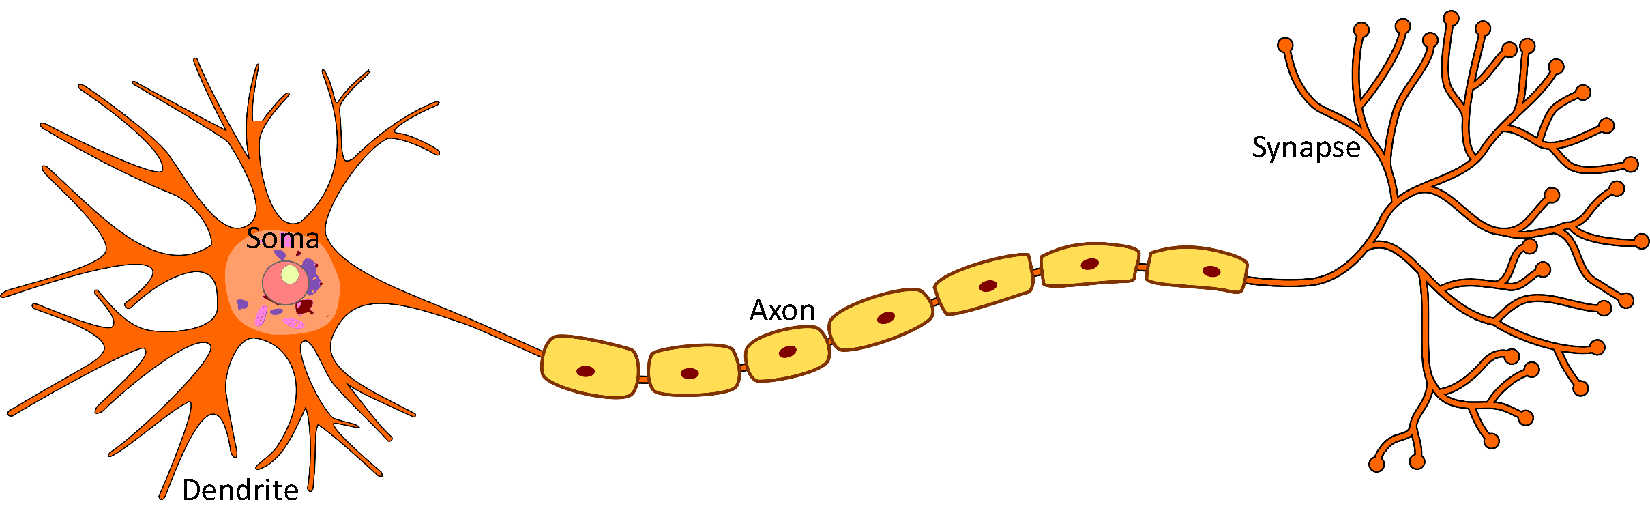
\includegraphics[width=\textwidth]{images/background/Neuron.pdf}
	\caption[Illustration of a biological neuron]{Illustration of a biological neuron. Image modified from \cite{Neuron}.}
	\label{fig:neuron}
\end{figure}
\begin{figure}[htb!]
	\centering
	\begin{subfigure}[b]{0.8\textwidth}
		\centering
		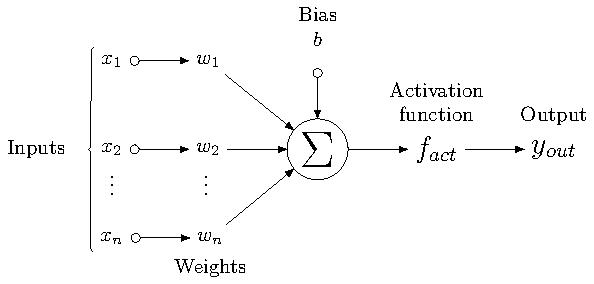
\includegraphics[width=\textwidth,keepaspectratio]{images/background/perceptron_perfect.pdf}
		\caption{Perceptron.}
		\label{fig:perceptron}
	\end{subfigure}
	\hfill
	\begin{subfigure}[b]{\textwidth}
		\centering
		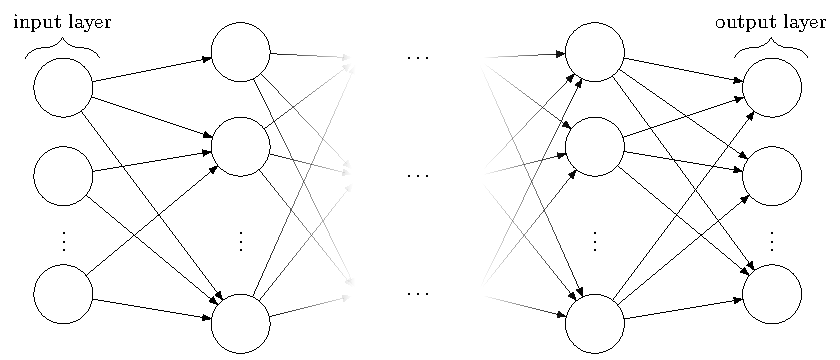
\includegraphics[width=\textwidth,keepaspectratio]{images/background/MLP.pdf}
		\caption{Multilayer perceptron (MLP).}
		\label{fig:MLP}
	\end{subfigure}
	
	\caption[Schematic representation of perceptron and multilayer perceptron]{Schematic representation of perceptron and multilayer perceptron (MLP). Images modified from \cite{Perceptrontex, MLPtex}.}
	\label{fig:percetron-mlp}
\end{figure}

The idea of convolution, a mathematical technique that entails swiping a tiny kernel over an image and computing the dot product between the kernel and the corresponding pixels in the image, serves as the foundation for CNNs. By spotting patterns in the data, this procedure aids in the extraction of features from the image. A feature map, which highlights particular aspects of the image such as edges, corners, and textures, is the result of this operation. The convolution operation is shown in Equation \ref{eq:conv1} \cite{Goodfellow-et-al-2016}.
\begin{equation}\label{eq:conv1}
	S(i, j)=(I * K)(i, j)=\sum_m \sum_n I(m, n) K(i-m, j-n)
\end{equation}
where $S$ is the output feature map, $I$ is the input image, $K$ is the kernel of size $m \times n$, $*$ represents the convolution operation, $i$ and $j$ are the row and column indexes of an element from $S$. The convolution is commutative, so the equation can be also written as:
\begin{equation}\label{eq:conv1}
	S(i, j)=(I * K)(i, j)=\sum_m \sum_n I(i-m, j-n) K(m,n)
\end{equation} 
Many deep learning libraries uses cross-correlation function in place of convolution as shown in Equation \ref{eq:cross-core}.
\begin{equation}\label{eq:cross-core}
	S(i, j)=(I * K)(i, j)=\sum_m \sum_n I(i+m, j+n) K(m,n)
\end{equation}
Cross-correlation is not commutative but has similar properties as convolution. A convolution operation on a two dimensional input image is illustrated in Figure \ref{fig:conv2dillustration}. Stride and padding are frequently used with convolution operation. Stride specifies how many pixels the kernel moves after each convolution operation i.e. the sliding of the kernel between the production of each output element. Padding is the process of adding empty pixels around the border of an input image. Padding is used to maintain image size and also for finding patterns in borders with full convolution on edge pixels.
To decrease the dimensionality of the feature maps and boost computing efficiency, CNNs use pooling layers in addition to convolutional layers. Downsampling is normally carried out by pooling layers using the maximum or average value of a set of adjacent pixels in the feature map as illustrated in Figure \ref{fig:poolingillustration}. Pooling also helps for making the model invariant to subtle translational changes in input. Convolutional, pooling, and fully connected layers are some of the layers of interconnected nodes that make up a CNN. The final classification or regression operation is carried out by the fully connected layers. Figure \ref{fig:CNN-schematic} shows a schematic representation of a CNN which stacks convolutional layers with an activation function applied after the convolution operation, pooling layers, and fully connected layers with activation functions.  Although, vision transformers \cite{Henry2022} are gaining a lot of popularity for various vision related tasks including medical imaging, modern CNN architectures like ConvNext \cite{liu2022convnet} and EfficientNetV2 \cite{EfficinetNetV2Ref} compete on par with them. Section \ref{sec:CNN-archis} contains brief descriptions of the CNN architectures used in this thesis.

\begin{figure}[htb!]
	\centering
	\begin{subfigure}[b]{0.8\textwidth}
		\centering
		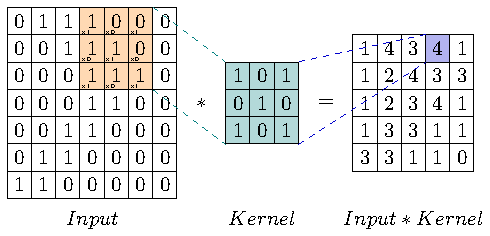
\includegraphics[width=\textwidth,keepaspectratio]{images/background/conv2d.pdf}
		\caption{Illustration of a convolution operation \cite{Conv2D}.}
		\label{fig:conv2dillustration}
	\end{subfigure}
	\hfill
	\begin{subfigure}[b]{0.7\textwidth}
		\centering
		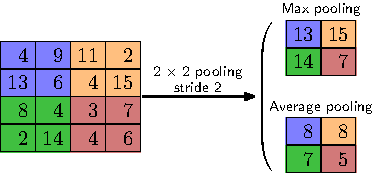
\includegraphics[width=\textwidth,keepaspectratio]{images/background/Pooling.pdf}
		\caption{Illustration of pooling operation.}
		\label{fig:poolingillustration}
	\end{subfigure}
	\hfill
	\begin{subfigure}[b]{\textwidth}
		\centering
		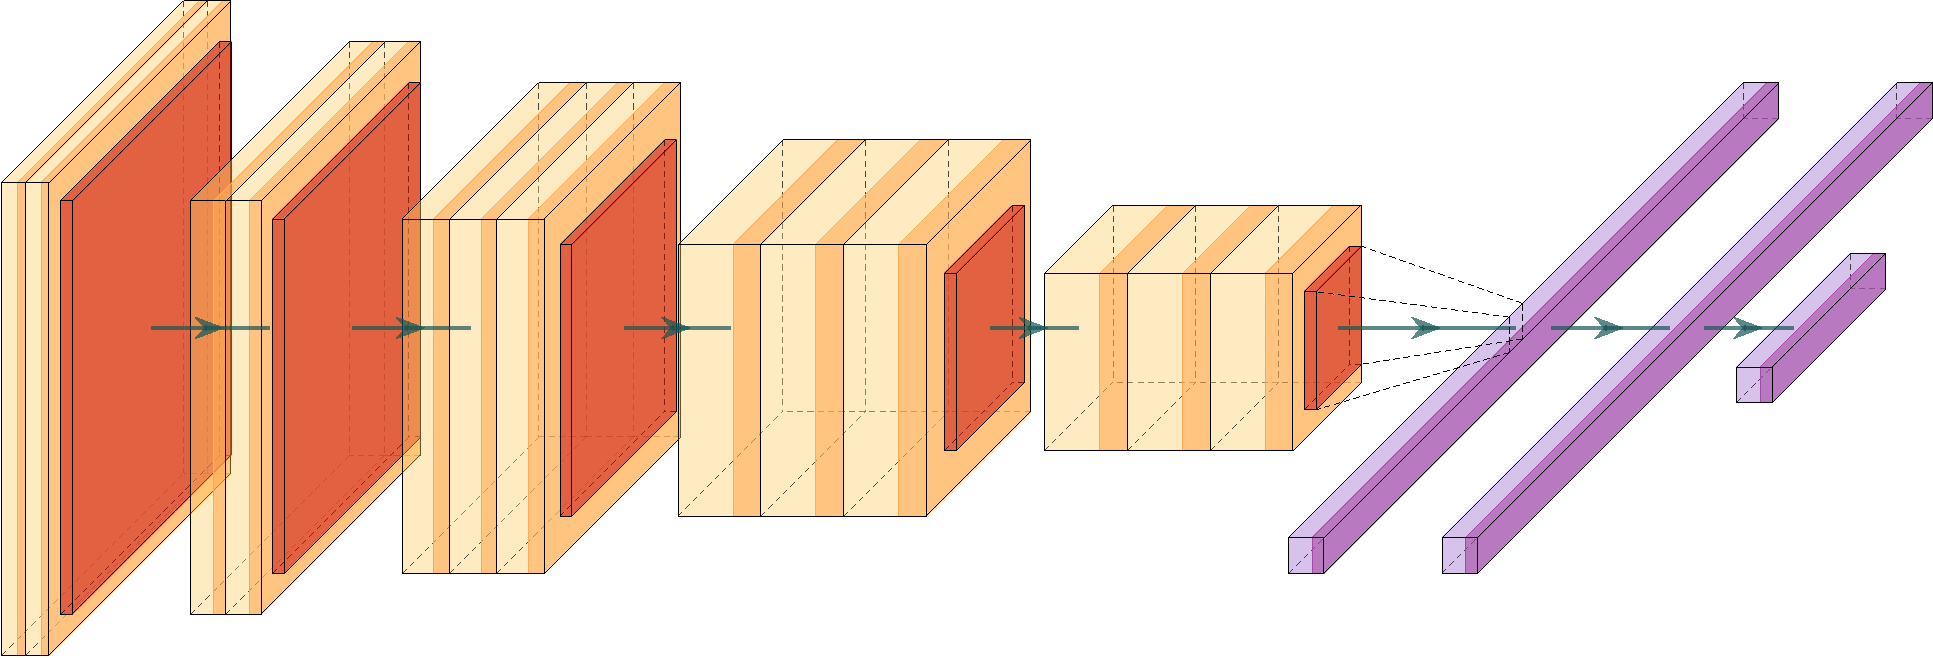
\includegraphics[width=\textwidth,keepaspectratio]{images/background/CNN-schematic.pdf}
		\caption{Schematic representation of a convolutional neural network. The yellow, and violet boxes with shaded endings represent convolutional and fully connected layers respectively with activation function. The red box represents pooling layer.}
		\label{fig:CNN-schematic}
	\end{subfigure}
	
	\caption{Schematic representation of convolution operation, pooling operation and convolutional neural network.}
	\label{fig:conv-CNN-schematic}
\end{figure}
%%%%%%%%%%%%%%%%%%%%%%%%%%%%%%%%%%%%%%%%%%%%%%%%%%%%%%%%%%%%%%%%%%%%%%%%
\subsection{Decision Tree}\label{sec:DecTree}
%%%%%%%%%%%%%%%%%%%%%%%%%%%%%%%%%%%%%%%%%%%%%%%%%%%%%%%%%%%%%%%%%%%%%%%%
Decision tree is a supervised learning algorithm, which can be utilized for both regression and classification tasks \cite{quinlan1986induction,BreiFrieStonOlsh84}. In this thesis, we are focusing on the decision tree for classification task. Decision tree represents a classifier as a recursive partition of instance space using a set of splitting rules \cite{quinlan1986induction,BreiFrieStonOlsh84}. These rules are easy to visualize and interpret with tree diagrams. Decision tree is a directed tree with no incoming edges at the root node and each of the other nodes has just one incoming edge. A decision or leaf or terminal node is a node without outgoing edges. All other nodes are called test or internal nodes. The instance space is divided into two or more sub-spaces by each test node based on a discrete function of input attribute values. Each decision node is given a class that corresponds to the best suitable target value. Instances are classified according to the test results by navigating from the tree's root to a leaf.

Figure \ref{fig:ex-dtree-dataset} shows an example training dataset and Figure \ref{fig:ex-dtree} shows the corresponding decision tree for deciding about playing golf (Yes/No) based on predictors like Outlook (Sunny/Overcast/Rainy), Temperature (Hot/Cool/Mild), Humidity (High/Normal), and Wind (Weak/Strong) \cite{DecTreeExample}. The red, yellow, and green boxes represent root, internal, and decision nodes respectively.
\begin{figure}[htb!]
	\centering
	\begin{subfigure}[b]{0.6\textwidth}
		\centering
		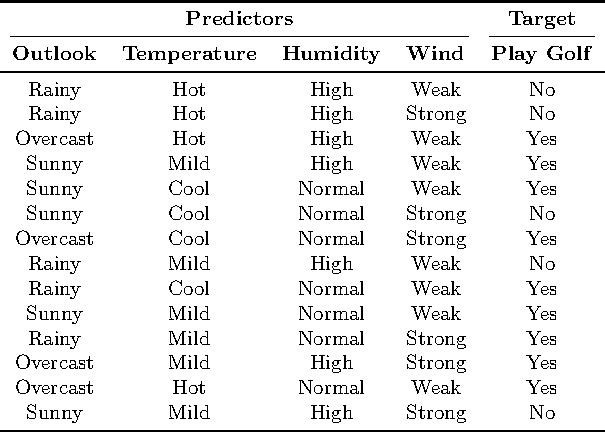
\includegraphics[width=\textwidth,keepaspectratio]{images/background/Decision_Tree_Table.pdf}
		\caption{Training dataset.}
		\label{fig:ex-dtree-dataset}
	\end{subfigure}
	\hfill
	\begin{subfigure}[b]{\textwidth}
		\centering
		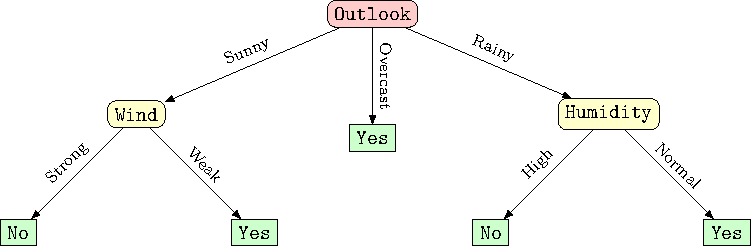
\includegraphics[width=\textwidth,keepaspectratio]{images/background/decision_tree_new.pdf}
		\caption{Decision tree.}
		\label{fig:ex-dtree}
	\end{subfigure}
	
	\caption[An example of decision tree]{An example of a decision tree for deciding about playing golf (Yes/No) based on predictors like Outlook (Sunny/Overcast/Rainy), Temperature (Hot/Cool/Mild), Humidity (High/Normal), and Wind (Weak/Strong) \cite{DecTreeExample}.  The red, yellow, and green boxes represent root, internal, and decision nodes respectively.}
	\label{fig:DecTreeExample}
\end{figure}

%%%%%%%%%%%%%%%%%%%%%%%%%%%%%%%%%%%%%%%%%%%%%%%%%%%%%%%%%%%%%%%%%%%%%%%%
\subsection{Formal Concept Analysis and Concept Lattice}\label{sec:FCA}
%%%%%%%%%%%%%%%%%%%%%%%%%%%%%%%%%%%%%%%%%%%%%%%%%%%%%%%%%%%%%%%%%%%%%%%%
Formal concept analysis (FCA) is a method of generating a formal concept hierarchy from a set of objects and their properties \cite{Wille10.1007/978-94-009-7798-3_15}. FCA has found many applications in machine learning and bioinformatics \cite{Motameny10.1007/978-3-540-78137-0_17,EngelbertF10.1007/BFb0026700,nguifo1993prediction}. In FCA each concept represents objects that share a particular set of attributes. FCA computes concept lattice, a directed, acyclic graph by hierarchically ordering all formal concepts derived from tabular input data.

The notion of formal context is central to FCA. Formal context is a triple \(\left\langle O,Y, I\right\rangle\) where \( O\) is a set of objects, \( Y\) is a set of attributes, and incidence \( I\subseteq O\times Y\) is a binary relation. A pair \(\left\langle A,B\right\rangle\)  is a formal concept of \(\left\langle O,Y, I\right\rangle\) provided that \( A\subseteq O\), \( B\subseteq Y\), \( A^{\uparrow } = B\), and \( B^{\downarrow } = A\) where,
%\begin{align}
%	A^{\uparrow } = \{ y\in Y\vert for\;each\;o\in A:\left\langle o,y\right\rangle \in I\}\ \\
%	B^{\downarrow } = \{ o\in O\vert for\; each\; y\in B:\left\langle o,y\right\rangle \in I\}
%\end{align}
\begin{gather}
	A^{\uparrow } = \{ y\in Y\vert for\;each\;o\in A:\left\langle o,y\right\rangle \in I\}\ \\
	B^{\downarrow } = \{ o\in O\vert for\; each\; y\in B:\left\langle o,y\right\rangle \in I\}
\end{gather}
$A$ is called the extent and $B$ is called the intent of a concept \(\left\langle A,B\right\rangle\). Formal concepts are ordered naturally by subconcept-superconcept relation defined as follows:
\begin{equation}\label{eq:FCARelation}
	\left\langle A_{1},B_{1}\right\rangle \leq\left\langle A_{2},B_{2}\right\rangle  \Longleftrightarrow  A_{1}\subseteq A_{2}(\Longleftrightarrow B_{2}\subseteq B_{1})
\end{equation}
For a formal context \(\left\langle O,Y, I\right\rangle\) the set \(\mathfrak{B}(O,Y,I)\) of all formal concepts with the ordering shown in Equation (\ref{eq:FCARelation}) is called the concept lattice.

Figure \ref{fig:example-FC} shows a sample formal context in a tabular form called a cross-table. The table rows represent objects and the columns represent attributes. An entry $\times$ in the table represents that the corresponding object has the corresponding attribute. Figure \ref{fig:example-CL} shows the concept lattice built from the formal context. Each node represents a formal concept by listing objects that share a set of attributes. The number within a circle beside the node is added to identify a node and for explanation purposes only. Within each node, the bottom box lists the objects i.e. the extent and the top box lists the attributes shared by the objects i.e. the intent of the concept. For example, the intent and extent of node \circled{2}  are $\left\{ c,d \right\}$ and $\left\{ 2,3,4,5 \right\}$ respectively. The lines in the lattice represent subconcept-superconcept relationship. For example, the formal concept represented by node \circled{4} is a subconcept of the formal concept represented by node \circled{2} because the extent of node \circled{4} is a subset of the extent of node \circled{2}  and the intent of node \circled{4} is a superset of the intent of node \circled{2}. 
\begin{figure}[htb!]
	\centering
	\begin{subfigure}[b]{0.39\textwidth}
		\centering
		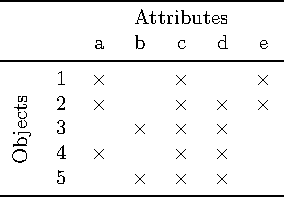
\includegraphics[width=\textwidth,keepaspectratio]{images/background/FCA-conext-ex.pdf}
		\caption{Formal context.}
		\label{fig:example-FC}
	\end{subfigure}
	\hfill
	\begin{subfigure}[b]{0.6\textwidth}
		\centering
		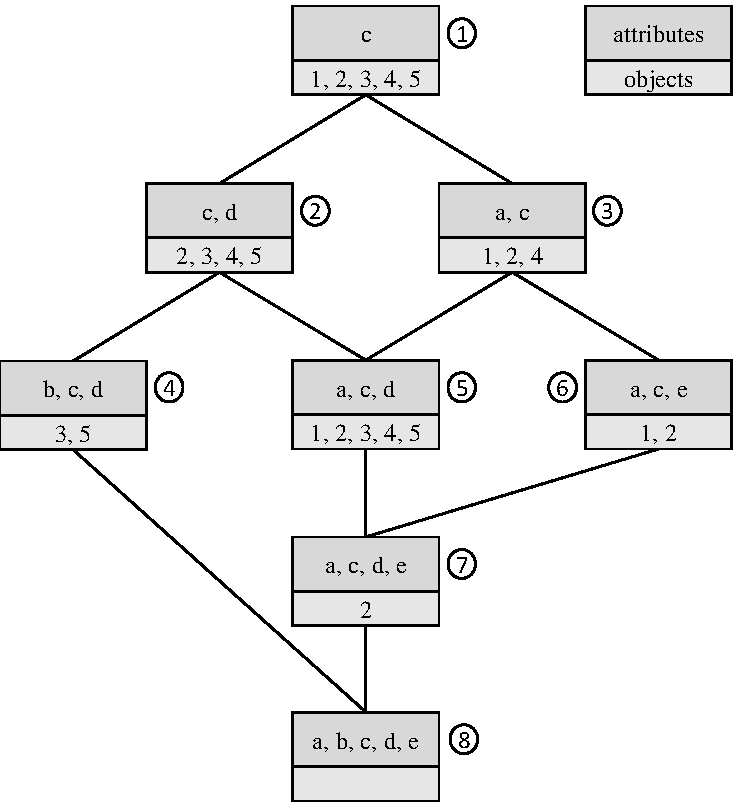
\includegraphics[width=\textwidth,keepaspectratio]{images/background/FCA-lattice-ex.pdf}
		\caption{Concept lattice.}
		\label{fig:example-CL}
	\end{subfigure}
	
	\caption[Example of a formal context in tabular form and corresponding concept lattice]{Example of a formal context in tabular form and corresponding concept lattice. An entry $\times$ in the context table represents that the corresponding object has the corresponding attribute.}
	\label{fig:example-FC-CL}
\end{figure}

%%%%%%%%%%%%%%%%%%%%%%%%%%%%%%%%%%%%%%%%%%%%%%%%%%%%%%%%%%%%%%%%%%%%%%%%
\subsection{Gaussian Mixture Model}\label{sec:GMM}
%%%%%%%%%%%%%%%%%%%%%%%%%%%%%%%%%%%%%%%%%%%%%%%%%%%%%%%%%%%%%%%%%%%%%%%%
A Gaussian mixture model (GMM) is a probability density function represented as the weighted sum of component Gaussian densities  \cite{Reynolds2009}. The mixture represents a normally distributed overall population whereas the components represent subpopulations within the whole population. For one-dimensional data, a GMM with $M$ components can be defined as:
\begin{equation}
	\hat{f}_{GMM}\left(x\right) =  \sum_{m = 1}^{M}\varnothing_{m}\mathcal{N}\left(x\right\vert  \mu_{m},\sigma_{m})
\end{equation}
where, \(\varnothing_{m} \geq 0\) is the mixture weight i.e. the probability of \( m\)-th component \( \kappa_{m}\) satisfying \( \sum_{m = 1}^{M}\varnothing_{m} = 1\)  so that the total probability distribution normalizes to $1$, and \(\mathcal{N}\left(x\right\vert  \mu_{m},\sigma_{m})\) is the distribution of a Gaussian component with mean \( \mu_{m}\) and standard deviation \( \sigma_{m}\) defined as:
\begin{equation}
	\mathcal{N}\left(x\right\vert  \mu_{m},\sigma_{m}) =\frac{1}{\sigma_{m}\sqrt{2\pi }}e^{-\frac{1}{2}\left(\frac{x-\mu_{m}}{\sigma_{m}}\right)^{2}}
\end{equation}

Expectation-Maximization, an iterative unsupervised learning technique can be used to determine the parameters of GMM \cite{Dempster1977}. Steps involved in Expectation-Maximization for \( n\)  data points \( X = \{ x_{t}\vert t = 1,\ldots ,n\}\)  are:
\begin{itemize}
	\item Guess initial values for GMM parameters denoted by \(\hat{\mu }_{m},\hat{\sigma }_{m},\)  and \( \hat{\varnothing }_{m}\)  respectively.
	
	\item  Expectation step: calculate \(\hat{\gamma }_{t,m}\) , the probability of a point \( x_{t}\)  being generated by \( \kappa_{m}\)
	
	\begin{equation}
		\hat{\gamma }_{t,m} = \frac{\hat{\varnothing }_{m}\mathcal{N}\left(x_{t}\right\vert \hat{\mu }_{m},\hat{\sigma }_{m})}{\sum_{r = 1}^{M}\hat{\varnothing }_{r}\mathcal{N}\left(x_{t}\right\vert \hat{\mu }_{r},\hat{\sigma }_{r})}
	\end{equation}
	
	\item Maximization step: Update GMM parameters using the following equations:
	\begin{equation}
		\hat{\mu }_{m} =\frac{\sum_{t = 1}^{n}\hat{\gamma }_{t,m}x_{t}}{\sum_{t = 1}^{n}\hat{\gamma }_{t,m}}
	\end{equation}
	
	\begin{equation}
		\hat{\sigma }_{m} =\sqrt{\frac{\sum_{t = 1}^{n}\hat{\gamma }_{t,m}(x_{t}-\hat{\mu }_{m})^{2}}{\sum_{t = 1}^{n}\hat{\gamma }_{t,m}}}
	\end{equation}
	
	\begin{equation}
		\hat{\varnothing }_{m} = \sum_{t = 1}^{n}\frac{\hat{\gamma }_{t,m}}{n}
	\end{equation}
	
	\item Repeat Expectation and Maximization steps until the total likelihood $L$ converges, where
	\begin{equation}
		L = \prod_{t = 1}^{n}\hat{f}_{GMM}\left(x_{t}\right)
	\end{equation}
\end{itemize}

Information criterion tests like Akaike Information Criteria (AIC) \cite{Akaike1974} and Bayesian Information Criteria (BIC) \cite{Schwarz2007} can be used to select an appropriate GMM by penalizing the number of free parameters to prevent overfitting. AIC and BIC can be defined as:
\begin{equation}
	AIC = 2p+2\ln L
\end{equation}
\begin{equation}
	BIC = p\ln L+2\ln L
\end{equation}
where $p$ is the number of free parameters and $\ln$ is the natural logarithm. The preferred GMM is the one with minimum AIC and BIC values.

%%%%%%%%%%%%%%%%%%%%%%%%%%%%%%%%%%%%%%%%%%%%%%%%%%%%%%%%%%%%%%%%%%%%%%%%
\subsection{Kernel Density Estimation}\label{sec:KDE}
%%%%%%%%%%%%%%%%%%%%%%%%%%%%%%%%%%%%%%%%%%%%%%%%%%%%%%%%%%%%%%%%%%%%%%%%
Kernel density estimation (KDE) is a non-parametric way of estimating the probability density function of an independent and identically distributed random variable \cite{Parzen1962,Rosenblatt1956}. For \( n\)  data points \( X = \{ x_{t}\vert t = 1,\ldots ,n\}\), KDE is calculated as:
\begin{equation}
	\hat{f}_{KDE}\left(x\right) = \frac{1}{nh}\sum_{t = 1}^{n}K\left(\frac{x-x_{t}}{h}\right)
\end{equation}
where \( h\) is the bandwidth and \( K\) is the kernel function. If a Gaussian kernel function is used to estimate the density of univariate data then the bandwidth can be selected using Silverman’s rule of thumb \cite{Silverman2018} as shown in the following equation:
\begin{equation}
	h=0.9 min\left (\hat{\sigma},\frac{IQR}{1.34}\right)n^{\frac{-1}{5}}
\end{equation}
where \( IQR\) is the interquartile range and \(\hat{\sigma }\) is the standard deviation of the samples.


%%%%%%%%%%%%%%%%%%%%%%%%%%%%%%%%%%%%%%%%%%%%%%%%%%%%%%%%%%%%%%%%%%%%%%%%
\subsection{Transfer Learning and Pre-training strategies}\label{sec:TL}
%%%%%%%%%%%%%%%%%%%%%%%%%%%%%%%%%%%%%%%%%%%%%%%%%%%%%%%%%%%%%%%%%%%%%%%%
Transfer learning is a collection of techniques to enhance the performance of a model on a target task using the information that a model acquires during training on a source task, even if the two tasks are dissimilar \cite{5288526}. Transfer learning focuses on knowledge adaptation and it is defined using two concepts: domains and tasks. A domain $\mathcal{D}=\left \{ \mathcal{X},P(X) \right \}$ has two components: A feature space $\mathcal{X}$ and a marginal probability distribution $P(X)$ where $X=\left \{ x_{1},\cdots ,x_{n} \right \} \in \mathcal{X}$. For a domain $\mathcal{D}$ a task $\mathcal{T}=\left \{ \mathcal{Y},f(x) \right \}$ has two parts: A label space $\mathcal{Y}$ and a predictive function $f:\mathcal{X}\rightarrow\mathcal{Y}$, that can be learned from training data of pairs $\left \{ x_{i},y_{i} \right \}$ where $ x_{i} \in X, y_{i} \in \mathcal{Y}$. Pan and Yang \cite{5288526} defined transfer learning as:
\begin{definition}[Transfer Learning]
	\enquote{Given a source domain $\mathcal{D}_S$ and learning task $\mathcal{T}_S$, a target domain $\mathcal{D}_T$ and learning task  $\mathcal{T}_T$, transfer learning aims to help improve the learning of the target predictive function $f_T(\cdot)$ in  $\mathcal{D}_T$ using the knowledge in  $\mathcal{D}_S$ and  $\mathcal{T}_S$, where $\mathcal{D}_S \neq \mathcal{D}_T$, or $\mathcal{T}_S \neq \mathcal{T}_T$} \cite{5288526}.
\end{definition}

\noindent Plested and Gedeon \cite{Plested2022} defined deep transfer learning in the context of image classification as:
\begin{definition}[Deep Transfer Learning]
	\enquote{Given a source domain $\mathcal{D}_S$ and learning task $\mathcal{T}_S$, a target domain $\mathcal{D}_T$ and learning task  $\mathcal{T}_T$, transfer learning aims to help improve the performance of the target model $M$ on the target task $\mathcal{T}_T$ by initializing it with weights $W$ that are trained on source task  $\mathcal{T}_S$ using source dataset $D_{S}$ (pretraining), where $\mathcal{D}_S \neq \mathcal{D}_T$, or $\mathcal{T}_S \neq \mathcal{T}_T$} \cite{Plested2022}.
\end{definition}

Transfer learning can be broadly categorized into three settings based on $\mathcal{T}_S$, $\mathcal{T}_T$ and provided labels as shown in Figure \ref{fig:transfer-learn-taxonomy} \cite{Mao2020, Ruder2019Neural}. If $\mathcal{T}_S = \mathcal{T}_T$ with only source domain labels provided, it is called transductive transfer learning. When  $\mathcal{T}_S \neq \mathcal{T}_T$ with labels available for the target domain, it is called inductive transfer learning. If no labels are provided then it is called unsupervised transfer learning. Inductive transfer learning can be subdivided into multi-task and sequential transfer learning. $\mathcal{T}_S$ and $\mathcal{T}_T$ are simultaneously learned in multi-task learning whereas, in sequential transfer learning  $\mathcal{T}_S$ is first learned (pre-training stage), and then $\mathcal{T}_T$ is learned (fine-tuning stage). In this thesis, we are focusing on sequential transfer learning.
\begin{figure}[htb!]
	\centering
	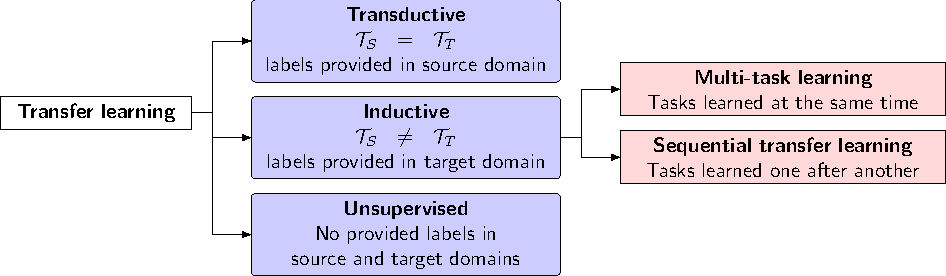
\includegraphics[width=\textwidth,,keepaspectratio]{images/background/transfer-learning-taxonomy.pdf}
	\caption[Transfer learning scenarios]{Transfer learning scenarios \cite{Mao2020, Ruder2019Neural}. $\mathcal{T}_S$ and $\mathcal{T}_T$ represent source and target tasks respectively.}
	\label{fig:transfer-learn-taxonomy}
\end{figure}

Pre-training in the context of transfer learning can be supervised or self-supervised (described in next para) \cite{Mao2020}. Supervised transfer learning uses a pre-trained model that was trained on a sizable dataset for a particular task as a starting point for a new task. A smaller dataset is used to fine-tune the pre-trained model on the new task in order to adapt it to the new task. For instance, a model that has already been trained on a huge image classification dataset like ImageNet \cite{Russakovsky2015} can be fine-tuned for a particular image classification job, like detecting cats vs dogs, on a smaller dataset. This strategy can save resources and shorten the training period and also increase the new model's accuracy.

Self-supervised pre-training uses a model that has already been trained on a related task that does not require labeled data as a starting point for a new task.  In self-supervised pre-training for image classification, the model is first taught to extract important features from images using unsupervised techniques like pretext tasks, generative modeling, or contrastive learning \cite{9462394}. A pretext task can be predicting a specific feature of the data, like predicting an image's rotation or hue. Generative modeling involves training the model to create realistic synthetic data.  Contrastive learning involves training the model to differentiate between negative and positive image pairs. Using this unsupervised pre-training technique the model learns a useful representation of the data which can be refined for a new downstream task on a  labeled dataset. When labeled data is hard to come by or expensive, this strategy can be especially helpful. We can use a source task with a lot of unlabeled examples and transfer the learned knowledge to an interesting target task thanks to the complementing research fields of self-supervised learning and transfer learning \cite{Mao2020}.

%%%%%%%%%%%%%%%%%%%%%%%%%%%%%%%%%%%%%%%%%%%%%%%%%%%%%%%%%%%%%%%%%%%%%%%%
\subsection{Visual Explanation of CNN Model}\label{sec:Grad-CAM}
%%%%%%%%%%%%%%%%%%%%%%%%%%%%%%%%%%%%%%%%%%%%%%%%%%%%%%%%%%%%%%%%%%%%%%%%
Explainability is important for AI tools especially in the case of medical applications \cite{Vellido2020} to understand how a model is taking its decision. Explainability techniques can be model-based (the model itself is explainable i.e. easy to be understood) vs post hoc (explains a trained model), model-specific (limited to particular types of models) vs model-agnostic (independent of the type of the model), and global (provides general relationships learned by the model in a dataset level) vs local (provides explanations for individual input) \cite{VanderVelden2022}. Visual explanation that shows regions of the input image that are significant for predictions from the model is common used for medical image analysis \cite{VanderVelden2022}. Grad-CAM \cite{Selvaraju2020} is a post hoc, model-specific technique for local visual explanation of CNNs. Grad-CAM uses gradient flowing into the ultimate convolution layer for producing heatmaps, and it is a kind of post-hoc attention that can be applied on an already trained model. Grad-CAM provides similar result to occlusion sensitivity map \cite{10.1007/978-3-319-10590-1_53} that works by masking patches of the input image, but Grad-CAM is much faster to calculate compared to image occlusion \cite{Selvaraju2020}.  Grad-CAM has been used for visual explanation in numerous medical image analysis tasks including brain \cite{10.3389/fnins.2020.00630}, breast \cite{ElAdoui2020}, cardiovascular \cite{Candemir2020}, chest \cite{Brunese2020}, dental \cite{8977504}, eye \cite{Martins2020}, female reproductive system \cite{9098587}, gastrointestinal \cite{Itoh2020}, lymph nodes \cite{Ji2019}, musculosketal \cite{VonSchacky2020}, thyroid \cite{Lee2020}, and skin \cite{Zunair2020} images. We utilized Grad-CAM technique for visualizing the regions of the input image that are significant for skin lesion class prediction from the CNN models (as shown in Figure \ref{fig:gradcam-example}) used in our study. 
\begin{figure}[htb!]
	\centering
	\begin{subfigure}[b]{0.4\textwidth}
		\centering
		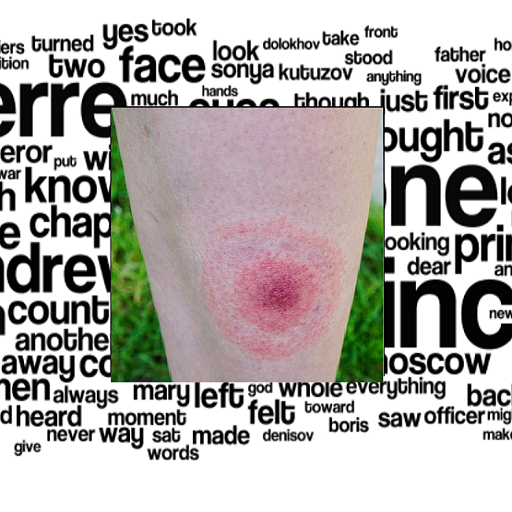
\includegraphics[width=\textwidth,keepaspectratio]{images/pretraining/gradcam/CenteredLyme9.png}
		\caption{Input image.}
		\label{fig:grad-input}
	\end{subfigure}
	\hfill
	\begin{subfigure}[b]{0.4\textwidth}
		\centering
		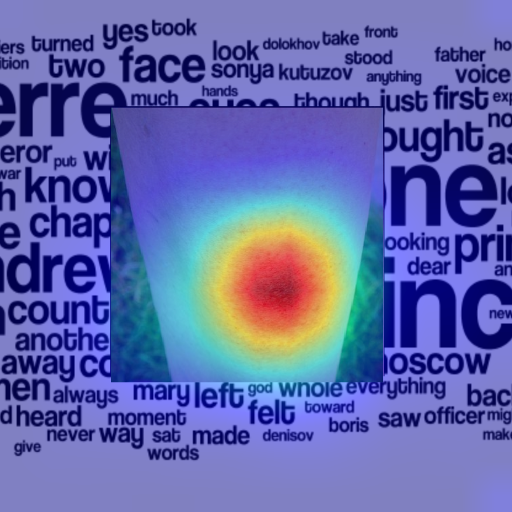
\includegraphics[width=\textwidth,keepaspectratio]{images/pretraining/gradcam/9/EfficientNetB5CombinedGradCam.png}
		\caption{Gard-CAM visualization.}
		\label{fig:grad-result}
	\end{subfigure}
	
	\caption{Gard-CAM visualization example.}
	\label{fig:gradcam-example}
\end{figure}

%%%%%%%%%%%%%%%%%%%%%%%%%%%%%%%%%%%%%%%%%%%%%%%%%%%%%%%%%%%%%%%%%%%%%%%%
\section{Literature Review}\label{sec:litreview}
%%%%%%%%%%%%%%%%%%%%%%%%%%%%%%%%%%%%%%%%%%%%%%%%%%%%%%%%%%%%%%%%%%%%%%%%
The following subsections review the related works on AI for skin lesion diagnosis, a brief overview of Lyme disease with the use of AI for Lyme disease diagnosis, and also the works on the data scarcity problem.
%%%%%%%%%%%%%%%%%%%%%%%%%%%%%%%%%%%%%%%%%%%%%%%%%%%%%%%%%%%%%%%%%%%%%%%%
\subsection{AI for Skin Disorder Diagnosis}
%%%%%%%%%%%%%%%%%%%%%%%%%%%%%%%%%%%%%%%%%%%%%%%%%%%%%%%%%%%%%%%%%%%%%%%%
Many works have been done utilizing deep learning techniques specifically convolutional neural networks (CNNs) for diagnosing cancerous and other common skin lesions from dermoscopic images. Haenssle et al. \cite{Haenssle2018} used transfer learning from ImageNet \cite{Russakovsky2015} pre-trained InceptionV4 CNN architecture for detecting melanoma skin cancer using images from International Skin Imaging Collaboration (ISIC) \cite{Codella2019} dermoscopic image archive and compared the model's performance against 58 dermatologists. CNN outperformed most of the expert dermatologists. Brinker et al. \cite{Brinker2019} also used ImageNet transfer learning with ResNet50 CNN architecture on a dataset of 12,378 dermoscopic images from ISIC archive for the melanoma classification task and compared the CNN's performance against dermatologists. Again deep learning outperformed 136 out of 157 dermatologists. Maron et al. \cite{Maron2019}] also used ResNet50 architecture with ImageNet transfer learning and performed a multiclass cancer classification using 11,444 dermoscopic images from ISIC archive where most of the images were taken from HAM10000 dataset \cite{Tschandl2018}. This study also showed the superiority of deep learning models compared to 112 dermatologists. 

Liu et al. \cite{Liu2020} trained an InceptionV4 based deep learning system using clinical skin lesion images and patient data from 16,114 verified cases for the differential diagnosis of 26 common skin conditions. Esteva et al. \cite{Esteva2017} trained an InceptionV3 CNN architecture on a dataset of 126,076 clinical skin lesion images and 3,374 dermoscopic images using ImageNet transfer learning for skin cancer classification. The deep learning model performed on par compared with 21 board-certified expert dermatologists. Han et al. \cite{Han2018} trained an ensemble model of ResNet152 and VGG19 CNN architectures using a dataset of 49,567 clinical skin lesion images of onychomycosis that outperformed most of the expert dermatologists.

Results from aforementioned studies confirmed that deep learning-based systems compete on par with expert dermatologists for diagnosing diseases from dermoscopic and clinical skin lesion images. Recent studies showed that incorporating data from multiple modalities in the analysis process significantly improves the artificial intelligence based models' performance compared to a single modality based analysis for many medical diagnosis tasks \cite{Senaratne10.1145/3556980, Li10.1145/3344256, Pacheco9364366, Chen2022}. Pacheco et al. \cite{Pacheco9364366} proposed an attention based deep learning approach for combining images and patient data for skin cancer classification that resulted in better performance compared to a single modality based analysis. Chen et al. \cite{Chen2022} showed a 9 percent improvement in model accuracy with a multimodal fusion of skin image and clinical data compared to image only skin cancer classification. 

%%%%%%%%%%%%%%%%%%%%%%%%%%%%%%%%%%%%%%%%%%%%%%%%%%%%%%%%%%%%%%%%%%%%%%%%
\subsection{AI for Lyme Disease Diagnosis}
%%%%%%%%%%%%%%%%%%%%%%%%%%%%%%%%%%%%%%%%%%%%%%%%%%%%%%%%%%%%%%%%%%%%%%%%
Lyme disease is an infectious disease transmitted by ticks and caused by pathogenic bacteria of the \textit{Borrelia burgdorferi} sensu lato group \cite{Shapiro2014}. It is estimated that around 476,000 people in the United States and more than 200,000 people in western Europe are affected by Lyme disease each year \cite{Marques2021}. Most of the time an expanding round or oval red skin lesion known as erythema migrans (EM) becomes visible in the victim’s body which is the most common early symptom of Lyme disease \cite{Shapiro2014, Burlina2018}. EM usually appears at the site of a tick bite after one to two weeks (range, 3 to 30 days) as a small redness and expands almost a centimeter per day, creating the characteristic bull’s-eye pattern as shown in Figure \ref{fig:EM-bullseye} \cite{Shapiro2014, Burlina2018, Strle2009, Berglund1995}. EM generally vanishes within a few weeks or months but the Lyme disease infection advances to affect the nervous system, skin, joints, eyes, and heart \cite{Shapiro2014, Strle2009}. Antibiotics can be used as a medium of effective treatment in the early stage of Lyme disease. So, early recognition of EM is extremely important to avoid long-term complications of Lyme disease. 

Most European and North American guidelines recommend a two-tier serology test to detect antibodies against \textit{Borrelia burgdorferi} sensu lato for diagnosing Lyme disease \cite{Eldin2019, Trevisan2020}. However, a serology test is only recommended in the absence of EM because early serology has low sensitivity (40\% to 60\%) and may result in false negatives \cite{Eldin2019}. Alternatively, direct detection of Borrelia burgdorferi sensu lato can be done using culture, microscopy, or PCR \cite{Trevisan2020}. The gold standard of microbiological diagnosis - the culture of bacteria requires laboratory expertise and special media for \textit{Borrelia burgdorferi} sensu lato \cite{Eldin2019}. Light microscopy-based detection is not feasible in clinical practice \cite{Trevisan2020}. PCR based diagnosis is also very difficult and shows highly variable sensitivity \cite{Trevisan2020}. Direct detection methods are not always feasible for clinicians because of extended processing time and required expertise \cite{Burlina2020}. The diagnosis of EM is a challenging task because EM can create different patterns instead of the trademark bull’s-eye pattern as shown in Figure \ref{fig:EM-atypical}.

Despite the vast application of AI in the field of skin lesion diagnosis, there are only a few works related to Lyme disease detection from EM skin lesion images. The unavailability of reliable public EM datasets as a result of privacy concerns of medical data may be the reason for the lack of extensive studies in this field. The only publicly available dataset of EM is a small collection of web-scraped unverified images hosted in a kaggle repository \cite{LymeDatasetKaggle}. Čuk et al. \cite{Cuk2014} proposed a visual system for EM recognition on a private EM dataset using classical machine learning techniques including naïve Bayes, SVM, boosting, and neural nets (not deep learning). They considered ellipse, the common shape of EM, and used eccentricity, small and large axis ratio, ellipse angular, and ellipse focus attributes for classification. Deep learning techniques learn image features from training images via an optimization process and recent studies show that image features extracted by deep learning techniques outperform human-engineered image features for medical image classification tasks \cite{Burlina2020}. Burlina et al. \cite{Burlina2018} created a dataset of EM by collecting images from the internet and trained a CNN architecture ResNet50 as a binary classifier to distinguish between EM and other skin conditions. Although their dataset is not public, the trained model is publicly available. Burlina et al. \cite{Burlina2020} further enriched the dataset with more images from the East Coast and Upper Midwest of the United States and trained six CNNs namely ResNet50, InceptionV3, MobileNetV2, DenseNet121, InceptionResNetV2, and ResNet152 for EM classification. They did not make the dataset or the trained models public for the extended study. Burlina et al. \cite{Burlina2018} and Burlina et al. \cite{Burlina2020} used transfer learning from ImageNet pre-trained models and studied the CNNs in terms of predictive performance. Koduru et al. \cite{Koduru2021} deployed a trained ResNet50 CNN model utilizing a private dataset  for a prototype application to identify EM. Jacob et al. \cite{Jacob2022} used the kaggle Lyme dataset \cite{LymeDatasetKaggle} to test state-of-the-art self-supervised learning techniques against supervised transfer learning for different CNN architectures and comparatively self-supervised learning underperformed. Oholtsov et al. \cite{Oholtsov2023} suggested using both clean and dirty images for training EM classifier based on experimentation using an unverified dataset of only 106 EM images.

\begin{figure}[htb!]
	\centering
	\begin{subfigure}[b]{0.4\textwidth}
		\centering
		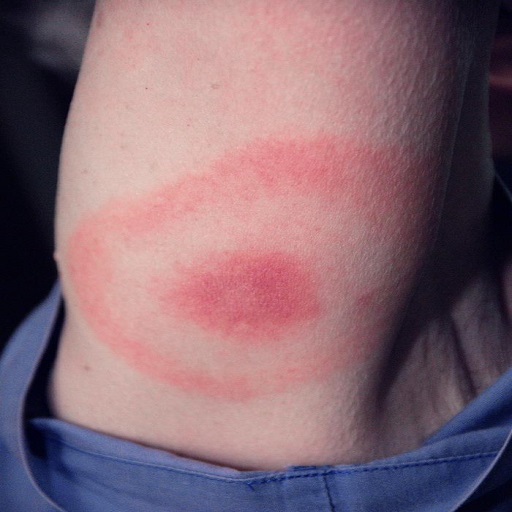
\includegraphics[width=\textwidth,keepaspectratio]{images/background/EM_bullseye.jpg}
		\caption{Bull’s-eye pattern.}
		\label{fig:EM-bullseye}
	\end{subfigure}
	\hfill
	\begin{subfigure}[b]{0.4\textwidth}
		\centering
		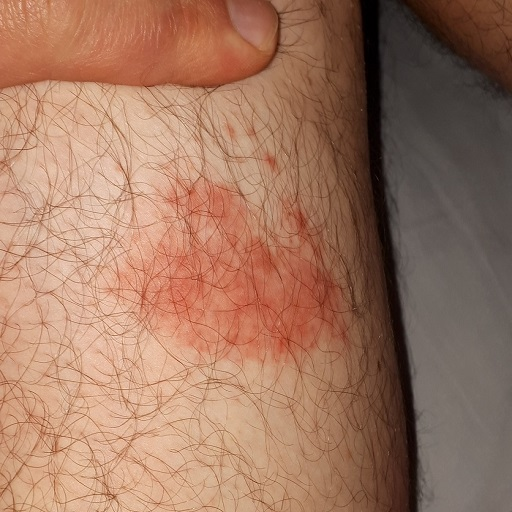
\includegraphics[width=\textwidth,keepaspectratio]{images/background/EM_atypical.jpg}
		\caption{Atypical pattern.}
		\label{fig:EM-atypical}
	\end{subfigure}
	
	\caption[Patterns of erythema migrans]{Patterns of erythema migrans (EM) \cite{EMPatterns}.}
	\label{fig:EM-patterns}
\end{figure}

%%%%%%%%%%%%%%%%%%%%%%%%%%%%%%%%%%%%%%%%%%%%%%%%%%%%%%%%%%%%%%%%%%%%%%%%
\subsection{Related Works on Data Scarcity}\label{RelWorkDataScarcity}
%%%%%%%%%%%%%%%%%%%%%%%%%%%%%%%%%%%%%%%%%%%%%%%%%%%%%%%%%%%%%%%%%%%%%%%%
Transfer learning and expanding data by transforming images with augmentation techniques are frequently used by researchers to improve deep learning model's performance on limited image datasets. Perez et al \cite{Perez2018} showed that using data augmentation significantly improves model's performance using InceptionV4, ResNet, and DenseNet architectures for melanoma classification with dermoscopic images from ISIC archive. P{\'{e}}rez et al. \cite{Perez2021} showed that combining transfer learning and data augmentation significantly improves model's performance for melanoma diagnosis from images using an extensive experimental study on 11 datasets and 12 CNN architectures. 

Transfer learning with supervised ImageNet\cite{Russakovsky2015} pre-training is frequently used in medical image analysis tasks \cite{10.1117/12.2531198, 7950523, McKinney2020, Liu2020, Graziani2019VisualizingAI, Heker2020}. Transfer learning from natural images of ImageNet provides performance improvement according to multiple empirical studies \cite{app10134523, Graziani2019VisualizingAI, Heker2020}. Even if this strategy does not guarantee an improvement in performance Raghu et al. \cite{Raghu2019} showed using a detailed study that it speeds up convergence and is especially helpful for training with limited data. Gu et al. \cite{GuRef} showed that progressive transfer learning starting from an ImageNet pre-trained model end-to-end fine-tuned on a dataset of similar skin lesions with a slight domain shift increases the classification performance of skin cancer classification task for a smaller dataset. Recently, self-supervised pre-training using unlabeled domain-specific data is gaining popularity in medical image analysis \cite{9710396, He2020.04.13.20063941, 9010639, 10.1007/978-3-030-59710-8_39, https://doi.org/10.48550/arxiv.2211.08559, https://doi.org/10.48550/arxiv.2010.05352}. Azizi et al. \cite{9710396} showed that training a model on ImageNet in self-supervised fashion followed by self-supervised learning on unlabeled in-domain medical images, and fine-tuning end-to-end for downstream supervised tasks significantly improves model accuracy. They used ResNet architectures on X-ray and dermatology classification tasks for experimentation. Dadsetan et al. \cite{https://doi.org/10.48550/arxiv.2211.08559} also showed that combining ImageNet and domain-specific self-supervised pre-training gives better performance for Alzheimer's disease propagation from brain magnetic resonance imaging.

For multimodal training i.e. training utilizing all the available modalities (for example, image modality and patient data modality), the general assumption is that both the training and test data will have full and paired modalities \cite{ngiam2011multimodal,Zadeh2017}. However, missing data is common for real-world clinical scenarios \cite{Huang2020}. Existing works in the literature generally drop the incomplete samples or impute missing values \cite{ma2021smil, 10.1145/3534678.3539388}. Some studies report improvements by dropping incomplete samples \cite{10.1145/3308558.3313643, wang2020multimodal}. Generative models are used in many studies for imputing missing modalities \cite{LI2020105592, 10.1145/3219819.3219963, pan2021disease}. Ma et al. \cite{ma2021smil} approximated missing modality using modality priors learned from dataset. Chen et al. \cite{10.1145/3394486.3403182} fused multimodal incomplete data using a heterogeneous graph structure. Zhang et al. \cite{10.1145/3534678.3539388} considered auxiliary data from similar neighbors of a patient to deal with missing modalities. If paired data is missing for the modalities but training data for individual modalities are available then individual classifiers can be trained for each modality and the results can be fused using a weighing scheme \cite{rahate2022multimodal}.

%%%%%%%%%%%%%%%%%%%%%%%%%%%%%%%%%%%%%%%%%%%%%%%%%%%%%%%%%%%%%%%%%%%%%%%%


\section{Research Questions and Challenges}\label{sec:research-questions}
%%%%%%%%%%%%%%%%%%%%%%%%%%%%%%%%%%%%%%%%%%%%%%%%%%%%%%%%%%%%%%%%%%%%%%%%
Pre-training with in-domain images is effective for increasing the performance of deep CNN based image classifiers however it is difficult to collect a large number of in-domain images for many skin conditions like EM. The dataset created as part of our study for EM analysis consists of clinical skin lesion images. First, we thought of pre-training a CNN for EM classification using clinical skin lesion images of other skin lesions as we could not collect a large number of in-domain unlabeled samples related to EM. Most of the accessible datasets are concerned with skin cancers. Wen et al. \cite{WEN2022e64} systematically reviewed the available datasets for skin cancers. Out of the open access clinical skin lesion image datasets, SD-198 \cite{sun2016benchmark} containing 6,584 clinical skin lesion images and its extended version SD-260 \cite{8736039} containing 20,600 clinical skin lesion images of skin cancer images seemed promising but these datasets are not easily accessible \footnote{ The download link mentioned in the paper did not work and we did not get any response from the authors after asking for access.}. On the contrary, dermoscopic image datasets like HAM10000 dataset \cite{Tschandl2018} are easily accessible. The image modality of clinical EM dataset is quite different from dermoscopic images of HAM10000 dataset as shown in Figure \ref{fig:EM-bullseye2} and \ref{fig:dermo-sample}. Our first research question is:
%\begin{tcolorbox}[width=\textwidth]   
\begin{researchquestion}\label{question1}
	Can we improve the performance of ImageNet pretrained clinical skin lesion image classifier's performance with additional pre-training using dermoscopic images?
\end{researchquestion}
%\end{tcolorbox} 

\begin{figure}[htb!]
	\centering
	\begin{subfigure}[b]{0.3\textwidth}
		\centering
		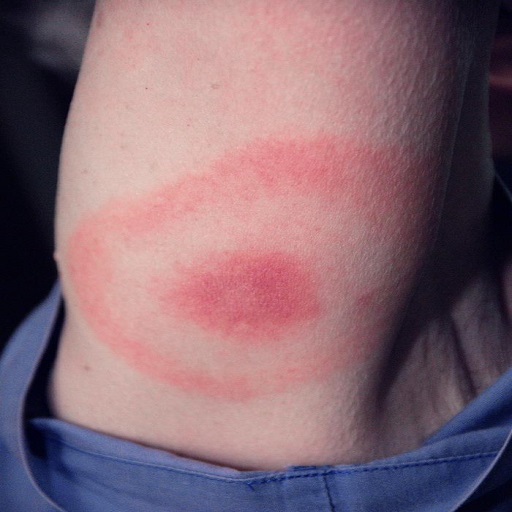
\includegraphics[width=\textwidth,keepaspectratio]{images/background/EM_bullseye.jpg}
		\caption{Clinical image.}
		\label{fig:EM-bullseye2}
	\end{subfigure}
	\hfill
	\begin{subfigure}[b]{0.3\textwidth}
		\centering
		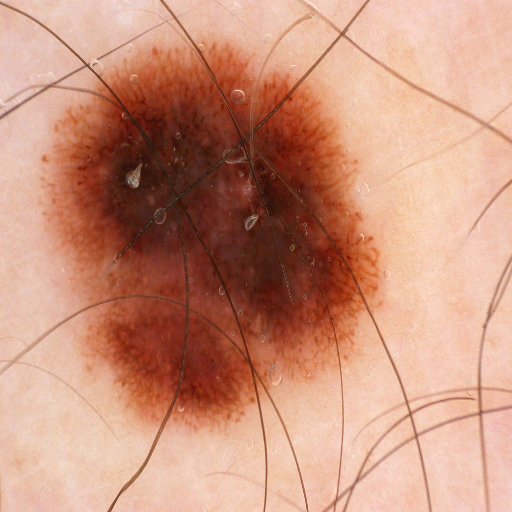
\includegraphics[width=\textwidth,keepaspectratio]{images/background/dermoscopic_sample.png}
		\caption{Dermoscopic image.}
		\label{fig:dermo-sample}
	\end{subfigure}
	\hfill
	\begin{subfigure}[b]{0.3\textwidth}
		\centering
		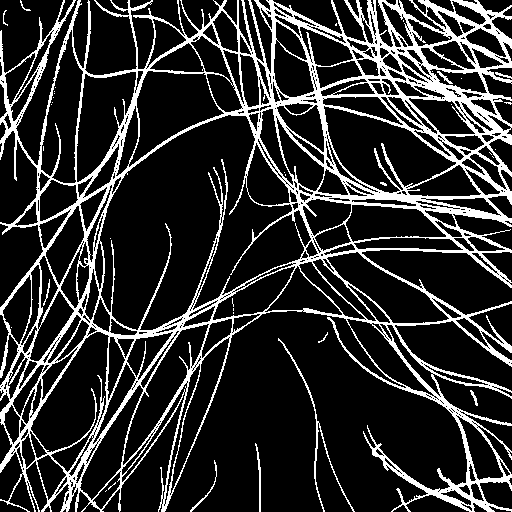
\includegraphics[width=\textwidth,keepaspectratio]{images/background/hair_mask_sample.png}
		\caption{Skin lesion hair mask.}
		\label{fig:hair-mask-sample}
	\end{subfigure}
	
	\caption[Clinical image vs dermoscopic image and a sample of skin lesion hair mask.]{Clinical image of erythema migrans \cite{EMPatterns} vs demoscopic image of skin cancer \cite{Tschandl2018} and a sample of skin lesion hair mask.}
	\label{fig:clinical-vs-dermo}
\end{figure}


Incorporating data from multiple modalities in the analysis process significantly improves the models' performance for skin lesion analysis tasks. For some diseases like Lyme disease, a proper diagnosis based on skin lesions is not effective without considering additional context from patient data. Existing works on early Lyme disease prediction using artificial intelligence techniques only utilize images of EM skin lesions whereas doctors believe corresponding patient data should also be considered to strengthen the predictive performance \cite{Burlina2020,Hossain2022}. Training a multimodal deep learning model utilizing both images and patient data requires a dataset of lesion images with associated patient data. Even though EM image datasets are available, creating a dataset with patient data linked with each lesion image would take much time. Moreover, patient data-only datasets that can be used for creating individual classifiers for Lyme disease are not readily available. So, our second research question is:
%\begin{tcolorbox}[width=\textwidth]    
\begin{researchquestion}\label{question2}
	How to assist deep learning based skin lesion image classifier with patient data in the absence of training data?
\end{researchquestion}
%\end{tcolorbox} 

Occlusion of skin lesions in dermoscopic images due to hair artifacts (as shown in Figure \ref{fig:dermo-sample}) affects the performance of computer-assisted lesion analysis algorithms. To tackle this issue, researchers are working on digital hair segmentation, removal, and augmentation techniques \cite{Attia2020,Li2021}. Standard image processing based hair removal is not beneficial for real-time application and removing hair does not give new features to the network. Augmenting images with skin hair can be of interest. Skin hair augmentation techniques require a hair mask to generate hair in given locations as shown in Figure \ref{fig:hair-mask-sample} \cite{Attia2020}. These masks are created either manually, with random curves or lines and segmentation \cite{Attia2020}. Generative models can be utilized to automate the creation of hair masks. So, our third research question is:
%\begin{tcolorbox}[width=\textwidth]  
\begin{researchquestion}\label{question3}
	How to efficiently deal with skin lesion hair artifacts for AI-assisted analysis of dermoscopic skin lesion images?
\end{researchquestion}
%\end{tcolorbox} 

\section{Conclusion}
%%%%%%%%%%%%%%%%%%%%%%%%%%%%%%%%%%%%%%%%%%%%%%%%%%%%%%%%%%%%%%%%%%%%%%%%
In this chapter, we have provided all the theoretical backgrounds needed to understand the rest of the thesis. In addition, we presented a detailed review of existing works in the literature and framed our research questions in the context of existing works. The following chapters describe our contributions by addressing the research questions presented in this chapter. 
\begin{tcolorbox}[enhanced,attach boxed title to top center={yshift=-3mm,yshifttext=-1mm},
	coltitle=black, colback=blue!5!white,colframe=blue!75!black,colbacktitle=violet!50!white,
	title=Key Points (Chapter \ref{chap:background}),fonttitle=\bfseries,
	boxed title style={colframe=black} ]
	In this thesis, we are addressing three research questions:
	\begin{itemize}
		\item Can we improve the performance of ImageNet pretrained clinical skin lesion image classifier's performance with additional pre-training using dermoscopic images?
		\item How to assist deep learning based skin lesion image classifier with patient data in the absence of training data?
		\item How to efficiently deal with skin lesion hair artifacts for AI-assisted analysis of dermoscopic skin lesion images?
	\end{itemize}
\end{tcolorbox}

	%%%%%%%%%%%%%%%%%%%%%%%%%%%%%%%%%%%%%%%%%%%%%%%%%%%%%%%%%%%%%%%%%%%%%%%%
\chapter{Pre-training Strategy for Improving Clinical Skin Lesion Image Classifier's Performance Using Dermoscopic Images}\label{chap:Pretraining}\chaptermark{Pre-training Strategy}
%%%%%%%%%%%%%%%%%%%%%%%%%%%%%%%%%%%%%%%%%%%%%%%%%%%%%%%%%%%%%%%%%%%%%%%%

\begin{center}
	\begin{minipage}{0.8\textwidth}
		\begin{small}
			This chapter addresses research question \ref{question1}, presents our pre-training strategy for improving clinical skin lesion image classification performance of ImageNet pre-trained convolutional neural networks by utilizing additional pre-training with dermoscopic images. It also contains benchmarking of state-of-the-art convolutional architectures for Lyme disease image classification. Contents from this chapter have been used in the following article:
			\begin{itemize}
				\item \fullcite{Hossain2022}
			\end{itemize}  
		\end{small}
	\end{minipage}
	\vspace{0.5cm}
\end{center}

\minitoc

%%%%%%%%%%%%%%%%%%%%%%%%%%%%%%%%%%%%%%%%%%%%%%%%%%%%%%%%%%%%%%%%%%%%%%%%
\section{Introduction}
%%%%%%%%%%%%%%%%%%%%%%%%%%%%%%%%%%%%%%%%%%%%%%%%%%%%%%%%%%%%%%%%%%%%%%%%
%\begin{table}
%	\caption{A stunning table}
%	\label{tbl:excel-table}
%	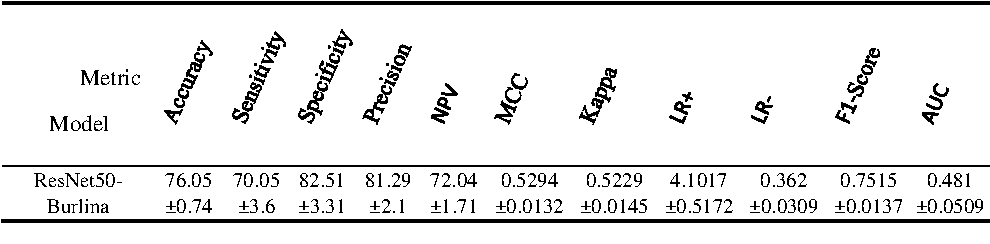
\includegraphics[width=\linewidth]{images/pretraining/ResNet50Table-cropped.pdf}
%\end{table}
Our pre-training strategy involves fine-tuning some layers from the end of an ImageNet pre-trained convolutional neural network (CNN) architecture using a dermoscopic dataset before training the model on a clinical skin lesion dataset. Our intuition behind the approach is the fact that even though the image modality of dermoscopic and clinical skin lesion images are different, pre-training some layers from the end of the model with dermoscopic images should provide a good feature representation for starting training with clinical skin lesion images. As the layers at the end of a CNN architecture respond to task-specific complex patterns, there should be a similarity between the skin lesion patterns of clinical and dermoscopic skin lesion images. We tested our strategy using dermoscopic images of skin cancer from HAM10000 dataset \cite{Tschandl2018} and clinical skin lesion images related to erythema migrans (EM).


As there is no expert-verified publicly available Lyme dataset of EM images, first, we created a dataset consisting of 866 images of confirmed EM lesions. Images collected from the internet and Clermont-Ferrand University Hospital Center (CF-CHU) of France were carefully labeled into two classes: EM and Confuser, by expert dermatologists and infectiologists from CF-CHU. CF-CHU collected the images from several hospitals in France.

Lightweight CNN-based mobile applications can help people with an initial self-assessment of EM and refer them to expert dermatologist for further diagnosis. Also, resource-intensive CNN-based computer applications can assist non-expert practitioners in identifying EM. In this chapter, besides testing our pre-training strategy, we also studied the performance of state-of-the-art CNNs for diagnosing Lyme disease from EM images and to find out the best architecture based on different criteria. We benchmarked twenty-five well-known CNNs on the prepared dataset in terms of several predictive performance metrics, computational complexity metrics, and statistical significance tests. Alongside our proposed pre-training strategy other best practices for training CNNs on limited data were used. For visualizing the regions of the input image that are significant for predictions from the CNN models we used gradient-weighted class activation mapping (Grad-CAM) \cite{Selvaraju2020}. We provided guidelines for model selection based on predictive performance and computational complexity. Moreover, we made all the trained models publicly available which can be used for transfer learning and building pre-scanners for Lyme disease. Figure \ref{fig:visualization-benchmark} presents the graphical overview of the study performed in this chapter.

The rest of the chapter is structured as follows: Section \ref{sec:matandmeth} contains the proposed pre-training strategy, dataset description, a brief overview of CNN architectures, and performance measures; Section \ref{sec:exp_result_pretrain} presents experimental studies, results, discussion, and recommendations for model selections; finally, Section \ref{sec:concluion_pretrain} presents concluding remarks.
%%%%%%%%%%%%%%%TO-DO%%%%%%%%%%%%%%%%%%%%%
\begin{figure}[htb!]
	\centering
	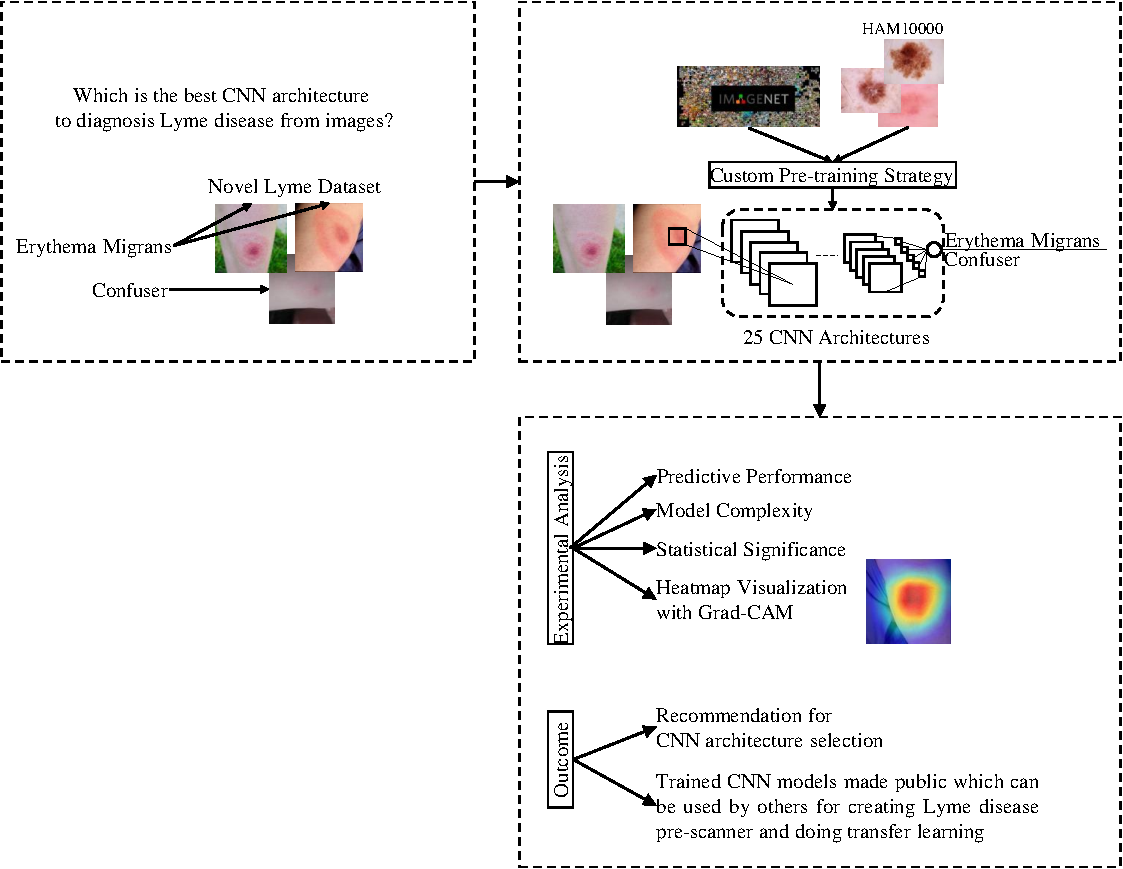
\includegraphics[width=\textwidth,keepaspectratio]{images/pretraining/Visualization-cropped.pdf}
	\caption{Graphical overview of the study on the effectiveness of CNNs utilizing custom pre-training strategy for the diagnosis of Lyme disease from images.}
	\label{fig:visualization-benchmark}
\end{figure}
%%%%%%%%%%%%%%%%%%%%%%%%%%%%%%%%%%%%%%%%%%%%%%%%%%%%%%%%%%%%%%%%%%%%%%%%
\section{Materials and Methods}\label{sec:matandmeth}
%%%%%%%%%%%%%%%%%%%%%%%%%%%%%%%%%%%%%%%%%%%%%%%%%%%%%%%%%%%%%%%%%%%%%%%%
The following subsections describe the pre-training strategy used in this study, the data organization, a short overview of the considered CNN architectures, performance measures, and heatmap visualization method.
%%%%%%%%%%%%%%%%%%%%%%%%%%%%%%%%%%%%%%%%%%%%%%%%%%%%%%%%%%%%%%%%%%%%%%%%
\subsection{Pre-training Strategy}\label{sec:pretraining-strag}
%%%%%%%%%%%%%%%%%%%%%%%%%%%%%%%%%%%%%%%%%%%%%%%%%%%%%%%%%%%%%%%%%%%%%%%%
\SetAlFnt{\small}
%\SetAlCapFnt{\t}
%\SetAlCapNameFnt{\large}
\SetKwProg{Fn}{Function}{}{}
\begin{algorithm}[htb!]
	\DontPrintSemicolon
	\SetKwFunction{findLayersToUnfreeze}{findLayersToUnfreeze}
	\SetKwInOut{KwIn}{Data}
	\SetKwInOut{KwOut}{Output}
	
	\KwIn{\newline ImageNet pre-trained CNN model without classfication head: $M_{I}$\newline
		Total layers in $M_{I}$: $N_{L}$\newline
		Dermoscopic image classification task: $\mathcal{T}_{S}$\newline
		Dermoscopic image dataset: $D_{S}$\newline
		Clinical skin lesion image classification task: $\mathcal{T}_{T}$\newline
		Clinical skin lesion image dataset: $D_{T}$\newline
	}
	
	\KwOut{\newline CNN model optimized for $\mathcal{T}_{T}: M_{T}$}
	
	\Begin{
		$M_{I} \gets$ freeze all the layers of $M_{I}$\tcp*[f]{make layers non-trainable}\;
		$U_{L} \gets$ findLayersToUnfreeze($M_{I}$, $N_{L}$, $\mathcal{T}_{T}$, $D_{T}$)\;
		$M_{S} \gets$ add classifier head to $M_{I}$ for $\mathcal{T}_{S}$\;
		\tcc{models are trained and validated using training and validation subsets of the respective dataset}
		$M_{S} \gets$ train $M_{S}$ and fine-tune after unfreezing layers $N_{L}-U_{L}+1$ to $N_{L}$ on $D_{S}$\;
		$M_{S} \gets$ freeze all the layers of $M_{S}$\;
		$M_{T} \gets$ from $M_{S}$ remove classifier head for $\mathcal{T}_{S}$ and add classifier head for $\mathcal{T}_{T}$\;
		$M_{T} \gets$ train $M_{T}$ and fine-tune after unfreezing layers $N_{L}-U_{L}+1$ to $N_{L}$ on $D_{T}$\;
		\KwRet{$M_{T}$}
	}	
	
	\Fn{findLayersToUnfreeze ($M$, $N$, $\mathcal{T}$, $D$)}{
		$M_{T} \gets$ add classifier head to $M$ for $\mathcal{T}$\;
		$\tilde{M}_{T} \gets$ train $M_{\mathcal{T}}$ using training data from $D$\;
		$U \gets 0$ \tcp*[f]{number of layers to unfreeze}\;
		$max \gets 0$ \tcp*[f]{tracks best model accuracy on validation data}\;
		\For{$i \gets 1$ \textbf{to} $N$} {
			$M_{T} \gets$ unfreeze layers $N-i+1$ to $N$ of  $M_{T}$\tcp*[f]{make  layers trainable}\; 
			$M_{T} \gets$ fine-tune $M_{T}$ using training data from $D$\;
			$temp \gets$ measure accuracy of $M_{T}$ on validation data from $D$\;
			\If{$temp > max$} {
				$max \gets temp$\;
				$U \gets i$\;
			}   
			$M_{T} \gets \tilde{M}_{T}$\;
		}
		
		\KwRet{$U$}
	}
	
	\caption{Dermoscopic pre-training for clinical lesion image classification}
	\label{algo:pretraining}	
\end{algorithm}
Algorithm \ref{algo:pretraining} shows the steps of our pre-training strategy. We start with an ImageNet pre-trained CNN model $M_{I}$ without the original ImageNet classification head. The total layers in $M_{I}$ is $N_{L}$. The source dermoscopic image classification task and dataset are $\mathcal{T}_{S}$, and $D_{S}$, respectively. The target clinical skin lesion image classification task and dataset are $\mathcal{T}_{T}$, and $D_{T}$, respectively. Initially, all the layers of $M_{I}$ are frozen to make sure the parameters are not updated during training. Then, we find out the best number of layers $U_{L}$ of $M_{I}$ to unfreeze and fine-tune for  $\mathcal{T}_{T}$ using the function \textit{findLayersToUnfreeze}. The function first adds a classification head to $M_{I}$ for $\mathcal{T}_{T}$ and trains the model using $D_{T}$. Then, the function trains the model by making different frozen layers trainable and the number of unfrozen layers giving the best validation accuracy is returned. $M_{I}$ is again pre-trained and fine-tuned using $D_{S}$ based on $U_{L}$. For that purpose, we add classification head to  $M_{I}$  for $\mathcal{T}_{S}$ resulting in a model called $M_{S}$. $M_{S}$ is trained and fine-tuned after unfreezing layers $N_{L}-U_{L}+1$ to $N_{L}$ using $D_{S}$. Then all the layers of $M_{S}$ are made non-trainable again. After pre-training and fine-tuning the unfrozen part of the model for $\mathcal{T}_{S}$, the learned feature representation is reused for $\mathcal{T}_{T}$. We remove the classifier head for $\mathcal{T}_{S}$ from $M_{S}$ and add the classifier head for $\mathcal{T}_{T}$ resulting in a model called $M_{T}$. Finally, $M_{T}$ is trained and fine-tuned after unfreezing layers $N_{L}-U_{L}+1$ to $N_{L}$ using $D_{S}$. We tested the proposed pre-training strategy on EM classification task as shown in Figure \ref{fig:pre-training}. The source dermoscopic image classification task $\mathcal{T}_{S}$ and dataset $D_{S}$ are skin cancer classification and HAM10000 dataset respectively. The target clinical skin lesion image classification task $\mathcal{T}_{T}$ and dataset $D_{T}$ are EM classification and Lyme dataset respectively. Our EM classification head consists of global average pooling (GAP) layer \cite{Lin2014}, dropout layer \cite{Srivastava2014}, and a fully connected layer with sigmoid activation for binary classification. Each channel in the feature map is averaged over the whole spatial extent by GAP, and the end result is a single value for each channel that summarizes the spatial information of the feature map. Dropout is a deep learning regularization method used to avoid overfitting. During each training iteration, a portion of the units or neurons in a layer are randomly dropped out (i.e., set to zero) by the dropout layer. As it can no longer rely on any one neuron, this forces the network to learn more reliable and generalizable features.
\begin{figure}[htb!]
	\centering
	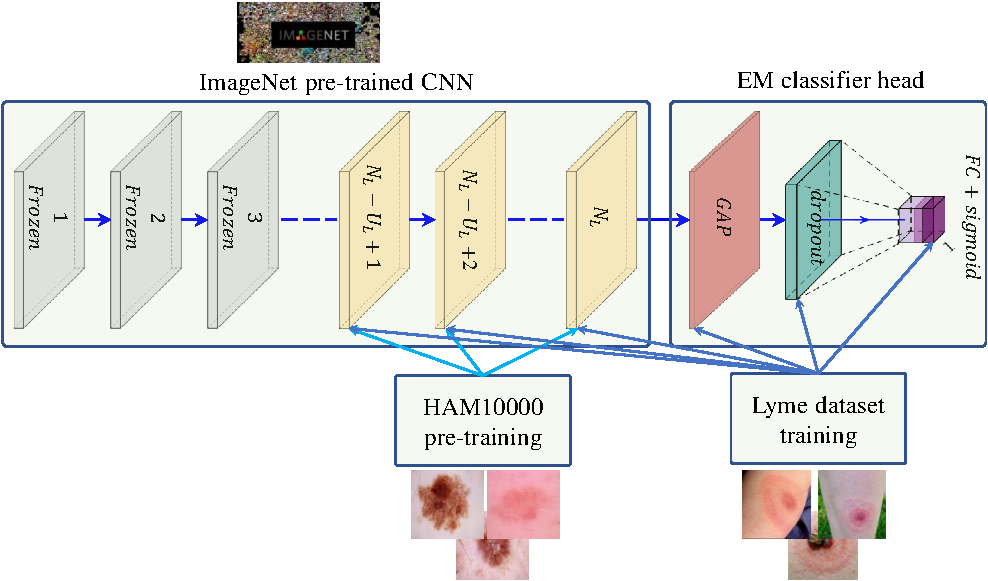
\includegraphics[width=\textwidth,keepaspectratio]{images/pretraining/pretraining-cropped.pdf}
	\caption[Pre-training strategy applied to erythema migrans  classification]{Pre-training strategy applied to erythema migrans (EM) classification. $GAP$ and $FC$ stand for global average pooling and fully connected layer respectively. $N_{L}$ is the number of ImageNet pre-trained layers and $U_{L}$ represents the number of layers used for fine-tuning. }
	\label{fig:pre-training}
\end{figure}

The intuition behind our approach is the fact that CNN mimics the ventral visual stream process of the human brain \cite{Zhuang2021}. Figure \ref{fig:ventral-stream} shows the outline of the ventral visual stream. The first visual area V1 receives optical input from the retina through the optic nerve and the lateral geniculate nucleus. V1 responds to very simple patterns (edges, lines). As the input traverses through the stream V2 and V4 respond to simple and complex shapes respectively. Further down the path inferotemporal areas respond to complex patterns of semantic entities for object understanding \cite{Qin2018}. CNNs replicate the behavior of the ventral visual stream. The initial layers of CNN learn/respond to simple patterns and the later layers respond to complex and semantic patterns. The unfrozen layers at the end of ImageNet pre-trained model giving good performance when fine-tuned on clinical skin lesion image dataset learn task-specific patterns that relate to clinical skin lesions and there should be a similarity between the skin lesion patterns of clinical and dermoscopic skin lesion images. So, fine-tuning the unfrozen part first with a dermoscopic image dataset should provide a good feature representation and weight initialization of layers for starting training with a clinical skin lesion image dataset.    
\begin{figure}[htb!]
	\centering
	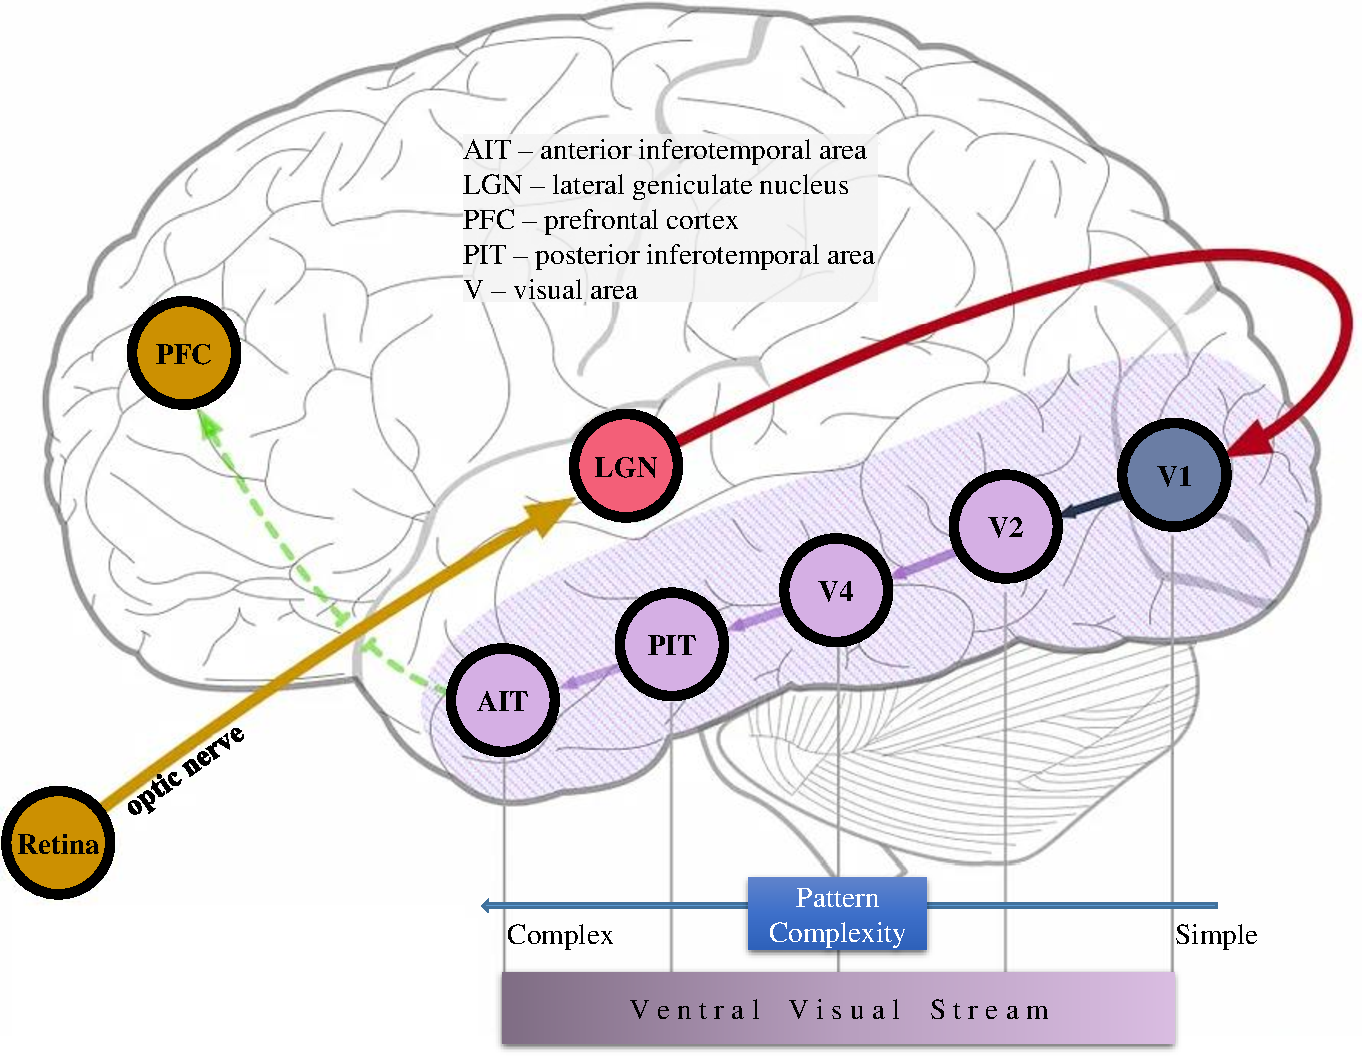
\includegraphics[width=\textwidth,keepaspectratio]{images/pretraining/ventral-stream-cropped.pdf}
	\caption[Outline of ventral visual stream]{Outline of ventral visual stream. Image modified from \cite{ventral-system}.}
	\label{fig:ventral-stream}
\end{figure}

%%%%%%%%%%%%%%%%%%%%%%%%%%%%%%%%%%%%%%%%%%%%%%%%%%%%%%%%%%%%%%%%%%%%%%%%
\subsection{Dataset Preparation}\label{sec:dataset_prep}
%%%%%%%%%%%%%%%%%%%%%%%%%%%%%%%%%%%%%%%%%%%%%%%%%%%%%%%%%%%%%%%%%%%%%%%%

As a labeled public dataset is not available for Lyme disease prediction from EM images, we created a dataset by collecting clinical skin lesion images from the internet and CF-CHU. CF-CHU collected EM images from several hospitals located in France. The use of images from the internet was inspired by related skin lesion analysis studies \cite{Burlina2018, Burlina2020, Esteva2017}. Duplicate images were removed using an image hashing-based duplicate image detector followed by the removal of inappropriate images through human inspection. After the initial curation steps, we got a total of 1672 images. Expert dermatologists and infectiologists from CF-CHU classified the curated images into two categories: EM and Confuser, making it a two-class classification problem. Out of 1672 images, 866 images were assigned to EM class and 806 images were assigned to Confuser class. The images collected from the hospitals are not shareable because of the confidentiality agreement signed with the patients. We can share images collected from the internet and the corresponding labels assigned by the doctors subject to an agreement that the images will not be made public because we do not have permission from the owners of the images \footnote{Interested researchers can send a request to dappem-project@inrae.fr for the data.}.

We further subdivided the dataset into five folds using stratified five-fold cross-validation to make sure each of the folds maintains the original class ratio. One of the folds was used as a test set and the remaining four were used as the training set with a rotation of the folds for five runs. Each time, 10\% of the training data was assigned to the validation set as shown in Figure \ref{fig:cross-validation}.
\begin{figure}[htb!]
	\centering
	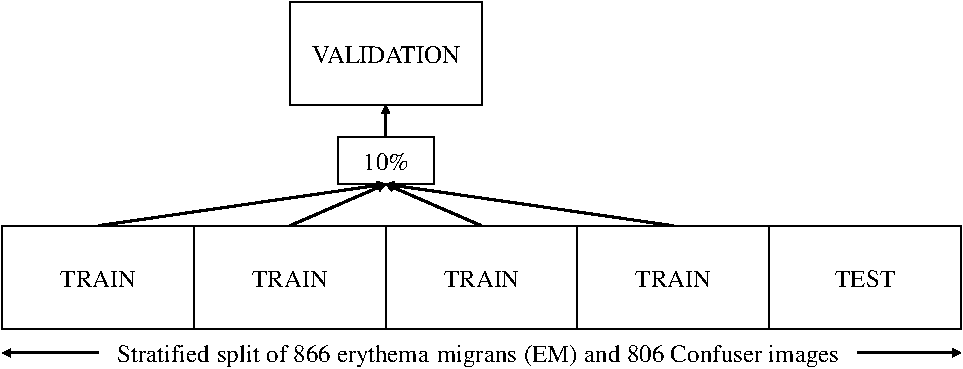
\includegraphics[width=\textwidth,keepaspectratio]{images/pretraining/cross-validation-cropped.pdf}
	\caption[Five-fold cross-validation setup]{Five-fold cross-validation setup.}
	\label{fig:cross-validation}
\end{figure}

Deep CNNs require a considerable amount of data for training and data augmentation can help with expanding the dataset. We applied data augmentation techniques only to the training images. We used flip (vertical or horizontal), rotation, brightness, contrast, and saturation augmentation by considering the best performing augmentations for skin lesions \cite{Perez2018}. Besides, we also used perspective skew transformation to cover the case of looking at a picture from different angles. Augmentor \cite{Bloice2019} an image augmentation library specially built for biomedical image augmentation was used for applying the augmentations. We used 0.5 as the probability of applying each of the augmentation operations. Rotation operation was performed with a maximum rotation angle of 5 degrees. We also used random rotation by either 90, 180, or 270 degrees. Brightness, contrast, and saturation augmentations were performed with a minimum adjustment factor of 0.7 and a maximum adjustment factor of 1.3. For all the other parameters we used default values provided by Augmentor library. The parameters were adjusted based on the visual inspection of augmented images. Figure \ref{fig:augmentation} shows some example images resulting from augmentations applied on a sample image.

\begin{figure}[htb!]
	\centering
	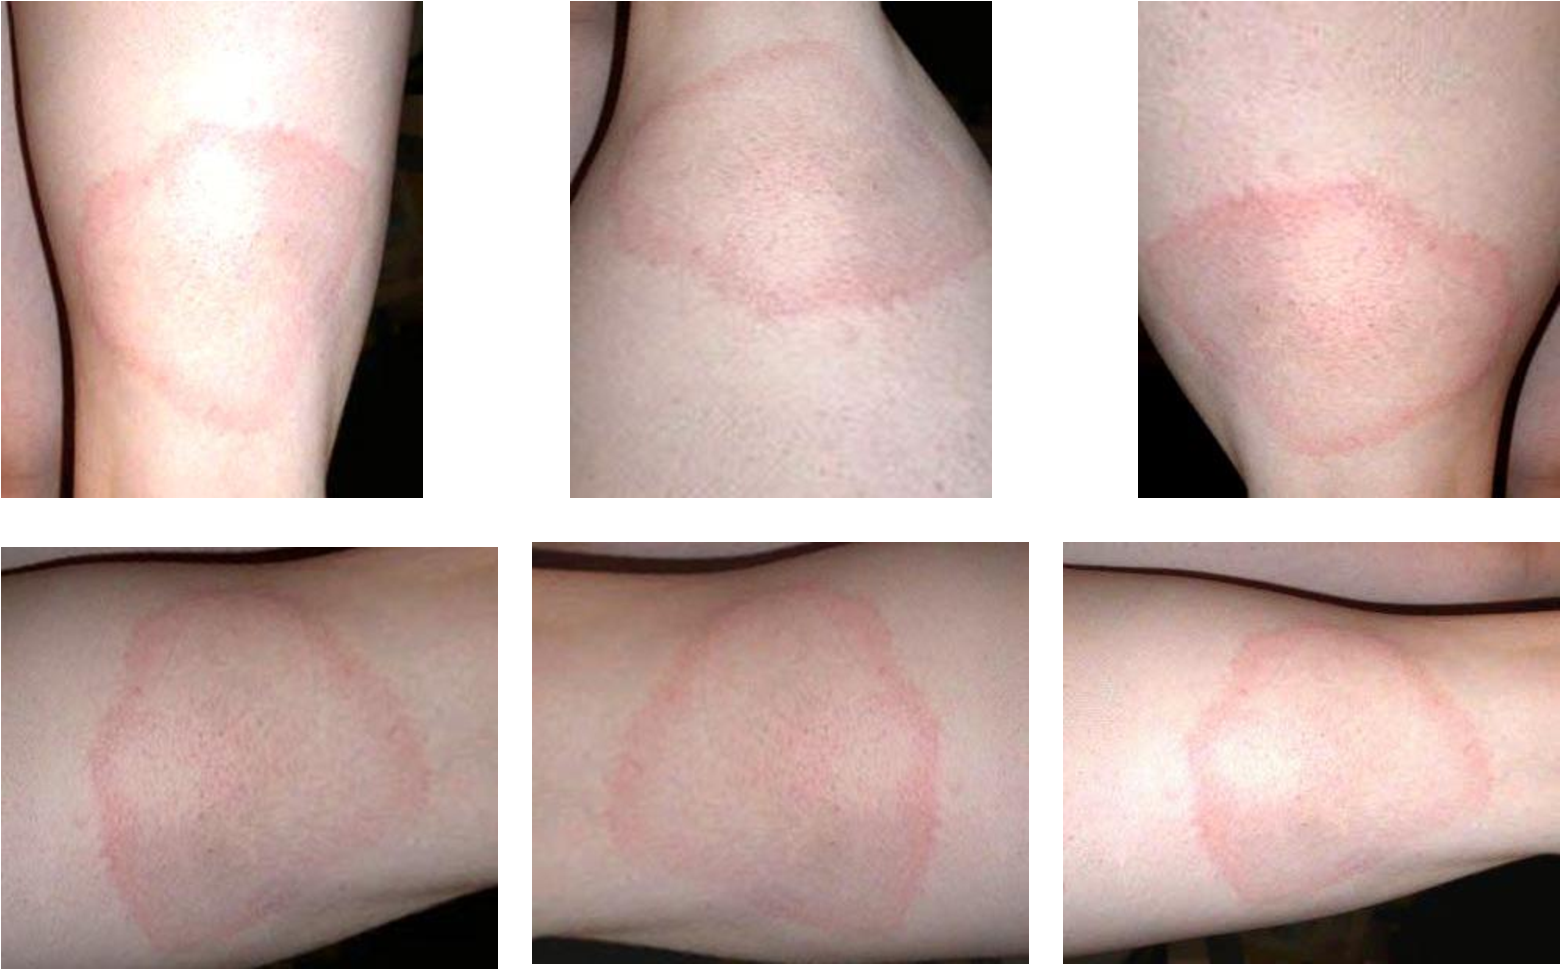
\includegraphics[width=\textwidth,keepaspectratio]{images/pretraining/Augmentation-cropped.pdf}
	\caption[Data augmentation examples]{Data augmentation examples.}
	\label{fig:augmentation}
\end{figure}

%%%%%%%%%%%%%%%%%%%%%%%%%%%%%%%%%%%%%%%%%%%%%%%%%%%%%%%%%%%%%%%%%%%%%%%%
\subsection{Brief Overview of the CNN Architectures Considered in the Study}\label{sec:CNN-archis}
%%%%%%%%%%%%%%%%%%%%%%%%%%%%%%%%%%%%%%%%%%%%%%%%%%%%%%%%%%%%%%%%%%%%%%%%
Starting with LeNet \cite{726791} in 1988 the popularity of CNNs increased with AlexNet \cite{Krizhevsky2017} winning the ImageNet large scale visual recognition challenge (ILSVRC) \cite{Russakovsky2015} of 2012. As a result of the effectiveness of CNNs in solving complex problems, several CNN architectures have been introduced over the past few years. The following subsections provide a brief overview of the CNN architectures used in this study.

%%%%%%%%%%%%%%%%%%%%%%%%%%%%%%%%%%%%%%%%%%%%%%%%%%%%%%%%%%%%%%%%%%%%%%%%
\subsubsection{VGG Architecture}
%%%%%%%%%%%%%%%%%%%%%%%%%%%%%%%%%%%%%%%%%%%%%%%%%%%%%%%%%%%%%%%%%%%%%%%%
VGG architecture \cite{Simonyan2015} is based on the idea of deeper networks with smaller filters $\left(3\times3\right)$. There are thirteen convolutional layers and three fully connected layers in VGG16 architecture as shown in Figure \ref{fig:VGG16}. Another variation of VGG architecture called VGG19 has sixteen convolutional layers and three fully connected layers. VGG architecture showed better effectiveness of deeper architectures in terms of predictive performance but requires training a huge number of parameters. 
\begin{figure}[htb!]
	\centering
	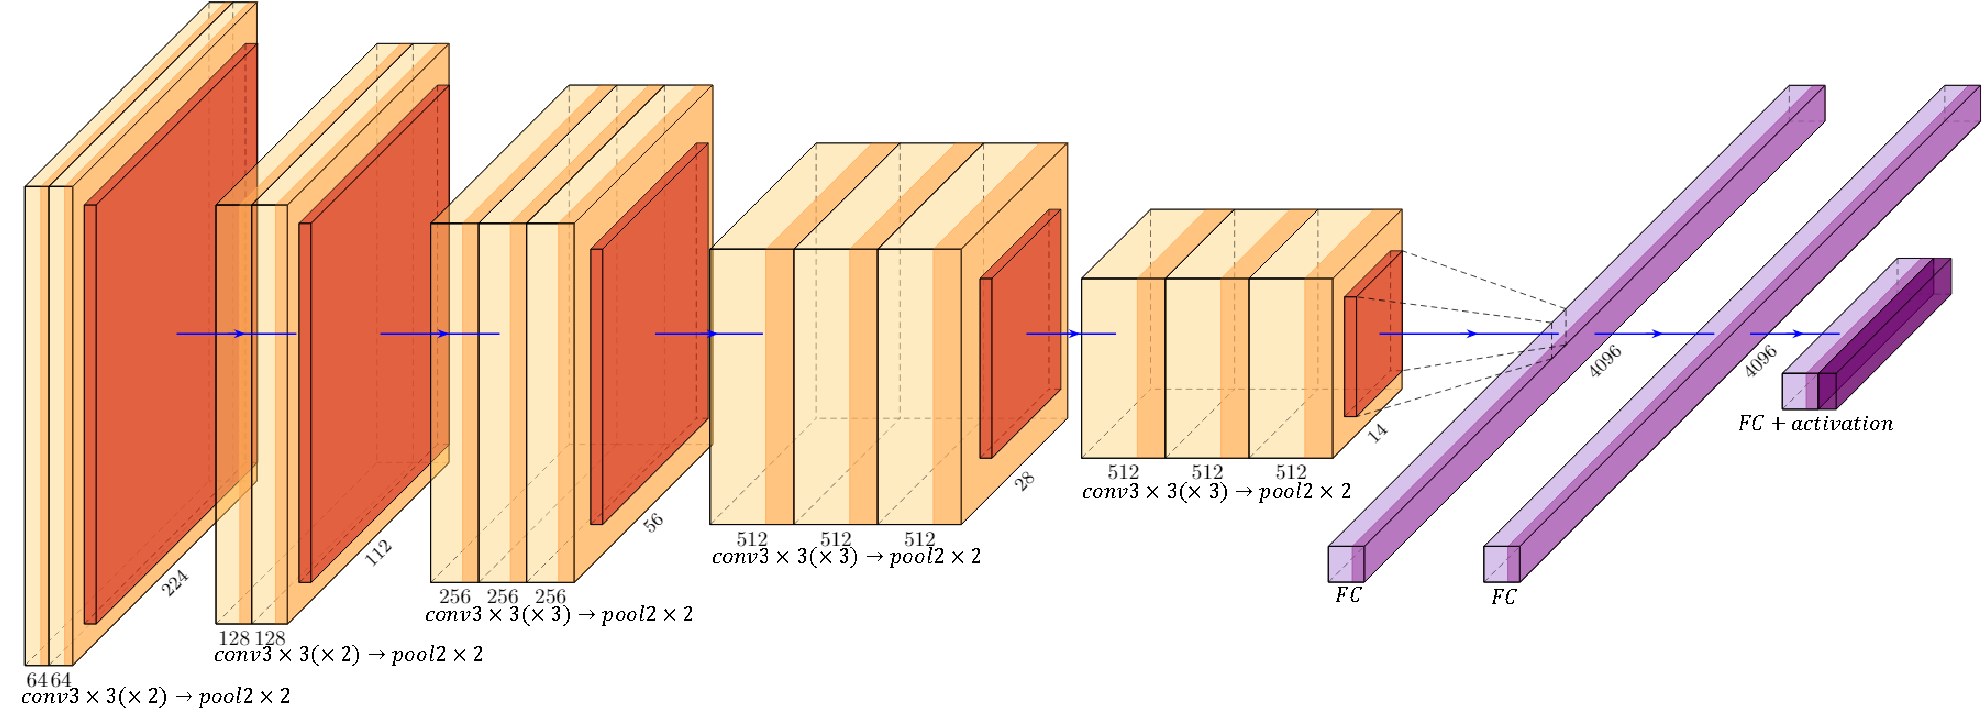
\includegraphics[width=\textwidth,keepaspectratio]{images/pretraining/VGG-cropped.pdf}
	\caption[VGG16 architecture]{VGG16 architecture. Input image is of shape $224\times224\times3$. $FC$ stands for fully connected layer.}
	\label{fig:VGG16}
\end{figure}

%%%%%%%%%%%%%%%%%%%%%%%%%%%%%%%%%%%%%%%%%%%%%%%%%%%%%%%%%%%%%%%%%%%%%%%%
\subsubsection{Inception Architecture}
%%%%%%%%%%%%%%%%%%%%%%%%%%%%%%%%%%%%%%%%%%%%%%%%%%%%%%%%%%%%%%%%%%%%%%%%
Inception architecture \cite{Szegedy2015} uses inception module as shown in Figure \ref{fig:Inception}, which is a combination of several convolution layers with small filters $\left ( 1\times1,\,3\times3,\,5\times5\right )$ applied simultaneously on the same input to facilitate the extraction of more information. The output filter banks from the convolution layers of inception module are concatenated into a single vector, which is served as the input for next stage. To reduce learnable parameters and computational complexity inception module uses $1\times1$ convolution at the beginning of convolution layers. InceptionV1 architecture is the winner of ILSVRC 2014 competition, and it’s also known as GoogleNet. Further improvement resulted in the creation of several versions of inception architectures named InceptionV2, InceptionV3, and InceptionV4 \cite{Szegedy2016, Szegedy2017}.  InceptionV2 and InceptionV3 improved the architecture with smart factorized convolution, batch normalized auxiliary classifier, and label smoothing whereas, InceptionV4 focused on the uniformity of the architecture with more inception modules than InceptionV3.
\begin{figure}[htb!]
	\centering
	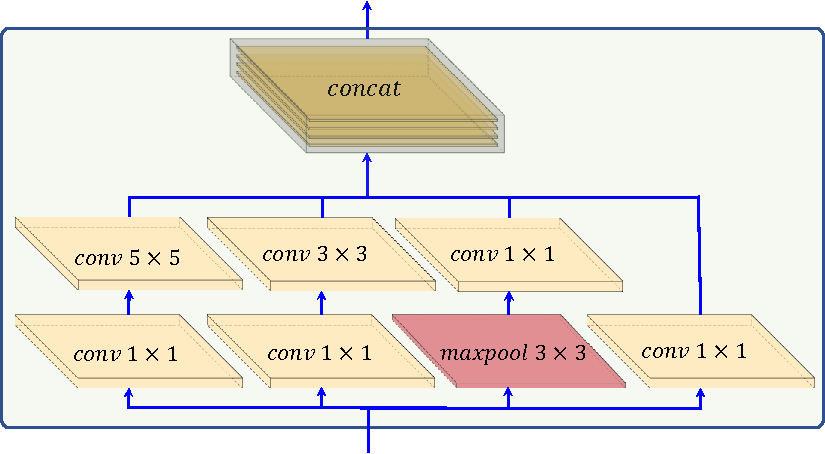
\includegraphics[width=\textwidth,keepaspectratio]{images/pretraining/Inception-cropped.pdf}
	\caption[Inception module of Inception architecture]{Inception module of Inception architecture. \enquote{concat} represents the concatenation of feature maps.}
	\label{fig:Inception}
\end{figure}

%%%%%%%%%%%%%%%%%%%%%%%%%%%%%%%%%%%%%%%%%%%%%%%%%%%%%%%%%%%%%%%%%%%%%%%%
\subsubsection{ResNet Architecture}
%%%%%%%%%%%%%%%%%%%%%%%%%%%%%%%%%%%%%%%%%%%%%%%%%%%%%%%%%%%%%%%%%%%%%%%%
ResNet architecture \cite{He2016} tried to solve the vanishing gradient and accuracy degradation problems of deep models by introducing residual block with identity shortcut connection that directly connects the input to the output of the block allowing the gradient to flow through the shortcut path as shown in Figure \ref{fig:resnet}. It’s the winner of ILSVRC 2015 competition. Depending on the number of weight layers there are many variants of ResNet architecture such as ResNet18, ResNet34, ResNet50, ResNet101, ResNet152, ResNet164, ResNet1202, etc., where the number represents the count of weight layers. Deeper ResNet architectures use bottleneck blocks where 3x3 convolution is sandwiched between $1\times1$ convolutions, responsible for transitory reduction and expansion of channels.  The $wide\rightarrow narrow \rightarrow wide$ architecture of bottlenecks reduces multiplications and the number of parameters and helps the network grow deeper with fewer parameters. He et al. \cite{He2016a} proposed ResNetV2 with pre-activation of the weight layers as opposed to the post-activation of original ResNet architecture.  InceptionResNet is a hybrid of Inception and ResNet architecture having two variations named InceptionResNetV1 and InceptionResNetV2, which differ mainly in terms of the number of used filters \cite{Szegedy2017}. Liu et al. \cite{ConvNeXtRef} modernized ResNet architecture to match the performance of vision transformers resulting in a new family of architectures called ConvNeXt. ConvNeXt utilizes inverted bottleneck ( $narrow\rightarrow wide \rightarrow narrow$), large kernel, depthwise convolution (shown in Figure \ref{fig:depthwise}), layer normalization \cite{LayerNormRef} instead of batch normalization \cite{BatchNormref}, and GELU activation ReLU as compared to base ResNet models.
\begin{figure}[htb!]
	\centering
	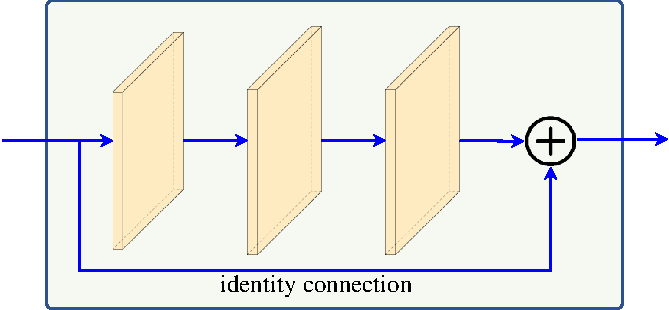
\includegraphics[width=0.5\textwidth,keepaspectratio]{images/pretraining/ResNet-cropped.pdf}
	\caption[Residual block of ResNet architecture]{Residual block of ResNet architecture.}
	\label{fig:resnet}
\end{figure}

%%%%%%%%%%%%%%%%%%%%%%%%%%%%%%%%%%%%%%%%%%%%%%%%%%%%%%%%%%%%%%%%%%%%%%%%
\subsubsection{DenseNet Architecture}
%%%%%%%%%%%%%%%%%%%%%%%%%%%%%%%%%%%%%%%%%%%%%%%%%%%%%%%%%%%%%%%%%%%%%%%%
Dense Convolutional Network (DenseNet) \cite{DenseNetRef} extended ResNet by introducing dense blocks where each layer within a dense block receives inputs from all the previous layers as shown in Figure \ref{fig:densenet} DenseNet concatenates the incoming feature maps of a layer with output feature maps instead of summing them up as done in ResNet. Dense blocks within DenseNet are connected with transition layers consisting of convolution and pooling to perform the required downsampling operation. Depending on the number of weight layers there are several versions of DenseNet like DenseNet121, DenseNet169, DenseNet201, DenseNet264, etc. Besides solving the vanishing gradient problem DenseNet also eases feature propagation and reuse, and a reduction in the number of learnable parameters compared to ResNet.
\begin{figure}[htb!]
	\centering
	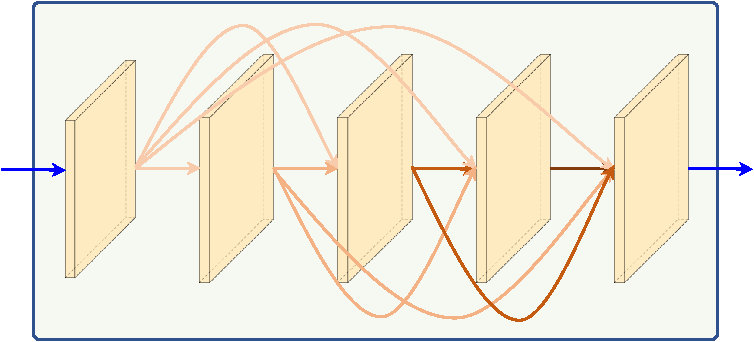
\includegraphics[width=0.6\textwidth,keepaspectratio]{images/pretraining/dense-cropped.pdf}
	\caption[Building block of DenseNet architecture]{Building block of DenseNet architecture.}
	\label{fig:densenet}
\end{figure}

%%%%%%%%%%%%%%%%%%%%%%%%%%%%%%%%%%%%%%%%%%%%%%%%%%%%%%%%%%%%%%%%%%%%%%%%
\subsubsection{MobileNet Architecture}
%%%%%%%%%%%%%%%%%%%%%%%%%%%%%%%%%%%%%%%%%%%%%%%%%%%%%%%%%%%%%%%%%%%%%%%%
MobileNetV1 \cite{Howard2017} used depthwise separable convolution extensively to reduce the computational cost. Standard convolution performs spatial and channel-wise computations in one step but depthwise separable convolution first applies separate convolutional filter for each input channel and then uses pointwise convolution on concatenated channels to produce required number of output channels as shown in Figure \ref{fig:depthwise}. MobileNetV1 was designed to run very efficiently on mobile and embedded devices. MobileNetV2 \cite{Sandler2018} improved upon the concepts of MobileNetV1 by incorporating thin linear bottlenecks with shortcut connections between the bottlenecks as shown in Figure \ref{fig:mobilenetv2}. This is called inverted residual block as it uses $narrow\rightarrow wide \rightarrow narrow$ as opposed to the $wide\rightarrow narrow \rightarrow wide$ architecture of traditional residual block. MobileNetV3 \cite{Howard2019} incorporated squeeze-and-excitation layers \cite{Hu2020} in the building block of MobileNetV2 which provides channel-wise attention and used MnasNet \cite{Tan2019} to search for a coarse architecture that was further optimized with NetAdapt \cite{Yang2018} algorithm.
\begin{figure}[htb!]
	\centering
	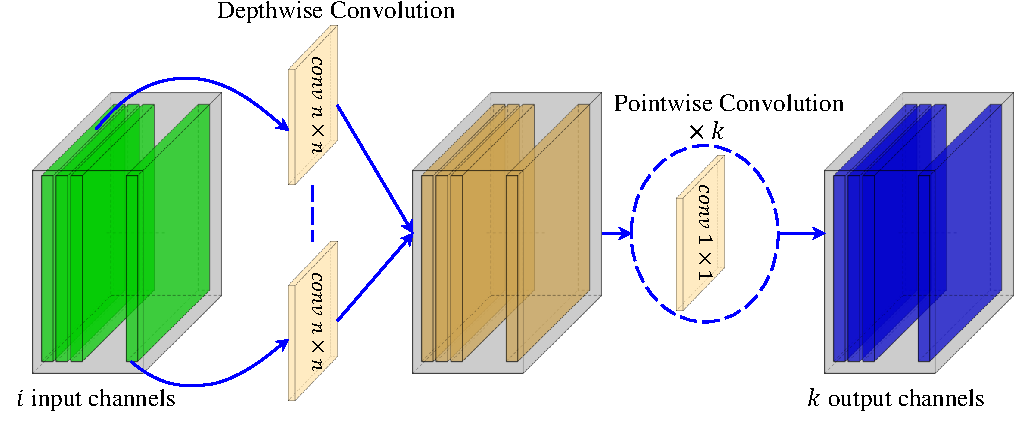
\includegraphics[width=\textwidth,keepaspectratio]{images/pretraining/depthwise-cropped.pdf}
	\caption[Depthwise separable convolution]{Depthwise separable convolution.}
	\label{fig:depthwise}
\end{figure}
\begin{figure}[htb!]
	\centering
	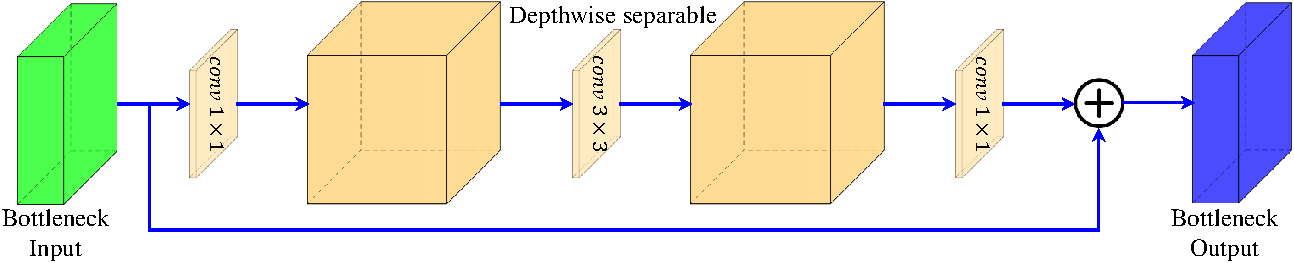
\includegraphics[width=\textwidth,keepaspectratio]{images/pretraining/mnetv2-cropped.pdf}
	\caption[Building block of MobileNetV2 architecture]{Building block of MobileNetV2 architecture.}
	\label{fig:mobilenetv2}
\end{figure}

%%%%%%%%%%%%%%%%%%%%%%%%%%%%%%%%%%%%%%%%%%%%%%%%%%%%%%%%%%%%%%%%%%%%%%%%
\subsubsection{Xception Architecture}
%%%%%%%%%%%%%%%%%%%%%%%%%%%%%%%%%%%%%%%%%%%%%%%%%%%%%%%%%%%%%%%%%%%%%%%%
Extreme version of Inception the Xception architecture \cite{XceptionRef} replaced the Inception module with a modified version of depthwise separable convolution where the order of depthwise convolution and pointwise convolutions are reversed as shown in Figure \ref{fig:xception}. Xception also uses shortcut connections like ResNet architecture. On ImageNet dataset Xception performs slightly better than the InceptionV3 architecture.
\begin{figure}[htb!]
	\centering
	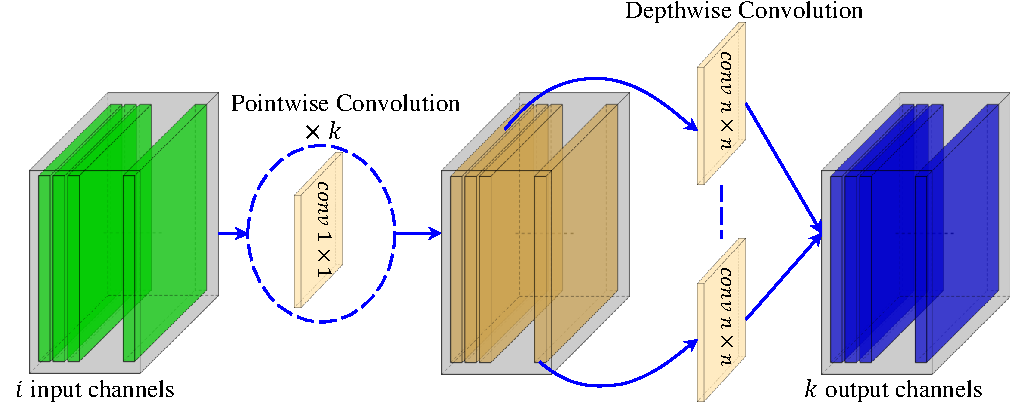
\includegraphics[width=\textwidth,keepaspectratio]{images/pretraining/pointwise-cropped.pdf}
	\caption[Building block of Xception architecture]{Building block of Xception architecture.}
	\label{fig:xception}
\end{figure}

%%%%%%%%%%%%%%%%%%%%%%%%%%%%%%%%%%%%%%%%%%%%%%%%%%%%%%%%%%%%%%%%%%%%%%%%
\subsubsection{NASNet Architecture}
%%%%%%%%%%%%%%%%%%%%%%%%%%%%%%%%%%%%%%%%%%%%%%%%%%%%%%%%%%%%%%%%%%%%%%%%
Neural Architecture Search Netowork \cite{NASnetref} from Google Brain utilizes reinforcement learning with a Recurrent Neural Network based controller to search for efficient building blocks for a smaller dataset which is then transferred to a larger dataset by stacking multiple copies of the found building block.  NASNet blocks are comprised of normal and reduction cells as shown in Figure \ref{fig:NASnet}. Normal cells produce feature maps of the same size as input whereas reduction cells reduce the size by a factor of two. NASNet optimized for mobile applications is called NASNetMobile whereas the larger version is called NASNetLarge.
\begin{figure}[htb!]
	\centering
	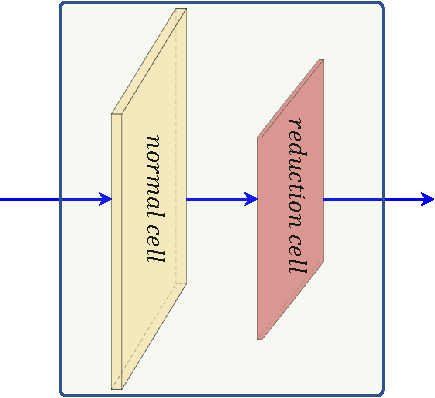
\includegraphics[width=0.4\textwidth,keepaspectratio]{images/pretraining/NASnet-cropped.pdf}
	\caption[Building block of NASNet architecture]{Building block of NASNet architecture.}
	\label{fig:NASnet}
\end{figure}

%%%%%%%%%%%%%%%%%%%%%%%%%%%%%%%%%%%%%%%%%%%%%%%%%%%%%%%%%%%%%%%%%%%%%%%%
\subsubsection{EfficientNet Architecture}
%%%%%%%%%%%%%%%%%%%%%%%%%%%%%%%%%%%%%%%%%%%%%%%%%%%%%%%%%%%%%%%%%%%%%%%%
EfficientNet \cite{efficientNetRef} which is among the most efficient models proposed a scaling method to uniformly scale all dimensions of a network using a compound coefficient. The baseline network of EfficientNet was built with NAS incorporating squeeze-and-excitation in the building block of MobileNetV2. EffcientNet’s building block also called MBConv is shown in Figure \ref{fig:MBConv}.
\begin{figure}[htb!]
	\centering
	\begin{subfigure}[b]{\textwidth}
		\centering
		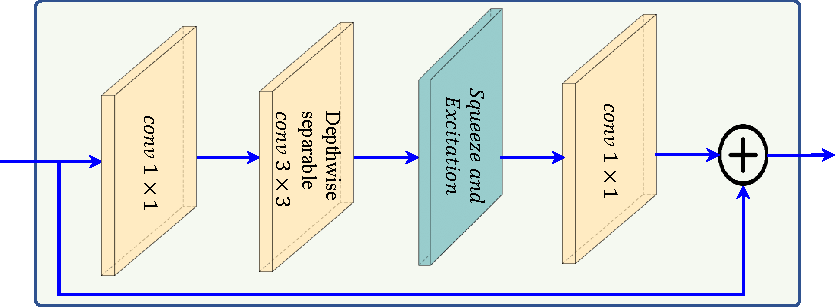
\includegraphics[width=\textwidth,keepaspectratio]{images/pretraining/MBConv-cropped.pdf}
		\caption{MBConv block.}
		\label{fig:MBConv}
	\end{subfigure}
	\hfill
	\begin{subfigure}[b]{0.75\textwidth}
		\centering
		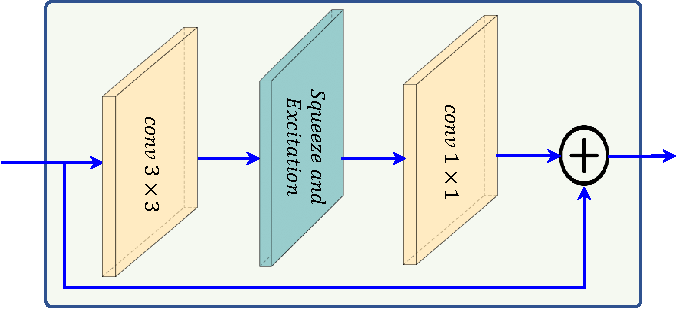
\includegraphics[width=\textwidth,keepaspectratio]{images/pretraining/FusedMBConv-cropped.pdf}
		\caption{Fused-MBConv block.}
		\label{fig:Fused-MBConv}
	\end{subfigure}
	
	\caption{EfficientNet building blocks.}
	\label{fig:mobilenet-blocks}
\end{figure}
The scaling method is defined as:
\begin{gather*}
	depth=\zeta_{1}^{\Theta}\\
	width=\zeta_{2}^{\Theta}\\
	resolution=\zeta_{3}^{\Theta}\\
	s.t.\; \zeta_{1}.\zeta_{2}^{2}.\zeta_{3}^{2}\approx2;\,\zeta_{1}\geq1,\zeta_{2}\geq1,\zeta_{1}\geq1
\end{gather*}
where, the coefficient $\Theta$ controls available resources and $\zeta_{1},\zeta_{2}$, and $\zeta_{3}$ are constants obtained by grid search. EfficientNetB0-B7 are a family of architectures scaled up from the baseline network that reflects a good balance of accuracy and efficiency. EfficientV2 was designed to optimize parameter efficiency and training speed. It used an additional Fused-MBConv block. Fused-MBConv uses $3\times3$ convolution instead of the $3\times3$ depthwise and $1\times1$ convolutions of MBConv as shown in Figure \ref{fig:Fused-MBConv}. Although Fused-MBConv adds a small overhead it improves training speed compared to MBConv. EfficientV2 used training-aware NAS to find the best combination of MBConv and Fused-MBConv blocks. 

%%%%%%%%%%%%%%%%%%%%%%%%%%%%%%%%%%%%%%%%%%%%%%%%%%%%%%%%%%%%%%%%%%%%%%%%
\subsection{Predictive Performance Measures}
%%%%%%%%%%%%%%%%%%%%%%%%%%%%%%%%%%%%%%%%%%%%%%%%%%%%%%%%%%%%%%%%%%%%%%%%
To compare the predictive performance of the trained CNN models we used accuracy, recall/sensitivity/hit rate/true positive rate (TPR), specificity/selectivity/true negative rate (TNR), precision/ positive predictive value (PPV), negative predictive value (NPV), Cohen’s kappa coefficient ($\kappa$), Matthews correlation coefficient (MCC), positive likelihood ratio (LR$+$), negative likelihood ratio (LR$-$), F1-score, confusion matrix and area under the receiver operating characteristic (ROC) curve (AUC) metrics. Confusion matrix is a way of presenting the count of true negatives (TN), false positives (FP), false negatives (FN), and true positives (TP) in a matrix format where the y-axis presents true labels and x-axis presents predicted labels. Accuracy measures the proportion of correctly classified predictions among all the predictions, and it is calculated as:
\begin{equation}
	Accuracy =\frac{TP+TN}{TP+TN+FP+FN}
\end{equation}
Recall/sensitivity/hit rate/TPR measures the proportion of actual positives correctly identified, and it is expressed as:
\begin{equation}
	Recall,\, Sensitivity,\, hit rate,\, T P R=\frac{T P}{T P+F N}
\end{equation}
Specificity/selectivity/ TNR measures the proportion of actual negatives correctly identified, and it is expressed as:
\begin{equation}
	Specificity,\, Selectivity,\, TNR =\frac{T N}{T N+F P}
\end{equation}
Precision/ PPV measures the proportion of correct positive predictions, and it is calculated as:
\begin{equation}
	Precision,\, P P V=\frac{T P}{T P+F P}
\end{equation}
NPV measures the proportion of negative predictions that are correct, and it is calculated as:
\begin{equation}
	N P V=\frac{T N}{T N+F N}
\end{equation}
MCC provides a summary of the confusion matrix, and it is calculated as:
\begin{equation}
	M C C=\frac{T P * T N-F P * F N}{\sqrt{(T P+F P)(T P+F N)(T N+F P)(T N+F N)}}
\end{equation}
MCC value is in the range $\left[ -1,+1\right]$, where 0 is like random prediction, $+1$ means a perfect prediction, and $-1$ represents inverse prediction. Cohen’s kappa coefficient ($\kappa$) metric is used to assess inter-rater agreement which tells us how the model is performing compared to a random classifier, and it is calculated with the formula:
\begin{equation}
	\kappa=\frac{p_o-p_e}{1-p_e}
\end{equation}
where $p_o$ is the relative observed agreement among the raters and $p_e$ is the hypothetical probability of expected agreement which is defined for $c$ categories as:
\begin{equation}
	p_e=\frac{1}{N^2} \sum_c n_{c 1} n_{c 2}
\end{equation}
where, $N$ is the total number of observations, and $n_{cr}$ is the number of predictions of category $c$ by rater $r$. The value of $\kappa$ is in the range $\left[ -1,+1\right]$, where a value of 1 indicates perfect agreement, 0 means agreement only by chance, and a negative value indicates the agreement is worse than the agreement by chance. Likelihood ratio (LR) is used for assessing the potential utility of performing a diagnostic test and it is calculated for both positive test and negative test results called LR$+$ and LR$-$, respectively. LR$+$ is the ratio of the probability of a person having a disease testing positive to the probability of a person without the disease testing positive. LR$-$ is the ratio of the probability of a person having the disease testing negative to the probability of without the disease testing negative. LR$+$ and LR$-$ are calculated based on sensitivity and specificity values using the following formulas:
\begin{equation}
	LR+ =\frac{sensitivity}{1-specificity}
\end{equation}
\begin{equation}
	LR- =\frac{1-sensitivity}{specificity}
\end{equation}
A value of LR greater than 1 shows increased evidence. F1-Score combines precision and recall, and it is defined as the harmonic mean of precision and recall as follows:
\begin{equation}
	F1-Score=2 * \frac{ Precision  *  Recall }{Precision+ Recall}
\end{equation}
ROC curve is a plot of TPR against false positive rate (FPR) at various threshold settings where FPR is defined as: 
\begin{equation}
	FPR =\frac{FP}{FP+TN}
\end{equation}
Area under the ROC curve (AUC) is the measure of the classifier’s ability to separate between classes and the higher the AUC, the better the ability of the classifier for separating the positive class from the negative class. As our dataset is balanced so, accuracy can be considered a good measure of predictive performance \cite{Chicco2020} and we did most of the analysis in terms of accuracy but also kept the other metrics to provide insights for experts from different domains as done in relevant studies \cite{Burlina2018,Burlina2020}. 

We have used critical difference (CD) diagram \cite{Demsar2006} to rank the CNN models in terms of accuracy and to show the statistically significant difference in predictive performance. A thick horizontal line connects a group of models in the CD diagram that are not significantly different in terms of predictive performance. We used non-parametric Friedman test \cite{Friedman1940} to reject the null hypothesis of statistical similarity among all the models followed by Nemenyi post-hoc all-pair comparison test \cite{Nemenyi1963} for showing the difference among the models at a significance level, $\alpha=0.1$. Although deep CNN architectures often do not show any statistically significant differences when tested on large and small image datasets \cite{Burlina2020, Zoph2018, Khan_2020}, CD diagram is a good way to visualize the multi-fold rank comparisons of the models.

%%%%%%%%%%%%%%%%%%%%%%%%%%%%%%%%%%%%%%%%%%%%%%%%%%%%%%%%%%%%%%%%%%%%%%%%
\subsection{Model Complexity Measures}
%%%%%%%%%%%%%%%%%%%%%%%%%%%%%%%%%%%%%%%%%%%%%%%%%%%%%%%%%%%%%%%%%%%%%%%%
To compare the trained CNNs in terms of complexity we used the total number of model parameters, the total number of floating-point operations (FLOPs), average training time per epoch, GPU memory usage, and average inference time per image. FLOPs reveal how computationally costly a model is and we counted FLOPs for each of the models using TensorFlow profiler [47] considering a batch size of one.  For reporting the average training time per epoch, we calculated the average of the training time of three epochs during transfer learning fine-tuning. We calculated the GPU memory usage of a CNN model by inspecting the memory allocated in the GPU after loading a trained instance of the model. To measure the average inference time per image of a model we took the average of three hundred inferences on the same input image.

%%%%%%%%%%%%%%%%%%%%%%%%%%%%%%%%%%%%%%%%%%%%%%%%%%%%%%%%%%%%%%%%%%%%%%%%
\section{Experimental Studies}\label{sec:exp_result_pretrain}
%%%%%%%%%%%%%%%%%%%%%%%%%%%%%%%%%%%%%%%%%%%%%%%%%%%%%%%%%%%%%%%%%%%%%%%%
The following subsections describe experimental settings including model selection and parameter settings, software and hardware used for the study, the experimental results, and recommendations for model selection.

%%%%%%%%%%%%%%%%%%%%%%%%%%%%%%%%%%%%%%%%%%%%%%%%%%%%%%%%%%%%%%%%%%%%%%%%
\subsection{Experimental Settings}\label{sec:exp_settings}
%%%%%%%%%%%%%%%%%%%%%%%%%%%%%%%%%%%%%%%%%%%%%%%%%%%%%%%%%%%%%%%%%%%%%%%%
We did an extensive analysis using the ResNet50 architecture to see the effectiveness of our proposed pre-training strategy (described in Section \ref{sec:pretraining-strag}) on the novel Lyme disease dataset. For this purpose, we tested different configurations:
\begin{enumerate}[i.]
	
	\item Training ResNet50 model on our Lyme dataset from scratch without using transfer learning (called ResNet50-NTL, where, NTL stands for no transfer learning).
	
	\item Pre-training ResNet50 model with only HAM10000 data followed by fine-tuning all the layers with our Lyme dataset (called ResNet50-HAM-FFT, where HAM means HAM10000 and FFT stands for full fine-tuning).
	
	\item Training only the EM classifier head of an ImageNet pre-trained ResNet50 model with our Lyme dataset (called ResNet50-IMG-WFT, where IMG means ImageNet and WFT stands for without fine-tuning).
	
	\item Fine-tuning all the layers of ImageNet pre-trained ResNet50 model with our Lyme dataset (called ResNet50-IMG-FFT).
	
	\item Fine-tuning $U_L$ number of layers of an ImageNet pre-trained ResNet50 model with our Lyme dataset (called ResNet50-IMG-FT$U_L$, where FT${U_L}$ means fine-tuning $U_L$ number of layers).
	
	\item Pre-training the whole ImgaeNet pre-trained ResNet50 model by HAM10000 data before fine-tuning $U_L$ layers with our Lyme dataset (called ResNet50-IMG-HAMFP-FT$U_L$, where, HAMFP means full pre-training with HAM10000 dataset).
	
	\item Pre-training only the unfrozen $U_L$ layers of a ImgaeNet pre-trained ResNet50 model with HAM10000 data before fine-tuning $U_L$ layers with our Lyme dataset (called  ResNet50-IMG-HAMPP-FT$U_L$, where, HAMPP means partial pre-training with HAM10000 dataset). This setting corresponds to \textbf{our proposed pre-training strategy} (described in Section \ref{sec:pretraining-strag}).
	
	\item To see the effect of data augmentation, we trained a ResNet50 model without data augmentation and transfer learning (called ResNet50-NoAug, where NoAug means no data augmentation). All the other configurations were trained with data augmentation as described in Section \ref{sec:dataset_prep}. 
\end{enumerate}
According to the experimental results (discussed in Section \ref{sec:pretrain-results}), our proposed pre-training configuration ResNet50-IMG-HAMPP-FT$U_L$ performed best, and we used this configuration for training twenty-five well-known CNNs to find out the effective architecture for diagnosing Lyme disease from EM images. For this benchmarking we trained VGG16\footnote{ImageNet pre-trained model taken from \url{https://www.tensorflow.org/api_docs/python/tf/keras/applications} (visited on 02/20/2023).\label{note:model_download}}, VGG19\footref{note:model_download}, ResNet50\footref{note:model_download}, ResNet101\footref{note:model_download}, ResNet50V2\footref{note:model_download}, ResNet101V2\footref{note:model_download}, InceptionV3\footref{note:model_download}, InceptionV4\footref{note:model_download}, InceptionResNetV2\footref{note:model_download}, Xception\footref{note:model_download}, DenseNet121\footref{note:model_download}, DenseNet169\footref{note:model_download}, DenseNet201\footref{note:model_download}, MobileNetV2\footref{note:model_download}, MobileNetV3Large\footref{note:model_download}, MobileNetV3Small\footref{note:model_download}, NASNetMobile\footref{note:model_download}, EfficientNetB0\footref{note:model_download}, EfficientNetB1\footref{note:model_download}, EfficientNetB2\footref{note:model_download}, EfficientNetB3\footref{note:model_download}, EfficientNetB4\footref{note:model_download}, EfficientNetB5\footref{note:model_download}, EfficientNetV2S\footref{note:model_download} and ConvNextTiny\footref{note:model_download} architectures. These models were selected to explore a diverse set of CNN models covering various prospects, like different architectures, depths, and complexities. For simplicity, the best performing trained models of each of the architectures are presented in ModelName-U$U_L$ format, where $U_L$ represents the number of unfrozen layers. For example, EfficientNetB0-187 means EfficientNetB0-IMG-HAMPP-FT187 and ResNet50-141 means ResNet50-IMG-HAMPP-FT141. To the best of our knowledge, ResNet50 is the only publicly available trained CNN that was used for Lyme disease identification by Burlina et al. \cite{Burlina2018}. We are calling this model ResNet50-Burlina which is a collection of five models (trained on five-fold cross-validation data)\footnote{\url{https://github.com/neil454/lyme-1600-model} (visited on 02/20/2023).}.

For training all the models, we used a dropout rate of 0.2 for the dropout layer in EM classifier head section. Adam optimizer (described in Appendix Section \ref{app:optimizer}) with author-recommended default values for parameters was used with a learning rate of 0.0001 for training the classifier head and 0.00001 for fine-tuning. We also used early stopping to terminate the training if there was no improvement in validation accuracy for ten epochs. A batch size of 32 was used. For reporting the number of layers to unfreeze during transfer learning, we stated the total number of layers to unfreeze including layers containing both trainable and non-trainable parameters.

We used NVIDIA QUADRO RTX 8000 GPU and a Desktop Computer with Intel Xeon W-2175 processor, 64 GB DDR4 RAM, and Ubuntu 18.04 operating system to perform all the experiments. Python v3.6.9, and TensorFlow v2.4.1 platform \cite{Abadi2016} were used for all the implementations and experiments of this study.

%%%%%%%%%%%%%%%%%%%%%%%%%%%%%%%%%%%%%%%%%%%%%%%%%%%%%%%%%%%%%%%%%%%%%%%%
\subsection{Results and Discussion}\label{sec:pretrain-results}
%%%%%%%%%%%%%%%%%%%%%%%%%%%%%%%%%%%%%%%%%%%%%%%%%%%%%%%%%%%%%%%%%%%%%%%%
Table \ref{tab:ResNet50-results} presents the predictive performance measures of our eight different configurations (explained in Section \ref{sec:exp_settings}). ResNet50-NoAug model resulting from training a ResNet50 architecture from scratch without using data augmentation and transfer learning gave an accuracy of 61.42\%. ResNet50-NTL model obtained by training ResNet50 architecture with data augmentation and without transfer learning improved the accuracy to 76.35\%. So, data augmentation provided large gain in predictive performance (ResNet50-NTL compared to ResNet50-NoAug). ResNet50-HAM-FFT model resulting from pretraining ResNet50 architecture with only HAM10000 data followed by fine-tuning of all the layers with our Lyme dataset showed a degraded accuracy of 72.27\%. ResNet50-IMG-WFT, generated by training only the EM classifier head of an ImageNet pre-trained ResNet50 architecture improved the accuracy to 78.94\%. ResNet50-IMG-FFT, resulting from fine-tuning all the layers of ImageNet pre-trained ResNet50 architecture, further improved the classification accuracy to 82.22\%. Whereas ResNet50-IMG-FT141, model resulting from fine-tuning 141 layers of pre-trained ResNet50 architecture gave an accuracy of 83.24\% which is better compared to unfreezing the full architecture. ResNet50-IMG-HAMFP-FT141, model resulting from pretraining the whole ImgaeNet pre-trained ResNet50 model by HAM10000 data before fine-tuning 141 layers with our Lyme dataset reduced the accuracy to 82.35\%. Our proposed pre-training strategy(described in Section \ref{sec:pretraining-strag}) i.e. pre-training only the unfrozen 141 layers with HAM10000 data gave us the model ResNet50-IMG-HAMPP-FT141 with the best accuracy of 84.42\%. Figure \ref{fig:CD_ResNet} shows the CD diagram in terms of accuracy for these ResNet50 based models. The Friedman test null hypothesis was rejected with a $p$ value of 0.00003. From the CD diagram, we can see that ResNet50-IMG-HAMPP-FT141 achieved the best average ranking among the compared models. Although there is no statistically significant difference among ResNet50-IMG-FFT, ResNet50-IMG-FT141, ResNet50-IMG-HAMFP-FT141, and ResNet50-IMG-HAMPP-FT141 in terms of accuracy the ResNet50-IMG-HAMPP-FT141 model performed better in terms of most of the metrics (7 out of 11) as highlighted in Table \ref{tab:ResNet50-results}. To summarize, our proposed  strategy of pre-training only the unfrozen part of an ImageNet pre-trained CNN with HAM10000 data provided the best accuracy according to our experiments. So, for benchmarking all the other CNN architectures, we only reported the performance resulting from this configuration.

\begin{table}[tbh!]
	\centering
	\caption[Five-fold cross-validation performance metrics of ResNet50 based configurations]{Five-fold cross-validation performance metrics of ResNet50 based configurations. Within each cell, the value after $\pm$ symbol represents the standard deviation across five folds. Bold indicates the best result for each of the metrics.}
	\label{tab:ResNet50-results}
	\resizebox{\textwidth}{!}{%
		\begin{tabular}{llllllllllll}
			\toprule
			& \multicolumn{11}{c}{\textbf{Metric}}    \\ \cmidrule(l){2-12} 
			\multicolumn{1}{c}{\textbf{Model}} & \rotatebox{45}{Accuracy} & \rotatebox{45}{Sensitivity} & \rotatebox{45}{Specificity} & \rotatebox{45}{Precision} & \rotatebox{45}{NPV} & \rotatebox{45}{MCC} & \rotatebox{45}{Kappa} & \rotatebox{45}{LR$+$} & \rotatebox{45}{LR$-$} & \rotatebox{45}{F1-Score} & \rotatebox{45}{AUC}  \\ \midrule
			\begin{tabular}[c]{@{}l@{}}ResNet50-\\NoAug\end{tabular} & \begin{tabular}[c]{@{}l@{}}61.42\\ $\pm$1.29\end{tabular}  & \begin{tabular}[c]{@{}l@{}}71.73\\ $\pm$8.65\end{tabular} & \begin{tabular}[c]{@{}l@{}}50.37\\ $\pm$8.79\end{tabular} & \begin{tabular}[c]{@{}l@{}}61.0\\ $\pm$1.5\end{tabular} & \begin{tabular}[c]{@{}l@{}}63.03\\ $\pm$3.17\end{tabular} & \begin{tabular}[c]{@{}l@{}}0.2302\\ $\pm$0.0234\end{tabular} & \begin{tabular}[c]{@{}l@{}}0.2224\\ $\pm$0.0256\end{tabular} & \begin{tabular}[c]{@{}l@{}}1.4592\\ $\pm$0.0863\end{tabular} & \begin{tabular}[c]{@{}l@{}}0.5497\\ $\pm$0.0764\end{tabular} & \begin{tabular}[c]{@{}l@{}}0.656\\ $\pm$0.0325\end{tabular} & \begin{tabular}[c]{@{}l@{}}0.6505\\ $\pm$0.0216\end{tabular} \\ 
			\cmidrule(lr){1-12}
			
			ResNet50-NTL & \begin{tabular}[c]{@{}l@{}}76.35\\ $\pm$2.43\end{tabular}  & \begin{tabular}[c]{@{}l@{}}78.49\\ $\pm$8.47\end{tabular}  & \begin{tabular}[c]{@{}l@{}}74.04\\ $\pm$4.6\end{tabular}  & \begin{tabular}[c]{@{}l@{}}76.64\\ $\pm$1.64\end{tabular}  & \begin{tabular}[c]{@{}l@{}}76.92\\ $\pm$5.22\end{tabular}  & \begin{tabular}[c]{@{}l@{}}0.5305\\ $\pm$0.0431\end{tabular}  & \begin{tabular}[c]{@{}l@{}}0.5261\\ $\pm$0.0464\end{tabular}  & \begin{tabular}[c]{@{}l@{}}3.0735\\ $\pm$0.2867\end{tabular}  & \begin{tabular}[c]{@{}l@{}}0.2853\\ $\pm$0.0906\end{tabular}  & \begin{tabular}[c]{@{}l@{}}0.7723\\ $\pm$0.0398\end{tabular}  & \begin{tabular}[c]{@{}l@{}}0.8471\\ $\pm$0.0185\end{tabular}\\ 
			\cmidrule(lr){1-12}
			
			\begin{tabular}[c]{@{}l@{}}ResNet50-HAM-\\FFT\end{tabular} &\begin{tabular}[c]{@{}l@{}}72.27 \\ $\pm$1.69\end{tabular}& \begin{tabular}[c]{@{}l@{}}75.85 \\ $\pm$1.27\end{tabular}& \begin{tabular}[c]{@{}l@{}}68.42 \\ $\pm$4.05\end{tabular}& \begin{tabular}[c]{@{}l@{}}72.18 \\ $\pm$2.55\end{tabular}& \begin{tabular}[c]{@{}l@{}}72.48 \\ $\pm$1.08\end{tabular}& \begin{tabular}[c]{@{}l@{}}0.4447 \\ $\pm$0.0341\end{tabular}& \begin{tabular}[c]{@{}l@{}}0.4435 \\ $\pm$0.0347\end{tabular}& \begin{tabular}[c]{@{}l@{}}2.4434 \\ $\pm$0.3248\end{tabular}& \begin{tabular}[c]{@{}l@{}}0.3536 \\ $\pm$0.0193\end{tabular}& \begin{tabular}[c]{@{}l@{}}0.7393 \\ $\pm$0.0116\end{tabular}& \begin{tabular}[c]{@{}l@{}}0.7979 \\ $\pm$0.0251\end{tabular}\\ 
			\cmidrule(lr){1-12}
			
			\begin{tabular}[c]{@{}l@{}}ResNet50-IMG-\\WFT\end{tabular} &\begin{tabular}[c]{@{}l@{}}78.94 \\ $\pm$1.48\end{tabular}& \begin{tabular}[c]{@{}l@{}}82.55 \\ $\pm$2.77\end{tabular}& \begin{tabular}[c]{@{}l@{}}75.06 \\ $\pm$5.11\end{tabular}& \begin{tabular}[c]{@{}l@{}}78.27 \\ $\pm$3.2\end{tabular}& \begin{tabular}[c]{@{}l@{}}80.11 \\ $\pm$1.77\end{tabular}& \begin{tabular}[c]{@{}l@{}}0.5799 \\ $\pm$0.03\end{tabular}& \begin{tabular}[c]{@{}l@{}}0.5772 \\ $\pm$0.0305\end{tabular}& \begin{tabular}[c]{@{}l@{}}3.4636 \\ $\pm$0.7671\end{tabular}& \begin{tabular}[c]{@{}l@{}}0.2316 \\ $\pm$0.0255\end{tabular}& \begin{tabular}[c]{@{}l@{}}0.8025 \\ $\pm$0.0101\end{tabular}& \begin{tabular}[c]{@{}l@{}}0.8666 \\ $\pm$0.0163\end{tabular}\\ 
			\cmidrule(lr){1-12}
			
			\begin{tabular}[c]{@{}l@{}}ResNet50-IMG-\\FFT\end{tabular} &\begin{tabular}[c]{@{}l@{}}82.22 \\ $\pm$1.36\end{tabular}& \begin{tabular}[c]{@{}l@{}}85.27 \\ $\pm$2.67\end{tabular}& \begin{tabular}[c]{@{}l@{}}78.93 \\ $\pm$5.26\end{tabular}& \begin{tabular}[c]{@{}l@{}}81.55 \\ $\pm$3.42\end{tabular}& \begin{tabular}[c]{@{}l@{}}83.42 \\ $\pm$1.63\end{tabular}& \begin{tabular}[c]{@{}l@{}}0.6458 \\ $\pm$0.0262\end{tabular}& \begin{tabular}[c]{@{}l@{}}0.6431 \\ $\pm$0.028\end{tabular}& \begin{tabular}[c]{@{}l@{}}4.3127 \\ $\pm$1.0994\end{tabular}& \begin{tabular}[c]{@{}l@{}}0.1854 \\ $\pm$0.0226\end{tabular}& \begin{tabular}[c]{@{}l@{}}0.8326 \\ $\pm$0.0083\end{tabular}& \begin{tabular}[c]{@{}l@{}}0.909 \\ $\pm$0.0092\end{tabular}\\ 
			\cmidrule(lr){1-12}
			
			\begin{tabular}[c]{@{}l@{}}ResNet50-IMG-\\FT141\end{tabular} &\begin{tabular}[c]{@{}l@{}}83.24 \\ $\pm$1.04\end{tabular}& \begin{tabular}[c]{@{}l@{}}85.29 \\ $\pm$2.27\end{tabular}& \begin{tabular}[c]{@{}l@{}}\textbf{81.04 }\\ $\pm$2.28\end{tabular}& \begin{tabular}[c]{@{}l@{}}82.91 \\ $\pm$1.49\end{tabular}& \begin{tabular}[c]{@{}l@{}}83.74 \\ $\pm$1.96\end{tabular}& \begin{tabular}[c]{@{}l@{}}0.6649 \\ $\pm$0.0212\end{tabular}& \begin{tabular}[c]{@{}l@{}}0.6641 \\ $\pm$0.021\end{tabular}& \begin{tabular}[c]{@{}l@{}}4.5575 \\ $\pm$0.493\end{tabular}& \begin{tabular}[c]{@{}l@{}}0.1812 \\ $\pm$0.0255\end{tabular}& \begin{tabular}[c]{@{}l@{}}0.8405 \\ $\pm$0.0104\end{tabular}& \begin{tabular}[c]{@{}l@{}}0.9134 \\ $\pm$0.0091\end{tabular}\\ 
			\cmidrule(lr){1-12}
			
			\begin{tabular}[c]{@{}l@{}}ResNet50-IMG-\\HAMFP-FT141\end{tabular} & \begin{tabular}[c]{@{}l@{}}82.35 \\ $\pm$1.62\end{tabular}& \begin{tabular}[c]{@{}l@{}}\textbf{89.28} \\ $\pm$2.42\end{tabular}& \begin{tabular}[c]{@{}l@{}}74.91 \\ $\pm$5.11\end{tabular}& \begin{tabular}[c]{@{}l@{}}79.45 \\ $\pm$3.05\end{tabular}& \begin{tabular}[c]{@{}l@{}}\textbf{86.81} \\ $\pm$2.03\end{tabular}& \begin{tabular}[c]{@{}l@{}}0.6521 \\ $\pm$0.0295\end{tabular}& \begin{tabular}[c]{@{}l@{}}0.6448 \\ $\pm$0.0333\end{tabular}& \begin{tabular}[c]{@{}l@{}}3.7072 \\ $\pm$0.7368\end{tabular}& \begin{tabular}[c]{@{}l@{}}\textbf{0.1421} \\ $\pm$0.0251\end{tabular}& \begin{tabular}[c]{@{}l@{}}0.84 \\ $\pm$0.0111\end{tabular}& \begin{tabular}[c]{@{}l@{}}0.9113 \\ $\pm$0.0091\end{tabular} \\ \cmidrule(lr){1-12}
			
			\begin{tabular}[c]{@{}l@{}}ResNet50-IMG-\\HAMPP-FT141\end{tabular} & \begin{tabular}[c]{@{}l@{}}\textbf{84.42}\\ $\pm$ 1.36\end{tabular}& \begin{tabular}[c]{@{}l@{}}87.93\\ $\pm$ 1.47\end{tabular}& \begin{tabular}[c]{@{}l@{}}80.65\\ $\pm$ 3.59\end{tabular}& \begin{tabular}[c]{@{}l@{}}\textbf{83.1}\\ $\pm$ 2.49\end{tabular}& \begin{tabular}[c]{@{}l@{}}86.19\\ $\pm$ 1.27\end{tabular}& \begin{tabular}[c]{@{}l@{}}\textbf{0.6893}\\ $\pm$ 0.0263\end{tabular}& \begin{tabular}[c]{@{}l@{}}\textbf{0.6874}\\ $\pm$ 0.0277\end{tabular}& \begin{tabular}[c]{@{}l@{}}\textbf{4.703}\\ $\pm$ 0.8624\end{tabular}& \begin{tabular}[c]{@{}l@{}}0.1493\\ $\pm$ 0.0155\end{tabular}& \begin{tabular}[c]{@{}l@{}}\textbf{0.8541}\\ $\pm$ 0.0106\end{tabular}& \begin{tabular}[c]{@{}l@{}}\textbf{0.9189}\\ $\pm$ 0.0115\end{tabular}\\
			
			\bottomrule
		\end{tabular}%
	}
\end{table}
\begin{figure}[htb!]
	\centering
	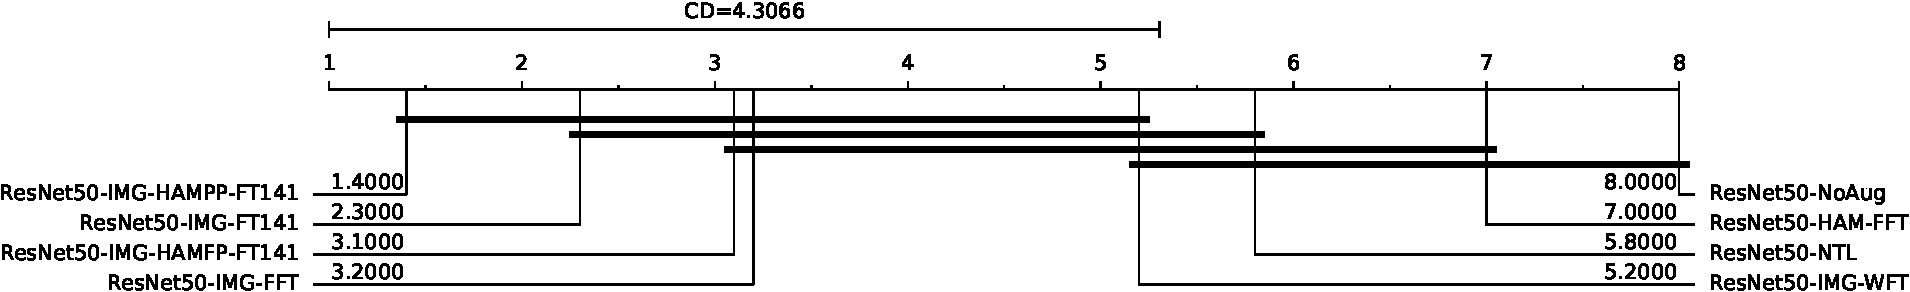
\includegraphics[width=\textwidth,keepaspectratio]{images/pretraining/CDRes-cropped.pdf}
	\caption[Accuracy critical difference diagram for ResNet50 based configurations]{Accuracy critical difference diagram for ResNet50 based configurations. The models are ordered by best to worst average ranking from left to right. The number beside a model’s name represents the average rank of the model. CD is the critical difference for Nemenyi post-hoc test. Thick horizontal line connects the models that are not statistically significantly different.}
	\label{fig:CD_ResNet}
\end{figure}

In the literature on recognizing EM from images, Čuk et al. \cite{Cuk2014} reported accuracies in the range of 69.23\% to 80.42\% using classical machine learning methods, and Burlina et al. \cite{Burlina2020} reported the best accuracy of 81.51\% using ResNet50 architecture for the case of EM vs all classification problems.
There was a common subset of images collected from the internet in both the dataset of Burlina et al. \cite{Burlina2018} and our Lyme dataset. ResNet50-Burlina model gave an accuracy of  76.05\% when tested on our full dataset as shown in Table \ref{tab:ResNet50-burlina-results}.
\begin{table}[tbh!]
	\centering
	\caption[Performance metrics of ResNet50-Burlina model trained by Burlina et al. \cite{Burlina2018} tested on the whole dataset of this study]{Performance metrics of ResNet50-Burlina model trained by Burlina et al. \cite{Burlina2018} tested on the whole dataset of this study. Within each cell, the value after $\pm$ symbol represents the standard deviation across five folds. Bold indicates the best result for each of the metrics.}
	\label{tab:ResNet50-burlina-results}
	\resizebox{\textwidth}{!}{%
		\begin{tabular}{llllllllllll}
			\toprule
			& \multicolumn{11}{c}{\textbf{Metric}}    \\ \cmidrule(l){2-12} 
			\multicolumn{1}{c}{\textbf{Model}} & \rotatebox{45}{Accuracy} & \rotatebox{45}{Sensitivity} & \rotatebox{45}{Specificity} & \rotatebox{45}{Precision} & \rotatebox{45}{NPV} & \rotatebox{45}{MCC} & \rotatebox{45}{Kappa} & \rotatebox{45}{LR$+$} & \rotatebox{45}{LR$-$} & \rotatebox{45}{F1-Score} & \rotatebox{45}{AUC}  \\ \midrule
			\begin{tabular}[c]{@{}l@{}}ResNet50-\\Burlina\end{tabular} & \begin{tabular}[c]{@{}l@{}}76.05\\ $\pm$0.74\end{tabular}& \begin{tabular}[c]{@{}l@{}}70.05\\ $\pm$3.6\end{tabular}& \begin{tabular}[c]{@{}l@{}}82.51\\ $\pm$3.31\end{tabular}& \begin{tabular}[c]{@{}l@{}}81.29\\ $\pm$2.1\end{tabular}& \begin{tabular}[c]{@{}l@{}}72.04\\ $\pm$1.71\end{tabular}& \begin{tabular}[c]{@{}l@{}}0.5294\\ $\pm$0.0132\end{tabular}& \begin{tabular}[c]{@{}l@{}}0.5229\\ $\pm$0.0145\end{tabular}& \begin{tabular}[c]{@{}l@{}}4.1017\\ $\pm$0.5172\end{tabular}& \begin{tabular}[c]{@{}l@{}}0.362\\ $\pm$0.0309\end{tabular}& \begin{tabular}[c]{@{}l@{}}0.7515\\ $\pm$0.0137\end{tabular}& \begin{tabular}[c]{@{}l@{}}0.481\\ $\pm$0.0509\end{tabular} \\ 
			\bottomrule
		\end{tabular}%
	}
\end{table} 
Performance metrics for the best performing configuration of all the CNN architectures used in this study are shown in Table \ref{tab:CNN-results}. ResNet50-141 achieved the best accuracy of 84.42\%. Most of the models except MobileNetV2-62, MobileNetV3Small-182, and NASNetMobile-617 showed good AUC values of above 90\% and good sensitivity suggesting that these CNNs can be a good choice for building pre-scanners for Lyme disease. Figure \ref{fig:CD_SOTA} shows the CD diagram in terms of accuracy for these models. The Friedman test null hypothesis was rejected with a $p$ value of 0.09564. From the CD diagram, we can see that ResNet50- 141 achieved the best average ranking followed by VGG19-13 and DenseNet121-379 respectively. Xception and Inception-based architectures had a similar ranking. NasNetMobile-617 ranked worst among all the models. The accuracy of the models varied from 81.3\% to 84.42\% and there is no statistically significant difference in terms of accuracy metric among most of the trained models. Overall, ResNet50-141 performed better in terms of various metrics (5 out of 11) as highlighted in Table \ref{tab:CNN-results}. We kept the confusion matrix, ROC curve, and cross-validation fold-wise details of all the trained models in Appendix Section \ref{sec:app-supply-pretrain} to make the chapter concise and readable.
\begin{figure}[]
	\centering
	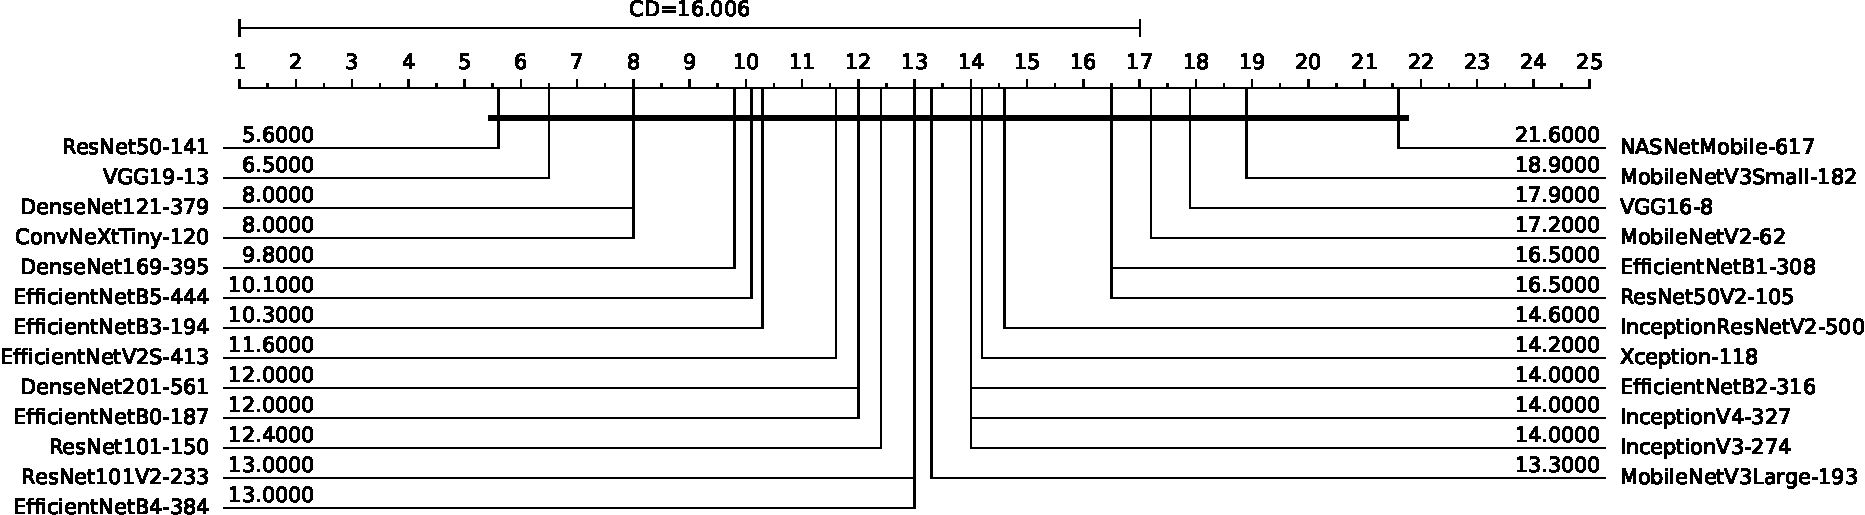
\includegraphics[width=\textwidth,keepaspectratio]{images/pretraining/CDAllSOTA-cropped.pdf}
	\caption[Accuracy critical difference diagram for the best performing configurations of the trained CNN models]{Accuracy critical difference diagram for the best performing configurations of the trained CNN models. The models are ordered by best to worst average ranking from left to right. The number beside a model’s name represents the average rank of the model. CD is the critical difference for Nemenyi post-hoc test. Thick horizontal line connects the models that are not statistically significantly different.}
	\label{fig:CD_SOTA}
\end{figure}

Table \ref{tab:complexity-table} summarizes the complexities of the CNN models used in this study.  The most lightweight model with the lowest number of parameters, FLOPs, and memory usage was MobileNetV3Small-182. InceptionResNetV2-500 has the highest number of parameters and memory usage and slowest inference time. Xception-118 was the fastest in terms of inference time. VGG19-13 required the highest number of FLOPs. ResNet50V2-105 required the least amount of time to train on average whereas, EfficientNetB5-444 was the slowest to train.

Table \ref{tab:gradcam} shows the Grad-CAM visualizations of the models trained on the same training fold for two test images. From the table, it can be seen that different versions of EfficientNet focused more on the lesion part of the image compared to other models. The squeeze-and-excitation \cite{Hu2020} channel attention used in EfficientNet can be the reason behind this behavior.

The experimental results showed that our proposed pre-training strategy utilizing dermoscopic dataset HAM10000 improved the performance of ImageNet pre-trained CNNs for recognizing clinical EM images. The results make it evident that CNNs have great potential to be used for Lyme disease pre-scanner application. Figure \ref{fig:bubble_chart} shows a bubble chart reporting model accuracy vs FLOPs. The size of each bubble represents the number of parameters of the model. This figure serves as a guideline for selecting models based on complexity and accuracy. It can be seen from the figure that EfficientNetB0-187 is a good choice with reasonable accuracy for resource-constrained mobile platforms. EfficientNetB0-187 also showed good results in Grad-CAM visualization. If resource constraint is not a problem, then RestNet50-141 can be used for the best accuracy.
\begin{figure}[h!]
	\centering
	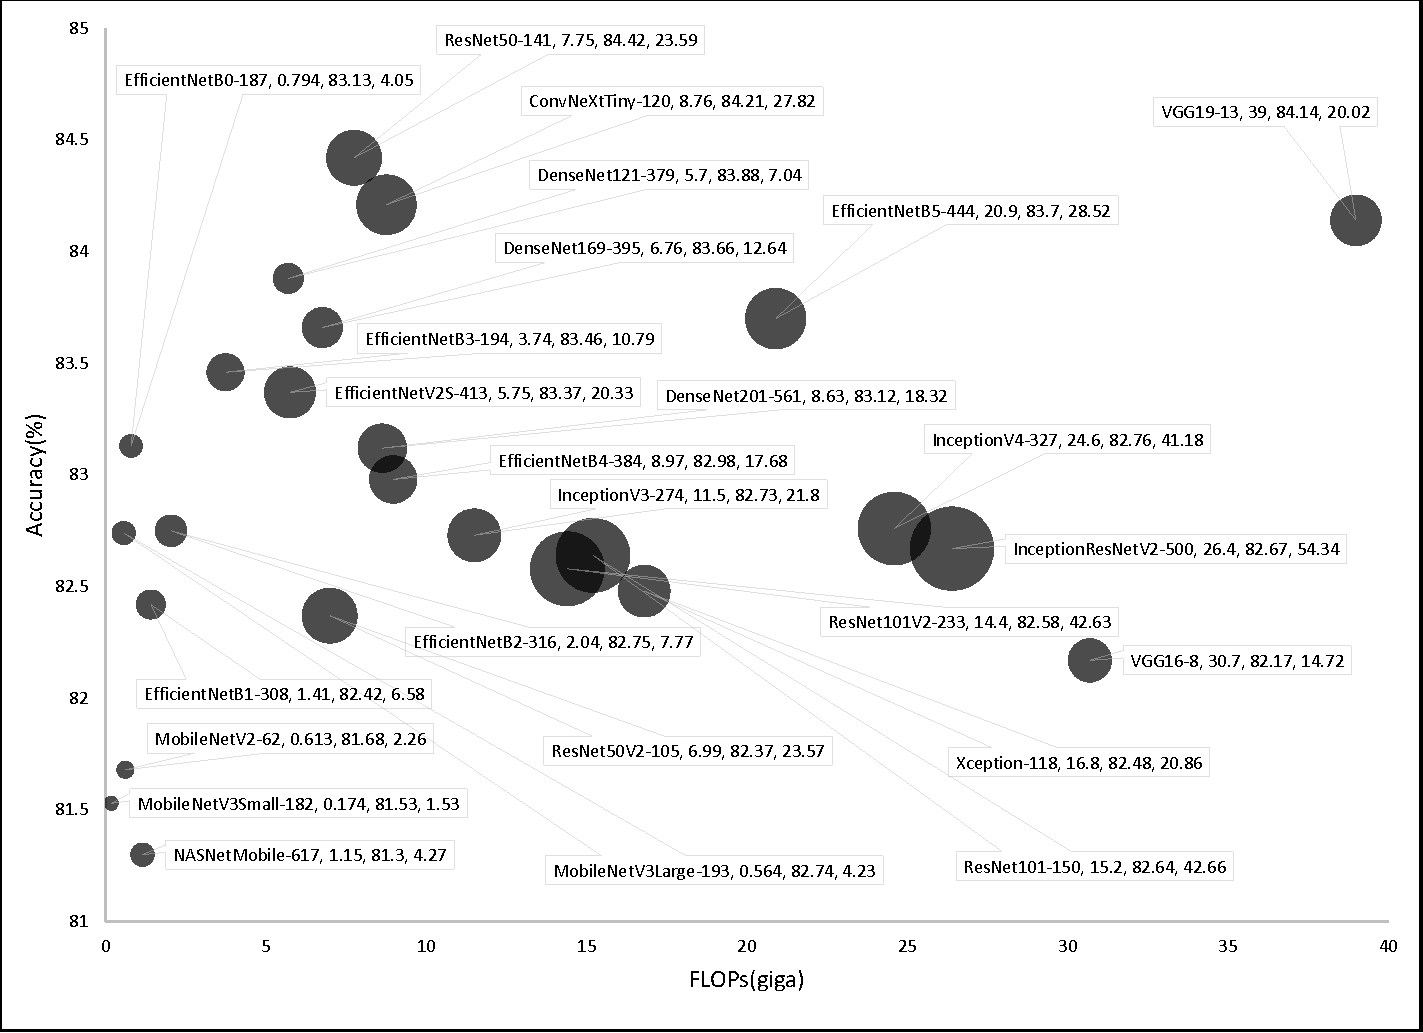
\includegraphics[width=\textwidth,keepaspectratio]{images/pretraining/bubble-chart-cropped.pdf}
	\caption[Bubble chart reporting model accuracy vs floating-point operations]{Bubble chart reporting model accuracy vs floating-point operations (FLOPs). The size of each bubble represents the number of model parameters measured in millions unit. Beside each model name the three values represent FLOPs, accuracy, and model parameters, respectively.}
	\label{fig:bubble_chart}
\end{figure}

Even the lightweight EfficientNetB0-187 model showed good performance, and it can be directly deployed in mobile devices without requiring an internet connection for processing the lesion image in a remote server. It can help people living in remote areas without good internet facilities with an initial assessment of the probability of Lyme disease. 

For this study, we utilized images from the internet alongside images collected from several hospitals in France. This approach was inspired by related studies on skin lesion analysis. 

Although a portion of images in our dataset was collected from the internet the annotation of the dataset is reliable because we ignored the online labels, and all the images were reannotated by expert dermatologists and infectiologists.

We made all the trained models publicly available, which can be utilized by others for transfer learning and building pre-scanners for Lyme disease. The trained CNN models are available at the link stated in Appendix Section \ref{sec:app-online-pretrain}.

%%%%%%%%%%%%%%%%%%%%%%%%%%%%%%%%%%%%%%%%%%%%%%%%%%%%%%%%%%%%%%%%%%%%%%%%
\section{Conclusion}\label{sec:concluion_pretrain}
%%%%%%%%%%%%%%%%%%%%%%%%%%%%%%%%%%%%%%%%%%%%%%%%%%%%%%%%%%%%%%%%%%%%%%%%
In this chapter, a pre-training strategy for improving clinical skin lesion image classification performance of ImageNet pre-trained convolutional neural networks by utilizing additional pre-training with dermoscopic images was proposed. We applied the strategy to benchmark twenty-five well-known CNNs based on predictive performance, complexity, significance tests, and heatmap visualization using a novel Lyme disease dataset to find out the effectiveness of CNNs for Lyme disease diagnosis from EM images. We also provided guidelines for model selection. We found that even the lightweight models like EffiicentNetB0 performed well suggesting the application of CNNs for Lyme disease pre-scanner mobile applications which can help people with an initial assessment of the probability of Lyme disease and referring them to expert dermatologist for further diagnosis. Resource intensive models like ResNet50 can be effective for building computer applications to assist non-expert practitioners with identifying EM.


\begin{tcolorbox}[enhanced,attach boxed title to top center={yshift=-3mm,yshifttext=-1mm},
	coltitle=black, colback=blue!5!white,colframe=blue!75!black,colbacktitle=violet!50!white,
	title=Key Points (Chapter \ref{chap:Pretraining}),fonttitle=\bfseries,
	boxed title style={colframe=black} ]
	\begin{itemize}
		\item We proposed a pre-training strategy of fine-tuning some layers from the end of an ImageNet pre-trained CNN architecture using a dermoscopic dataset before training the model on a clinical skin lesion dataset.
		\item The proposed pre-training strategy seemed effective for increasing model performance based on experimentation using a novel Lyme disease dataset.
		\item We benchmarked several state-of-the-art CNN architectures on the novel Lyme dataset utilizing our pre-training strategy.
		\item Experimental results suggest that even lightweight CNNs can be effective for Lyme disease pre-scanner mobile applications.
	\end{itemize}
\end{tcolorbox}

%%%%%%%%%%%%%Complexity Table%%%%%%%%%%%%%%%
\begin{table}[h!]
	\centering
	\caption[Complexity metrics of trained CNN models]{Complexity metrics of trained CNN models. Bold indicates the best result for each of the metrics.}
	\label{tab:complexity-table}
	\resizebox{\textwidth}{!}{%
		\begin{tabular}{@{}lccccc@{}}
			\toprule
			\multicolumn{1}{c}{\textbf{Model}} &
			\multicolumn{1}{c}{\textbf{Parameters}} &
			\multicolumn{1}{c}{\textbf{FLOPs}} &
			\multicolumn{1}{c}{\textbf{Average training time}} &
			\multicolumn{1}{c}{\textbf{GPU usage}} &
			\multicolumn{1}{c}{\textbf{Average inference time}} \\
			&
			\multicolumn{1}{c}{(million)} &
			\multicolumn{1}{c}{(giga)} &
			\multicolumn{1}{c}{(sec per epoch)} &
			\multicolumn{1}{c}{(megabyte)} &
			\multicolumn{1}{c}{(sec per image)} \\ \midrule
			VGG16-8               & 14.72         & 30.7           & 111         & 565          & 0.0426 \\
			VGG19-13              & 20.02         & 39             & 164         & 565          & 0.0431 \\
			ResNet50-141          & 23.59         & 7.75           & 113         & 821          & 0.0484 \\
			ResNet101-150         & 42.66         & 15.2           & 123.33      & 821          & 0.0539 \\
			ResNet50V2-105        & 23.57         & 6.99           & 76          & 821          & 0.0464 \\
			ResNet101V2-233       & 42.63         & 14.4           & 152         & 821          & 0.0599 \\
			InceptionV3-274       & 21.8          & 11.5           & 133         & 821          & 0.054  \\
			InceptionV4-327       & 41.18         & 24.6           & 223.33      & 1333         & 0.0735 \\
			InceptionResNetV2-500 & 54.34         & 26.4           & 281.33      & 1333         & 0.0958 \\
			Xception-118          & 20.86         & 16.8           & 243.33      & 821          & 0.0392 \\
			DenseNet121-379       & 7.04          & 5.7            & 140.67      & 437          & 0.0673 \\
			DenseNet169-395       & 12.64         & 6.76           & 130         & 565          & 0.0686 \\
			DenseNet201-561       & 18.32         & 8.63           & 182.67      & 565          & 0.084  \\
			MobileNetV2-62        & 2.26          & 0.613          & 78          & \textbf{341} & 0.0429 \\
			MobileNetV3Small-182  & \textbf{1.53} & \textbf{0.174} & 81          & \textbf{341} & 0.0444 \\
			MobileNetV3Large-193  & 4.23          & 0.564          & 86.33       & 373          & 0.0444 \\
			NASNetMobile -617     & 4.27          & 1.15           & 152         & 373          & 0.0741 \\
			EfficientNetB0-187    & 4.05          & 0.794          & 87          & 373          & 0.0523 \\
			EfficientNetB1-308    & 6.58          & 1.41           & 158.33      & 437          & 0.0546 \\
			EfficientNetB2-316    & 7.77          & 2.04           & 210         & 437          & 0.0565 \\
			EfficientNetB3-194    & 10.79         & 3.74           & 143         & 565          & 0.0648 \\
			EfficientNetB4-384    & 17.68         & 8.97           & 431         & 565          & 0.0614 \\
			EfficientNetB5-444    & 28.52         & 20.9           & 771         & 821          & 0.0659 \\
			EfficientNetV2S-413   & 20.33         & 5.75           & \textbf{50} & 591          & 0.934  \\
			ConvNeXtTiny-120      & 27.82         & 8.76           & 95          & 847          & 0.0664 \\ \bottomrule
		\end{tabular}%
	}
\end{table}
%%%%%%%%%%%%%Complexity Table%%%%%%%%%%%%%%%

%%%%%%%%%%%%%BIG TABLE%%%%%%%%%%%%%%%%%%%
\begin{table}[]
	\centering
	\caption[Five-fold cross-validation performance metrics for the best performing configurations of the trained CNN models]{Five-fold cross-validation performance metrics for the best performing configurations of the trained CNN models. Within each cell, the value after (±) symbol represents the standard deviation across five folds. Bold indicates the best result for each of the metrics.}
	\label{tab:CNN-results}
	\resizebox{\textwidth}{!}{%
		\begin{tabular}{llllllllllll}
			\toprule
			& \multicolumn{11}{c}{\textbf{Metric}}    \\ \cmidrule(l){2-12} 
			\multicolumn{1}{c}{\textbf{Model}} & \rotatebox{45}{Accuracy} & \rotatebox{45}{Sensitivity} & \rotatebox{45}{Specificity} & \rotatebox{45}{Precision} & \rotatebox{45}{NPV} & \rotatebox{45}{MCC} & \rotatebox{45}{Kappa} & \rotatebox{45}{LR$+$} & \rotatebox{45}{LR$-$} & \rotatebox{45}{F1-Score} & \rotatebox{45}{AUC}  \\ \midrule
			VGG16-8 & \begin{tabular}[c]{@{}l@{}}82.17 \\ $\pm$ 1.23\end{tabular}& \begin{tabular}[c]{@{}l@{}}85.77 \\ $\pm$ 3.58\end{tabular}& \begin{tabular}[c]{@{}l@{}}78.31 \\ $\pm$ 4.36\end{tabular}& \begin{tabular}[c]{@{}l@{}}81.12 \\ $\pm$ 2.62\end{tabular}& \begin{tabular}[c]{@{}l@{}}83.88 \\ $\pm$ 3.02\end{tabular}& \begin{tabular}[c]{@{}l@{}}0.6453 \\ $\pm$ 0.0253\end{tabular}& \begin{tabular}[c]{@{}l@{}}0.6422 \\ $\pm$ 0.0249\end{tabular}& \begin{tabular}[c]{@{}l@{}}4.0983 \\ $\pm$ 0.7329\end{tabular}& \begin{tabular}[c]{@{}l@{}}0.1802 \\ $\pm$ 0.0388\end{tabular}& \begin{tabular}[c]{@{}l@{}}0.8328 \\ $\pm$ 0.0116\end{tabular}& \begin{tabular}[c]{@{}l@{}}0.9011 \\ $\pm$ 0.0079\end{tabular}\\
			\cmidrule(lr){1-12}
			
			VGG19-13 & \begin{tabular}[c]{@{}l@{}}84.14 \\ $\pm$ 1.62\end{tabular}& \begin{tabular}[c]{@{}l@{}}85.29 \\ $\pm$ 1.69\end{tabular}& \begin{tabular}[c]{@{}l@{}}82.9 \\ $\pm$ 2.63\end{tabular}& \begin{tabular}[c]{@{}l@{}}\textbf{84.32} \\ $\pm$ 1.97\end{tabular}& \begin{tabular}[c]{@{}l@{}}84.0 \\ $\pm$ 1.67\end{tabular}& \begin{tabular}[c]{@{}l@{}}0.6826 \\ $\pm$ 0.0323\end{tabular}& \begin{tabular}[c]{@{}l@{}}0.6823 \\ $\pm$ 0.0326\end{tabular}& \begin{tabular}[c]{@{}l@{}}5.0924 \\ $\pm$ 0.6884\end{tabular}& \begin{tabular}[c]{@{}l@{}}0.1777 \\ $\pm$ 0.0214\end{tabular}& \begin{tabular}[c]{@{}l@{}}0.8479 \\ $\pm$ 0.0146\end{tabular}& \begin{tabular}[c]{@{}l@{}}0.913 \\ $\pm$ 0.0074\end{tabular}\\ 
			\cmidrule(lr){1-12}
			
			ResNet50-141 & \begin{tabular}[c]{@{}l@{}}\textbf{84.42} \\ $\pm$ 1.36\end{tabular}& \begin{tabular}[c]{@{}l@{}}87.93 \\ $\pm$ 1.47\end{tabular}& \begin{tabular}[c]{@{}l@{}}80.65 \\ $\pm$ 3.59\end{tabular}& \begin{tabular}[c]{@{}l@{}}83.1 \\ $\pm$ 2.49\end{tabular}& \begin{tabular}[c]{@{}l@{}}86.19 \\ $\pm$ 1.27\end{tabular}& \begin{tabular}[c]{@{}l@{}}\textbf{0.6893} \\ $\pm$ 0.0263\end{tabular}& \begin{tabular}[c]{@{}l@{}}\textbf{0.6874} \\ $\pm$ 0.0277\end{tabular}& \begin{tabular}[c]{@{}l@{}}4.703 \\ $\pm$ 0.8624\end{tabular}& \begin{tabular}[c]{@{}l@{}}0.1493 \\ $\pm$ 0.0155\end{tabular}& \begin{tabular}[c]{@{}l@{}}\textbf{0.8541} \\ $\pm$ 0.0106\end{tabular}& \begin{tabular}[c]{@{}l@{}}\textbf{0.9189} \\ $\pm$ 0.0115\end{tabular}\\ 
			\cmidrule(lr){1-12}
			
			\begin{tabular}[c]{@{}l@{}}ResNet50V2-\\105\end{tabular} & \begin{tabular}[c]{@{}l@{}}82.37 \\ $\pm$ 2.15\end{tabular}& \begin{tabular}[c]{@{}l@{}}85.53 \\ $\pm$ 3.35\end{tabular}& \begin{tabular}[c]{@{}l@{}}78.96 \\ $\pm$ 6.13\end{tabular}& \begin{tabular}[c]{@{}l@{}}81.66 \\ $\pm$ 3.83\end{tabular}& \begin{tabular}[c]{@{}l@{}}83.72 \\ $\pm$ 2.63\end{tabular}& \begin{tabular}[c]{@{}l@{}}0.6493 \\ $\pm$ 0.0411\end{tabular}& \begin{tabular}[c]{@{}l@{}}0.6461 \\ $\pm$ 0.0439\end{tabular}& \begin{tabular}[c]{@{}l@{}}4.3618 \\ $\pm$ 1.0495\end{tabular}& \begin{tabular}[c]{@{}l@{}}0.1819 \\ $\pm$ 0.0349\end{tabular}& \begin{tabular}[c]{@{}l@{}}0.8343 \\ $\pm$ 0.017\end{tabular}& \begin{tabular}[c]{@{}l@{}}0.9013 \\ $\pm$ 0.0133\end{tabular}\\ 
			\cmidrule(lr){1-12}
			
			\begin{tabular}[c]{@{}l@{}}ResNet101V2-\\233\end{tabular} & \begin{tabular}[c]{@{}l@{}}82.58 \\ $\pm$ 2.21\end{tabular}& \begin{tabular}[c]{@{}l@{}}81.9 \\ $\pm$ 4.78\end{tabular}& \begin{tabular}[c]{@{}l@{}}\textbf{83.32} \\ $\pm$ 3.71\end{tabular}& \begin{tabular}[c]{@{}l@{}}84.17 \\ $\pm$ 2.55\end{tabular}& \begin{tabular}[c]{@{}l@{}}81.31 \\ $\pm$ 3.7\end{tabular}& \begin{tabular}[c]{@{}l@{}}0.6535 \\ $\pm$ 0.0429\end{tabular}& \begin{tabular}[c]{@{}l@{}}0.6515 \\ $\pm$ 0.0439\end{tabular}& \begin{tabular}[c]{@{}l@{}}\textbf{5.104} \\ $\pm$ 0.9811\end{tabular}& \begin{tabular}[c]{@{}l@{}}0.2163 \\ $\pm$ 0.0541\end{tabular}& \begin{tabular}[c]{@{}l@{}}0.8292 \\ $\pm$ 0.0254\end{tabular}& \begin{tabular}[c]{@{}l@{}}0.9118 \\ $\pm$ 0.0149\end{tabular}\\ 
			\cmidrule(lr){1-12}
			
			\begin{tabular}[c]{@{}l@{}}InceptionV3-\\274\end{tabular} & \begin{tabular}[c]{@{}l@{}}82.73 \\ $\pm$ 2.08\end{tabular}& \begin{tabular}[c]{@{}l@{}}86.57 \\ $\pm$ 2.42\end{tabular}& \begin{tabular}[c]{@{}l@{}}78.6 \\ $\pm$ 2.8\end{tabular}& \begin{tabular}[c]{@{}l@{}}81.33 \\ $\pm$ 2.12\end{tabular}& \begin{tabular}[c]{@{}l@{}}84.52 \\ $\pm$ 2.52\end{tabular}& \begin{tabular}[c]{@{}l@{}}0.6551 \\ $\pm$ 0.0419\end{tabular}& \begin{tabular}[c]{@{}l@{}}0.6533 \\ $\pm$ 0.0419\end{tabular}& \begin{tabular}[c]{@{}l@{}}4.1259 \\ $\pm$ 0.639\end{tabular}& \begin{tabular}[c]{@{}l@{}}0.1714 \\ $\pm$ 0.0328\end{tabular}& \begin{tabular}[c]{@{}l@{}}0.8385 \\ $\pm$ 0.0195\end{tabular}& \begin{tabular}[c]{@{}l@{}}0.9052 \\ $\pm$ 0.0185\end{tabular}\\ 
			
			\cmidrule(lr){1-12}
			
			\begin{tabular}[c]{@{}l@{}}InceptionV4-\\327\end{tabular} & \begin{tabular}[c]{@{}l@{}}82.76 \\ $\pm$ 1.78\end{tabular}& \begin{tabular}[c]{@{}l@{}}85.7 \\ $\pm$ 3.96\end{tabular}& \begin{tabular}[c]{@{}l@{}}79.58 \\ $\pm$ 2.87\end{tabular}& \begin{tabular}[c]{@{}l@{}}81.92 \\ $\pm$ 1.8\end{tabular}& \begin{tabular}[c]{@{}l@{}}84.02 \\ $\pm$ 3.41\end{tabular}& \begin{tabular}[c]{@{}l@{}}0.6561 \\ $\pm$ 0.0358\end{tabular}& \begin{tabular}[c]{@{}l@{}}0.6541 \\ $\pm$ 0.0353\end{tabular}& \begin{tabular}[c]{@{}l@{}}4.2716 \\ $\pm$ 0.5734\end{tabular}& \begin{tabular}[c]{@{}l@{}}0.179 \\ $\pm$ 0.0465\end{tabular}& \begin{tabular}[c]{@{}l@{}}0.837 \\ $\pm$ 0.0197\end{tabular}& \begin{tabular}[c]{@{}l@{}}0.9092 \\ $\pm$ 0.019\end{tabular}\\ 
			
			\cmidrule(lr){1-12}
			
			\begin{tabular}[c]{@{}l@{}}Inception\\ResNetV2-500\end{tabular} & \begin{tabular}[c]{@{}l@{}}82.67\\ $\pm$2.06\end{tabular}& \begin{tabular}[c]{@{}l@{}}83.54\\ $\pm$3.88\end{tabular}& \begin{tabular}[c]{@{}l@{}}81.74\\ $\pm$3.16\end{tabular}& \begin{tabular}[c]{@{}l@{}}83.17\\ $\pm$2.16\end{tabular}& \begin{tabular}[c]{@{}l@{}}82.37\\ $\pm$3.32\end{tabular}& \begin{tabular}[c]{@{}l@{}}0.6541\\ $\pm$0.0406\end{tabular}& \begin{tabular}[c]{@{}l@{}}0.653\\ $\pm$0.041\end{tabular}& \begin{tabular}[c]{@{}l@{}}4.6886\\ $\pm$0.7264\end{tabular}& \begin{tabular}[c]{@{}l@{}}0.2009\\ $\pm$0.0456\end{tabular}& \begin{tabular}[c]{@{}l@{}}0.8329\\ $\pm$0.0218\end{tabular}& \begin{tabular}[c]{@{}l@{}}0.9011\\ $\pm$0.0133\end{tabular}\\ 
			
			\cmidrule(lr){1-12}
			
			Xception-118 & \begin{tabular}[c]{@{}l@{}}82.48\\ $\pm$2.45\end{tabular}& \begin{tabular}[c]{@{}l@{}}83.16\\ $\pm$5.1\end{tabular}& \begin{tabular}[c]{@{}l@{}}81.75\\ $\pm$2.76\end{tabular}& \begin{tabular}[c]{@{}l@{}}83.08\\ $\pm$1.94\end{tabular}& \begin{tabular}[c]{@{}l@{}}82.16\\ $\pm$4.4\end{tabular}& \begin{tabular}[c]{@{}l@{}}0.6507\\ $\pm$0.0487\end{tabular}& \begin{tabular}[c]{@{}l@{}}0.6492\\ $\pm$0.0484\end{tabular}& \begin{tabular}[c]{@{}l@{}}4.6434\\ $\pm$0.6571\end{tabular}& \begin{tabular}[c]{@{}l@{}}0.2054\\ $\pm$0.0609\end{tabular}& \begin{tabular}[c]{@{}l@{}}0.8304\\ $\pm$0.0276\end{tabular}& \begin{tabular}[c]{@{}l@{}}0.9081\\ $\pm$0.0148\end{tabular}\\ 
			
			\cmidrule(lr){1-12}
			
			\begin{tabular}[c]{@{}l@{}}DenseNet121-\\379\end{tabular} & \begin{tabular}[c]{@{}l@{}}83.88\\ $\pm$0.92\end{tabular}& \begin{tabular}[c]{@{}l@{}}85.85\\ $\pm$1.76\end{tabular}& \begin{tabular}[c]{@{}l@{}}81.75\\ $\pm$0.95\end{tabular}& \begin{tabular}[c]{@{}l@{}}83.49\\ $\pm$0.69\end{tabular}& \begin{tabular}[c]{@{}l@{}}84.35\\ $\pm$1.57\end{tabular}& \begin{tabular}[c]{@{}l@{}}0.6773\\ $\pm$0.0186\end{tabular}& \begin{tabular}[c]{@{}l@{}}0.6768\\ $\pm$0.0184\end{tabular}& \begin{tabular}[c]{@{}l@{}}4.7169\\ $\pm$0.254\end{tabular}& \begin{tabular}[c]{@{}l@{}}0.173\\ $\pm$0.0211\end{tabular}& \begin{tabular}[c]{@{}l@{}}0.8465\\ $\pm$0.01\end{tabular}& \begin{tabular}[c]{@{}l@{}}0.9158\\ $\pm$0.0097\end{tabular}\\ 
			
			\cmidrule(lr){1-12}
			
			\begin{tabular}[c]{@{}l@{}}DenseNet169-\\395\end{tabular} & \begin{tabular}[c]{@{}l@{}}83.66\\ $\pm$1.25\end{tabular}& \begin{tabular}[c]{@{}l@{}}\textbf{88.6}\\ $\pm$3.59\end{tabular}& \begin{tabular}[c]{@{}l@{}}78.35\\ $\pm$2.75\end{tabular}& \begin{tabular}[c]{@{}l@{}}81.54\\ $\pm$1.53\end{tabular}& \begin{tabular}[c]{@{}l@{}}\textbf{86.68}\\ $\pm$3.33\end{tabular}& \begin{tabular}[c]{@{}l@{}}0.6758\\ $\pm$0.0265\end{tabular}& \begin{tabular}[c]{@{}l@{}}0.6717\\ $\pm$0.0249\end{tabular}& \begin{tabular}[c]{@{}l@{}}4.1454\\ $\pm$0.4187\end{tabular}& \begin{tabular}[c]{@{}l@{}}\textbf{0.1446}\\ $\pm$0.0414\end{tabular}& \begin{tabular}[c]{@{}l@{}}0.8486\\ $\pm$0.0138\end{tabular}& \begin{tabular}[c]{@{}l@{}}0.9123\\ $\pm$0.0129\end{tabular}\\ 
			
			\cmidrule(lr){1-12}
			
			\begin{tabular}[c]{@{}l@{}}DenseNet201-\\561\end{tabular} & \begin{tabular}[c]{@{}l@{}}83.12\\ $\pm$1.11\end{tabular}& \begin{tabular}[c]{@{}l@{}}85.61\\ $\pm$1.81\end{tabular}& \begin{tabular}[c]{@{}l@{}}80.45\\ $\pm$3.92\end{tabular}& \begin{tabular}[c]{@{}l@{}}82.61\\ $\pm$2.7\end{tabular}& \begin{tabular}[c]{@{}l@{}}83.93\\ $\pm$1.13\end{tabular}& \begin{tabular}[c]{@{}l@{}}0.663\\ $\pm$0.0221\end{tabular}& \begin{tabular}[c]{@{}l@{}}0.6615\\ $\pm$0.0228\end{tabular}& \begin{tabular}[c]{@{}l@{}}4.5729\\ $\pm$0.9885\end{tabular}& \begin{tabular}[c]{@{}l@{}}0.1783\\ $\pm$0.0153\end{tabular}& \begin{tabular}[c]{@{}l@{}}0.8403\\ $\pm$0.0073\end{tabular}& \begin{tabular}[c]{@{}l@{}}0.9125\\ $\pm$0.0083\end{tabular}\\ 
			
			\cmidrule(lr){1-12}
			
			
			\begin{tabular}[c]{@{}l@{}}MobileNetV2-\\62\end{tabular} & \begin{tabular}[c]{@{}l@{}}81.68\\ $\pm$1.99\end{tabular}& \begin{tabular}[c]{@{}l@{}}81.94\\ $\pm$3.49\end{tabular}& \begin{tabular}[c]{@{}l@{}}81.39\\ $\pm$1.26\end{tabular}& \begin{tabular}[c]{@{}l@{}}82.55\\ $\pm$1.21\end{tabular}& \begin{tabular}[c]{@{}l@{}}80.85\\ $\pm$3.09\end{tabular}& \begin{tabular}[c]{@{}l@{}}0.6337\\ $\pm$0.0394\end{tabular}& \begin{tabular}[c]{@{}l@{}}0.6332\\ $\pm$0.0395\end{tabular}& \begin{tabular}[c]{@{}l@{}}4.4256\\ $\pm$0.3596\end{tabular}& \begin{tabular}[c]{@{}l@{}}0.222\\ $\pm$0.0441\end{tabular}& \begin{tabular}[c]{@{}l@{}}0.8222\\ $\pm$0.0218\end{tabular}& \begin{tabular}[c]{@{}l@{}}0.8933\\ $\pm$0.0135\end{tabular}\\ 
			
			\cmidrule(lr){1-12}
			
			\begin{tabular}[c]{@{}l@{}}MobileNetV3\\Small-182\end{tabular} & \begin{tabular}[c]{@{}l@{}}81.53\\ $\pm$1.98\end{tabular}& \begin{tabular}[c]{@{}l@{}}84.93\\ $\pm$3.29\end{tabular}& \begin{tabular}[c]{@{}l@{}}77.87\\ $\pm$3.89\end{tabular}& \begin{tabular}[c]{@{}l@{}}80.6\\ $\pm$2.55\end{tabular}& \begin{tabular}[c]{@{}l@{}}82.91\\ $\pm$2.85\end{tabular}& \begin{tabular}[c]{@{}l@{}}0.6315\\ $\pm$0.0398\end{tabular}& \begin{tabular}[c]{@{}l@{}}0.6294\\ $\pm$0.04\end{tabular}& \begin{tabular}[c]{@{}l@{}}3.9496\\ $\pm$0.6356\end{tabular}& \begin{tabular}[c]{@{}l@{}}0.1933\\ $\pm$0.0386\end{tabular}& \begin{tabular}[c]{@{}l@{}}0.8265\\ $\pm$0.0186\end{tabular}& \begin{tabular}[c]{@{}l@{}}0.896\\ $\pm$0.013\end{tabular}\\ 
			
			\cmidrule(lr){1-12}
			
			\begin{tabular}[c]{@{}l@{}}MobileNetV3\\Large-193\end{tabular} & \begin{tabular}[c]{@{}l@{}}82.74\\ $\pm$2.17\end{tabular}& \begin{tabular}[c]{@{}l@{}}83.69\\ $\pm$0.43\end{tabular}& \begin{tabular}[c]{@{}l@{}}81.71\\ $\pm$4.6\end{tabular}& \begin{tabular}[c]{@{}l@{}}83.26\\ $\pm$3.39\end{tabular}& \begin{tabular}[c]{@{}l@{}}82.3\\ $\pm$0.89\end{tabular}& \begin{tabular}[c]{@{}l@{}}0.6548\\ $\pm$0.0437\end{tabular}& \begin{tabular}[c]{@{}l@{}}0.6542\\ $\pm$0.0442\end{tabular}& \begin{tabular}[c]{@{}l@{}}4.8573\\ $\pm$1.1585\end{tabular}& \begin{tabular}[c]{@{}l@{}}0.2002\\ $\pm$0.0117\end{tabular}& \begin{tabular}[c]{@{}l@{}}0.8344\\ $\pm$0.017\end{tabular}& \begin{tabular}[c]{@{}l@{}}0.9034\\ $\pm$0.0094\end{tabular}\\ 
			
			\cmidrule(lr){1-12}
			
			\begin{tabular}[c]{@{}l@{}}NASNet\\Mobile-617\end{tabular} & \begin{tabular}[c]{@{}l@{}}81.3\\ $\pm$1.45\end{tabular}& \begin{tabular}[c]{@{}l@{}}83.2\\ $\pm$1.66\end{tabular}& \begin{tabular}[c]{@{}l@{}}79.25\\ $\pm$3.98\end{tabular}& \begin{tabular}[c]{@{}l@{}}81.29\\ $\pm$2.65\end{tabular}& \begin{tabular}[c]{@{}l@{}}81.48\\ $\pm$1.07\end{tabular}& \begin{tabular}[c]{@{}l@{}}0.6261\\ $\pm$0.0287\end{tabular}& \begin{tabular}[c]{@{}l@{}}0.6251\\ $\pm$0.0297\end{tabular}& \begin{tabular}[c]{@{}l@{}}4.1452\\ $\pm$0.7283\end{tabular}& \begin{tabular}[c]{@{}l@{}}0.2117\\ $\pm$0.0156\end{tabular}& \begin{tabular}[c]{@{}l@{}}0.8219\\ $\pm$0.0108\end{tabular}& \begin{tabular}[c]{@{}l@{}}0.8897\\ $\pm$0.0152\end{tabular}\\ 
			
			
			\cmidrule(lr){1-12}
			
			\begin{tabular}[c]{@{}l@{}}EfficientNet\\B0-187\end{tabular} & \begin{tabular}[c]{@{}l@{}}83.13\\ $\pm$1.2\end{tabular}& \begin{tabular}[c]{@{}l@{}}85.21\\ $\pm$3.91\end{tabular}& \begin{tabular}[c]{@{}l@{}}80.89\\ $\pm$2.95\end{tabular}& \begin{tabular}[c]{@{}l@{}}82.83\\ $\pm$1.75\end{tabular}& \begin{tabular}[c]{@{}l@{}}83.79\\ $\pm$3.19\end{tabular}& \begin{tabular}[c]{@{}l@{}}0.6636\\ $\pm$0.0244\end{tabular}& \begin{tabular}[c]{@{}l@{}}0.6618\\ $\pm$0.0237\end{tabular}& \begin{tabular}[c]{@{}l@{}}4.5522\\ $\pm$0.6116\end{tabular}& \begin{tabular}[c]{@{}l@{}}0.1817\\ $\pm$0.0427\end{tabular}& \begin{tabular}[c]{@{}l@{}}0.8392\\ $\pm$0.0147\end{tabular}& \begin{tabular}[c]{@{}l@{}}0.9094\\ $\pm$0.0129\end{tabular}\\ 
			
			\cmidrule(lr){1-12}
			
			\begin{tabular}[c]{@{}l@{}}EfficientNet\\B1-308\end{tabular} & \begin{tabular}[c]{@{}l@{}}82.42\\ $\pm$1.04\end{tabular}& \begin{tabular}[c]{@{}l@{}}85.85\\ $\pm$2.14\end{tabular}& \begin{tabular}[c]{@{}l@{}}78.71\\ $\pm$3.75\end{tabular}& \begin{tabular}[c]{@{}l@{}}81.37\\ $\pm$2.34\end{tabular}& \begin{tabular}[c]{@{}l@{}}83.9\\ $\pm$1.59\end{tabular}& \begin{tabular}[c]{@{}l@{}}0.6492\\ $\pm$0.0202\end{tabular}& \begin{tabular}[c]{@{}l@{}}0.647\\ $\pm$0.0214\end{tabular}& \begin{tabular}[c]{@{}l@{}}4.1494\\ $\pm$0.6707\end{tabular}& \begin{tabular}[c]{@{}l@{}}0.179\\ $\pm$0.0209\end{tabular}& \begin{tabular}[c]{@{}l@{}}0.835\\ $\pm$0.0074\end{tabular}& \begin{tabular}[c]{@{}l@{}}0.9088\\ $\pm$0.0134\end{tabular}\\ 
			
			
			\cmidrule(lr){1-12}
			
			\begin{tabular}[c]{@{}l@{}}EfficientNet\\B2-316\end{tabular} & \begin{tabular}[c]{@{}l@{}}82.75\\ $\pm$1.4\end{tabular}& \begin{tabular}[c]{@{}l@{}}84.95\\ $\pm$3.41\end{tabular}& \begin{tabular}[c]{@{}l@{}}80.39\\ $\pm$3.02\end{tabular}& \begin{tabular}[c]{@{}l@{}}82.39\\ $\pm$1.91\end{tabular}& \begin{tabular}[c]{@{}l@{}}83.4\\ $\pm$2.69\end{tabular}& \begin{tabular}[c]{@{}l@{}}0.6556\\ $\pm$0.0276\end{tabular}& \begin{tabular}[c]{@{}l@{}}0.6542\\ $\pm$0.0279\end{tabular}& \begin{tabular}[c]{@{}l@{}}4.4211\\ $\pm$0.6202\end{tabular}& \begin{tabular}[c]{@{}l@{}}0.1865\\ $\pm$0.0379\end{tabular}& \begin{tabular}[c]{@{}l@{}}0.8359\\ $\pm$0.0158\end{tabular}& \begin{tabular}[c]{@{}l@{}}0.9075\\ $\pm$0.0082\end{tabular}\\ 
			
			\cmidrule(lr){1-12}
			
			\begin{tabular}[c]{@{}l@{}}EfficientNet\\B3-194\end{tabular} & \begin{tabular}[c]{@{}l@{}}83.46\\ $\pm$0.87\end{tabular}& \begin{tabular}[c]{@{}l@{}}85.15\\ $\pm$4.28\end{tabular}& \begin{tabular}[c]{@{}l@{}}81.64\\ $\pm$2.9\end{tabular}& \begin{tabular}[c]{@{}l@{}}83.4\\ $\pm$1.6\end{tabular}& \begin{tabular}[c]{@{}l@{}}83.9\\ $\pm$3.14\end{tabular}& \begin{tabular}[c]{@{}l@{}}0.6704\\ $\pm$0.0157\end{tabular}& \begin{tabular}[c]{@{}l@{}}0.6685\\ $\pm$0.0167\end{tabular}& \begin{tabular}[c]{@{}l@{}}4.7361\\ $\pm$0.6283\end{tabular}& \begin{tabular}[c]{@{}l@{}}0.1803\\ $\pm$0.0443\end{tabular}& \begin{tabular}[c]{@{}l@{}}0.8416\\ $\pm$0.0144\end{tabular}& \begin{tabular}[c]{@{}l@{}}0.9163\\ $\pm$0.0074\end{tabular}\\ 
			
			\cmidrule(lr){1-12}
			
			\begin{tabular}[c]{@{}l@{}}EfficientNet\\B4-384\end{tabular} & \begin{tabular}[c]{@{}l@{}}82.98\\ $\pm$1.31\end{tabular}& \begin{tabular}[c]{@{}l@{}}87.55\\ $\pm$2.2\end{tabular}& \begin{tabular}[c]{@{}l@{}}78.06\\ $\pm$3.76\end{tabular}& \begin{tabular}[c]{@{}l@{}}81.2\\ $\pm$2.33\end{tabular}& \begin{tabular}[c]{@{}l@{}}85.46\\ $\pm$1.76\end{tabular}& \begin{tabular}[c]{@{}l@{}}0.6613\\ $\pm$0.0249\end{tabular}& \begin{tabular}[c]{@{}l@{}}0.6581\\ $\pm$0.0268\end{tabular}& \begin{tabular}[c]{@{}l@{}}4.0946\\ $\pm$0.6159\end{tabular}& \begin{tabular}[c]{@{}l@{}}0.1589\\ $\pm$0.0233\end{tabular}& \begin{tabular}[c]{@{}l@{}}0.842\\ $\pm$0.0107\end{tabular}& \begin{tabular}[c]{@{}l@{}}0.9138\\ $\pm$0.0074\end{tabular}\\ 
			
			\cmidrule(lr){1-12}
			
			\begin{tabular}[c]{@{}l@{}}EfficientNet\\B5-444\end{tabular} & \begin{tabular}[c]{@{}l@{}}83.7\\ $\pm$1.21\end{tabular}& \begin{tabular}[c]{@{}l@{}}86.85\\ $\pm$2.89\end{tabular}& \begin{tabular}[c]{@{}l@{}}80.32\\ $\pm$3.73\end{tabular}& \begin{tabular}[c]{@{}l@{}}82.71\\ $\pm$2.39\end{tabular}& \begin{tabular}[c]{@{}l@{}}85.17\\ $\pm$2.38\end{tabular}& \begin{tabular}[c]{@{}l@{}}0.6752\\ $\pm$0.024\end{tabular}& \begin{tabular}[c]{@{}l@{}}0.6729\\ $\pm$0.0245\end{tabular}& \begin{tabular}[c]{@{}l@{}}4.5562\\ $\pm$0.7645\end{tabular}& \begin{tabular}[c]{@{}l@{}}0.1629\\ $\pm$0.0303\end{tabular}& \begin{tabular}[c]{@{}l@{}}0.8466\\ $\pm$0.0108\end{tabular}& \begin{tabular}[c]{@{}l@{}}0.9138\\ $\pm$0.0161\end{tabular}\\ 
			
			\cmidrule(lr){1-12}
			
			\begin{tabular}[c]{@{}l@{}}EfficientNet\\V2S-413\end{tabular} & \begin{tabular}[c]{@{}l@{}}83.37\\ $\pm$2.26\end{tabular}& \begin{tabular}[c]{@{}l@{}}84.53\\ $\pm$3.11\end{tabular}& \begin{tabular}[c]{@{}l@{}}82.13\\ $\pm$4.05\end{tabular}& \begin{tabular}[c]{@{}l@{}}83.68\\ $\pm$3.02\end{tabular}& \begin{tabular}[c]{@{}l@{}}83.26\\ $\pm$2.76\end{tabular}& \begin{tabular}[c]{@{}l@{}}0.6679\\ $\pm$0.0451\end{tabular}& \begin{tabular}[c]{@{}l@{}}0.6669\\ $\pm$0.0453\end{tabular}& \begin{tabular}[c]{@{}l@{}}4.9859\\ $\pm$1.1671\end{tabular}& \begin{tabular}[c]{@{}l@{}}0.1884\\ $\pm$0.0365\end{tabular}& \begin{tabular}[c]{@{}l@{}}0.8404\\ $\pm$0.0212\end{tabular}& \begin{tabular}[c]{@{}l@{}}0.9144\\ $\pm$0.0145\end{tabular}\\ 
			\cmidrule(lr){1-12}
			
			
			\begin{tabular}[c]{@{}l@{}}ConvNeXt\\Tiny-120\end{tabular} & \begin{tabular}[c]{@{}l@{}}84.21\\ $\pm$2.07\end{tabular}& \begin{tabular}[c]{@{}l@{}}86.72\\ $\pm$3.5\end{tabular}& \begin{tabular}[c]{@{}l@{}}81.51\\ $\pm$2.0\end{tabular}& \begin{tabular}[c]{@{}l@{}}83.45\\ $\pm$1.6\end{tabular}& \begin{tabular}[c]{@{}l@{}}85.23\\ $\pm$3.31\end{tabular}& \begin{tabular}[c]{@{}l@{}}0.6845\\ $\pm$0.0418\end{tabular}& \begin{tabular}[c]{@{}l@{}}0.6834\\ $\pm$0.0412\end{tabular}& \begin{tabular}[c]{@{}l@{}}4.7452\\ $\pm$0.5401\end{tabular}& \begin{tabular}[c]{@{}l@{}}0.1631\\ $\pm$0.0436\end{tabular}& \begin{tabular}[c]{@{}l@{}}0.8502\\ $\pm$0.0215\end{tabular}& \begin{tabular}[c]{@{}l@{}}0.9183\\ $\pm$0.015\end{tabular}\\ 
			
			
			\bottomrule
		\end{tabular}%
	}
\end{table}
%%%%%%%%%%%%%BIG TABLE%%%%%%%%%%%%%%%%%%%

\begin{landscape}
	\begin{table}[]
		\centering
		\caption {Grad-CAM heatmap visualization of the trained models.}
		\label{tab:gradcam}
		\begin{tabular}{@{}c c c c c c c c c c@{}}
			\toprule
			\multicolumn{2}{c}{VGG16-8} & \multicolumn{2}{c}{VGG19-13} & \multicolumn{2}{c}{ResNet50-141} & \multicolumn{2}{c}{ResNet101-150} & \multicolumn{2}{c}{ResNet50V2-105}\\
			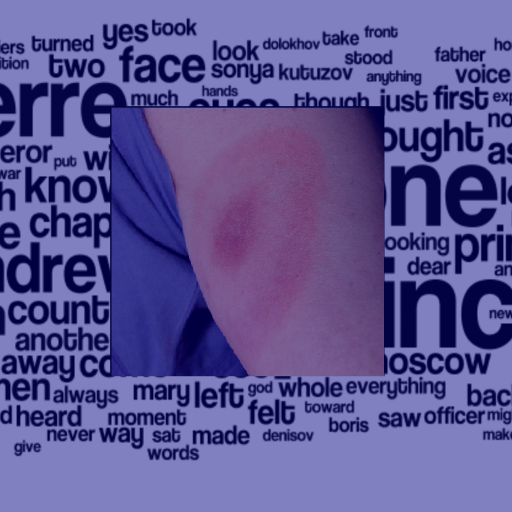
\includegraphics[width=.12\textheight ,keepaspectratio]{images/pretraining/gradcam/3/VGG16CombinedGradCam.png} &
			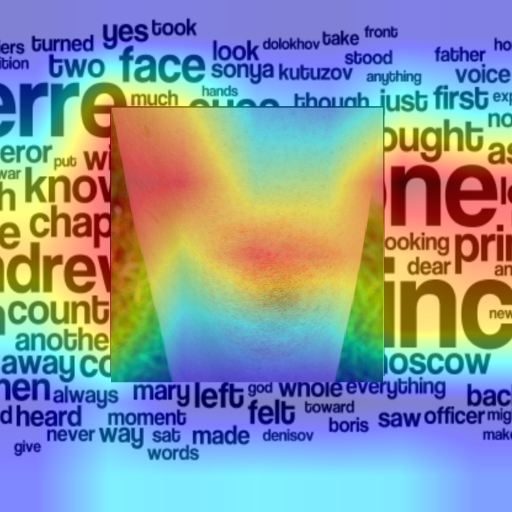
\includegraphics[width=.12\textheight ,keepaspectratio]{images/pretraining/gradcam/9/VGG16CombinedGradCam.png} &
			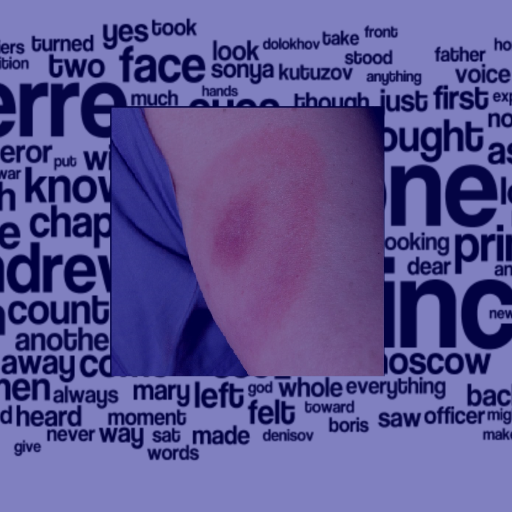
\includegraphics[width=.12\textheight ,keepaspectratio]{images/pretraining/gradcam/3/VGG19CombinedGradCam.png} &
			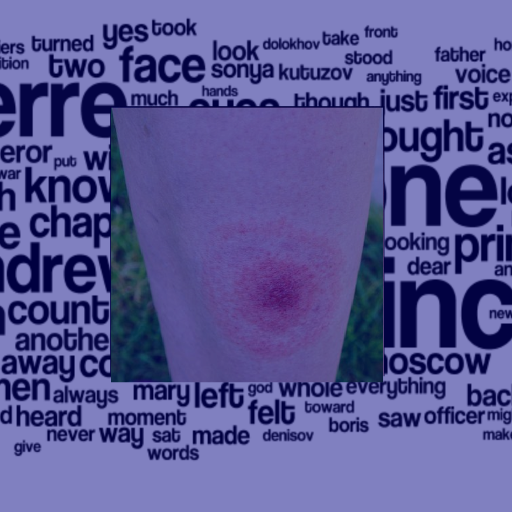
\includegraphics[width=.12\textheight ,keepaspectratio]{images/pretraining/gradcam/9/VGG19CombinedGradCam.png} &
			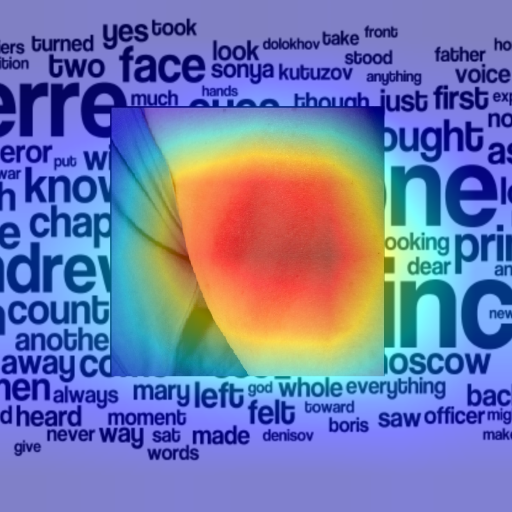
\includegraphics[width=.12\textheight ,keepaspectratio]{images/pretraining/gradcam/3/ResNet50CombinedGradCam.png} &
			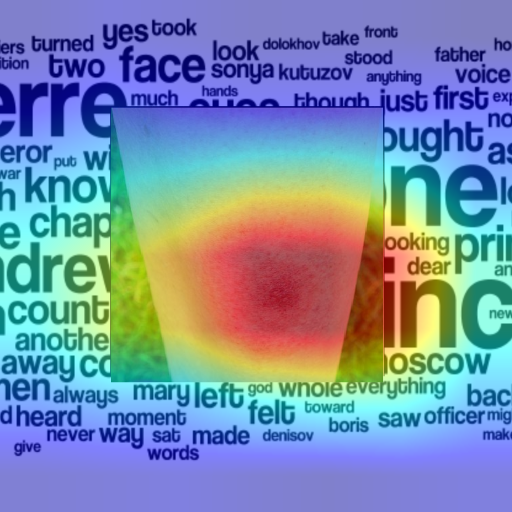
\includegraphics[width=.12\textheight ,keepaspectratio]{images/pretraining/gradcam/9/ResNet50CombinedGradCam.png} &
			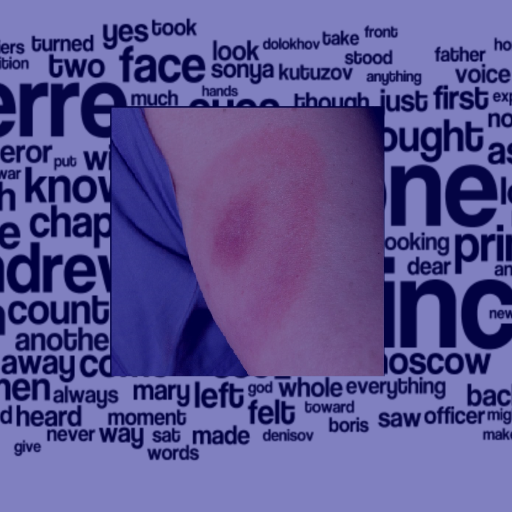
\includegraphics[width=.12\textheight ,keepaspectratio]{images/pretraining/gradcam/3/ResNet101CombinedGradCam.png} &
			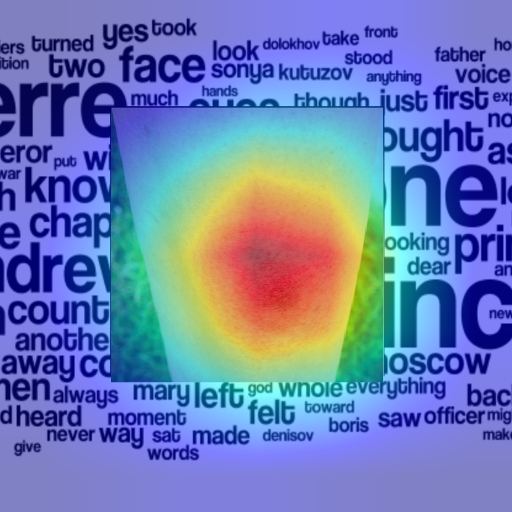
\includegraphics[width=.12\textheight ,keepaspectratio]{images/pretraining/gradcam/9/ResNet101CombinedGradCam.png} &
			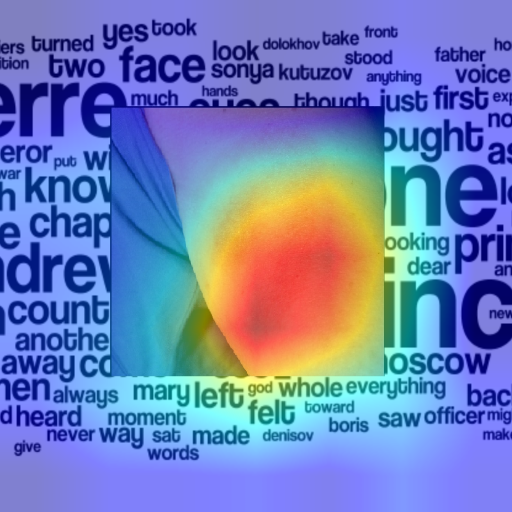
\includegraphics[width=.12\textheight ,keepaspectratio]{images/pretraining/gradcam/3/ResNet50V2CombinedGradCam.png} &
			\includegraphics[width=.12\textheight ,keepaspectratio]{images/pretraining/gradcam/9/ResNet50V2CombinedGradCam.png}
			\\\cmidrule(lr){1-10}
			
			\multicolumn{2}{c}{ResNet101V2-233} & \multicolumn{2}{c}{InceptionV3-274} & \multicolumn{2}{c}{InceptionV4-327} & \multicolumn{2}{c}{InceptionResNetV2-500} & \multicolumn{2}{c}{Xception-118}\\
			\includegraphics[width=.12\textheight ,keepaspectratio]{images/pretraining/gradcam/3/ResNet101V2CombinedGradCam.png} &
			\includegraphics[width=.12\textheight ,keepaspectratio]{images/pretraining/gradcam/9/ResNet101V2CombinedGradCam.png} &
			\includegraphics[width=.12\textheight ,keepaspectratio]{images/pretraining/gradcam/3/InceptionV3CombinedGradCam.png} &
			\includegraphics[width=.12\textheight ,keepaspectratio]{images/pretraining/gradcam/9/InceptionV3CombinedGradCam.png} &
			\includegraphics[width=.12\textheight ,keepaspectratio]{images/pretraining/gradcam/3/InceptionV4CombinedGradCam.png} &
			\includegraphics[width=.12\textheight ,keepaspectratio]{images/pretraining/gradcam/9/InceptionV4CombinedGradCam.png} &
			\includegraphics[width=.12\textheight ,keepaspectratio]{images/pretraining/gradcam/3/InceptionResNetV2CombinedGradCam.png} &
			\includegraphics[width=.12\textheight ,keepaspectratio]{images/pretraining/gradcam/9/InceptionResNetV2CombinedGradCam.png} &
			\includegraphics[width=.12\textheight ,keepaspectratio]{images/pretraining/gradcam/3/XceptionCombinedGradCam.png} &
			\includegraphics[width=.12\textheight ,keepaspectratio]{images/pretraining/gradcam/9/XceptionCombinedGradCam.png}
			\\\cmidrule(lr){1-10}
			
			\multicolumn{2}{c}{DenseNet121-379} & \multicolumn{2}{c}{DenseNet169-395} & \multicolumn{2}{c}{DenseNet201-561} & \multicolumn{2}{c}{MobileNetV2-62} & \multicolumn{2}{c}{MobileNetV3Small-182}\\
			\includegraphics[width=.12\textheight ,keepaspectratio]{images/pretraining/gradcam/3/DenseNet121CombinedGradCam.png} &
			\includegraphics[width=.12\textheight ,keepaspectratio]{images/pretraining/gradcam/9/DenseNet121CombinedGradCam.png} &
			\includegraphics[width=.12\textheight ,keepaspectratio]{images/pretraining/gradcam/3/DenseNet169CombinedGradCam.png} &
			\includegraphics[width=.12\textheight ,keepaspectratio]{images/pretraining/gradcam/9/DenseNet169CombinedGradCam.png} &
			\includegraphics[width=.12\textheight ,keepaspectratio]{images/pretraining/gradcam/3/DenseNet201CombinedGradCam.png} &
			\includegraphics[width=.12\textheight ,keepaspectratio]{images/pretraining/gradcam/9/DenseNet201CombinedGradCam.png} &
			\includegraphics[width=.12\textheight ,keepaspectratio]{images/pretraining/gradcam/3/MobileNetV2CombinedGradCam.png} &
			\includegraphics[width=.12\textheight ,keepaspectratio]{images/pretraining/gradcam/9/MobileNetV2CombinedGradCam.png} &
			\includegraphics[width=.12\textheight ,keepaspectratio]{images/pretraining/gradcam/3/MobileNetV3SmallCombinedGradCam.png} &
			\includegraphics[width=.12\textheight ,keepaspectratio]{images/pretraining/gradcam/9/MobileNetV3SmallCombinedGradCam.png}
			\\\cmidrule(lr){1-10}
			
			\multicolumn{2}{c}{MobileNetV3Large-193} & \multicolumn{2}{c}{NASNetMobile-617} & \multicolumn{2}{c}{EfficientNetB0-187} & \multicolumn{2}{c}{EfficientNetB1-308} & \multicolumn{2}{c}{EfficientNetB2-316}\\
			\includegraphics[width=.12\textheight ,keepaspectratio]{images/pretraining/gradcam/3/MobileNetV3LargeCombinedGradCam.png} &
			\includegraphics[width=.12\textheight ,keepaspectratio]{images/pretraining/gradcam/9/MobileNetV3LargeCombinedGradCam.png} &
			\includegraphics[width=.12\textheight ,keepaspectratio]{images/pretraining/gradcam/3/NASNetMobileCombinedGradCam.png} &
			\includegraphics[width=.12\textheight ,keepaspectratio]{images/pretraining/gradcam/9/NASNetMobileCombinedGradCam.png} &
			\includegraphics[width=.12\textheight ,keepaspectratio]{images/pretraining/gradcam/3/EfficientNetB0CombinedGradCam.png} &
			\includegraphics[width=.12\textheight ,keepaspectratio]{images/pretraining/gradcam/9/EfficientNetB0CombinedGradCam.png} &
			\includegraphics[width=.12\textheight ,keepaspectratio]{images/pretraining/gradcam/3/EfficientNetB1CombinedGradCam.png} &
			\includegraphics[width=.12\textheight ,keepaspectratio]{images/pretraining/gradcam/9/EfficientNetB1CombinedGradCam.png} &
			\includegraphics[width=.12\textheight ,keepaspectratio]{images/pretraining/gradcam/3/EfficientNetB2CombinedGradCam.png} &
			\includegraphics[width=.12\textheight ,keepaspectratio]{images/pretraining/gradcam/9/EfficientNetB2CombinedGradCam.png}
			\\\cmidrule(lr){1-10}
			
			\multicolumn{2}{c}{EfficientNetB3-194} & \multicolumn{2}{c}{EfficientNetB4-384} & \multicolumn{2}{c}{EfficientNetB5-444} & \multicolumn{2}{c}{EfficientNetV2S-413} & \multicolumn{2}{c}{ConvNeXtTiny-120}\\
			\includegraphics[width=.12\textheight ,keepaspectratio]{images/pretraining/gradcam/3/EfficientNetB3CombinedGradCam.png} &
			\includegraphics[width=.12\textheight ,keepaspectratio]{images/pretraining/gradcam/9/EfficientNetB3CombinedGradCam.png} &
			\includegraphics[width=.12\textheight ,keepaspectratio]{images/pretraining/gradcam/3/EfficientNetB4CombinedGradCam.png} &
			\includegraphics[width=.12\textheight ,keepaspectratio]{images/pretraining/gradcam/9/EfficientNetB4CombinedGradCam.png} &
			\includegraphics[width=.12\textheight ,keepaspectratio]{images/pretraining/gradcam/3/EfficientNetB5CombinedGradCam.png} &
			\includegraphics[width=.12\textheight ,keepaspectratio]{images/pretraining/gradcam/9/EfficientNetB5CombinedGradCam.png} &
			\includegraphics[width=.12\textheight ,keepaspectratio]{images/pretraining/gradcam/3/ENV2SCombinedGradCam.png} &
			\includegraphics[width=.12\textheight ,keepaspectratio]{images/pretraining/gradcam/9/ENV2SCombinedGradCam.png} &
			\includegraphics[width=.12\textheight ,keepaspectratio]{images/pretraining/gradcam/3/ConvNextTinyCombinedGradCam.png} &
			\includegraphics[width=.12\textheight ,keepaspectratio]{images/pretraining/gradcam/9/ConvNextTinyCombinedGradCam.png} \\\bottomrule
		\end{tabular}
		%		\\\cmidrule(lr){1-10}
	\end{table}
\end{landscape}
%%%%%%%%%%%%GRADCAM%%%%%%%%%%%%%%%%%%%%%%


	%%%%%%%%%%%%%%%%%%%%%%%%%%%%%%%%%%%%%%%%%%%%%%%%%%%%%%%%%%%%%%%%%%%%%%%%
\chapter{Expert Opinion Elicitation for Assisting Lesion Image Classifier With Patient Data}\label{chap:Elicitation}\chaptermark{Expert Opinion Elicitation}
%%%%%%%%%%%%%%%%%%%%%%%%%%%%%%%%%%%%%%%%%%%%%%%%%%%%%%%%%%%%%%%%%%%%%%%%

\begin{center}
	\begin{minipage}{0.8\textwidth}
		\begin{small}
			This chapter addresses research question \ref{question2}, presents our questionnaire based expert opinion elicitation method for calculating disease probability from patient data and an approach for combining independent probability estimates from multiple modalities. Contents from this chapter have been used in the following article:
			\begin{itemize}
				\item \fullcite{Hossain2022Elicitation}
			\end{itemize}  
		\end{small}
	\end{minipage}
	\vspace{0.5cm}
\end{center}

\minitoc

%%%%%%%%%%%%%%%%%%%%%%%%%%%%%%%%%%%%%%%%%%%%%%%%%%%%%%%%%%%%%%%%%%%%%%%%
\section{Introduction}
%%%%%%%%%%%%%%%%%%%%%%%%%%%%%%%%%%%%%%%%%%%%%%%%%%%%%%%%%%%%%%%%%%%%%%%%
When the dermatologists rechecked the annotations of the Lyme image dataset misclassified by most of the convolutional neural networks (CNNs) (discussed in Chapter \ref{chap:Pretraining}) they found mistakes in some of the initial annotations. This suggests that some images are too confusing to classify even for the experts without additional context from patient data.

Expert opinion elicitation can be effective when high quality data is difficult to collect \cite{Wilson2018}. Point estimates (such as medians or means), intervals of uncertainty (such as confidence intervals or quartiles), or probability distributions can all be included in the measurements elicited \cite{cadham2022use}. Expert opinion elicitation and aggregation processes can be classified into two categories: behavioral and mathematical approaches \cite{Clemen1999, cadham2022use}. The behavioral approach tries to produce group consensus among experts whereas, the mathematical approach combines subjective probabilities from experts using mathematical methods (some form of averaging) \cite{cadham2022use}.

Expert elicitation proved effective for medical diagnosis and decision making. For example, Van Der Gaag et al. \cite{VanDerGaag2002} created a probabilistic network to describe the oesophageal cancer presentation characteristics and the pathophysiological mechanisms of invasion and metastasis by eliciting opinions from two experts. Saegerman et al. \cite{Saegerman2022} elicited opinions from eleven European experts to rank the drivers of the emergence of bovine besnoitiosis a chronic disease in cattle.  Wilson et al. \cite{Wilson2018} elicited opinions from sixteen experts on the disease progression probability in patients with untreated melanoma. The article by Cadham et al. \cite{cadham2022use} contains a detailed review of the application of expert elicitation in health research computational modeling studies.

In our study, for the first time, we elicited opinions from fifteen expert dermatologists to create a model for calculating erythema migrans (EM) probability from patient data as an early symptom of Lyme disease. First, with the help of the experts, a questionnaire was prepared based on questions that the doctors ask during EM diagnosis. The traditional expert elicitation process of collecting probability estimates for cases based on the questionnaire is time consuming and it is difficult for doctors to provide probability estimates for cases or distribution parameters. Therefore, we opted for a more relaxed approach of relative weight assignment to different answers to the questions and converted the doctor’s evaluations to EM probabilities utilizing Gaussian mixture model (GMM) based density estimation (described in Section \ref{sec:GMM}). To validate the elicited probability model and explain its behavior to the experts we utilized formal concept analysis (described in Section \ref{sec:FCA}) and decision tree (described in Section \ref{sec:DecTree}). The elicited patient data based EM probability model will be useful for assisting image-based EM classifiers with additional context from patient data. We also proposed an algorithm for combining the EM probability score from a deep learning image classifier with the elicited probability score from patient data. The proposed algorithm ensures veto power for the patient data. The elicited probability score and the proposed algorithm can be utilized to make image based deep learning Lyme disease pre-scanners robust and the techniques will be useful for questionnaire based opinion elicitation of other diseases.

The rest of the chapter is structured as follows: Section \ref{sec:elicitation} describes the expert elicitation process and elicitation result; Section \ref{sec:combining_prob} contains the strategy for combining probabilities; finally, Section \ref{sec:elicitation_conclusion} provides concluding remarks.

\section{Elicitation Method}\label{sec:elicitation}
The details of our expert elicitation process like expert recruitment, questionnaire preparation, experts’ opinion collection, elicitation methods, result, and analysis are presented in the following subsections.

\subsection{Expert Selection}
The recruited experts are hospital practitioners who are infectious disease specialists or dermatologists working in reference centers for tick-borne diseases of France - Centres de Référence des Maladies Vectorielles liées aux Tiques (CRMVT) \cite{CRMVTRef}. At a CRMVT steering committee meeting held in June 2021 with participants from all the reference centers, Professor Olivier Lesens (Infectious and Tropical Diseases Department, CRIOA, CHU Clermont-Ferrand, France) explained the importance of expert elicitation for calculating EM probability based on patient data and requested the interested experts to participate in the elicitation process. Fifteen experts agreed to participate\footnote{The experts did not receive any monetary benefits for participating in the elicitation process.}. Table \ref{tab:expert_table} lists the reference centers and the corresponding number of experts participating in the elicitation process.
\begin{table}[tb!]
	\caption{Experts recruited for erythema migrans probability elicitation.}
	\label{tab:expert_table}
	\resizebox{\textwidth}{!}{%
		\begin{tabular}{lc}
			\toprule
			\multicolumn{1}{c}{\textbf{Center}} &
			\textbf{Number of Participating Experts} \\ \midrule
			\begin{tabular}[c]{l}\textbf{CRMVT du Grand Ouest}\\ Hôpital Pontchaillou  \\ Centre Urgences-Réanimations \\ 2 rue Henri Le Guilloux \\ 35033 Rennes Cedex 09\end{tabular} &
			2 \\ \cmidrule(lr){1-2}
			\begin{tabular}[c]{l}\textbf{CRMVT Ile-de-France et Hauts-de-France} \\ Hôpital de Villeneuve-Saint-Georges \\ Secrétariat du centre Lyme \\ 40 allée de la Source \\ 94195 Villeneuve-Saint-Georges Cedex\end{tabular} &
			2 \\ \cmidrule(lr){1-2}
			\begin{tabular}[c]{l}\textbf{CRMVT de Strasbourg} \\ Nouvel Hôpital Civil - Hôpitaux Universitaires de Strasbourg (HUS) \\ 1 place de l'Hôpital BP461 \\ 67091 STRASBOURG Cedex\end{tabular} &
			1 \\ \cmidrule(lr){1-2}
			\begin{tabular}[c]{l}\textbf{CRMVT de Nancy} \\ Centre Hospitalier Régional et Universitaire \\ (CHRU) de Nancy \\ Rue du Morvan \\ 54500 Vandœuvre-lès-Nancy\end{tabular} &
			1 \\ \cmidrule(lr){1-2}
			\begin{tabular}[c]{l}\textbf{CRMVT de Clermont-Ferrand} \\ Service des Maladies Infectieuses et Tropicales \\ CHU Gabriel Montpied \\ 58, Rue Montalembert \\ 63003 Clermont-Ferrand Cedex 1\end{tabular} &
			8 \\ \cmidrule(lr){1-2}
			\begin{tabular}[c]{l}\textbf{CRMVT de Saint-Etienne} \\ Service des Maladies Infectieuses et Tropicales Hôpital Nord \\ Avenue Albert Raimond \\ 42270 Saint-Priest-en-Jarez\end{tabular} &
			1 \\ \bottomrule
		\end{tabular}%
	}
\end{table}

\subsection{Questionnaire and Experts’ Evaluation}
For the EM probability elicitation, a questionnaire was prepared based on questions about the context of onset and progression of the skin lesion that a physician usually asks when diagnosing EM. The questionnaire is based on a previous study concerning the collection of EM related data from rural areas of France \cite{Letertre-Gibert2020}. The questionnaire was finalized through several meetings held in April 2020 among the doctors of CRMVT in Clermont-Ferrand and experts in tick ecology from the French national research institute for agriculture, food and the environment - \selectlanguage{french}Institut national de recherche pour l'agriculture, l'alimentation et l'environnement (INRAE) \selectlanguage{english}\cite{INRAE}. Experts who volunteered to participate in the elicitation process at the meeting in June 2021 agreed that there were many possible cases from the combination of the questions and answers, and it was time consuming and difficult for them to provide probability estimates for all those different cases. Therefore, experts agreed to independently assign relative weights to different possible answers associated with each question. The assigned weight values are in the range $-1$ to $+3$ (a higher value represents a higher contribution of the answer towards the possibility of the EM). The experts were contacted via email with detailed instructions to provide their weight attributions independently. Table \ref{tab:initial_opinion} lists the questions, answers, and weight attribution from the doctors.
\begin{table}[tb!]
	\caption[Questionnaire and doctors’ weight attribution for erythema migrans]{Questionnaire and doctors’ weight attribution for erythema migrans. The assigned weight values are in the range $-1$ to $+3$ (a higher value represents a higher contribution of the answer towards the possibility of the erythema migrans). $d_{1}$ to $d_{15}$ represents the doctors.}
	\label{tab:initial_opinion}
	\resizebox{\textwidth}{!}{%
		\begin{tabular}{cllcccccccccccccccc}
			\toprule
			\multirow{2}{*}{\textbf{Question}} &
			\multicolumn{2}{c}{\multirow{2}{*}{\textbf{Answer}}} &
			\multicolumn{16}{c}{\textbf{\begin{tabular}[c]{@{}c@{}}Weight Assigned by Doctors \\ (Doctor's Evaluation)\end{tabular}}} \\ \cmidrule(l){4-19} 
			&
			\multicolumn{2}{c}{} &
			$d_{1}$ &
			$d_{2}$ &
			$d_{3}$ &
			$d_{4}$ &
			$d_{5}$ &
			$d_{6}$ &
			$d_{7}$ &
			$d_{8}$ &
			$d_{9}$ &
			$d_{10}$ &
			$d_{11}$ &
			$d_{12}$ &
			$d_{13}$ &
			$d_{14}$ &
			$d_{15}$ &
			Average \\ \midrule \addlinespace[2pt]
			\multirow{7}{*}[-2.7em]{\begin{tabular}[c]{@{}c@{}}Other symptoms observed \\ alongside the skin lesion\end{tabular}} &
			\multicolumn{2}{l}{No} &
			0 &
			0 &
			3 &
			0 &
			0 &
			1 &
			2 &
			1 &
			2 &
			1 &
			2 &
			1 &
			1 &
			2 &
			3 &
			1.27 \\ \addlinespace[2pt] \cmidrule(lr) {2-19} \addlinespace[2pt]
			&
			\multicolumn{2}{l}{Fever} &
			-1 &0 &-1 &1 &1 &1 &1 &1 &1 &1 &1 &1 &1 &1 &0 &0.6 \\ \addlinespace[2pt] \cmidrule(lr){2-19} \addlinespace[2pt]
			&
			\multicolumn{2}{l}{Fatigue} &
			0 &1 &1 &2 &0 &0 &1 &1 &1 &1 &1 &0 &1 &0 &0 &0.67 \\ \addlinespace[2pt] \cmidrule(lr){2-19} \addlinespace[2pt]
			&
			\multicolumn{2}{l}{Faintness} &
			0 &0 &1 &0 &0 &0 &0 &0 &1 &0 &1 &-1 &1 &0 &0 &0.2 \\ \addlinespace[2pt] \cmidrule(lr){2-19} \addlinespace[2pt]
			&
			\multicolumn{2}{l}{Joint pain} &
			0 &0 &-1 &0 &2 &0 &1 &1 &0 &2 &1 &1 &1 &0 &0 &0.53 \\ \addlinespace[2pt] \cmidrule(lr){2-19} \addlinespace[2pt]
			&
			\multicolumn{2}{l}{Headache} &
			1 &
			1 &
			-1 &
			2 &
			2 &
			1 &
			1 &
			1 &
			1 &
			1 &
			1 &
			1 &
			1 &
			0 &
			0 &
			0.87 \\ \addlinespace[2pt] \cmidrule(lr){2-19} \addlinespace[2pt]
			&
			\multicolumn{2}{l}{Itching} &
			-1 &
			-1 &
			-1 &
			-1 &
			1 &
			-1 &
			0 &
			0 &
			0 &
			1 &
			-0.5 &
			-1 &
			-1 &
			1 &
			0 &
			-0.3 \\ \addlinespace[2pt] \cmidrule(lr){1-19} \addlinespace[2pt]
			\multirow{4}{*}[-1.5em]{\begin{tabular}[c]{@{}c@{}}What was the maximum \\ size of the red rash\end{tabular}} &
			\multicolumn{2}{l}{$<1$ cm} &
			-1 &
			-1 &
			0 &
			-1 &
			-1 &
			-1 &
			-1 &
			0 &
			0 &
			-1 &
			-1 &
			-1 &
			-1 &
			1 &
			-1 &
			-0.67 \\ \addlinespace[2pt] \cmidrule(lr){2-19} \addlinespace[2pt]
			&
			\multicolumn{2}{l}{1 to 5 cm} &
			1 &
			1 &
			1 &
			0 &
			1 &
			0 &
			1 &
			1 &
			2 &
			1 &
			1 &
			1 &
			1 &
			2 &
			1 &
			1 \\ \addlinespace[2pt] \cmidrule(lr){2-19} \addlinespace[2pt]
			&
			\multicolumn{2}{l}{$>5$ cm} &
			3 &
			2 &
			2 &
			2 &
			3 &
			2 &
			3 &
			2 &
			1 &
			3 &
			2 &
			2 &
			3 &
			3 &
			3 &
			2.4 \\ \addlinespace[2pt] \cmidrule(lr){2-19} \addlinespace[2pt]
			&
			\multicolumn{2}{l}{I do not know} &
			0 &
			0 &
			0 &
			0 &
			0 &
			0 &
			-1 &
			1 &
			0 &
			0 &
			0 &
			0 &
			0 &
			0 &
			0 &
			0 \\ \addlinespace[2pt] \cmidrule(lr){1-19} \addlinespace[2pt]
			\multirow{3}{*}[-1em]{\begin{tabular}[c]{@{}c@{}}Is the size of the red rash \\ increasing or has it \\ gradually increased\end{tabular}} &
			\multicolumn{2}{l}{Yes} &
			3 &
			1 &
			3 &
			3 &
			3 &
			3 &
			3 &
			3 &
			2 &
			3 &
			3 &
			3 &
			3 &
			3 &
			3 &
			2.8 \\ \addlinespace[2pt] \cmidrule(lr){2-19} \addlinespace[2pt]
			&
			\multicolumn{2}{l}{No} &
			0 &
			-1 &
			-1 &
			-1 &
			-1 &
			-1 &
			-1 &
			0 &
			-1 &
			0 &
			-1 &
			-1 &
			-1 &
			1 &
			-1 &
			-0.67 \\ \addlinespace[2pt] \cmidrule(lr){2-19} \addlinespace[2pt]
			&
			\multicolumn{2}{l}{I do not know} &
			0 &
			0 &
			0 &
			0 &
			0 &
			0 &
			0 &
			1 &
			0 &
			0 &
			0 &
			0 &
			0 &
			0 &
			0 &
			0.07 \\ \addlinespace[2pt] \cmidrule(lr){1-19} \addlinespace[2pt]
			\multirow{2}{*}{\begin{tabular}[c]{@{}c@{}}Have you seen a tick bite \\on this red rash \\in the past 30 days\end{tabular}} &
			\multicolumn{2}{l}{Yes} &
			3 &
			2 &
			3 &
			2 &
			3 &
			1 &
			3 &
			3 &
			2 &
			3 &
			2 &
			3 &
			1 &
			3 &
			3 &
			2.47 \\ \addlinespace[4pt] \cmidrule(lr){2-19} \addlinespace[2pt]
			&
			\multicolumn{2}{l}{No} &
			0 &
			0 &
			0 &
			0 &
			0 &
			1 &
			0 &
			1 &
			0 &
			0 &
			-0.5 &
			-1 &
			0 &
			1 &
			0 &
			0.1 \\ \addlinespace[2pt] \cmidrule(lr){1-19} \addlinespace[2pt]
			\multirow{4}{*}[-1.5em]{\begin{tabular}[c]{@{}c@{}}Frequency of tick bites \\in the last 30 days \\before the appearance \\ of the red rash\end{tabular}} &
			\multicolumn{2}{l}{Never} &
			-1 &
			-1 &
			0 &
			0 &
			-1 &
			0 &
			0 &
			0 &
			0 &
			0 &
			-1 &
			-1 &
			0 &
			-1 &
			0 &
			-0.4 \\ \addlinespace[2pt] \cmidrule(lr){2-19} \addlinespace[2pt]
			&
			\multicolumn{2}{l}{1 time} &
			0 &
			0 &
			2 &
			1 &
			1 &
			1 &
			1 &
			1 &
			2 &
			1 &
			1 &
			1 &
			1 &
			2 &
			1 &
			1.07 \\ \addlinespace[2pt] \cmidrule(lr){2-19} \addlinespace[2pt]
			&
			\multicolumn{2}{l}{2 to 5 times} &
			1 &
			1 &
			3 &
			1 &
			1 &
			1 &
			1 &
			2 &
			2 &
			1 &
			2 &
			1 &
			1 &
			3 &
			1 &
			1.47 \\ \addlinespace[2pt] \cmidrule(lr){2-19} \addlinespace[2pt]
			&
			\multicolumn{2}{l}{$>5$ times} &
			2 &
			2 &
			1 &
			2 &
			2 &
			1 &
			1 &
			2 &
			2 &
			2 &
			3 &
			1 &
			1 &
			3 &
			2 &
			1.8 \\ \addlinespace[2pt] \cmidrule(lr){1-19} \addlinespace[2pt]
			\multirow{2}{*}{\begin{tabular}[c]{@{}c@{}}Outdoor activities in the \\last  30 days before the \\onset of the red rash\end{tabular}} &
			\multicolumn{2}{l}{Yes} &
			1 &
			1 &
			2 &
			2 &
			1 &
			1 &
			2 &
			2 &
			2 &
			2 &
			2 &
			2 &
			1 &
			3 &
			2 &
			1.73 \\ \addlinespace[2pt] \cmidrule(lr){2-19} \addlinespace[2pt]
			&
			\multicolumn{2}{l}{No} &
			-1 &
			-1 &
			-1 &
			-1 &
			-1 &
			0 &
			-1 &
			1 &
			-1 &
			-1 &
			-1 &
			-1 &
			0 &
			-1 &
			0 &
			-0.67 \\\addlinespace[5pt] \bottomrule
		\end{tabular}%
	}
\end{table}
After receiving the weight attributions from all the experts, they participated in a meeting in November 2021 and agreed that fever, fatigue, faintness, and headache should contribute equally if one or more of these answers were present and the contribution should be the average of these four answers. Therefore, the four answers were replaced with one, and the possible cases reduced to 1,536 from 12,288 cases. This modification is shown in Table \ref{tab:modified_opinion}.
\begin{table}[tb!]
	\caption[Weight modified questionnaire and doctors’ weight attribution for erythema migrans]{Weight modified questionnaire and doctors’ weight attribution for erythema migrans. The assigned weight values are in the range $-1$ to $+3$ (a higher value represents a higher contribution of the answer towards the possibility of the erythema migrans). $d_{1}$ to $d_{15}$ represents the doctors.}
	\label{tab:modified_opinion}
	\resizebox{\textwidth}{!}{%
		\begin{tabular}{cllcccccccccccccccc}
			\toprule
			\multirow{2}{*}{\textbf{Question}} &
			\multicolumn{2}{c}{\multirow{2}{*}{\textbf{Answer}}} &
			\multicolumn{16}{c}{\textbf{\begin{tabular}[c]{@{}c@{}}Weight Assigned by Doctors \\ (Doctor's Evaluation)\end{tabular}}} \\ \cmidrule(l){4-19} 
			&
			\multicolumn{2}{c}{} &
			$d_{1}$ &
			$d_{2}$ &
			$d_{3}$ &
			$d_{4}$ &
			$d_{5}$ &
			$d_{6}$ &
			$d_{7}$ &
			$d_{8}$ &
			$d_{9}$ &
			$d_{10}$ &
			$d_{11}$ &
			$d_{12}$ &
			$d_{13}$ &
			$d_{14}$ &
			$d_{15}$ &
			Average \\ \midrule \addlinespace[2pt]
			\multirow{4}{*}[-2.7em]{\begin{tabular}[c]{@{}c@{}}Other symptoms observed \\ alongside the skin lesion $(q_{1})$\end{tabular}} &
			\multicolumn{2}{l}{No $(a_{1,q_{1}})$} &
			0 &
			0 &
			3 &
			0 &
			0 &
			1 &
			2 &
			1 &
			2 &
			1 &
			2 &
			1 &
			1 &
			2 &
			3 &
			1.27 \\ \addlinespace[2pt] \cmidrule(lr) {2-19} \addlinespace[2pt]
			&
			\multicolumn{2}{l}{\begin{tabular}[c]{@{}l@{}}Fever/\\ Fatigue/\\ Faintness/\\ Headache $(a_{2,q_{1}})$\end{tabular}} &
			\rotatebox[origin=c]{90}{-0.25} &
			\rotatebox[origin=c]{90}{0.25} &
			\rotatebox[origin=c]{90}{0} &
			\rotatebox[origin=c]{90}{0.75} &
			\rotatebox[origin=c]{90}{0.75} &
			\rotatebox[origin=c]{90}{0.25} &
			\rotatebox[origin=c]{90}{0.75} &
			\rotatebox[origin=c]{90}{0.75} &
			\rotatebox[origin=c]{90}{0.75} &
			\rotatebox[origin=c]{90}{1} &
			\rotatebox[origin=c]{90}{1} &
			\rotatebox[origin=c]{90}{0.25} &
			\rotatebox[origin=c]{90}{1} &
			\rotatebox[origin=c]{90}{0.25} &
			\rotatebox[origin=c]{90}{0} &
			\rotatebox[origin=c]{90}{0.5} \\ \addlinespace[2pt] \cmidrule(lr){2-19} \addlinespace[2pt]
			&
			\multicolumn{2}{l}{Joint pain $(a_{3,q_{1}})$} &
			1 &
			1 &
			-1 &
			2 &
			2 &
			1 &
			1 &
			1 &
			1 &
			1 &
			1 &
			1 &
			1 &
			0 &
			0 &
			0.87 \\ \addlinespace[2pt] \cmidrule(lr){2-19} \addlinespace[2pt]
			&
			\multicolumn{2}{l}{Itching $(a_{4,q_{1}})$} &
			-1 &
			-1 &
			-1 &
			-1 &
			1 &
			-1 &
			0 &
			0 &
			0 &
			1 &
			-0.5 &
			-1 &
			-1 &
			1 &
			0 &
			-0.3 \\ \addlinespace[2pt] \cmidrule(lr){1-19} \addlinespace[2pt]
			\multirow{4}{*}[-1.5em]{\begin{tabular}[c]{@{}c@{}}What was the maximum \\ size of the red rash $(q_{2})$\end{tabular}} &
			\multicolumn{2}{l}{$<1$ cm $(a_{1,q_{2}})$} &
			-1 &
			-1 &
			0 &
			-1 &
			-1 &
			-1 &
			-1 &
			0 &
			0 &
			-1 &
			-1 &
			-1 &
			-1 &
			1 &
			-1 &
			-0.67 \\ \addlinespace[2pt] \cmidrule(lr){2-19} \addlinespace[2pt]
			&
			\multicolumn{2}{l}{1 to 5 cm $(a_{2,q_{2}})$} &
			1 &
			1 &
			1 &
			0 &
			1 &
			0 &
			1 &
			1 &
			2 &
			1 &
			1 &
			1 &
			1 &
			2 &
			1 &
			1 \\ \addlinespace[2pt] \cmidrule(lr){2-19} \addlinespace[2pt]
			&
			\multicolumn{2}{l}{$>5$ cm $(a_{3,q_{2}})$} &
			3 &
			2 &
			2 &
			2 &
			3 &
			2 &
			3 &
			2 &
			1 &
			3 &
			2 &
			2 &
			3 &
			3 &
			3 &
			2.4 \\ \addlinespace[2pt] \cmidrule(lr){2-19} \addlinespace[2pt]
			&
			\multicolumn{2}{l}{I do not know $(a_{4,q_{2}})$} &
			0 &
			0 &
			0 &
			0 &
			0 &
			0 &
			-1 &
			1 &
			0 &
			0 &
			0 &
			0 &
			0 &
			0 &
			0 &
			0 \\ \addlinespace[2pt] \cmidrule(lr){1-19} \addlinespace[2pt]
			\multirow{3}{*}[-1em]{\begin{tabular}[c]{@{}c@{}}Is the size of the red rash \\ increasing or has it \\ gradually increased  $(q_{3})$\end{tabular}} &
			\multicolumn{2}{l}{Yes $(a_{1,q_{3}})$} &
			3 &
			1 &
			3 &
			3 &
			3 &
			3 &
			3 &
			3 &
			2 &
			3 &
			3 &
			3 &
			3 &
			3 &
			3 &
			2.8 \\ \addlinespace[2pt] \cmidrule(lr){2-19} \addlinespace[2pt]
			&
			\multicolumn{2}{l}{No $(a_{2,q_{3}})$} &
			0 &
			-1 &
			-1 &
			-1 &
			-1 &
			-1 &
			-1 &
			0 &
			-1 &
			0 &
			-1 &
			-1 &
			-1 &
			1 &
			-1 &
			-0.67 \\ \addlinespace[2pt] \cmidrule(lr){2-19} \addlinespace[2pt]
			&
			\multicolumn{2}{l}{I do not know $(a_{3,q_{3}})$} &
			0 &
			0 &
			0 &
			0 &
			0 &
			0 &
			0 &
			1 &
			0 &
			0 &
			0 &
			0 &
			0 &
			0 &
			0 &
			0.07 \\ \addlinespace[2pt] \cmidrule(lr){1-19} \addlinespace[2pt]
			\multirow{2}{*}{\begin{tabular}[c]{@{}c@{}}Have you seen a tick bite \\on this red rash \\in the past 30 days $(q_{4})$\end{tabular}} &
			\multicolumn{2}{l}{Yes $(a_{1,q_{4}})$} &
			3 &
			2 &
			3 &
			2 &
			3 &
			1 &
			3 &
			3 &
			2 &
			3 &
			2 &
			3 &
			1 &
			3 &
			3 &
			2.47 \\ \addlinespace[4pt] \cmidrule(lr){2-19} \addlinespace[2pt]
			&
			\multicolumn{2}{l}{No $(a_{2,q_{4}})$} &
			0 &
			0 &
			0 &
			0 &
			0 &
			1 &
			0 &
			1 &
			0 &
			0 &
			-0.5 &
			-1 &
			0 &
			1 &
			0 &
			0.1 \\ \addlinespace[2pt] \cmidrule(lr){1-19} \addlinespace[2pt]
			\multirow{4}{*}[-1.5em]{\begin{tabular}[c]{@{}c@{}}Frequency of tick bites \\in the last 30 days \\before the appearance \\ of the red rash $(q_{5})$\end{tabular}} &
			\multicolumn{2}{l}{Never $(a_{1,q_{5}})$} &
			-1 &
			-1 &
			0 &
			0 &
			-1 &
			0 &
			0 &
			0 &
			0 &
			0 &
			-1 &
			-1 &
			0 &
			-1 &
			0 &
			-0.4 \\ \addlinespace[2pt] \cmidrule(lr){2-19} \addlinespace[2pt]
			&
			\multicolumn{2}{l}{1 time $(a_{2,q_{5}})$} &
			0 &
			0 &
			2 &
			1 &
			1 &
			1 &
			1 &
			1 &
			2 &
			1 &
			1 &
			1 &
			1 &
			2 &
			1 &
			1.07 \\ \addlinespace[2pt] \cmidrule(lr){2-19} \addlinespace[2pt]
			&
			\multicolumn{2}{l}{2 to 5 times $(a_{3,q_{5}})$} &
			1 &
			1 &
			3 &
			1 &
			1 &
			1 &
			1 &
			2 &
			2 &
			1 &
			2 &
			1 &
			1 &
			3 &
			1 &
			1.47 \\ \addlinespace[2pt] \cmidrule(lr){2-19} \addlinespace[2pt]
			&
			\multicolumn{2}{l}{$>5$ times $(a_{4,q_{5}})$} &
			2 &
			2 &
			1 &
			2 &
			2 &
			1 &
			1 &
			2 &
			2 &
			2 &
			3 &
			1 &
			1 &
			3 &
			2 &
			1.8 \\ \addlinespace[2pt] \cmidrule(lr){1-19} \addlinespace[2pt]
			\multirow{2}{*}{\begin{tabular}[c]{@{}c@{}}Outdoor activities in the \\last  30 days before the \\onset of the red rash  $(q_{6})$\end{tabular}} &
			\multicolumn{2}{l}{Yes $(a_{1,q_{6}})$} &
			1 &
			1 &
			2 &
			2 &
			1 &
			1 &
			2 &
			2 &
			2 &
			2 &
			2 &
			2 &
			1 &
			3 &
			2 &
			1.73 \\ \addlinespace[2pt] \cmidrule(lr){2-19} \addlinespace[2pt]
			&
			\multicolumn{2}{l}{No $(a_{2,q_{6}})$} &
			-1 &
			-1 &
			-1 &
			-1 &
			-1 &
			0 &
			-1 &
			1 &
			-1 &
			-1 &
			-1 &
			-1 &
			0 &
			-1 &
			0 &
			-0.67 \\\addlinespace[5pt] \bottomrule
		\end{tabular}%
	}
\end{table}

\subsection{Opinion Elicitation}
Following are some notations used in the rest of the manuscript:
\begin{itemize}
	
	\item Set of doctors, \( D = \{ d_{e}\vert e = 1,\ldots ,n_e\}\).
	
	\item Set of questions, \( Q = \{ q_{i}\vert i = 1,\ldots ,n_i\}\).
	
	\item Set of possible cases, \( C = \{ c_{l}\vert l = 1,\ldots ,n_l\}\).
	
	\item Total number of answers corresponding to $q_{i} $ question $=$  $n_{q_{i}}$. \\For example, $n_{q_{2}}=4$ because question $q_{2}$ has four possible answers (refer to Table \ref{tab:modified_opinion}).
%	\vfill
	\item $j^{th}$ answer corresponding to $q_{i}$ question,\begin{displaymath}
		a_{j,q_{i}}= 
		\begin{cases}
			1,& \text{if the answer is true } \\
			0,              & \text{otherwise}
		\end{cases}, \text{where} \, j = 1,\ldots , n_{q_{i}}
	\end{displaymath}
	
	\item Weight assigned by doctor $d_{e}$ to $a_{j,q_{i}}$ answer $=  w_{d_{e},a_{j,q_{i}}}$. \\For example, $ w_{d_{1},a_{3,q_{2}}}=3$ because the third answer to second question has a weight of 3 assigned by the first doctor (refer to Table \ref{tab:modified_opinion}).
	
\end{itemize}

Our opinion elicitation task for Lyme disease involved fifteen experts, the prepared questionnaire contains six questions and the possible cases from the combination of questions and answers is 1,536. So, for the Lyme disease task  $n_e=15,\, n_i=6,\,\text{and}\,n_l=1536$. First, we summarized each of the $n_l$ possible cases as a weight sum $s_{c_{l}}$ as shown in Equation (\ref{eq:weight-sum}).
\begin{equation}\label{eq:weight-sum}
	s_{c_{l}} = \sum_{i = 1}^{\vert Q\vert }\sum_{j = 1}^{n_{q_{i}}}a_{j,q_{i}}\times\left(\frac{1}{\vert D\vert }\sum_{d = 1}^{\vert D\vert }w_{d_{e},a_{j,q_{i}}}\right)
\end{equation}
The set of case weight sum is defined as \( S = \{s_{c_{l}}\vert l = 1,\ldots ,n_l\}\). Then, we normalized each case weight sum with min-max normalization as shown in Equation (\ref{eq:weight-sum-norm}).
\begin{equation}\label{eq:weight-sum-norm}
	\tilde{s}_{c_l}=\frac{s_{c_l}-\min (S)}{\max (S)-\min (S)}
\end{equation}
The set of min-max normalized case weight sum is defined as \(\tilde{S} = \{\tilde{s}_{c_{l}}\vert l = 1,\ldots ,n_l\}\). We proposed three approaches to the experts to convert the normalized case weight sum to a probability score for EM. The following subsections explain the three approaches.

\subsubsection{Cumulative Probability from Density Estimate Based on GMM}
\label{sec:GMM-approach}
We modeled our normalized weight sum data density using a GMM with two components. The number of components was selected based on the intuition that there are two sub populations within the data: one is the ill sub population and the other one is not ill sub population. The number of components was also supported by AIC and BIC values. Table \ref{tab:GMM_params} lists the selected parameters for the GMM. 
\begin{table}[htb!]
	\centering
	\caption[Parameters of Gaussian mixture model used to model the density of min-max normalized weight sum of erythema migrans cases]{Parameters of Gaussian mixture model used to model the density of min-max normalized weight sum of erythema migrans cases. $\varnothing$ , $\mu$ ,and $\sigma$ represent mixture weight, mean and standard deviation respectively.}
	\label{tab:GMM_params}
	\begin{tabular}{cc}
		\toprule
		\multicolumn{1}{c}{\textbf{Parameter Name}} & \textbf{Value} \\ \midrule
		Components                                  & 2              \\
		$\varnothing_{1} $                            & 0.364801       \\
		$\varnothing_{2} $                            & 0.635199       \\
		$\mu_{1}  $                                   & 0.359548       \\
		$\mu_{2} $                                    & 0.572878       \\
		$\sigma_{1} $                                 & 0.128782       \\
		$\sigma_{2}$                                  & 0.156241       \\ \bottomrule
	\end{tabular}
\end{table}
The blue curve in Figure \ref{fig:elicitation_approaches} shows the estimated density function using GMM. We defined the cumulative probability \cite{Carr2003} of a normalized case weight sum from the GMM density estimate as the probability of EM as shown in Equation (\ref{eq:GMM}).
\begin{equation}
	\label{eq:GMM}
	\hat{F}_{GMM}\left(x\right) =  \int_{-\infty }^{x}\left(\sum_{m = 1}^{2}\varnothing_{m}\mathcal{N}\left(x\right\vert  \mu_{m},\sigma_{m})\right)dx
\end{equation}
\begin{figure}[htb!]
	\centering
	\includegraphics[width=\textwidth, keepaspectratio]{images/elicitation/approaches.pdf}
	\caption[Proposed approaches for expert opinion elicitation]{Proposed approaches for expert opinion elicitation. GMM and KDE stand for Gaussian mixture model and kernel density estimation respectively.}
	\label{fig:elicitation_approaches}
\end{figure}

\subsubsection{Posterior Probability of a Case Belonging to the Ill Subpopulation of GMM}
\label{sec:posterior-approach}
The first and second components of our GMM are shown in Figure \ref{fig:elicitation_approaches} with green and orange dotted lines respectively. If we assume that the second component represents the ill subpopulation then the posterior probability of a normalized case weight sum belonging to the second component \cite{Reynolds2009} can be defined as the EM probability as shown in Equation (\ref{eq:posterior}).
\begin{equation}
	\label{eq:posterior}
	p\left(\kappa_{2} \vert  x\right) = \frac{\varnothing_{2}\mathcal{N}\left(x\right\vert  \mu_{2},\sigma_{2})}{\sum_{m = 1}^{2}\varnothing_{m}\mathcal{N}\left(x\right\vert  \mu_{m},\sigma_{m})}
\end{equation}

\subsubsection{Cumulative Probability from Density Estimate Based on Kernel Density Estimation}
\label{sec:KDE-approach}
We used a Gaussian kernel with bandwidth, $h=0.03676$ on our $n_l=1,536$ data points for the probability density estimation of the normalized weight sum variable as shown in Equation (\ref{eq:KDE}).
\begin{equation}
	\label{eq:KDE}
	\hat{f}_{KDE}\left(x\right) = \frac{1}{n_l\times h}\sum_{l = 1}^{n_l}\frac{1}{2\pi }e^{-0.5\left(\frac{x-\tilde{s}_{c_{l}}}{h }\right)^{2}}
\end{equation}
The red curve in Figure \ref{fig:elicitation_approaches} shows the estimated density function. We defined the cumulative probability of a normalized case weight sum as the probability of having EM as shown in Equation (\ref{eq:KDE-prob}).
\begin{equation}
	\label{eq:KDE-prob}
	\hat{F}_{KDE}\left(x\right) =  \int_{-\infty }^{x}\hat{f}_{KDE}\left(x\right)dx
\end{equation}
\begin{figure}[htb!]
	\centering
	\includegraphics[width=\textwidth, keepaspectratio]{images/elicitation/probability-plot.pdf}
	\caption[Elicited erythema migrans probability plot]{Elicited erythema migrans probability plot. Blue and red lines represent the probability scores based on density estimates from Gaussian mixture model and kernel density estimate respectively. Orange line represents probability scores based on the posterior probability of a case belonging to the second component i.e. the ill subpopulation of the Gaussian mixture model.}
	\label{fig:probability_plot}
\end{figure}

\subsubsection{Elicitation Result and Analysis}
\label{sec:resanddis}
We calculated EM probability score for all possible cases using the three approaches described in Section \ref{sec:GMM-approach}, \ref{sec:posterior-approach}, and \ref{sec:KDE-approach} and presented the results with explanations to the experts in a meeting held in May 2022. Figure \ref{fig:probability_plot} shows the EM probability plot for all the cases using the three approaches. In the figure blue and red lines represent the probability scores based on density estimates from the Gaussian mixture model (approach 1) and kernel density estimate (approach 2) respectively. The orange line represents probability scores based on the posterior probability of a case belonging to the second component i.e. the ill subpopulation of the Gaussian mixture model (approach 3). Results obtained from approach 1 and approach 2 are close because both of them are based on density estimates whereas, probability scores obtained from approach 3 are always higher than the other two approaches. Based on the results and explanations the experts came to a consensus on the use of approach 1 (described in Section \ref{sec:GMM-approach}) mainly because the density estimate in approach 1 is smoother compared to approach 2 (described in Section \ref{sec:KDE-approach}).

To validate elicited model and explain its behavior to the experts first we used decision trees. For building the decision tree, we divided calculated EM probability scores into three categories: LOW (scores in the range $[0, 0.33)$), MEDIUM (scores in the range $[0.33, 0.68)$), and HIGH (scores in the range $[0.68, 1]$) Figure \ref{fig:decision_tree} shows a pruned version of the decision tree for approach 1. In the figure, each node shows the majority category along with the percentage and number of cases belonging to each category. From the tree, we can see that the model assigns HIGH EM probability to cases whenever the first answer, \enquote{\textit{yes}} to the third question \enquote{\textit{Is the size of the spot increasing or has it gradually increased}}, \( a_{1,q_{3}}\) is true. This behavior supports the doctors’ opinion because the first answer to the third question has the highest weight given by most of the doctors.
\begin{figure}[htb!]
	\centering
	\includegraphics[width=\textwidth, keepaspectratio]{images/elicitation/decision-tree.pdf}
	\caption[Pruned decision tree explaining elicited erythema migrans probability model behavior]{Pruned decision tree explaining elicited erythema migrans probability model behavior. Each node shows the majority category along with percentage and number of cases belonging to each category. Refer to Table \ref{tab:modified_opinion} for details about the questions and answers. The full tree is available at the link stated in Appendix Section \ref{sec:app-online-elicitaion}.}
	\label{fig:decision_tree}
\end{figure}

To further explain the behavior of the model we utilized formal concept analysis (FCA) to find out questions and answers important for different probability groups. Figure \ref{fig:FCA_lattice} shows a simplified FCA lattice view for the 162 cases belonging to the lowest probability score group in the range $[0,0.1)$ obtained from approach 1.
\begin{figure}[htb!]
	\centering
	\includegraphics[width=\textwidth, keepaspectratio]{images/elicitation/FCA-lattice.pdf}
	\caption[Concept lattice view for 162 very low probability score cases in the range  $[0,0.1)$]{Concept lattice view for 162 very low probability score cases in the range  $[0,0.1)$. The top box of a node represents an attribute (answer) or a number of attributes, which are connected by lines, and the bottom box represents how many objects (cases) contain the corresponding attribute shown in the top box. Refer to Table \ref{tab:modified_opinion} for details about the questions and answers.}
	\label{fig:FCA_lattice}
\end{figure}
In the figure, the top box of a node represents an attribute (answer) or a number of attributes, which are connected by lines, and the bottom box represents how many objects (cases) contain the corresponding attribute shown in the top box. In Figure \ref{fig:FCA_lattice}, we start with 162 cases in the root node. At the first level, the number inside the bottom box of a node represents how many cases out of 162 cases contain the corresponding answer shown in the top box. For example, the \enquote{\textit{no}} answer to the question \enquote{\textit{Outdoor activities in the last 30 days before the onset of the red spot}}, \( a_{2,q_{6}}\)  is present in 145 cases. At the second level, each node represents how many cases contain two answers connected by a line. For example, \( a_{2,q_{4}}\) and \( a_{2,q_{6}}\) are jointly true in 128 cases. The rest of the FCA lattice is organized similarly. We can see from the figure that the answers common to most of these cases are the ones having lowest assigned weights or the opposites of the answers having highest assigned weights by most of the doctors.

The elicited EM probability scores for all possible cases, detailed decision tree, and FCA context files for different probability score groups are available at the link stated in Appendix Section \ref{sec:app-online-elicitaion}.

\section{Combining Probabilities from Image and Patient Data}\label{sec:combining_prob}
Our experiments showed that some images are too confusing to classify even for experts. Based on this evidence, experts suggest that EM probability obtained from the image data should not be prioritized and probability from patient data should have veto power over image data. If the EM probability obtained from image data and patient data are $p_{image}$ and $p_{data}$ respectively then the combined probability, $p_{combined}$ using the geometric mean as $\sqrt{p_{image} \times p_{data}}$ ensures veto power both for image and patient data as shown in Figure \ref{fig:gmean_normal}. But according to the experts’ suggestion, we want to keep the veto power only for the patient data. To achieve this, we made  $p_{image}$ less extreme in the lower half probability range using the transformation shown in Equation \ref{eq:less_extreme_eq}. This transformation is popular in the literature of forecast probability aggregation for making the forecasts less or more extreme \cite{baron2014two, karmarkar1978subjectively, shlomi2010subjective}. 
\begin{equation}
	\label{eq:less_extreme_eq}
	\tilde{p}_{image}=\frac{{p_{image}}^{\vartheta_{image}}}{{p_{image}}^{\vartheta_{image}}+{\left ( 1-p_{image} \right )}^{\vartheta_{image}}}
\end{equation}
The adjustment factor  $\vartheta_{image}$  was set to 0.2 so that a very low value of  $p_{image}$  does not pull down  $p_{combined}$  too much. This value was selected based on expert's suggestion to ensure that  $p_{combined}$  will be at least  $50\%$  if  $p_{data}\geq 90\%$. The adjustment of  $p_{image}$  is shown in Figure \ref{fig:less_extreme_image}. The plot of  $p_{combined}$  after the adjustment of  $p_{image}$  is shown in Figure \ref{fig:gmean_adjusted}. From the figure, we can see that the veto power was retained for  $p_{data}$  while effectively revoking it from  $p_{image}$. As geometric mean uses multiplication we replaced a zero value of  $p_{image}$  or  $p_{data}$  with a small value of 0.1 to avoid a zero value of  $p_{combined}$. 
\begin{figure}[t!]
	\centering
	\begin{subfigure}[b]{0.49\textwidth}
		\centering
		\includegraphics[width=\textwidth,keepaspectratio]{images/elicitation/combined_plot_non_extreme-cropped.pdf}
		\caption{Geometric mean.}
		\label{fig:gmean_normal}
	\end{subfigure}
	\hfill
	\begin{subfigure}[b]{0.49\textwidth}
		\centering
		\includegraphics[width=\textwidth,keepaspectratio]{images/elicitation/combined_plot_less_extreme-cropped.pdf}
		\caption{Probability adjusted geometric mean.}
		\label{fig:gmean_adjusted}
	\end{subfigure}
	\begin{subfigure}[b]{0.75\textwidth}
		\centering
		\includegraphics[width=\textwidth,keepaspectratio]{images/elicitation/less_extreme_image-cropped.pdf}
		\caption{Transformed image probability. $\vartheta_{image}$ is the transformation factor.}
		\label{fig:less_extreme_image}
	\end{subfigure}
	\caption[Combining erythema migrans probabilities from image and patient data]{Combining erythema migrans probabilities from image and patient data. $p_{image}$ and $p_{data}$ represent probabilities from image and patient data.}
	\label{fig:gmean_combination}
\end{figure}

The generalized steps involved in our strategy for combining probabilities from image and patient data are shown in Algorithm \ref{algo:combining}. The notations, inputs, and outputs are listed at the beginning of the algorithm. First, a zero value of probability from image $p_{image}$ or patient data $p_{data}$ is replaced by a small value $\epsilon$ to make sure the combined probability $p_{combined}$ does not become zero because of the geometric mean. Then, $p_{image}$ and  $p_{data}$ are transformed using the transform function. The transform function uses Equation \ref{eq:less_extreme_eq} to make the input probability less or more extreme based on the transforming factor if the input probability falls within the user-defined range. Finally, the combined probability $p_{combined}$ is calculated using the geometric mean of transformed probabilities from image $\tilde{p}_{image}$ and patient data $\tilde{p}_{data}$. Geometric mean ensures veto power for the modalities which can be adjusted using the transformation with suggestions from domain experts.
\SetKwProg{Fn}{Function}{}{}
\begin{algorithm}[]
	\DontPrintSemicolon
	\SetKwFunction{transform}{transform}
	\SetKwInOut{KwIn}{Input}
	\SetKwInOut{KwOut}{Output}
	
	\KwIn{\newline Probability estimate from lesion image: $p_{image} \in [0,1]$\newline
		Probability estimate from patient data: $p_{data} \in [0,1]$\newline
		Factor for transforming $p_{image}$: $\vartheta_{image}$\newline
		Factor for transforming $p_{data}$: $\vartheta_{data}$\newline
		Value used to avoid zero probability: $\epsilon \in (0,1]$\newline
		Range beginning for transforming $p_{image}$: $b_{image} \in [0,1]$\newline
		Range end for transforming $p_{image}$: $e_{image} \in [0,1]$\newline
		Range beginning for transforming $p_{data}$: $b_{data} \in [0,1]$\newline
		Range end for transforming $p_{data}$: $e_{data} \in [0,1]$
	}
	
	\KwOut{\newline Combined probability: $p_{combined} \in [0,1]$}
	
	% \tcc{For odd elements in the list, we add 1, and for even elements, we add 2.
		% After the loop, all elements are even.}
	% \tcp*[f]{Some thought-provoking comment.}
	% If{$\BuildOLD(a_i)$}{
		\Begin{
			\If{$p_{image}=0$}{
				$p_{image} \leftarrow \epsilon$ \tcp*[f]{avoiding zero probability from image modality}
			}    
			\If{$p_{data}=0$}{
				$p_{data} \leftarrow \epsilon$ \tcp*[f]{avoiding zero probability from patient data modality}
			}
			$\tilde{p}_{image} \leftarrow$ \transform($p_{image},\vartheta_{image}, b_{image}, e_{image}$)\tcp*[f]{transform $p_{image}$}\;
			$\tilde{p}_{data} \leftarrow$ \transform($p_{data},\vartheta_{data}, b_{data}, e_{data}$)\tcp*[f]{transform $p_{data}$}\;
			$p_{combined} \leftarrow \sqrt{\tilde{p}_{image} \times \tilde{p}_{data}}$\tcp*[f]{geometric mean}\;
			\KwRet{$p_{combined}$}
		}
		
		\Fn{transform ($p,\vartheta, b, e$)}{
			\If{$p\ge=b$ and $p\le=e$}{ 
				$p \leftarrow \frac{{p}^{\vartheta}}{{p}^{\vartheta}+{\left ( 1-p \right )}^{\vartheta}}$\tcp*[f]{transformation in specified range}
			}
			\KwRet{$p$}
		}
		\caption{Combining probabilities from image and patient data}
		\label{algo:combining}
	\end{algorithm}
	
	%(a) shows the combination using geometric mean when both the probabilities from image and patient data have veto powers. (b) shows the combination after transforming image probability to ensure veto power only for probability score from patient data. (c) shows transformation of erythema migrans probability from deep learning image classifier.
	\section{Conclusion}\label{sec:elicitation_conclusion}
	In this chapter, we successfully elicited opinions from fifteen expert doctors to create a model for obtaining EM probability score from patient data. The elicited probability model will help address the data scarcity problem towards building an effective Lyme disease pre-scanner system. We also proposed a strategy to jointly utilize EM probabilities from both image and patient data. Image-only EM analysis is not robust enough and dark skin is underrepresented in existing EM image datasets. Therefore, image-only analysis is not appropriate for a proper diagnosis of EM. We believe that combining the elicited probability score from patient data with image-based analysis can partially address these issues. The proposed techniques of questionnaire based opinion elicitation and combining probabilities from image and patient data will be useful for other diseases with similar requirements.
	
	\begin{tcolorbox}[enhanced,attach boxed title to top center={yshift=-3mm,yshifttext=-1mm},
		coltitle=black, colback=blue!5!white,colframe=blue!75!black,colbacktitle=violet!50!white,
		title=Key Points (Chapter \ref{chap:Elicitation}),fonttitle=\bfseries,
		boxed title style={colframe=black}, breakable]
		\begin{itemize}
			\item We proposed a questionnaire based expert opinion elicitation approach that utilizes Gaussian mixture model based density estimation.
			\item We opted for relative weight assignment to different answers to the questions which is easier for the experts compared to traditional approach of collecting probability estimates.
			\item We exploited decision tree and formal concept analysis for intuitive validation of the elicited model.
			\item We proposed an approach for combining the probability score from a deep learning image classifier with the elicited probability score from patient data. The proposed algorithm ensures veto power for the chosen modality based on expert's decision.
			\item For the first time, we elicited opinions from fifteen expert dermatologists to create a model for calculating erythema migrans probability from patient data as an early symptom of Lyme disease.
		\end{itemize}
	\end{tcolorbox}

	%%%%%%%%%%%%%%%%%%%%%%%%%%%%%%%%%%%%%%%%%%%%%%%%%%%%%%%%%%%%%%%%%%%%%%%%
\chapter{Miscellaneous}\label{chap:inprogress}
%%%%%%%%%%%%%%%%%%%%%%%%%%%%%%%%%%%%%%%%%%%%%%%%%%%%%%%%%%%%%%%%%%%%%%%%

\begin{center}
	\begin{minipage}{0.8\textwidth}
		\begin{small}
			This chapter addresses research question \ref{question3}, presents our ongoing works on efficiently dealing with dermoscopic skin lesion hair artifact, custom architecture for Lyme disease image classifier, and an application utilizing our research findings. Contents from this chapter have been used in the following publications:
			\begin{itemize}
				\item \fullcite{Hossain2023} (accepted, Data in Brief journal)
				\item \fullcite{EMSCacnEGC}.  \textsc{url}: \url{https://editions-rnti.fr/?inprocid=1002869}
				\item \fullcite{EMSCacnECCV}. Project Demo. \textsc{url}: \url{https://eccv2022.ecva.net/program/demo-list/}
			\end{itemize}  
		\end{small}
	\end{minipage}
	\vspace{0.5cm}
\end{center}

\minitoc


%%%%%%%%%%%%%%%%%%%%%%%%%%%%%%%%%%%%%%%%%%%%%%%%%%%%%%%%%%%%%%%%%%%%%%%%
\section{Introduction}
%%%%%%%%%%%%%%%%%%%%%%%%%%%%%%%%%%%%%%%%%%%%%%%%%%%%%%%%%%%%%%%%%%%%%%%%
Artificial intelligence-assisted skin lesion analysis is becoming popular nowadays thanks to the advancement in deep learning techniques. However, their performances may be affected by skin hair artifacts. Lesion analysis can benefit from digital hair removal or realistic hair simulation techniques as discussed in Section \ref{sec:research-questions}. An accurate hair mask segmentation dataset is needed to properly benchmark the segmentation algorithms. Moreover, existing researches on skin hair augmentation require a hair mask to generate hair in specified locations. These masks are created using pre-segmented hair masks or random lines or curves \cite{Attia2020}. A well-annotated hair mask dataset will be effective for training generative models to automate the mask generation process. 

We have created the largest publicly available skin lesion hair segmentation mask dataset by carefully annotating 500 dermoscopic images. Compared to the existing datasets, our dataset is free of non-hair artifacts like ruler markers, bubbles, and ink marks. The dataset is also less prone to over and under segmentations because of fine-grained annotations and quality checks from multiple independent annotators. To create the dataset, first, we collected five hundred copyright-free CC0 licensed dermoscopic images covering different hair patterns. Second, we trained a deep learning hair segmentation model on a publicly available weakly annotated dataset. Third, we extracted hair masks for the selected five hundred images using the segmentation model. Finally, we manually corrected all the segmentation errors and verified the annotations by superimposing the annotated masks on top of the dermoscopic images. Multiple annotators were involved in the annotation and verification process to make the annotations as error-free as possible. 

The prepared dataset will be useful for benchmarking and training hair segmentation algorithms as well as creating realistic hair augmentation systems. Our first plan is to train an accurate hair segmentation model utilizing the prepared dataset to extract lots of hair masks from dermoscopic datasets. Then, these masks can be utilized to train a generative model which can automate the process of realistic hair mask generation for the hair augmentation process. Finally, we want to test if hair augmentation can be an effective replacement for hair removal or not.

We are working on a custom convolutional neural network (CNN) architecture targeting the task of classifying erythema migrans (EM) from images. The architecture utilizes findings from our analysis of existing architectures as described in Chapter \ref{chap:Pretraining}. The initial results look promising and we are planning to further improve the architecture with neural architecture search (NAS) and our proposed pre-training strategy.  

The techniques proposed in this thesis have been utilized in a prototype mobile application for assisting with the early diagnosis of Lyme disease. Initial trials with the application are getting positive feedback from the community.

The rest of the chapter is structured as follows: Section \ref{sec:in_progress_hair} describes our ongoing work on efficiently dealing with skin lesion hair artifact; Section \ref{sec:in_progress_archi} presents the custom architecture for EM image classifier, and the work plan to further improve it; Section \ref{sec:in_progress_application} briefly describes the application utilizing findings from the thesis; finally, Section \ref{sec:in_progress_conclu} presents concluding remarks.
%%%%%%%%%%%%%%%%%%%%%%%%%%%%%%%%%%%%%%%%%%%%%%%%%%%%%%%%%%%%%%%%%%%%%%%%
\section{Efficiently Dealing With Dermoscopic Skin Lesion Hair Artifact}\label{sec:in_progress_hair}
%%%%%%%%%%%%%%%%%%%%%%%%%%%%%%%%%%%%%%%%%%%%%%%%%%%%%%%%%%%%%%%%%%%%%%%%
The following subsections describe our prepared dermoscopic skin lesion hair mask dataset and work plan to effectively handle the hair artifact.

%%%%%%%%%%%%%%%%%%%%%%%%%%%%%%%%%%%%%%%%%%%%%%%%%%%%%%%%%%%%%%%%%%%%%%%%
\subsection{A Skin Lesion Hair Mask Dataset With Fine-grained Annotations}
%%%%%%%%%%%%%%%%%%%%%%%%%%%%%%%%%%%%%%%%%%%%%%%%%%%%%%%%%%%%%%%%%%%%%%%%
The following subsections present our motivation behind creating the dataset, value of the data, data description, and methods of dataset preparation.

%%%%%%%%%%%%%%%%%%%%%%%%%%%%%%%%%%%%%%%%%%%%%%%%%%%%%%%%%%%%%%%%%%%%%%%%
\subsubsection{Motivation}
%%%%%%%%%%%%%%%%%%%%%%%%%%%%%%%%%%%%%%%%%%%%%%%%%%%%%%%%%%%%%%%%%%%%%%%%
According to our study, the largest publicly available skin lesion hair mask dataset \cite{Li2021a} contains annotations for 306 images but with 18 duplicates and suffers from under-segmentation, and non-hair artifacts. Gallucci \cite{Gallucci2020} created a dataset of 75 images only, which lacks complex patterns and is not a well-representative of the broader skin hair distribution. Akyel et al. \cite{Akyel2022} prepared a non-public dataset of 2500 images. However, it contains rulers, ink spots, and other noises alongside skin hair. Our motivation for creating the dataset was to resolve the issues in available datasets.

%%%%%%%%%%%%%%%%%%%%%%%%%%%%%%%%%%%%%%%%%%%%%%%%%%%%%%%%%%%%%%%%%%%%%%%%
\subsubsection{Value of the Data}
%%%%%%%%%%%%%%%%%%%%%%%%%%%%%%%%%%%%%%%%%%%%%%%%%%%%%%%%%%%%%%%%%%%%%%%%
\begin{itemize}
	
	\item This is the largest publicly available fine-grained skin lesion hair segmentation mask dataset. High-quality hand-annotated segmentation masks are costly and time-consuming to produce.
	
	\item This is the only dataset free of non-hair artifacts.
	
	\item This dataset will be useful for proper benchmarking of hair segmentation algorithms, as it is free of non-hair artifacts and segmentation errors.
	
	\item Our dataset can be used to train a generative model for automating the task of realistic skin hair mask generation.
	
	\item The dataset will contribute to skin lesion research by allowing researchers to train robust skin lesion hair segmentation algorithms.
	
\end{itemize}


%%%%%%%%%%%%%%%%%%%%%%%%%%%%%%%%%%%%%%%%%%%%%%%%%%%%%%%%%%%%%%%%%%%%%%%%
\subsubsection{Data Description}
%%%%%%%%%%%%%%%%%%%%%%%%%%%%%%%%%%%%%%%%%%%%%%%%%%%%%%%%%%%%%%%%%%%%%%%%
Our dataset is publicly available in an online repository\footnote{\url{https://data.mendeley.com/datasets/j5ywpd2p27} (visited on 02/20/2023).} \cite{Hossain2023}. It contains skin hair annotation masks for 500 dermoscopic images collected from ISIC 2018 dataset \cite{Codella2019}. The dataset is organized into three folders namely dermoscopic\_image, hair\_mask, and overlay. Table \ref{tab:mask_samples} shows some example images from each of the folders. 
\begin{table}[tbh!]
	\centering
	\caption{Samples from the prepared skin lesion hair mask dataset.}
	\label{tab:mask_samples}
	\resizebox{\textwidth}{!}{%
		\begin{tabular}{cccc} 
			\toprule
			& \multicolumn{3}{c}{\textbf{Folder}}        \\ 
			\cmidrule(lr){2-4} 
			\textbf{File}                                   & dermoscopic\_image & hair\_mask & overlay  \\ 
			\midrule
			\begin{sideways}\;\;\;\;\;ISIC\_0000115.png\end{sideways} & \includegraphics[width=.33\textwidth ,keepaspectratio]{images/ongoing/derm/ISIC_0000115.png}                   &     \includegraphics[width=.33\textwidth ,keepaspectratio]{images/ongoing/mask/ISIC_0000115.png}        &     \includegraphics[width=.33\textwidth ,keepaspectratio]{images/ongoing/overlay/ISIC_0000115.png}      \\\cmidrule(lr){1-4} 
			\begin{sideways}\;\;\;\;\;ISIC\_0000200.png\end{sideways} & \includegraphics[width=.33\textwidth ,keepaspectratio]{images/ongoing/derm/ISIC_0000200.png}                   &     \includegraphics[width=.33\textwidth ,keepaspectratio]{images/ongoing/mask/ISIC_0000200.png}        &     \includegraphics[width=.33\textwidth ,keepaspectratio]{images/ongoing/mask/ISIC_0000200.png}      \\\cmidrule(lr){1-4} 
			\begin{sideways}\;\;\;\;\;ISIC\_0009992.png\end{sideways} & \includegraphics[width=.33\textwidth ,keepaspectratio]{images/ongoing/derm/ISIC_0009992.png}                   &     \includegraphics[width=.33\textwidth ,keepaspectratio]{images/ongoing/mask/ISIC_0009992.png}        &     \includegraphics[width=.33\textwidth ,keepaspectratio]{images/ongoing/overlay/ISIC_0009992.png}      \\
			\cmidrule(lr){1-4} 
			\multicolumn{4}{c}{Total: 1500 images (500
				images per folder)}                               \\
			\bottomrule
		\end{tabular}
	}
\end{table}
The dermoscopic\_image folder contains 500 dermoscopic images handpicked from the primary image source covering different hair patterns. We retained the original names of the image files from the primary image source. The hair\_mask folder contains a binary segmentation mask for each of the images of the dermoscopic\_image folder. In a segmentation mask image, white pixels represent skin hair and black pixels represent background. The overlay folder contains hair mask images superimposed on the original dermoscopic images. We provided the superimposed images for easy public verification so that, other people can report any annotation mistakes and contribute to improving the dataset. Images in the hair\_mask and overlay folders share the same names as the primary images in the dermoscopic\_image folder.


%%%%%%%%%%%%%%%%%%%%%%%%%%%%%%%%%%%%%%%%%%%%%%%%%%%%%%%%%%%%%%%%%%%%%%%%
\subsubsection{Dataset Design, Materials and Methods}
%%%%%%%%%%%%%%%%%%%%%%%%%%%%%%%%%%%%%%%%%%%%%%%%%%%%%%%%%%%%%%%%%%%%%%%%
Annotating skin lesion hair from scratch is a tedious task. To ease the process, we trained a U-Net \cite{10.1007/978-3-319-24574-4_28} deep segmentation model using a weakly annotated dataset provided by Li et al. \cite{Li2021a}. U-Net is a popular CNN architecture for image segmentation tasks. It is made up of a contracting path that captures the image's context and an expansive path that creates the segmented output. In order to maintain spatial information, the network uses skip connections, which enables accurate segmentation even when the target objects are small. The U-Net architecture is illustrated in Figure \ref{fig:unet} The codes used for the process are publicly available in the unet folder in a github repository\footnote{\url{https://github.com/imranrana/Skin-Lesion-Hair-Mask-Dataset} (visited on 02/20/2023).\label{note:github_mask}}. Inside the unet folder the U-Net model is defined in model.py file, unet training is performed using the unet\_training.ipynb python notebook file and the task of predicting initial masks for the dermoscopic images are done using the predict\_mask.ipynb file.
\begin{figure}[htb!]
	\centering
	\includegraphics[width=\textwidth,keepaspectratio]{images/ongoing/u-net.pdf}
	\caption[U-Net architecture]{U-Net architecture. The final output layer uses sigmoid activation.}
	\label{fig:unet}
\end{figure}

Using the trained U-Net we extracted the initial hair mask for 500 handpicked copyright-free dermoscopic skin lesion images from ISIC 2018 dataset \cite{Codella2019} to cover different hair patterns. The resulting masks suffer from various segmentation errors like under-segmentation, over-segmentation, and non-hair artifacts. We involved three independent annotators for the correction of the segmentation errors. 

The first annotator manually corrected all the found segmentation errors with Adobe Photoshop software \cite{Photoshop}. A video demonstration of the segmentation mask editing process using Adobe Photoshop software is available in the mask\_editing\_process.mp4 file of our GitHub repository. The steps involved are as follows:
\begin{itemize}
	
	\item Open the dermoscopic image in photoshop.
	\item Open the initial segmentation mask image in photoshop and copy it on top of the dermoscopic image.
	\item Change the blending mode of the mask image to “screen”.
	\item Select the brush type as hard brush (hardness of the brush set to 100 percent).
	\item Remove unwanted segmentation marks from the mask image by painting with a black brush.
	\item Adjust the brush size according to the width of the skin hair and add missing segmentation marks to the mask image by painting with a white brush. 
	\item Change back the blending mode of the mask image to “normal” mode.
	\item Make additional adjustments to the segmentation mask if required.
	\item Save the finalized segmentation mask image in the desired format.
	
\end{itemize}

To verify the quality of the annotation first we binarized each corrected masks to make sure every pixel is either black or white. Then, we made the black pixels of the mask image fully transparent and superimposed it on the original dermoscopic image. Finally, we created a collage of three types of images: dermoscopic image, corrected mask, and the superimposed image for easy verification. Each collage looks like a row from Table \ref{tab:mask_samples}. The code used for these operations is available in the check\_annotation.ipynb file in the github repository\footref{note:github_mask}. Using the image collage a second annotator marked errors missed by the first annotator. A third annotator corrected the mistakes identified by the second annotator, which was finally reverified by the first annotator. We tried to make the annotations as error-free as possible. The overall dataset creation workflow is shown in Figure \ref{fig:mask_data_creation}. 
\begin{figure}[htb!]
	\centering
	\includegraphics[width=\textwidth,keepaspectratio]{images/ongoing/SkinHair-cropped.pdf}
	\caption{Skin hair mask dataset creation workflow.}
	\label{fig:mask_data_creation}
\end{figure}

%%%%%%%%%%%%%%%%%%%%%%%%%%%%%%%%%%%%%%%%%%%%%%%%%%%%%%%%%%%%%%%%%%%%%%%%
\subsection{Work Plan}\label{sec:hair_plan}
%%%%%%%%%%%%%%%%%%%%%%%%%%%%%%%%%%%%%%%%%%%%%%%%%%%%%%%%%%%%%%%%%%%%%%%%
To address the research question \ref{question3} we want to investigate how augmenting training data with skin hair impacts model performance compared to hair removal. First, we will try to train a generative model to automate the skin hair mask generation process for the augmentation algorithms. If we do not get satisfactory results from the generative model with our created 500 images then, we will train another segmentation model with our dataset and use that model to extract more samples of hair masks from dermoscopic datasets. These images will be useful for the training of the generative model. 

The skin hair augmentation pipeline will work as follows:
\begin{enumerate}[i.]
	\item Remove skin hair from input lesion image with a hair removal algorithm \cite{Li2021a}.
	\item Generate a hair mask with the trained generative model.
	\item Augment hair on the dermoscopic image using the generated mask and a realistic hair simulator \cite{Attia2020}.
\end{enumerate}
We will train a model for dermoscopic image classification using the augmentation pipeline and compare the performance with a model that does not use hair augmentation but uses a hair removal pre-processing step. This study will help to decide if training time hair augmentation can effectively replace test time hair removal pre-processing or not.


%%%%%%%%%%%%%%%%%%%%%%%%%%%%%%%%%%%%%%%%%%%%%%%%%%%%%%%%%%%%%%%%%%%%%%%%
\section{Custom Architecture for Lyme Disease Image Classifier}\label{sec:in_progress_archi}
%%%%%%%%%%%%%%%%%%%%%%%%%%%%%%%%%%%%%%%%%%%%%%%%%%%%%%%%%%%%%%%%%%%%%%%%
From the experimental results discussed in Section \label{sec:pretrain-results}, we saw that ResNet50-141 model performed the best in terms of accuracy for the Lyme disease image classification task and also EfficientNet variations showed good results in heatmap visualization. Taking these factors into consideration we tested a custom architecture as shown in Figure \ref{fig:custom_arch_comb}. We opted for a residual block incorporating efficient channel attention \cite{ECARef} and swish activation as shown in Figure \ref{fig:custom_block}. The architecture design is like a ResNet18 model as shown in Figure \ref{fig:custom_arch}. The source code for the custom architecture is available in a github repository\footnote{\url{https://github.com/imranrana/Lyme-Disease} (visited on 03/15/2023).}. We tested the architecture on the second version of the dataset that includes some label corrections and additional images. The architecture was trained from scratch without any pre-training. The result looks promising compared to the best performing ResNet50-141 model as shown in Table \ref{tab:custom-results}.  The confusion matrix, ROC curve, and cross-validation fold-wise details are available in Appendix Section \ref{sec:app-supply-custom}. The custom architecture has 11.19 million parameters compared to 23.59 million of ResNet50-141. Depthwise separable convolution can be effective in further reducing the parameters but it decreases accuracy. In dilated convolution \cite{dilatedConvRef}, a larger effective kernel size is achieved by introducing gaps, or dilations, between the kernel values as shown in Figure \ref{fig:dilated}. Without increasing the number of parameters or the computational cost, it enables the network to have a bigger receptive field. Combining dilated and depthwise convolutions \cite{Sun2020Dilate} in a residual block (as shown in Figure \ref{fig:dilated_custom_block}) and optimally placing them with the block of Figure \ref{fig:custom_block} utilizing NAS \cite{Ren2021} can produce an effective architecture. Particularly, we plan to use NAS utilizing my previously proposed particle swarm optimization with selective search\footfullcite{ImranHossain2019} for finding the optimized arrangement of these building blocks. Particle swarm optimization with selective search retains the intermediate best result during the particle update process and performs better than vanilla particle swarm optimization. Also, using our proposed pre-training strategy with the architecture may further increase performance.
\begin{figure}[htb!]
	\centering
	\begin{subfigure}[b]{\textwidth}
		\centering
		\includegraphics[width=\textwidth,keepaspectratio]{images/ongoing/building_block-cropped.pdf}
		\caption{Building block.}
		\label{fig:custom_block}
	\end{subfigure}
	\hfill
	\begin{subfigure}[b]{\textwidth}
		\centering
		\includegraphics[width=\textwidth,keepaspectratio]{images/ongoing/custom_archi-cropped.pdf}
		\caption{Architecture.}
		\label{fig:custom_arch}
	\end{subfigure}
	
	\caption{Custom architecture design for Lyme image classifier.}
	\label{fig:custom_arch_comb}
\end{figure}
%
\begin{table}[htb!]
	\centering
	\caption[Experimental results with custom architecture]{Experimental results with custom architecture. Within each cell, the value after (±) symbol represents the standard deviation across five folds. Second version of the prepared Lyme dataset was used for the experiments.}
	\label{tab:custom-results}
	\resizebox{\textwidth}{!}{%
		\begin{tabular}{llllllllllll}
			\toprule
			& \multicolumn{11}{c}{\textbf{Metric}}    \\ \cmidrule(l){2-12} 
			\multicolumn{1}{c}{\textbf{Model}} & \rotatebox{45}{Accuracy} & \rotatebox{45}{Sensitivity} & \rotatebox{45}{Specificity} & \rotatebox{45}{Precision} & \rotatebox{45}{NPV} & \rotatebox{45}{MCC} & \rotatebox{45}{Kappa} & \rotatebox{45}{LR$+$} & \rotatebox{45}{LR$-$} & \rotatebox{45}{F1-Score} & \rotatebox{45}{AUC}  \\ \midrule
			ResNet50-141 & \begin{tabular}[c]{@{}l@{}}84.85\\ $\pm$1.23\end{tabular}& \begin{tabular}[c]{@{}l@{}}87.49\\ $\pm$1.83\end{tabular}& \begin{tabular}[c]{@{}l@{}}81.93\\ $\pm$1.42\end{tabular}& \begin{tabular}[c]{@{}l@{}}84.29\\ $\pm$1.09\end{tabular}& \begin{tabular}[c]{@{}l@{}}85.57\\ $\pm$1.89\end{tabular}& \begin{tabular}[c]{@{}l@{}}0.6963\\ $\pm$0.0249\end{tabular}& \begin{tabular}[c]{@{}l@{}}0.6956\\ $\pm$0.0246\end{tabular}& \begin{tabular}[c]{@{}l@{}}4.8707\\ $\pm$0.3856\end{tabular}& \begin{tabular}[c]{@{}l@{}}0.1528\\ $\pm$0.0227\end{tabular}& \begin{tabular}[c]{@{}l@{}}0.8585\\ $\pm$0.0118\end{tabular}& \begin{tabular}[c]{@{}l@{}}0.9231\\ $\pm$0.0069\end{tabular}\\
			\cmidrule(lr){1-12}
			
			Custom & \begin{tabular}[c]{@{}l@{}}84.68\\ $\pm$2.62\end{tabular}& \begin{tabular}[c]{@{}l@{}}87.05\\ $\pm$3.4\end{tabular}& \begin{tabular}[c]{@{}l@{}}82.05\\ $\pm$4.0\end{tabular}& \begin{tabular}[c]{@{}l@{}}84.38\\ $\pm$3.03\end{tabular}& \begin{tabular}[c]{@{}l@{}}85.24\\ $\pm$3.44\end{tabular}& \begin{tabular}[c]{@{}l@{}}0.6936\\ $\pm$0.0526\end{tabular}& \begin{tabular}[c]{@{}l@{}}0.6922\\ $\pm$0.0525\end{tabular}& \begin{tabular}[c]{@{}l@{}}5.1201\\ $\pm$1.2442\end{tabular}& \begin{tabular}[c]{@{}l@{}}0.1582\\ $\pm$0.0434\end{tabular}& \begin{tabular}[c]{@{}l@{}}0.8565\\ $\pm$0.0248\end{tabular}& \begin{tabular}[c]{@{}l@{}}0.9151\\ $\pm$0.0214\end{tabular}\\ 	
			
			\bottomrule
		\end{tabular}%
	}
\end{table}


\begin{figure}[htb!]
	\centering
	\begin{subfigure}[b]{0.5\textwidth}
		\centering
		\includegraphics[width=\textwidth,keepaspectratio]{images/ongoing/dilation_00-cropped.pdf}
		\caption{Illustration of dilated convolution \cite{DilatedConv2D}.}
		\label{fig:dilated}
	\end{subfigure}
	\hfill
	\begin{subfigure}[b]{\textwidth}
		\centering
		\includegraphics[width=\textwidth,keepaspectratio]{images/ongoing/Dilated_block-cropped.pdf}
		\caption{Custom building block.}
		\label{fig:dilated_custom_block}
	\end{subfigure}
	
	\caption{Custom building block utilizing dilated and depthwise separable convolutions.}
	\label{fig:cust_block_dilated}
\end{figure}

%%%%%%%%%%%%%%%%%%%%%%%%%%%%%%%%%%%%%%%%%%%%%%%%%%%%%%%%%%%%%%%%%%%%%%%%
\section{Application From the Thesis}\label{sec:in_progress_application}
%%%%%%%%%%%%%%%%%%%%%%%%%%%%%%%%%%%%%%%%%%%%%%%%%%%%%%%%%%%%%%%%%%%%%%%%
The techniques proposed in this thesis have been utilized in a mobile application called EMScan. The application was developed as part of the DAPPEM (Développement d’une APPlication d’identification des Erythèmes Migrants à partir de photographies) project funded by European Regional Development Fund. The EMScan mobile application was created with the goal of assisting doctors and general people with early diagnosis and suggestion, and also to advance artificial intelligence assisted Lyme disease diagnosis research. The goals of the application are shown in Figure \ref{EMScan}. Initial trials with the prototype showed promising results for real-life applications. A video demonstration of the application is available on DAPPEM project website\footnote{\url{https://dappem.limos.fr} (visited on 02/20/2023).}. The overall workflow of the EMScan mobile application is described in Appendix Section  \ref{sec:emscan-desc}.
\begin{figure}[htb!]
	\begin{center}
		\includegraphics[width=\textwidth,keepaspectratio]{images/ongoing/EMScan.png}
		\caption{EMScan application goals.} \label{EMScan}
	\end{center}
\end{figure}

%%%%%%%%%%%%%%%%%%%%%%%%%%%%%%%%%%%%%%%%%%%%%%%%%%%%%%%%%%%%%%%%%%%%%%%%
\section{Conclusion}\label{sec:in_progress_conclu}
%%%%%%%%%%%%%%%%%%%%%%%%%%%%%%%%%%%%%%%%%%%%%%%%%%%%%%%%%%%%%%%%%%%%%%%%
In this chapter, we have discussed our ongoing research works. We have created the largest publicly available dermoscopic skin lesion hair mask annotation dataset which can be utilized for training accurate segmentation algorithms and also to enhance the hair augmentation process. Further study is required to see if training time hair augmentation can be an effective replacement for test time hair removal or not. We are also working on a custom architecture for Lyme image classifier. NAS and our proposed pre-training strategy can be utilized to enhance the architecture and its performance. Our proposed techniques were utilized in a mobile application that looks promising for assisting with early Lyme disease diagnosis.

\begin{tcolorbox}[enhanced,attach boxed title to top center={yshift=-3mm,yshifttext=-1mm},
	coltitle=black, colback=blue!5!white,colframe=blue!75!black,colbacktitle=violet!50!white,
	title=Key Points (Chapter \ref{chap:inprogress}),fonttitle=\bfseries,
	boxed title style={colframe=black} ]
	\begin{itemize}
		\item We have created the largest publicly available dermoscopic skin lesion hair mask annotation dataset by carefully annotating 500 images.
		\item The prepared dataset will be useful for benchmarking and training hair segmentation algorithms as well as creating realistic hair augmentation systems.
		\item A hand-designed CNN architecture showed promising results for EM classification from images. The architecture can be further optimized with NAS.
		\item The techniques proposed in this thesis were used in a prototype mobile application for assisting with early Lyme disease diagnosis. Initial trials seem effective for real-life applications.
	\end{itemize}
\end{tcolorbox}

	%%%%%%%%%%%%%%%%%%%%%%%%%%%%%%%%%%%%%%%%%%%%%%%%%%%%%%%%%%%%%%%%%%%%%%%%
\chapter{Conclusions}\label{chap:conclusions}
%%%%%%%%%%%%%%%%%%%%%%%%%%%%%%%%%%%%%%%%%%%%%%%%%%%%%%%%%%%%%%%%%%%%%%%%

\begin{center}
	\begin{minipage}{0.8\textwidth}
		\begin{small}
			This chapter presents a short summary of the key findings of this thesis, possible future research directions, and publications resulting from the thesis. 
		\end{small}
	\end{minipage}
	\vspace{0.5cm}
\end{center}

\minitoc

%%%%%%%%%%%%%%%%%%%%%%%%%%%%%%%%%%%%%%%%%%%%%%%%%%%%%%%%%%%%%%%%%%%%%%%%
\section{General Conclusion and Research Findings}
%%%%%%%%%%%%%%%%%%%%%%%%%%%%%%%%%%%%%%%%%%%%%%%%%%%%%%%%%%%%%%%%%%%%%%%%
In this thesis, we tried to tackle the data scarcity problem of artificial intelligence based multimodal skin lesion analysis. We addressed the challenges of a small clinical skin lesion image dataset and also the lack of training data for patient modality. 

First, to deal with image data scarcity of clinical skin lesion images we proposed a pre-training strategy that involves fine-tuning some layers from the end of an ImageNet pre-trained convolutional neural network (CNN) architecture using a dermoscopic dataset before training the model on a clinical skin lesion dataset. Experimental results using a novel Lyme disease dataset built as part of the thesis showed the effectiveness of the proposed approach for improving CNN performance. In order to evaluate the efficacy of CNNs for Lyme disease diagnosis using erythema migrans (EM) pictures, we used the proposed strategy to compare well-known CNNs and the results suggest that even lightweight models, such as EffiicentNetB0, performed admirably, pointing to the potential use of CNNs in Lyme disease pre-scanner mobile applications that can assist people with a preliminary assessment.

Second, to address the scarcity problem of patient data we have proposed a questionnaire-oriented expert opinion elicitation approach that can provide disease probability in the absence of training data. As it is difficult and time consuming for doctors to provide probability estimates for all possible cases or distribution parameters we collected relative weight assignments to different answers to the questions and converted the doctor’s evaluations to probabilities utilizing Gaussian mixture model based density estimation. We also proposed the use of formal concept analysis and decision trees for easy model validation.  The proposed approach is easy for doctors to follow. We also proposed an approach for combining the probability estimates from CNN image classifier and opinion elicited disease probability by considering the expert’s choice. The proposed techniques proved effective when applied to a Lyme disease diagnosis scenario.

Third, to address the problem of skin hair artifact on dermoscopic images we have created the largest publicly available skin lesion hair mask annotation dataset by carefully annotating five hundred dermoscopic images. The dataset can be utilized for training accurate segmentation algorithms and also to enhance the hair augmentation process. Currently, we are working on hair augmentation utilizing the prepared dataset and also on a lightweight architecture for EM image classification.

The techniques proposed in this thesis were applied to a mobile application for assisting with the early diagnosis of Lyme disease. Initial trials with the prototype showed promising results for real-life application and we believe that these techniques will be useful for addressing data scarcity issues in similar diseases. 

%%%%%%%%%%%%%%%%%%%%%%%%%%%%%%%%%%%%%%%%%%%%%%%%%%%%%%%%%%%%%%%%%%%%%%%%
\section{Limitations and Future Research Directions}
%%%%%%%%%%%%%%%%%%%%%%%%%%%%%%%%%%%%%%%%%%%%%%%%%%%%%%%%%%%%%%%%%%%%%%%%
We have used supervised learning for our proposed pre-training strategy. Using self-supervised learning for the pre-training can be an interesting study. The search for the number of layers to unfreeze from the pre-trained model takes time as it requires training different versions of the model on the target dataset. Although, it takes does not take very long as most of the layers are frozen the search time can be improved by utilizing techniques used to reduce candidate architecture evaluation time from neural architecture search (NAS) literature\cite{NASefficiency}. Also, the pre-training approach can be tested with clinical skin lesion image pre-training in place of dermoscopic images. 

Our work on combining probability estimates from CNN and the elicited model needs to be validated using real case scenarios. We plan to collect real scenarios of Lyme disease cases by deploying the mobile application. After collecting sufficient data the performance of the elicited model and approach of combining probabilities can be compared with a multimodal model jointly trained using multimodal training data. It would be interesting to see if calibrating CNN \cite{CalibrationRef} to make its predicted confidence score more accurate representative of the true probability estimate provides better performance or not. 

Our prepared skin lesion hair mask dataset can be utilized for training generative models to automate the task of hair mask generation process of realistic hair augmentation techniques. Another interesting study would be to see if training time hair augmentation can be an effective replacement for test time hair removal or not.

The custom architecture for EM image classification can be optimized using NAS with the building blocks described in Section \ref{sec:in_progress_archi}. My previously proposed particle swarm optimization with selective search technique \footfullcite{ImranHossain2019} that retains the intermediate best solution during the search process can be an interesting choice for performing the NAS. Also, utilizing our proposed pre-training strategy may improve the model's performance. The optimized model can be a good option for deploying in a mobile application.

In this study, we have considered the case of differential diagnosis for Lyme disease i.e. differentiating between EM and similar skin lesions. As the used CNN architectures are not distance aware by default they classify out-of-distribution data with high confidence. For real-life applications, there will be trust issues among users if the model classifies unrelated images as EM. So, out-of-distribution image detection \cite{Hsu2020OOD, NEURIPS2020_543e8374, Yang2021OOD} needs to be studied and utilized for improving the application.
%%%%%%%%%%%%%%%%%%%%%%%%%%%%%%%%%%%%%%%%%%%%%%%%%%%%%%%%%%%%%%%%%%%%%%%%
\section{Data Statement}
%%%%%%%%%%%%%%%%%%%%%%%%%%%%%%%%%%%%%%%%%%%%%%%%%%%%%%%%%%%%%%%%%%%%%%%%
All the research data associated with this thesis are available on the DAPPEM website\footnote{\url{https://dappem.limos.fr} (visited on 02/20/2023).}.

%%%%%%%%%%%%%%%%%%%%%%%%%%%%%%%%%%%%%%%%%%%%%%%%%%%%%%%%%%%%%%%%%%%%%%%%
\section{Research Publications}
%%%%%%%%%%%%%%%%%%%%%%%%%%%%%%%%%%%%%%%%%%%%%%%%%%%%%%%%%%%%%%%%%%%%%%%%
The following publications resulted from the findings of the thesis:

\subsection*{Research Article}
\begin{itemize}
	\item \fullcite{Hossain2022}
	\item \fullcite{Hossain2022Elicitation} (submitted)
	\item \fullcite{Hossain2023} (accepted, Data in Brief journal)
\end{itemize}

\subsection*{Research Demonstration}
\begin{itemize}
	\item \fullcite{EMSCacnEGC}.  \textsc{url}: \url{https://editions-rnti.fr/?inprocid=1002869}
	\item \fullcite{EMSCacnECCV}. Project Demo. \textsc{url}: \url{https://eccv2022.ecva.net/program/demo-list/}
\end{itemize}

\subsection*{Doctoral Consortium}
\begin{itemize}
	\item \fullcite{Hossain2022IJCAI}.
\end{itemize}

\subsection*{Research Talk}
\begin{itemize}
	\item \fullcite{ResearchTalk1}.  \textsc{url}: \url{https://www.gdr-isis.fr/index.php/reunion/485/}
	
	\item \fullcite{ResearchTalk2}.  \textsc{url}: \url{https://www.gdr-isis.fr/index.php/reunion/468/}
\end{itemize}

	% This ensures that the subsequent sections are being included as root
	% items in the bookmark structure of your PDF reader.
	\bookmarksetup{startatroot}
	\appendix
	\chapter{Appendices for Chapter 2}
\section{Activation Functions}
Table \ref{tab:activations} lists some of the most commonly used activation functions in deep learning.
\begin{table}[htb!]
	\centering
	\caption{Activation functions.}
	\label{tab:activations}
	\resizebox{\textwidth}{!}{%
		\begin{tabular}{@{}ll@{}}
			\toprule
			\textbf{Activation function} & \textbf{Equation} \\ \midrule
			Identity &    $f(x)=x$  \\ \cmidrule(){1-2}
			Sigmoid \cite{Narayan1997} & $f(x) = \frac{1}{1+e^{-x}}$ \\ \cmidrule(){1-2}
			Swish \cite{SwishRef} & $f(x) = \frac{x}{1+e^{-x}}$ \\ \cmidrule(){1-2}
			\begin{tabular}[c]{@{}l@{}}Hyperbolic tangent\\ (tanh) \cite{maas2013rectifier}\end{tabular} & $f(x) = \frac{e^x-e^{-x}}{e^x+e^{-x}}$ \\ \cmidrule(){1-2}
			\begin{tabular}[c]{@{}l@{}}Rectified Linear Unit\\ (ReLU) \cite{maas2013rectifier}\end{tabular} &    $f(x)=max(0,x)$    \\\cmidrule(){1-2}
			\begin{tabular}[c]{@{}l@{}}Gaussian Error Linear Unit\\ (GELU) \cite{Hendrycks2016}\end{tabular} & \begin{tabular}[c]{@{}l@{}}$f(x)=x\Phi(x)$ \\where $\Phi(x)$ is the Gaussian cumulative distribution function.\end{tabular} \\ \cmidrule(){1-2}
			Softmax \cite{Goodfellow-et-al-2016} & \begin{tabular}[c]{@{}l@{}}Normalizes an input vector $z$ of $n$ real numbers into a probability distribution\\ $f(z)_i=\frac{e^{z_i}}{\sum_{j=1}^n e^{z_j}} \text { for } i=1, \ldots, n \text { and } z=\left(z_1, \ldots, z_n\right) \in \mathbb{R}^n$ \end{tabular}\\
			\bottomrule
		\end{tabular}%
	}
\end{table}

\section{Gradient Descent and Adam Optimizer}\label{app:optimizer}
Gradient descent also known as batch gradient descent is an optimization algorithm for locating a differentiable objective function's local minimum. It iteratively reduces the value of the objective function by adapting model parameters. The iterative parameter update equation of gradient descent is shown in Equation \ref{eq:drad_des}.
\begin{equation}\label{eq:drad_des}
	\theta=\theta-\eta \cdot \nabla_\theta L(\theta)
\end{equation}
where $\theta$ represents model parameters, $L(\theta)$ is the objective function, $\eta$ is the learning rate, and $\nabla_\theta L(\theta)$ is the gradient of the objective function w.r.t the parameters. 

Adaptive moment estimation (Adam) optimizer \cite{Kingma2015} calculates adaptive learning rate for each individual parameter and uses exponentially decaying average of past gradients ($m_t$) and squared gradients($v_t$) as shown in the following equation:
\begin{equation}
	\begin{aligned}
		m_t & =\beta_1 m_{t-1}+\left(1-\beta_1\right) g_t \\
		v_t & =\beta_2 v_{t-1}+\left(1-\beta_2\right) g_t^2
	\end{aligned}
\end{equation}
where $g_t=\nabla_\theta L_t\left(\theta_{t-1}\right)$ is the gradient of the objective function at timestep $t$, and  $\beta 1, \beta 2 \in[0,1)$ are hyper-parameters to control the exponential decay rates of moving averages. $m_t$ and $v_t$ are bias corrected as follows:
\begin{equation}
	\begin{aligned}
		\hat{m}_t & =\frac{m_t}{1-\beta_1^t} \\
		\hat{v}_t & =\frac{v_t}{1-\beta_2^t}
	\end{aligned}
\end{equation}
The parameter update rule of Adam optimizer is shown in Equation \ref{eq:adap_update}.
\begin{equation}\label{eq:adap_update}
	\theta_{t+1}=\theta_t-\frac{\eta}{\sqrt{\hat{v}_t}+\epsilon} \hat{m}_t
\end{equation}
where $\epsilon$ is a small number for preventing division by zero. The author proposed default values for $\beta_1, \beta_2, \,\text{and}\, \epsilon$ are $0.9, 0.999 \;\text{and}\, 10^{-8}$ respectively.

	\captionsetup[table]{list=no}
\captionsetup[figure]{list=no}
\chapter{Appendices for Chapter 3}
\section{Online Resources}\label{sec:app-online-pretrain}
Trained convolutional neural network models can be downloaded from becnhmarking page of DAPPEM website\footnote{\url{https://dappem.limos.fr/benchmarking.html} (visited on 02/20/2023)} by clicking on \enquote{\textit{Downloads}} link.
\vfill\clearpage
\section{Supplementary Data for Trained CNN Models}\label{sec:app-supply-pretrain}
This section provides detailed five-fold cross validation results of all the trained models.
\stoptocwriting
\subsection{VGG16-8}

\begin{table}[h!]
	\centering
	\caption{Five-fold cross-validation performance metrics of VGG16-8 model.}
	\resizebox{\textwidth}{!}{%
		\begin{tabular}{llllllllllll}
			\toprule
			& \multicolumn{11}{c}{\textbf{Metric}}    \\ \cmidrule(l){2-12} 
			\multicolumn{1}{l}{\textbf{Fold}} & \rotatebox{45}{Accuracy} & \rotatebox{45}{Sensitivity} & \rotatebox{45}{Specificity} & \rotatebox{45}{Precision} & \rotatebox{45}{NPV} & \rotatebox{45}{MCC} & \rotatebox{45}{Kappa} & \rotatebox{45}{LR$+$} & \rotatebox{45}{LR$-$} & \rotatebox{45}{F1-Score} & \rotatebox{45}{AUC}  \\ \midrule
			fold1          & 81.18 & 84.32 & 77.78 & 80.41 & 82.1  & 0.6231 & 0.6223 & 3.7946 & 0.2015 & 0.8232 & 0.8891 \\
			fold2          & 82.09 & 81.5  & 82.72 & 83.43 & 80.72 & 0.6419 & 0.6417 & 4.7155 & 0.2236 & 0.8246 & 0.9052 \\
			fold3          & 80.54 & 87.28 & 73.29 & 77.84 & 84.29 & 0.6134 & 0.6085 & 3.268  & 0.1735 & 0.8229 & 0.8943 \\
			fold4          & 83.23 & 91.91 & 73.91 & 79.1  & 89.47 & 0.6719 & 0.6622 & 3.5231 & 0.1095 & 0.8503 & 0.9087 \\
			fold5          & 83.83 & 83.82 & 83.85 & 84.8  & 82.82 & 0.6764 & 0.6764 & 5.1901 & 0.193  & 0.843  & 0.9081 \\ \cmidrule(lr){1-12} 
			average        & 82.17 & 85.77 & 78.31 & 81.12 & 83.88 & 0.6453 & 0.6422 & 4.0983 & 0.1802 & 0.8328 & 0.9011 \\
			std. deviation & 1.23  & 3.58  & 4.36  & 2.62  & 3.02  & 0.0253 & 0.0249 & 0.7329 & 0.0388 & 0.0116 & 0.0079 \\
			\bottomrule
		\end{tabular}%
	}
\end{table}

\begin{figure}[h!]
	\centering
	\begin{subfigure}[b]{0.49\textwidth}
		\centering
		\includegraphics[width=\textwidth,keepaspectratio]{images/Supplement4/image1.png}
		\caption{ROC curve.}
	\end{subfigure}
	\hfill
	\begin{subfigure}[b]{0.49\textwidth}
		\centering
		\includegraphics[width=\textwidth,keepaspectratio]{images/Supplement4/image7.png}
		\caption{Confusion matrix.}
	\end{subfigure}
	\caption{Five-fold cross-validation ROC curve and confusion matrix of VGG16-8 model.}
\end{figure}

%%%%%%%%%%%%%%Break%%%%%%%%%%%%%%%%%%%%%%
\vfill\clearpage
\subsection{VGG19-13}

\begin{table}[h!]
	\centering
	\caption{Five-fold cross-validation performance metrics of VGG19-13 model.}
	\resizebox{\textwidth}{!}{%
		\begin{tabular}{llllllllllll}
			\toprule
			& \multicolumn{11}{c}{\textbf{Metric}}    \\ \cmidrule(lr){2-12} 
			\multicolumn{1}{l}{\textbf{Fold}} & \rotatebox{45}{Accuracy} & \rotatebox{45}{Sensitivity} & \rotatebox{45}{Specificity} & \rotatebox{45}{Precision} & \rotatebox{45}{NPV} & \rotatebox{45}{MCC} & \rotatebox{45}{Kappa} & \rotatebox{45}{LR$+$} & \rotatebox{45}{LR$-$} & \rotatebox{45}{F1-Score} & \rotatebox{45}{AUC}  \\ \midrule
			fold1          & 81.74 & 85.41 & 77.78 & 80.61 & 83.12 & 0.6346 & 0.6334 & 3.8432 & 0.1876 & 0.8294 & 0.907  \\
			fold2          & 84.18 & 84.97 & 83.33 & 84.48 & 83.85 & 0.6832 & 0.6832 & 5.0983 & 0.1803 & 0.8473 & 0.9079 \\
			fold3          & 83.83 & 83.82 & 83.85 & 84.8  & 82.82 & 0.6764 & 0.6764 & 5.1901 & 0.193  & 0.843  & 0.9069 \\
			fold4          & 84.13 & 83.82 & 84.47 & 85.29 & 82.93 & 0.6825 & 0.6824 & 5.3977 & 0.1916 & 0.8455 & 0.9176 \\
			fold5          & 86.83 & 88.44 & 85.09 & 86.44 & 87.26 & 0.7362 & 0.736  & 5.9328 & 0.1359 & 0.8743 & 0.9254 \\ \cmidrule(lr){1-12} 
			average        & 84.14 & 85.29 & 82.9  & 84.32 & 84    & 0.6826 & 0.6823 & 5.0924 & 0.1777 & 0.8479 & 0.913  \\
			std. deviation & 1.62  & 1.69  & 2.63  & 1.97  & 1.67  & 0.0323 & 0.0326 & 0.6884 & 0.0214 & 0.0146 & 0.0074\\
			\bottomrule
		\end{tabular}%
	}
\end{table}


\begin{figure}[h!]
	\centering
	\begin{subfigure}[b]{0.49\textwidth}
		\centering
		\includegraphics[width=\textwidth,keepaspectratio]{images/Supplement4/image8.png}
		\caption{ROC curve.}
	\end{subfigure}
	\hfill
	\begin{subfigure}[b]{0.49\textwidth}
		\centering
		\includegraphics[width=\textwidth,keepaspectratio]{images/Supplement4/image13.png}
		\caption{Confusion matrix.}
	\end{subfigure}
	\caption{Five-fold cross-validation ROC curve and confusion matrix of VGG19-13 model.}
\end{figure}

%%%%%%%%%%%%%%Break%%%%%%%%%%%%%%%%%%%%%%
\vfill\clearpage
\subsection{ResNet50-Burlina}

\begin{table}[h!]
	\centering
	\caption{Performance metrics of ResNet50-Burlina models\tablefootnote{\url{https://github.com/neil454/lyme-1600-model} (visited on 02/20/2023).} trained by Burlina et al. \cite{Burlina2018} tested on the whole dataset of this study.}
	\resizebox{\textwidth}{!}{%
		\begin{tabular}{llllllllllll}
			\toprule
			& \multicolumn{11}{c}{\textbf{Metric}}    \\ \cmidrule(lr){2-12} 
			\multicolumn{1}{l}{\textbf{Model}} & \rotatebox{45}{Accuracy} 
			& \rotatebox{45}{Sensitivity} & \rotatebox{45}{Specificity} 
			& \rotatebox{45}{Precision} & \rotatebox{45}{NPV} & \rotatebox{45}{MCC} 
			& \rotatebox{45}{Kappa} 
			& \rotatebox{45}{LR$+$} & \rotatebox{45}{LR$-$} & \rotatebox{45}{F1-Score} 
			& \rotatebox{45}{AUC}  \\ \midrule
			fold1          & 75.12 & 65.7  & 85.24 & 82.7  & 69.82 & 0.5172 & 0.5055 & 4.4502 & 0.4024 & 0.7323 & 0.4646 \\
			fold2          & 75.6  & 74.48 & 76.8  & 77.52 & 73.69 & 0.5125 & 0.512  & 3.2102 & 0.3323 & 0.7597 & 0.5589 \\
			fold3          & 75.72 & 66.4  & 85.73 & 83.33 & 70.37 & 0.5291 & 0.5174 & 4.6536 & 0.392  & 0.7391 & 0.4143 \\
			fold4          & 76.67 & 69.98 & 83.87 & 82.34 & 72.22 & 0.542  & 0.5355 & 4.3386 & 0.358  & 0.7566 & 0.4509 \\
			fold5          & 77.15 & 73.67 & 80.89 & 80.56 & 74.09 & 0.5461 & 0.5439 & 3.8558 & 0.3255 & 0.7696 & 0.5162 \\ \cmidrule(lr){1-12}
			average        & 76.05 & 70.05 & 82.51 & 81.29 & 72.04 & 0.5294 & 0.5229 & 4.1017 & 0.362  & 0.7515 & 0.481  \\
			std. deviation & 0.74  & 3.6   & 3.31  & 2.1   & 1.71  & 0.0132 & 0.0145 & 0.5172 & 0.0309 & 0.0137 & 0.0509\\
			\bottomrule
		\end{tabular}%
	}
\end{table}


\begin{figure}[h!]
	\centering
	\begin{subfigure}[b]{0.49\textwidth}
		\centering
		\includegraphics[width=\textwidth,keepaspectratio]{images/Supplement4/image14.png}
		\caption{ROC curve.}
	\end{subfigure}
	\hfill
	\begin{subfigure}[b]{0.49\textwidth}
		\centering
		\includegraphics[width=\textwidth,keepaspectratio]{images/Supplement4/image20.png}
		\caption{Confusion matrix.}
	\end{subfigure}
	\caption{ROC curve and confusion matrix of ResNet50-Burlina models trained by Burlina et al. \cite{Burlina2018} tested on the whole dataset of this study.}
\end{figure}

%%%%%%%%%%%%%%Break%%%%%%%%%%%%%%%%%%%%%%
\vfill\clearpage
\subsection{ResNet50-NoAug}

\begin{table}[h!]
	\centering
	\caption{Five-fold cross-validation performance metrics of ResNet50-NoAug model.}
	\resizebox{\textwidth}{!}{%
		\begin{tabular}{llllllllllll}
			\toprule
			& \multicolumn{11}{c}{\textbf{Metric}}    \\ \cmidrule(lr){2-12} 
			\multicolumn{1}{l}{\textbf{Fold}} & \rotatebox{45}{Accuracy} 
			& \rotatebox{45}{Sensitivity} & \rotatebox{45}{Specificity} 
			& \rotatebox{45}{Precision} & \rotatebox{45}{NPV} & \rotatebox{45}{MCC} 
			& \rotatebox{45}{Kappa} 
			& \rotatebox{45}{LR$+$} & \rotatebox{45}{LR$-$} & \rotatebox{45}{F1-Score} 
			& \rotatebox{45}{AUC}  \\ \midrule
			fold1          & 59.7  & 56.9  & 62.73 & 62.26 & 57.39 & 0.1964 & 0.1956 & 1.5267 & 0.6871 & 0.5946 & 0.6429 \\
			fold2          & 62.09 & 71.1  & 52.47 & 61.5  & 62.96 & 0.2401 & 0.2369 & 1.4958 & 0.5508 & 0.6595 & 0.6491 \\
			fold3          & 61.98 & 71.1  & 52.17 & 61.5  & 62.69 & 0.2372 & 0.2341 & 1.4866 & 0.5539 & 0.6595 & 0.6405 \\
			fold4          & 63.17 & 76.3  & 49.07 & 61.68 & 65.83 & 0.2642 & 0.2559 & 1.4981 & 0.483  & 0.6822 & 0.6915 \\
			fold5          & 60.18 & 83.24 & 35.4  & 58.06 & 66.28 & 0.213  & 0.1895 & 1.2886 & 0.4735 & 0.6841 & 0.6285 \\ \cmidrule(lr){1-12}
			average        & 61.42 & 71.73 & 50.37 & 61    & 63.03 & 0.2302 & 0.2224 & 1.4592 & 0.5497 & 0.656  & 0.6505 \\
			std. deviation & 1.29  & 8.65  & 8.79  & 1.5   & 3.17  & 0.0234 & 0.0256 & 0.0863 & 0.0764 & 0.0325 & 0.0216\\
			\bottomrule
		\end{tabular}%
	}
\end{table}


\begin{figure}[h!]
	\centering
	\begin{subfigure}[b]{0.49\textwidth}
		\centering
		\includegraphics[width=\textwidth,keepaspectratio]{images/Supplement4/image21.png}
		\caption{ROC curve.}
	\end{subfigure}
	\hfill
	\begin{subfigure}[b]{0.49\textwidth}
		\centering
		\includegraphics[width=\textwidth,keepaspectratio]{images/Supplement4/image27.png}
		\caption{Confusion matrix.}
	\end{subfigure}
	\caption{Five-fold cross-validation ROC curve and confusion matrix of ResNet50-NoAug model.}
\end{figure}

%%%%%%%%%%%%%%Break%%%%%%%%%%%%%%%%%%%%%%
\vfill\clearpage
\subsection{ResNet50-NTL}

\begin{table}[h!]
	\centering
	\caption{Five-fold cross-validation performance metrics of ResNet50-NTL model.}
	\resizebox{\textwidth}{!}{%
		\begin{tabular}{llllllllllll}
			\toprule
			& \multicolumn{11}{c}{\textbf{Metric}}    \\ \cmidrule(lr){2-12} 
			\multicolumn{1}{l}{\textbf{Fold}} & \rotatebox{45}{Accuracy} 
			& \rotatebox{45}{Sensitivity} & \rotatebox{45}{Specificity} 
			& \rotatebox{45}{Precision} & \rotatebox{45}{NPV} & \rotatebox{45}{MCC} 
			& \rotatebox{45}{Kappa} 
			& \rotatebox{45}{LR$+$} & \rotatebox{45}{LR$-$} & \rotatebox{45}{F1-Score} 
			& \rotatebox{45}{AUC}  \\ \midrule
			fold1          & 78.09 & 83.78 & 71.93 & 76.35 & 80.39 & 0.5623 & 0.5594 & 2.9848 & 0.2254 & 0.799  & 0.8565 \\
			fold2          & 77.01 & 79.77 & 74.07 & 76.67 & 77.42 & 0.5396 & 0.5392 & 3.0768 & 0.2731 & 0.7819 & 0.8342 \\
			fold3          & 76.05 & 82.66 & 68.94 & 74.09 & 78.72 & 0.5221 & 0.5183 & 2.6616 & 0.2515 & 0.7814 & 0.8423 \\
			fold4          & 71.86 & 61.85 & 82.61 & 79.26 & 66.83 & 0.4527 & 0.441  & 3.5564 & 0.4618 & 0.6948 & 0.8248 \\
			fold5          & 78.74 & 84.39 & 72.67 & 76.84 & 81.25 & 0.5758 & 0.5727 & 3.088  & 0.2148 & 0.8044 & 0.8776 \\ \cmidrule(lr){1-12}
			average        & 76.35 & 78.49 & 74.04 & 76.64 & 76.92 & 0.5305 & 0.5261 & 3.0735 & 0.2853 & 0.7723 & 0.8471 \\
			std. deviation & 2.43  & 8.47  & 4.6   & 1.64  & 5.22  & 0.0431 & 0.0464 & 0.2867 & 0.0906 & 0.0398 & 0.0185\\
			\bottomrule
		\end{tabular}%
	}
\end{table}


\begin{figure}[h!]
	\centering
	\begin{subfigure}[b]{0.49\textwidth}
		\centering
		\includegraphics[width=\textwidth,keepaspectratio]{images/Supplement4/image28.png}
		\caption{ROC curve.}
	\end{subfigure}
	\hfill
	\begin{subfigure}[b]{0.49\textwidth}
		\centering
		\includegraphics[width=\textwidth,keepaspectratio]{images/Supplement4/image34.png}
		\caption{Confusion matrix.}
	\end{subfigure}
	\caption{Five-fold cross-validation ROC curve and confusion matrix of ResNet50-NTL model.}
\end{figure}

%%%%%%%%%%%%%%Break%%%%%%%%%%%%%%%%%%%%%%
\vfill\clearpage
\subsection{ResNet50-HAM-FFT}

\begin{table}[h!]
	\centering
	\caption{Five-fold cross-validation performance metrics of ResNet50-HAM-FFT model.}
	\resizebox{\textwidth}{!}{%
		\begin{tabular}{llllllllllll}
			\toprule
			& \multicolumn{11}{c}{\textbf{Metric}}    \\ \cmidrule(lr){2-12} 
			\multicolumn{1}{l}{\textbf{Fold}} & \rotatebox{45}{Accuracy} 
			& \rotatebox{45}{Sensitivity} & \rotatebox{45}{Specificity} 
			& \rotatebox{45}{Precision} & \rotatebox{45}{NPV} & \rotatebox{45}{MCC} 
			& \rotatebox{45}{Kappa} 
			& \rotatebox{45}{LR$+$} & \rotatebox{45}{LR$-$} & \rotatebox{45}{F1-Score} 
			& \rotatebox{45}{AUC}  \\ \midrule
			fold1          & 74.72 & 74.05 & 75.44 & 76.54 & 72.88 & 0.4946 & 0.4943 & 3.0151 & 0.3439 & 0.7527 & 0.8255 \\
			fold2          & 71.94 & 76.88 & 66.67 & 71.12 & 72.97 & 0.4382 & 0.4367 & 2.3064 & 0.3468 & 0.7389 & 0.7927 \\
			fold3          & 70.66 & 76.88 & 63.98 & 69.63 & 72.03 & 0.4126 & 0.4101 & 2.134  & 0.3614 & 0.7308 & 0.7596 \\
			fold4          & 70.36 & 74.57 & 65.84 & 70.11 & 70.67 & 0.4059 & 0.405  & 2.1828 & 0.3863 & 0.7227 & 0.7861 \\
			fold5          & 73.65 & 76.88 & 70.19 & 73.48 & 73.86 & 0.472  & 0.4715 & 2.5786 & 0.3294 & 0.7514 & 0.8254 \\\cmidrule(lr){1-12}
			average        & 72.27 & 75.85 & 68.42 & 72.18 & 72.48 & 0.4447 & 0.4435 & 2.4434 & 0.3536 & 0.7393 & 0.7979 \\
			std. deviation & 1.69  & 1.27  & 4.05  & 2.55  & 1.08  & 0.0341 & 0.0347 & 0.3248 & 0.0193 & 0.0116 & 0.0251\\
			\bottomrule
		\end{tabular}%
	}
\end{table}


\begin{figure}[h!]
	\centering
	\begin{subfigure}[b]{0.49\textwidth}
		\centering
		\includegraphics[width=\textwidth,keepaspectratio]{images/Supplement4/image35.png}
		\caption{ROC curve.}
	\end{subfigure}
	\hfill
	\begin{subfigure}[b]{0.49\textwidth}
		\centering
		\includegraphics[width=\textwidth,keepaspectratio]{images/Supplement4/image41.png}
		\caption{Confusion matrix.}
	\end{subfigure}
	\caption{Five-fold cross-validation ROC curve and confusion matrix of ResNet50-HAM-FFT model.}
\end{figure}

%%%%%%%%%%%%%%Break%%%%%%%%%%%%%%%%%%%%%%
\vfill\clearpage
\subsection{ResNet50-IMG-WFT}

\begin{table}[h!]
	\centering
	\caption{Five-fold cross-validation performance metrics of ResNet50-IMG-WFT model.}
	\resizebox{\textwidth}{!}{%
		\begin{tabular}{llllllllllll}
			\toprule
			& \multicolumn{11}{c}{\textbf{Metric}}    \\ \cmidrule(lr){2-12} 
			\multicolumn{1}{l}{\textbf{Fold}} & \rotatebox{45}{Accuracy} 
			& \rotatebox{45}{Sensitivity} & \rotatebox{45}{Specificity} 
			& \rotatebox{45}{Precision} & \rotatebox{45}{NPV} & \rotatebox{45}{MCC} 
			& \rotatebox{45}{Kappa} 
			& \rotatebox{45}{LR$+$} & \rotatebox{45}{LR$-$} & \rotatebox{45}{F1-Score} 
			& \rotatebox{45}{AUC}  \\ \midrule
			fold1          & 76.97 & 83.24 & 70.18 & 75.12 & 79.47 & 0.54   & 0.5366 & 2.7911 & 0.2388 & 0.7897 & 0.8379 \\
			fold2          & 78.81 & 79.77 & 77.78 & 79.31 & 78.26 & 0.5756 & 0.5756 & 3.5896 & 0.2601 & 0.7954 & 0.8663 \\
			fold3          & 79.34 & 86.71 & 71.43 & 76.53 & 83.33 & 0.5899 & 0.5842 & 3.0347 & 0.1861 & 0.813  & 0.8667 \\
			fold4          & 78.14 & 83.82 & 72.05 & 76.32 & 80.56 & 0.5637 & 0.5607 & 2.9987 & 0.2246 & 0.7989 & 0.8744 \\
			fold5          & 81.44 & 79.19 & 83.85 & 84.05 & 78.95 & 0.6302 & 0.6291 & 4.9037 & 0.2482 & 0.8155 & 0.8875 \\\cmidrule(lr){1-12} 
			average        & 78.94 & 82.55 & 75.06 & 78.27 & 80.11 & 0.5799 & 0.5772 & 3.4636 & 0.2316 & 0.8025 & 0.8666 \\
			std. deviation & 1.48  & 2.77  & 5.11  & 3.2   & 1.77  & 0.03   & 0.0305 & 0.7671 & 0.0255 & 0.0101 & 0.0163\\
			\bottomrule
		\end{tabular}%
	}
\end{table}


\begin{figure}[h!]
	\centering
	\begin{subfigure}[b]{0.49\textwidth}
		\centering
		\includegraphics[width=\textwidth,keepaspectratio]{images/Supplement4/image42.png}
		\caption{ROC curve.}
	\end{subfigure}
	\hfill
	\begin{subfigure}[b]{0.49\textwidth}
		\centering
		\includegraphics[width=\textwidth,keepaspectratio]{images/Supplement4/image48.png}
		\caption{Confusion matrix.}
	\end{subfigure}
	\caption{Five-fold cross-validation ROC curve and confusion matrix of ResNet50-IMG-WFT model.}
\end{figure}

%%%%%%%%%%%%%%Break%%%%%%%%%%%%%%%%%%%%%%
\vfill\clearpage
\subsection{ResNet50-IMG-FFT}

\begin{table}[h!]
	\centering
	\caption{Five-fold cross-validation performance metrics of ResNet50-IMG-FFT model.}
	\resizebox{\textwidth}{!}{%
		\begin{tabular}{llllllllllll}
			\toprule
			& \multicolumn{11}{c}{\textbf{Metric}}    \\ \cmidrule(lr){2-12} 
			\multicolumn{1}{l}{\textbf{Fold}} & \rotatebox{45}{Accuracy} 
			& \rotatebox{45}{Sensitivity} & \rotatebox{45}{Specificity} 
			& \rotatebox{45}{Precision} & \rotatebox{45}{NPV} & \rotatebox{45}{MCC} 
			& \rotatebox{45}{Kappa} 
			& \rotatebox{45}{LR$+$} & \rotatebox{45}{LR$-$} & \rotatebox{45}{F1-Score} 
			& \rotatebox{45}{AUC}  \\ \midrule
			fold1          & 82.58 & 87.03 & 77.78 & 80.9  & 84.71 & 0.6521 & 0.6501 & 3.9162 & 0.1668 & 0.8385 & 0.895  \\
			fold2          & 82.09 & 82.08 & 82.1  & 83.04 & 81.1  & 0.6416 & 0.6415 & 4.5852 & 0.2183 & 0.8256 & 0.9051 \\
			fold3          & 80.24 & 88.44 & 71.43 & 76.88 & 85.19 & 0.6096 & 0.6021 & 3.0954 & 0.1618 & 0.8226 & 0.9114 \\
			fold4          & 84.43 & 82.08 & 86.96 & 87.12 & 81.87 & 0.6901 & 0.6889 & 6.2929 & 0.2061 & 0.8452 & 0.9234 \\
			fold5          & 81.74 & 86.71 & 76.4  & 79.79 & 84.25 & 0.6357 & 0.6331 & 3.6736 & 0.174  & 0.831  & 0.9101 \\\cmidrule(lr){1-12}
			average        & 82.22 & 85.27 & 78.93 & 81.55 & 83.42 & 0.6458 & 0.6431 & 4.3127 & 0.1854 & 0.8326 & 0.909  \\
			std. deviation & 1.36  & 2.67  & 5.26  & 3.42  & 1.63  & 0.0262 & 0.028  & 1.0994 & 0.0226 & 0.0083 & 0.0092\\
			\bottomrule
		\end{tabular}%
	}
\end{table}


\begin{figure}[h!]
	\centering
	\begin{subfigure}[b]{0.49\textwidth}
		\centering
		\includegraphics[width=\textwidth,keepaspectratio]{images/Supplement4/image49.png}
		\caption{ROC curve.}
	\end{subfigure}
	\hfill
	\begin{subfigure}[b]{0.49\textwidth}
		\centering
		\includegraphics[width=\textwidth,keepaspectratio]{images/Supplement4/image55.png}
		\caption{Confusion matrix.}
	\end{subfigure}
	\caption{Five-fold cross-validation ROC curve and confusion matrix of ResNet50-IMG-FFT model.}
\end{figure}

%%%%%%%%%%%%%%Break%%%%%%%%%%%%%%%%%%%%%%
\vfill\clearpage
\subsection{ResNet50-IMG-FT141}

\begin{table}[h!]
	\centering
	\caption{Five-fold cross-validation performance metrics of ResNet50-IMG-FT141 model.}
	\resizebox{\textwidth}{!}{%
		\begin{tabular}{llllllllllll}
			\toprule
			& \multicolumn{11}{c}{\textbf{Metric}}    \\ \cmidrule(lr){2-12} 
			\multicolumn{1}{l}{\textbf{Fold}} & \rotatebox{45}{Accuracy} 
			& \rotatebox{45}{Sensitivity} & \rotatebox{45}{Specificity} 
			& \rotatebox{45}{Precision} & \rotatebox{45}{NPV} & \rotatebox{45}{MCC} 
			& \rotatebox{45}{Kappa} 
			& \rotatebox{45}{LR$+$} & \rotatebox{45}{LR$-$} & \rotatebox{45}{F1-Score} 
			& \rotatebox{45}{AUC}  \\ \midrule
			fold1          & 81.74 & 85.41 & 77.78 & 80.61 & 83.12 & 0.6346 & 0.6334 & 3.8432 & 0.1876 & 0.8294 & 0.9003 \\
			fold2          & 84.18 & 86.13 & 82.1  & 83.71 & 84.71 & 0.6832 & 0.6829 & 4.8112 & 0.169  & 0.849  & 0.9102 \\
			fold3          & 82.34 & 83.24 & 81.37 & 82.76 & 81.88 & 0.6462 & 0.6462 & 4.4671 & 0.206  & 0.83   & 0.9091 \\
			fold4          & 84.43 & 89.02 & 79.5  & 82.35 & 87.07 & 0.6897 & 0.6873 & 4.343  & 0.1381 & 0.8556 & 0.9246 \\
			fold5          & 83.53 & 82.66 & 84.47 & 85.12 & 81.93 & 0.6709 & 0.6706 & 5.3232 & 0.2053 & 0.8387 & 0.9228 \\\cmidrule(lr){1-12}
			average        & 83.24 & 85.29 & 81.04 & 82.91 & 83.74 & 0.6649 & 0.6641 & 4.5575 & 0.1812 & 0.8405 & 0.9134 \\
			std. deviation & 1.04  & 2.27  & 2.28  & 1.49  & 1.96  & 0.0212 & 0.021  & 0.493  & 0.0255 & 0.0104 & 0.0091\\
			\bottomrule
		\end{tabular}%
	}
\end{table}


\begin{figure}[h!]
	\centering
	\begin{subfigure}[b]{0.49\textwidth}
		\centering
		\includegraphics[width=\textwidth,keepaspectratio]{images/Supplement4/image56.png}
		\caption{ROC curve.}
	\end{subfigure}
	\hfill
	\begin{subfigure}[b]{0.49\textwidth}
		\centering
		\includegraphics[width=\textwidth,keepaspectratio]{images/Supplement4/image61.png}
		\caption{Confusion matrix.}
	\end{subfigure}
	\caption{Five-fold cross-validation ROC curve and confusion matrix of ResNet50-IMG-FT141 model.}
\end{figure}

%%%%%%%%%%%%%%Break%%%%%%%%%%%%%%%%%%%%%%
\vfill\clearpage
\subsection{ResNet50-IMG-HAMFP-FT141}

\begin{table}[h!]
	\centering
	\caption{Five-fold cross-validation performance metrics of ResNet50-IMG-HAMFP-FT141 model.}
	\resizebox{\textwidth}{!}{%
		\begin{tabular}{llllllllllll}
			\toprule
			& \multicolumn{11}{c}{\textbf{Metric}}    \\ \cmidrule(lr){2-12} 
			\multicolumn{1}{l}{\textbf{Fold}} & \rotatebox{45}{Accuracy} 
			& \rotatebox{45}{Sensitivity} & \rotatebox{45}{Specificity} 
			& \rotatebox{45}{Precision} & \rotatebox{45}{NPV} & \rotatebox{45}{MCC} 
			& \rotatebox{45}{Kappa} 
			& \rotatebox{45}{LR$+$} & \rotatebox{45}{LR$-$} & \rotatebox{45}{F1-Score} 
			& \rotatebox{45}{AUC}  \\ \midrule
			fold1          & 81.18 & 89.73 & 71.93 & 77.57 & 86.62 & 0.6291 & 0.6206 & 3.1966 & 0.1428 & 0.8321 & 0.9061 \\
			fold2          & 83.58 & 85.55 & 81.48 & 83.15 & 84.08 & 0.6713 & 0.671  & 4.6197 & 0.1774 & 0.8433 & 0.9189 \\
			fold3          & 80.24 & 89.6  & 70.19 & 76.35 & 86.26 & 0.6118 & 0.6017 & 3.0052 & 0.1482 & 0.8245 & 0.8982 \\
			fold4          & 82.04 & 93.06 & 70.19 & 77.03 & 90.4  & 0.6531 & 0.6374 & 3.1215 & 0.0988 & 0.8429 & 0.9096 \\
			fold5          & 84.73 & 88.44 & 80.75 & 83.15 & 86.67 & 0.695  & 0.6935 & 4.5931 & 0.1432 & 0.8571 & 0.9236 \\\cmidrule(lr){1-12}
			average        & 82.35 & 89.28 & 74.91 & 79.45 & 86.81 & 0.6521 & 0.6448 & 3.7072 & 0.1421 & 0.84   & 0.9113 \\
			std. deviation & 1.62  & 2.42  & 5.11  & 3.05  & 2.03  & 0.0295 & 0.0333 & 0.7368 & 0.0251 & 0.0111 & 0.0091\\
			\bottomrule
		\end{tabular}%
	}
\end{table}


\begin{figure}[h!]
	\centering
	\begin{subfigure}[b]{0.49\textwidth}
		\centering
		\includegraphics[width=\textwidth,keepaspectratio]{images/Supplement4/image62.png}
		\caption{ROC curve.}
	\end{subfigure}
	\hfill
	\begin{subfigure}[b]{0.49\textwidth}
		\centering
		\includegraphics[width=\textwidth,keepaspectratio]{images/Supplement4/image68.png}
		\caption{Confusion matrix.}
	\end{subfigure}
	\caption{Five-fold cross-validation ROC curve and confusion matrix of ResNet50-IMG-HAMFP-FT141 model.}
\end{figure}

%%%%%%%%%%%%%%Break%%%%%%%%%%%%%%%%%%%%%%
\vfill\clearpage
\subsection{ResNet50-IMG-HAMPP-FT141/ ResNet50-141}

\begin{table}[h!]
	\centering
	\caption{Five-fold cross-validation performance metrics of ResNet50-IMG-HAMPP-FT141/ ResNet50-141 model.}
	\resizebox{\textwidth}{!}{%
		\begin{tabular}{llllllllllll}
			\toprule
			& \multicolumn{11}{c}{\textbf{Metric}}    \\ \cmidrule(lr){2-12} 
			\multicolumn{1}{l}{\textbf{Fold}} & \rotatebox{45}{Accuracy} 
			& \rotatebox{45}{Sensitivity} & \rotatebox{45}{Specificity} 
			& \rotatebox{45}{Precision} & \rotatebox{45}{NPV} & \rotatebox{45}{MCC} 
			& \rotatebox{45}{Kappa} 
			& \rotatebox{45}{LR$+$} & \rotatebox{45}{LR$-$} & \rotatebox{45}{F1-Score} 
			& \rotatebox{45}{AUC}  \\ \midrule
			fold1          & 83.15 & 86.49 & 79.53 & 82.05 & 84.47 & 0.6627 & 0.6617 & 4.2255 & 0.1699 & 0.8421 & 0.9072 \\
			fold2          & 83.28 & 87.86 & 78.4  & 81.28 & 85.81 & 0.6667 & 0.6644 & 4.0667 & 0.1548 & 0.8444 & 0.9109 \\
			fold3          & 83.53 & 90.75 & 75.78 & 80.1  & 88.41 & 0.6751 & 0.6686 & 3.7464 & 0.1221 & 0.8509 & 0.9107 \\
			fold4          & 85.93 & 87.28 & 84.47 & 85.8  & 86.08 & 0.7181 & 0.718  & 5.621  & 0.1505 & 0.8653 & 0.9323 \\
			fold5          & 86.23 & 87.28 & 85.09 & 86.29 & 86.16 & 0.7241 & 0.7241 & 5.8553 & 0.1494 & 0.8678 & 0.9335 \\\cmidrule(lr){1-12}
			average        & 84.42 & 87.93 & 80.65 & 83.1  & 86.19 & 0.6893 & 0.6874 & 4.703  & 0.1493 & 0.8541 & 0.9189 \\
			std. deviation & 1.36  & 1.47  & 3.59  & 2.49  & 1.27  & 0.0263 & 0.0277 & 0.8624 & 0.0155 & 0.0106 & 0.0115\\
			\bottomrule
		\end{tabular}%
	}
\end{table}


\begin{figure}[h!]
	\centering
	\begin{subfigure}[b]{0.49\textwidth}
		\centering
		\includegraphics[width=\textwidth,keepaspectratio]{images/Supplement4/image69.png}
		\caption{ROC curve.}
	\end{subfigure}
	\hfill
	\begin{subfigure}[b]{0.49\textwidth}
		\centering
		\includegraphics[width=\textwidth,keepaspectratio]{images/Supplement4/image75.png}
		\caption{Confusion matrix.}
	\end{subfigure}
	\caption{Five-fold cross-validation ROC curve and confusion matrix of ResNet50-IMG-HAMPP-FT141/ ResNet50-141 model.}
\end{figure}

%%%%%%%%%%%%%%Break%%%%%%%%%%%%%%%%%%%%%%
\vfill\clearpage
\subsection{ResNet101-150}

\begin{table}[h!]
	\centering
	\caption{Five-fold cross-validation performance metrics of ResNet101-150 model.}
	\resizebox{\textwidth}{!}{%
		\begin{tabular}{llllllllllll}
			\toprule
			& \multicolumn{11}{c}{\textbf{Metric}}    \\ \cmidrule(lr){2-12} 
			\multicolumn{1}{l}{\textbf{Fold}} & \rotatebox{45}{Accuracy} & 
			\rotatebox{45}{Sensitivity} & \rotatebox{45}{Specificity} & 
			\rotatebox{45}{Precision} & \rotatebox{45}{NPV} & \rotatebox{45}{MCC} & 
			\rotatebox{45}{Kappa} & \rotatebox{45}{LR$+$} & \rotatebox{45}{LR$-$} & 
			\rotatebox{45}{F1-Score} & \rotatebox{45}{AUC}  \\ \midrule
			fold1          & 82.3  & 84.86 & 79.53 & 81.77 & 82.93 & 0.6455 & 0.645  & 4.1463 & 0.1903 & 0.8329 & 0.9076 \\
			fold2          & 82.69 & 80.92 & 84.57 & 84.85 & 80.59 & 0.6546 & 0.6539 & 5.2439 & 0.2256 & 0.8284 & 0.8982 \\
			fold3          & 82.34 & 85.55 & 78.88 & 81.32 & 83.55 & 0.6465 & 0.6456 & 4.051  & 0.1832 & 0.8338 & 0.8958 \\
			fold4          & 86.23 & 88.44 & 83.85 & 85.47 & 87.1  & 0.7243 & 0.7238 & 5.4764 & 0.1379 & 0.8693 & 0.9214 \\
			fold5          & 79.64 & 78.61 & 80.75 & 81.44 & 77.84 & 0.5932 & 0.5928 & 4.0828 & 0.2649 & 0.8    & 0.8992 \\\cmidrule(lr){1-12}
			average        & 82.64 & 83.68 & 81.52 & 82.97 & 82.4  & 0.6528 & 0.6522 & 4.6001 & 0.2004 & 0.8329 & 0.9044 \\
			std. deviation & 2.1   & 3.49  & 2.29  & 1.8   & 3.09  & 0.0419 & 0.0418 & 0.6257 & 0.0427 & 0.022  & 0.0094\\
			\bottomrule
		\end{tabular}%
	}
\end{table}


\begin{figure}[h!]
	\centering
	\begin{subfigure}[b]{0.49\textwidth}
		\centering
		\includegraphics[width=\textwidth,keepaspectratio]{images/Supplement4/image76.png}
		\caption{ROC curve.}
	\end{subfigure}
	\hfill
	\begin{subfigure}[b]{0.49\textwidth}
		\centering
		\includegraphics[width=\textwidth,keepaspectratio]{images/Supplement4/image82.png}
		\caption{Confusion matrix.}
	\end{subfigure}
	\caption{Five-fold cross-validation ROC curve and confusion matrix of ResNet101-150 model.}
\end{figure}

%%%%%%%%%%%%%%Break%%%%%%%%%%%%%%%%%%%%%%
\vfill\clearpage
\subsection{ResNet50V2-105}

\begin{table}[h!]
	\centering
	\caption{Five-fold cross-validation performance metrics of ResNet50V2-105 model.}
	\resizebox{\textwidth}{!}{%
		\begin{tabular}{llllllllllll}
			\toprule
			& \multicolumn{11}{c}{\textbf{Metric}}    \\ \cmidrule(lr){2-12} 
			\multicolumn{1}{l}{\textbf{Fold}} & \rotatebox{45}{Accuracy} & 
			\rotatebox{45}{Sensitivity} & \rotatebox{45}{Specificity} & 
			\rotatebox{45}{Precision} & \rotatebox{45}{NPV} & \rotatebox{45}{MCC} & 
			\rotatebox{45}{Kappa} & \rotatebox{45}{LR$+$} & \rotatebox{45}{LR$-$} & 
			\rotatebox{45}{F1-Score} & \rotatebox{45}{AUC}  \\ \midrule
			fold1          & 80.06 & 84.86 & 74.85 & 78.5  & 82.05 & 0.6013 & 0.5992 & 3.3749 & 0.2022 & 0.8156 & 0.8761 \\
			fold2          & 85.07 & 84.97 & 85.19 & 85.96 & 84.15 & 0.7013 & 0.7013 & 5.7355 & 0.1764 & 0.8547 & 0.9103 \\
			fold3          & 80.24 & 90.75 & 68.94 & 75.85 & 87.4  & 0.6145 & 0.6014 & 2.9222 & 0.1341 & 0.8263 & 0.8999 \\
			fold4          & 81.74 & 80.35 & 83.23 & 83.73 & 79.76 & 0.6354 & 0.6348 & 4.7911 & 0.2361 & 0.8201 & 0.9128 \\
			fold5          & 84.73 & 86.71 & 82.61 & 84.27 & 85.26 & 0.6942 & 0.6939 & 4.9855 & 0.1609 & 0.8547 & 0.9076 \\\cmidrule(lr){1-12}
			average        & 82.37 & 85.53 & 78.96 & 81.66 & 83.72 & 0.6493 & 0.6461 & 4.3618 & 0.1819 & 0.8343 & 0.9013 \\
			std. deviation & 2.15  & 3.35  & 6.13  & 3.83  & 2.63  & 0.0411 & 0.0439 & 1.0495 & 0.0349 & 0.017  & 0.0133\\
			\bottomrule
		\end{tabular}%
	}
\end{table}


\begin{figure}[h!]
	\centering
	\begin{subfigure}[b]{0.49\textwidth}
		\centering
		\includegraphics[width=\textwidth,keepaspectratio]{images/Supplement4/image83.png}
		\caption{ROC curve.}
	\end{subfigure}
	\hfill
	\begin{subfigure}[b]{0.49\textwidth}
		\centering
		\includegraphics[width=\textwidth,keepaspectratio]{images/Supplement4/image89.png}
		\caption{Confusion matrix.}
	\end{subfigure}
	\caption{Five-fold cross-validation ROC curve and confusion matrix of ResNet50V2-105 model.}
\end{figure}


%%%%%%%%%%%%%%Break%%%%%%%%%%%%%%%%%%%%%%
\vfill\clearpage
\subsection{ResNet101V2-233}

\begin{table}[h!]
	\centering
	\caption{Five-fold cross-validation performance metrics of ResNet101V2-233 model.}
	\resizebox{\textwidth}{!}{%
		\begin{tabular}{llllllllllll}
			\toprule
			& \multicolumn{11}{c}{\textbf{Metric}}    \\ \cmidrule(lr){2-12} 
			\multicolumn{1}{l}{\textbf{Fold}} & \rotatebox{45}{Accuracy} & 
			\rotatebox{45}{Sensitivity} & \rotatebox{45}{Specificity} & 
			\rotatebox{45}{Precision} & \rotatebox{45}{NPV} & \rotatebox{45}{MCC} & 
			\rotatebox{45}{Kappa} & \rotatebox{45}{LR$+$} & \rotatebox{45}{LR$-$} & 
			\rotatebox{45}{F1-Score} & \rotatebox{45}{AUC}  \\ \midrule
			fold1          & 82.3  & 80    & 84.8  & 85.06 & 79.67 & 0.6476 & 0.6464 & 5.2615 & 0.2359 & 0.8245 & 0.9067 \\
			fold2          & 78.81 & 73.99 & 83.95 & 83.12 & 75.14 & 0.581  & 0.5772 & 4.61   & 0.3098 & 0.7829 & 0.8927 \\
			fold3          & 82.63 & 88.44 & 76.4  & 80.1  & 86.01 & 0.6547 & 0.6509 & 3.747  & 0.1513 & 0.8407 & 0.9032 \\
			fold4          & 83.53 & 83.24 & 83.85 & 84.71 & 82.32 & 0.6706 & 0.6704 & 5.1543 & 0.1999 & 0.8397 & 0.9212 \\
			fold5          & 85.63 & 83.82 & 87.58 & 87.88 & 83.43 & 0.7135 & 0.7127 & 6.7471 & 0.1848 & 0.858  & 0.9354 \\\cmidrule(lr){1-12}
			average        & 82.58 & 81.9  & 83.32 & 84.17 & 81.31 & 0.6535 & 0.6515 & 5.104  & 0.2163 & 0.8292 & 0.9118 \\
			std. deviation & 2.21  & 4.78  & 3.71  & 2.55  & 3.7   & 0.0429 & 0.0439 & 0.9811 & 0.0541 & 0.0254 & 0.0149\\
			\bottomrule
		\end{tabular}%
	}
\end{table}


\begin{figure}[h!]
	\centering
	\begin{subfigure}[b]{0.49\textwidth}
		\centering
		\includegraphics[width=\textwidth,keepaspectratio]{images/Supplement4/image90.png}
		\caption{ROC curve.}
	\end{subfigure}
	\hfill
	\begin{subfigure}[b]{0.49\textwidth}
		\centering
		\includegraphics[width=\textwidth,keepaspectratio]{images/Supplement4/image96.png}
		\caption{Confusion matrix.}
	\end{subfigure}
	\caption{Five-fold cross-validation ROC curve and confusion matrix of ResNet101V2-233 model.}
\end{figure}

%%%%%%%%%%%%%%Break%%%%%%%%%%%%%%%%%%%%%%
\vfill\clearpage
\subsection{InceptionV3-274}

\begin{table}[h!]
	\centering
	\caption{Five-fold cross-validation performance metrics of InceptionV3-274 model.}
	\resizebox{\textwidth}{!}{%
		\begin{tabular}{llllllllllll}
			\toprule
			& \multicolumn{11}{c}{\textbf{Metric}}    \\ \cmidrule(lr){2-12} 
			\multicolumn{1}{l}{\textbf{Fold}} & \rotatebox{45}{Accuracy} & 
			\rotatebox{45}{Sensitivity} & \rotatebox{45}{Specificity} & 
			\rotatebox{45}{Precision} & \rotatebox{45}{NPV} & \rotatebox{45}{MCC} & 
			\rotatebox{45}{Kappa} & \rotatebox{45}{LR$+$} & \rotatebox{45}{LR$-$} & 
			\rotatebox{45}{F1-Score} & \rotatebox{45}{AUC}  \\ \midrule
			fold1          & 80.06 & 84.86 & 74.85 & 78.5  & 82.05 & 0.6013 & 0.5992 & 3.3749 & 0.2022 & 0.8156 & 0.875  \\
			fold2          & 81.49 & 83.24 & 79.63 & 81.36 & 81.65 & 0.6293 & 0.6292 & 4.0862 & 0.2105 & 0.8229 & 0.8963 \\
			fold3          & 82.34 & 86.13 & 78.26 & 80.98 & 84    & 0.6468 & 0.6454 & 3.9618 & 0.1773 & 0.8347 & 0.907  \\
			fold4          & 83.53 & 89.6  & 77.02 & 80.73 & 87.32 & 0.6733 & 0.6689 & 3.8986 & 0.1351 & 0.8493 & 0.921  \\
			fold5          & 86.23 & 89.02 & 83.23 & 85.08 & 87.58 & 0.7246 & 0.7237 & 5.3081 & 0.132  & 0.8701 & 0.9268 \\\cmidrule(lr){1-12}
			average        & 82.73 & 86.57 & 78.6  & 81.33 & 84.52 & 0.6551 & 0.6533 & 4.1259 & 0.1714 & 0.8385 & 0.9052 \\
			std. deviation & 2.08  & 2.42  & 2.8   & 2.12  & 2.52  & 0.0419 & 0.0419 & 0.639  & 0.0328 & 0.0195 & 0.0185\\
			\bottomrule
		\end{tabular}%
	}
\end{table}


\begin{figure}[h!]
	\centering
	\begin{subfigure}[b]{0.49\textwidth}
		\centering
		\includegraphics[width=\textwidth,keepaspectratio]{images/Supplement4/image97.png}
		\caption{ROC curve.}
	\end{subfigure}
	\hfill
	\begin{subfigure}[b]{0.49\textwidth}
		\centering
		\includegraphics[width=\textwidth,keepaspectratio]{images/Supplement4/image102.png}
		\caption{Confusion matrix.}
	\end{subfigure}
	\caption{Five-fold cross-validation ROC curve and confusion matrix of InceptionV3-102 model.}
\end{figure}

%%%%%%%%%%%%%%Break%%%%%%%%%%%%%%%%%%%%%%
\vfill\clearpage
\subsection{InceptionV4-327}

\begin{table}[h!]
	\centering
	\caption{Five-fold cross-validation performance metrics of InceptionV4-327 model.}
	\resizebox{\textwidth}{!}{%
		\begin{tabular}{llllllllllll}
			\toprule
			& \multicolumn{11}{c}{\textbf{Metric}}    \\ \cmidrule(lr){2-12} 
			\multicolumn{1}{l}{\textbf{Fold}} & \rotatebox{45}{Accuracy} & 
			\rotatebox{45}{Sensitivity} & \rotatebox{45}{Specificity} & 
			\rotatebox{45}{Precision} & \rotatebox{45}{NPV} & \rotatebox{45}{MCC} & 
			\rotatebox{45}{Kappa} & \rotatebox{45}{LR$+$} & \rotatebox{45}{LR$-$} & 
			\rotatebox{45}{F1-Score} & \rotatebox{45}{AUC}  \\ \midrule
			fold1          & 82.58 & 89.19 & 75.44 & 79.71 & 86.58 & 0.6545 & 0.6494 & 3.6313 & 0.1433 & 0.8418 & 0.9074 \\
			fold2          & 80.3  & 79.19 & 81.48 & 82.04 & 78.57 & 0.6064 & 0.606  & 4.2763 & 0.2554 & 0.8059 & 0.8907 \\
			fold3          & 81.44 & 83.82 & 78.88 & 81.01 & 81.94 & 0.6282 & 0.6278 & 3.9689 & 0.2052 & 0.8239 & 0.8884 \\
			fold4          & 85.03 & 86.13 & 83.85 & 85.14 & 84.91 & 0.7001 & 0.7001 & 5.3333 & 0.1654 & 0.8563 & 0.9393 \\
			fold5          & 84.43 & 90.17 & 78.26 & 81.68 & 88.11 & 0.6911 & 0.687  & 4.148  & 0.1256 & 0.8571 & 0.9202 \\\cmidrule(lr){1-12}
			average        & 82.76 & 85.7  & 79.58 & 81.92 & 84.02 & 0.6561 & 0.6541 & 4.2716 & 0.179  & 0.837  & 0.9092 \\
			std. deviation & 1.78  & 3.96  & 2.87  & 1.8   & 3.41  & 0.0358 & 0.0353 & 0.5734 & 0.0465 & 0.0197 & 0.019 \\
			\bottomrule
		\end{tabular}%
	}
\end{table}


\begin{figure}[h!]
	\centering
	\begin{subfigure}[b]{0.49\textwidth}
		\centering
		\includegraphics[width=\textwidth,keepaspectratio]{images/Supplement4/image103.png}
		\caption{ROC curve.}
	\end{subfigure}
	\hfill
	\begin{subfigure}[b]{0.49\textwidth}
		\centering
		\includegraphics[width=\textwidth,keepaspectratio]{images/Supplement4/image109.png}
		\caption{Confusion matrix.}
	\end{subfigure}
	\caption{Five-fold cross-validation ROC curve and confusion matrix of InceptionV4-327 model.}
\end{figure}

%%%%%%%%%%%%%%Break%%%%%%%%%%%%%%%%%%%%%%
\vfill\clearpage
\subsection{InceptionResNetV2-500}

\begin{table}[h!]
	\centering
	\caption{Five-fold cross-validation performance metrics of InceptionResNetV2-500 model.}
	\resizebox{\textwidth}{!}{%
		\begin{tabular}{llllllllllll}
			\toprule
			& \multicolumn{11}{c}{\textbf{Metric}}    \\ \cmidrule(lr){2-12} 
			\multicolumn{1}{l}{\textbf{Fold}} & \rotatebox{45}{Accuracy} & 
			\rotatebox{45}{Sensitivity} & \rotatebox{45}{Specificity} & 
			\rotatebox{45}{Precision} & \rotatebox{45}{NPV} & \rotatebox{45}{MCC} & 
			\rotatebox{45}{Kappa} & \rotatebox{45}{LR$+$} & \rotatebox{45}{LR$-$} & 
			\rotatebox{45}{F1-Score} & \rotatebox{45}{AUC}  \\ \midrule
			fold1          & 79.78 & 77.84 & 81.87 & 82.29 & 77.35 & 0.5967 & 0.5958 & 4.2936 & 0.2707 & 0.8    & 0.8868 \\
			fold2          & 82.39 & 81.5  & 83.33 & 83.93 & 80.84 & 0.648  & 0.6477 & 4.8902 & 0.222  & 0.827  & 0.9022 \\
			fold3          & 82.34 & 88.44 & 75.78 & 79.69 & 85.92 & 0.6491 & 0.6448 & 3.651  & 0.1526 & 0.8384 & 0.889  \\
			fold4          & 82.63 & 82.66 & 82.61 & 83.63 & 81.6  & 0.6524 & 0.6524 & 4.7529 & 0.2099 & 0.8314 & 0.9036 \\
			fold5          & 86.23 & 87.28 & 85.09 & 86.29 & 86.16 & 0.7241 & 0.7241 & 5.8553 & 0.1494 & 0.8678 & 0.9241 \\\cmidrule(lr){1-12}
			average        & 82.67 & 83.54 & 81.74 & 83.17 & 82.37 & 0.6541 & 0.653  & 4.6886 & 0.2009 & 0.8329 & 0.9011 \\
			std. deviation & 2.06  & 3.88  & 3.16  & 2.16  & 3.32  & 0.0406 & 0.041  & 0.7264 & 0.0456 & 0.0218 & 0.0133\\
			\bottomrule
		\end{tabular}%
	}
\end{table}


\begin{figure}[h!]
	\centering
	\begin{subfigure}[b]{0.49\textwidth}
		\centering
		\includegraphics[width=\textwidth,keepaspectratio]{images/Supplement4/image110.png}
		\caption{ROC curve.}
	\end{subfigure}
	\hfill
	\begin{subfigure}[b]{0.49\textwidth}
		\centering
		\includegraphics[width=\textwidth,keepaspectratio]{images/Supplement4/image115.png}
		\caption{Confusion matrix.}
	\end{subfigure}
	\caption{Five-fold cross-validation ROC curve and confusion matrix of InceptionResNetV2-500 model.}
\end{figure}

%%%%%%%%%%%%%%Break%%%%%%%%%%%%%%%%%%%%%%
\vfill\clearpage
\subsection{Xception-118}

\begin{table}[h!]
	\centering
	\caption{Five-fold cross-validation performance metrics of Xception-118 model.}
	\resizebox{\textwidth}{!}{%
		\begin{tabular}{llllllllllll}
			\toprule
			& \multicolumn{11}{c}{\textbf{Metric}}    \\ \cmidrule(lr){2-12} 
			\multicolumn{1}{l}{\textbf{Fold}} & \rotatebox{45}{Accuracy} & 
			\rotatebox{45}{Sensitivity} & \rotatebox{45}{Specificity} & 
			\rotatebox{45}{Precision} & \rotatebox{45}{NPV} & \rotatebox{45}{MCC} & 
			\rotatebox{45}{Kappa} & \rotatebox{45}{LR$+$} & \rotatebox{45}{LR$-$} & 
			\rotatebox{45}{F1-Score} & \rotatebox{45}{AUC}  \\ \midrule
			fold1          & 80.9  & 80.54 & 81.29 & 82.32 & 79.43 & 0.6179 & 0.6177 & 4.3039 & 0.2394 & 0.8142 & 0.9061 \\
			fold2          & 78.81 & 76.3  & 81.48 & 81.48 & 76.3  & 0.5778 & 0.5766 & 4.1202 & 0.2909 & 0.7881 & 0.8861 \\
			fold3          & 83.83 & 90.17 & 77.02 & 80.83 & 87.94 & 0.6798 & 0.6748 & 3.9238 & 0.1276 & 0.8525 & 0.9029 \\
			fold4          & 85.93 & 87.86 & 83.85 & 85.39 & 86.54 & 0.7182 & 0.7179 & 5.4406 & 0.1448 & 0.8661 & 0.9314 \\
			fold5          & 82.93 & 80.92 & 85.09 & 85.37 & 80.59 & 0.6599 & 0.6589 & 5.4287 & 0.2242 & 0.8309 & 0.9139 \\\cmidrule(lr){1-12}
			average        & 82.48 & 83.16 & 81.75 & 83.08 & 82.16 & 0.6507 & 0.6492 & 4.6434 & 0.2054 & 0.8304 & 0.9081 \\
			std. deviation & 2.45  & 5.1   & 2.76  & 1.94  & 4.4   & 0.0487 & 0.0484 & 0.6571 & 0.0609 & 0.0276 & 0.0148\\
			\bottomrule
		\end{tabular}%
	}
\end{table}


\begin{figure}[h!]
	\centering
	\begin{subfigure}[b]{0.49\textwidth}
		\centering
		\includegraphics[width=\textwidth,keepaspectratio]{images/Supplement4/image116.png}
		\caption{ROC curve.}
	\end{subfigure}
	\hfill
	\begin{subfigure}[b]{0.49\textwidth}
		\centering
		\includegraphics[width=\textwidth,keepaspectratio]{images/Supplement4/image122.png}
		\caption{Confusion matrix.}
	\end{subfigure}
	\caption{Five-fold cross-validation ROC curve and confusion matrix of Xception-118 model.}
\end{figure}

%%%%%%%%%%%%%%Break%%%%%%%%%%%%%%%%%%%%%%
\vfill\clearpage
\subsection{DenseNet121-379}

\begin{table}[h!]
	\centering
	\caption{Five-fold cross-validation performance metrics of DenseNet121-379 model.}
	\resizebox{\textwidth}{!}{%
		\begin{tabular}{llllllllllll}
			\toprule
			& \multicolumn{11}{c}{\textbf{Metric}}    \\ \cmidrule(lr){2-12} 
			\multicolumn{1}{l}{\textbf{Fold}} & \rotatebox{45}{Accuracy} & 
			\rotatebox{45}{Sensitivity} & \rotatebox{45}{Specificity} & 
			\rotatebox{45}{Precision} & \rotatebox{45}{NPV} & \rotatebox{45}{MCC} & 
			\rotatebox{45}{Kappa} & \rotatebox{45}{LR$+$} & \rotatebox{45}{LR$-$} & 
			\rotatebox{45}{F1-Score} & \rotatebox{45}{AUC}  \\ \midrule
			fold1          & 83.71 & 86.49 & 80.7  & 82.9  & 84.66 & 0.6738 & 0.6731 & 4.4816 & 0.1675 & 0.8466 & 0.9035 \\
			fold2          & 82.69 & 83.24 & 82.1  & 83.24 & 82.1  & 0.6534 & 0.6534 & 4.6498 & 0.2042 & 0.8324 & 0.9159 \\
			fold3          & 84.43 & 87.86 & 80.75 & 83.06 & 86.09 & 0.6888 & 0.6875 & 4.5631 & 0.1503 & 0.8539 & 0.9094 \\
			fold4          & 83.23 & 84.39 & 81.99 & 83.43 & 83.02 & 0.6641 & 0.6641 & 4.6853 & 0.1904 & 0.8391 & 0.9178 \\
			fold5          & 85.33 & 87.28 & 83.23 & 84.83 & 85.9  & 0.7062 & 0.7059 & 5.2047 & 0.1528 & 0.8604 & 0.9325 \\\cmidrule(lr){1-12}
			average        & 83.88 & 85.85 & 81.75 & 83.49 & 84.35 & 0.6773 & 0.6768 & 4.7169 & 0.173  & 0.8465 & 0.9158 \\
			std. deviation & 0.92  & 1.76  & 0.95  & 0.69  & 1.57  & 0.0186 & 0.0184 & 0.254  & 0.0211 & 0.01   & 0.0097\\
			\bottomrule
		\end{tabular}%
	}
\end{table}


\begin{figure}[h!]
	\centering
	\begin{subfigure}[b]{0.49\textwidth}
		\centering
		\includegraphics[width=\textwidth,keepaspectratio]{images/Supplement4/image123.png}
		\caption{ROC curve.}
	\end{subfigure}
	\hfill
	\begin{subfigure}[b]{0.49\textwidth}
		\centering
		\includegraphics[width=\textwidth,keepaspectratio]{images/Supplement4/image129.png}
		\caption{Confusion matrix.}
	\end{subfigure}
	\caption{Five-fold cross-validation ROC curve and confusion matrix of DenseNet121-379 model.}
\end{figure}

%%%%%%%%%%%%%%Break%%%%%%%%%%%%%%%%%%%%%%
\vfill\clearpage
\subsection{DenseNet169-395}

\begin{table}[h!]
	\centering
	\caption{Five-fold cross-validation performance metrics of DenseNet169-395 model.}
	\resizebox{\textwidth}{!}{%
		\begin{tabular}{llllllllllll}
			\toprule
			& \multicolumn{11}{c}{\textbf{Metric}}    \\ \cmidrule(lr){2-12} 
			\multicolumn{1}{l}{\textbf{Fold}} & \rotatebox{45}{Accuracy} & 
			\rotatebox{45}{Sensitivity} & \rotatebox{45}{Specificity} & 
			\rotatebox{45}{Precision} & \rotatebox{45}{NPV} & \rotatebox{45}{MCC} & 
			\rotatebox{45}{Kappa} & \rotatebox{45}{LR$+$} & \rotatebox{45}{LR$-$} & 
			\rotatebox{45}{F1-Score} & \rotatebox{45}{AUC}  \\ \midrule
			fold1          & 82.02 & 88.65 & 74.85 & 79.23 & 85.91 & 0.6431 & 0.6381 & 3.5253 & 0.1516 & 0.8367 & 0.8996 \\
			fold2          & 84.78 & 93.06 & 75.93 & 80.5  & 91.11 & 0.7029 & 0.6936 & 3.8657 & 0.0914 & 0.8633 & 0.9124 \\
			fold3          & 83.53 & 87.28 & 79.5  & 82.07 & 85.33 & 0.6709 & 0.6694 & 4.2584 & 0.16   & 0.8459 & 0.8964 \\
			fold4          & 85.33 & 91.33 & 78.88 & 82.29 & 89.44 & 0.7097 & 0.705  & 4.3247 & 0.1099 & 0.8658 & 0.9269 \\
			fold5          & 82.63 & 82.66 & 82.61 & 83.63 & 81.6  & 0.6524 & 0.6524 & 4.7529 & 0.2099 & 0.8314 & 0.9264 \\\cmidrule(lr){1-12}
			average        & 83.66 & 88.6  & 78.35 & 81.54 & 86.68 & 0.6758 & 0.6717 & 4.1454 & 0.1446 & 0.8486 & 0.9123 \\
			std. deviation & 1.25  & 3.59  & 2.75  & 1.53  & 3.33  & 0.0265 & 0.0249 & 0.4187 & 0.0414 & 0.0138 & 0.0129\\
			\bottomrule
		\end{tabular}%
	}
\end{table}


\begin{figure}[h!]
	\centering
	\begin{subfigure}[b]{0.49\textwidth}
		\centering
		\includegraphics[width=\textwidth,keepaspectratio]{images/Supplement4/image130.png}
		\caption{ROC curve.}
	\end{subfigure}
	\hfill
	\begin{subfigure}[b]{0.49\textwidth}
		\centering
		\includegraphics[width=\textwidth,keepaspectratio]{images/Supplement4/image135.png}
		\caption{Confusion matrix.}
	\end{subfigure}
	\caption{Five-fold cross-validation ROC curve and confusion matrix of DenseNet169-395 model.}
\end{figure}

%%%%%%%%%%%%%%Break%%%%%%%%%%%%%%%%%%%%%%
\vfill\clearpage
\subsection{DenseNet201-561}

\begin{table}[h!]
	\centering
	\caption{Five-fold cross-validation performance metrics of DenseNet201-561 model.}
	\resizebox{\textwidth}{!}{%
		\begin{tabular}{llllllllllll}
			\toprule
			& \multicolumn{11}{c}{\textbf{Metric}}    \\ \cmidrule(lr){2-12} 
			\multicolumn{1}{l}{\textbf{Fold}} & \rotatebox{45}{Accuracy} & 
			\rotatebox{45}{Sensitivity} & \rotatebox{45}{Specificity} & 
			\rotatebox{45}{Precision} & \rotatebox{45}{NPV} & \rotatebox{45}{MCC} & 
			\rotatebox{45}{Kappa} & \rotatebox{45}{LR$+$} & \rotatebox{45}{LR$-$} & 
			\rotatebox{45}{F1-Score} & \rotatebox{45}{AUC}  \\ \midrule
			fold1          & 82.02 & 87.57 & 76.02 & 79.8  & 84.97 & 0.6418 & 0.6385 & 3.6522 & 0.1635 & 0.8351 & 0.9073 \\
			fold2          & 82.09 & 84.97 & 79.01 & 81.22 & 83.12 & 0.6416 & 0.6408 & 4.0486 & 0.1902 & 0.8305 & 0.9016 \\
			fold3          & 82.93 & 87.86 & 77.64 & 80.85 & 85.62 & 0.6598 & 0.6571 & 3.9294 & 0.1563 & 0.8421 & 0.9093 \\
			fold4          & 83.53 & 84.39 & 82.61 & 83.91 & 83.12 & 0.6702 & 0.6702 & 4.8526 & 0.1889 & 0.8415 & 0.9223 \\
			fold5          & 85.03 & 83.24 & 86.96 & 87.27 & 82.84 & 0.7015 & 0.7007 & 6.3815 & 0.1928 & 0.8521 & 0.922  \\\cmidrule(lr){1-12}
			average        & 83.12 & 85.61 & 80.45 & 82.61 & 83.93 & 0.663  & 0.6615 & 4.5729 & 0.1783 & 0.8403 & 0.9125 \\
			std. deviation & 1.11  & 1.81  & 3.92  & 2.7   & 1.13  & 0.0221 & 0.0228 & 0.9885 & 0.0153 & 0.0073 & 0.0083\\
			\bottomrule
		\end{tabular}%
	}
\end{table}


\begin{figure}[h!]
	\centering
	\begin{subfigure}[b]{0.49\textwidth}
		\centering
		\includegraphics[width=\textwidth,keepaspectratio]{images/Supplement4/image136.png}
		\caption{ROC curve.}
	\end{subfigure}
	\hfill
	\begin{subfigure}[b]{0.49\textwidth}
		\centering
		\includegraphics[width=\textwidth,keepaspectratio]{images/Supplement4/image142.png}
		\caption{Confusion matrix.}
	\end{subfigure}
	\caption{Five-fold cross-validation ROC curve and confusion matrix of DenseNet201-561 model.}
\end{figure}

%%%%%%%%%%%%%%Break%%%%%%%%%%%%%%%%%%%%%%
\vfill\clearpage
\subsection{MobileNetV2-62}

\begin{table}[h!]
	\centering
	\caption{Five-fold cross-validation performance metrics of MobileNetV2-62 model.}
	\resizebox{\textwidth}{!}{%
		\begin{tabular}{llllllllllll}
			\toprule
			& \multicolumn{11}{c}{\textbf{Metric}}    \\ \cmidrule(lr){2-12} 
			\multicolumn{1}{l}{\textbf{Fold}} & \rotatebox{45}{Accuracy} & 
			\rotatebox{45}{Sensitivity} & \rotatebox{45}{Specificity} & 
			\rotatebox{45}{Precision} & \rotatebox{45}{NPV} & \rotatebox{45}{MCC} & 
			\rotatebox{45}{Kappa} & \rotatebox{45}{LR$+$} & \rotatebox{45}{LR$-$} & 
			\rotatebox{45}{F1-Score} & \rotatebox{45}{AUC}  \\ \midrule
			fold1          & 78.09 & 76.76 & 79.53 & 80.23 & 75.98 & 0.5625 & 0.5619 & 3.7501 & 0.2922 & 0.7845 & 0.8705 \\
			fold2          & 81.79 & 80.35 & 83.33 & 83.73 & 79.88 & 0.6365 & 0.6359 & 4.8208 & 0.2358 & 0.8201 & 0.9074 \\
			fold3          & 83.53 & 86.13 & 80.75 & 82.78 & 84.42 & 0.6703 & 0.6697 & 4.4731 & 0.1718 & 0.8442 & 0.9025 \\
			fold4          & 83.53 & 85.55 & 81.37 & 83.15 & 83.97 & 0.6702 & 0.6699 & 4.5911 & 0.1776 & 0.8433 & 0.9006 \\
			fold5          & 81.44 & 80.92 & 81.99 & 82.84 & 80    & 0.6288 & 0.6286 & 4.4927 & 0.2327 & 0.8187 & 0.8856 \\\cmidrule(lr){1-12}
			average        & 81.68 & 81.94 & 81.39 & 82.55 & 80.85 & 0.6337 & 0.6332 & 4.4256 & 0.222  & 0.8222 & 0.8933 \\
			std. deviation & 1.99  & 3.49  & 1.26  & 1.21  & 3.09  & 0.0394 & 0.0395 & 0.3596 & 0.0441 & 0.0218 & 0.0135\\
			\bottomrule
		\end{tabular}%
	}
\end{table}


\begin{figure}[h!]
	\centering
	\begin{subfigure}[b]{0.49\textwidth}
		\centering
		\includegraphics[width=\textwidth,keepaspectratio]{images/Supplement4/image143.png}
		\caption{ROC curve.}
	\end{subfigure}
	\hfill
	\begin{subfigure}[b]{0.49\textwidth}
		\centering
		\includegraphics[width=\textwidth,keepaspectratio]{images/Supplement4/image149.png}
		\caption{Confusion matrix.}
	\end{subfigure}
	\caption{Five-fold cross-validation ROC curve and confusion matrix of MobileNetV2-62 model.}
\end{figure}

%%%%%%%%%%%%%%Break%%%%%%%%%%%%%%%%%%%%%%
\vfill\clearpage
\subsection{MobileNetV3Small-182}

\begin{table}[h!]
	\centering
	\caption{Five-fold cross-validation performance metrics of MobileNetV3Small-182 model.}
	\resizebox{\textwidth}{!}{%
		\begin{tabular}{llllllllllll}
			\toprule
			& \multicolumn{11}{c}{\textbf{Metric}}    \\ \cmidrule(lr){2-12} 
			\multicolumn{1}{l}{\textbf{Fold}} & \rotatebox{45}{Accuracy} & 
			\rotatebox{45}{Sensitivity} & \rotatebox{45}{Specificity} & 
			\rotatebox{45}{Precision} & \rotatebox{45}{NPV} & \rotatebox{45}{MCC} & 
			\rotatebox{45}{Kappa} & \rotatebox{45}{LR$+$} & \rotatebox{45}{LR$-$} & 
			\rotatebox{45}{F1-Score} & \rotatebox{45}{AUC}  \\ \midrule
			fold1          & 79.78 & 86.49 & 72.51 & 77.29 & 83.22 & 0.5975 & 0.5929 & 3.1466 & 0.1864 & 0.8163 & 0.8898 \\
			fold2          & 81.49 & 79.77 & 83.33 & 83.64 & 79.41 & 0.6308 & 0.63   & 4.7861 & 0.2428 & 0.8166 & 0.8887 \\
			fold3          & 79.04 & 83.24 & 74.53 & 77.84 & 80.54 & 0.5807 & 0.5792 & 3.2686 & 0.2249 & 0.8045 & 0.8805 \\
			fold4          & 84.43 & 89.6  & 78.88 & 82.01 & 87.59 & 0.6903 & 0.6871 & 4.2426 & 0.1319 & 0.8564 & 0.917  \\
			fold5          & 82.93 & 85.55 & 80.12 & 82.22 & 83.77 & 0.6583 & 0.6577 & 4.3042 & 0.1804 & 0.8385 & 0.9041 \\\cmidrule(lr){1-12}
			average        & 81.53 & 84.93 & 77.87 & 80.6  & 82.91 & 0.6315 & 0.6294 & 3.9496 & 0.1933 & 0.8265 & 0.896  \\
			std. deviation & 1.98  & 3.29  & 3.89  & 2.55  & 2.85  & 0.0398 & 0.04   & 0.6356 & 0.0386 & 0.0186 & 0.013 \\
			\bottomrule
		\end{tabular}%
	}
\end{table}


\begin{figure}[h!]
	\centering
	\begin{subfigure}[b]{0.49\textwidth}
		\centering
		\includegraphics[width=\textwidth,keepaspectratio]{images/Supplement4/image150.png}
		\caption{ROC curve.}
	\end{subfigure}
	\hfill
	\begin{subfigure}[b]{0.49\textwidth}
		\centering
		\includegraphics[width=\textwidth,keepaspectratio]{images/Supplement4/image156.png}
		\caption{Confusion matrix.}
	\end{subfigure}
	\caption{Five-fold cross-validation ROC curve and confusion matrix of MobileNetV3Small-182 model.}
\end{figure}

%%%%%%%%%%%%%%Break%%%%%%%%%%%%%%%%%%%%%%
\vfill\clearpage
\subsection{MobileNetV3Large-193}

\begin{table}[h!]
	\centering
	\caption{Five-fold cross-validation performance metrics of MobileNetV3Large-193 model.}
	\resizebox{\textwidth}{!}{%
		\begin{tabular}{llllllllllll}
			\toprule
			& \multicolumn{11}{c}{\textbf{Metric}}    \\ \cmidrule(lr){2-12} 
			\multicolumn{1}{l}{\textbf{Fold}} & \rotatebox{45}{Accuracy} & 
			\rotatebox{45}{Sensitivity} & \rotatebox{45}{Specificity} & 
			\rotatebox{45}{Precision} & \rotatebox{45}{NPV} & \rotatebox{45}{MCC} & 
			\rotatebox{45}{Kappa} & \rotatebox{45}{LR$+$} & \rotatebox{45}{LR$-$} & 
			\rotatebox{45}{F1-Score} & \rotatebox{45}{AUC}  \\ \midrule
			fold1          & 78.93 & 83.78 & 73.68 & 77.5  & 80.77 & 0.5787 & 0.5766 & 3.1838 & 0.2201 & 0.8052 & 0.8884 \\
			fold2          & 83.58 & 83.24 & 83.95 & 84.71 & 82.42 & 0.6716 & 0.6715 & 5.1863 & 0.1997 & 0.8397 & 0.9092 \\
			fold3          & 82.93 & 83.24 & 82.61 & 83.72 & 82.1  & 0.6583 & 0.6583 & 4.7861 & 0.2029 & 0.8348 & 0.8973 \\
			fold4          & 82.63 & 84.39 & 80.75 & 82.49 & 82.8  & 0.6521 & 0.6519 & 4.383  & 0.1933 & 0.8343 & 0.9073 \\
			fold5          & 85.63 & 83.82 & 87.58 & 87.88 & 83.43 & 0.7135 & 0.7127 & 6.7471 & 0.1848 & 0.858  & 0.915  \\
			average        & 82.74 & 83.69 & 81.71 & 83.26 & 82.3  & 0.6548 & 0.6542 & 4.8573 & 0.2002 & 0.8344 & 0.9034 \\
			std. deviation & 2.17  & 0.43  & 4.6   & 3.39  & 0.89  & 0.0437 & 0.0442 & 1.1585 & 0.0117 & 0.017  & 0.0094 \\
			\bottomrule
		\end{tabular}%
	}
\end{table}


\begin{figure}[h!]
	\centering
	\begin{subfigure}[b]{0.49\textwidth}
		\centering
		\includegraphics[width=\textwidth,keepaspectratio]{images/Supplement4/image157.png}
		\caption{ROC curve.}
	\end{subfigure}
	\hfill
	\begin{subfigure}[b]{0.49\textwidth}
		\centering
		\includegraphics[width=\textwidth,keepaspectratio]{images/Supplement4/image162.png}
		\caption{Confusion matrix.}
	\end{subfigure}
	\caption{Five-fold cross-validation ROC curve and confusion matrix of MobileNetV3Large-193 model.}
\end{figure}

%%%%%%%%%%%%%%Break%%%%%%%%%%%%%%%%%%%%%%
\vfill\clearpage
\subsection{NASNetMobile-617}

\begin{table}[h!]
	\centering
	\caption{Five-fold cross-validation performance metrics of NASNetMobile-617 model.}
	\resizebox{\textwidth}{!}{%
		\begin{tabular}{llllllllllll}
			\toprule
			& \multicolumn{11}{c}{\textbf{Metric}}    \\ \cmidrule(lr){2-12} 
			\multicolumn{1}{l}{\textbf{Fold}} & \rotatebox{45}{Accuracy} & 
			\rotatebox{45}{Sensitivity} & \rotatebox{45}{Specificity} & 
			\rotatebox{45}{Precision} & \rotatebox{45}{NPV} & \rotatebox{45}{MCC} & 
			\rotatebox{45}{Kappa} & \rotatebox{45}{LR$+$} & \rotatebox{45}{LR$-$} & 
			\rotatebox{45}{F1-Score} & \rotatebox{45}{AUC}  \\ \midrule
			fold1          & 79.49 & 85.95 & 72.51 & 77.18 & 82.67 & 0.5915 & 0.5873 & 3.127  & 0.1938 & 0.8133 & 0.8665 \\
			fold2          & 80.3  & 82.66 & 77.78 & 79.89 & 80.77 & 0.6055 & 0.6051 & 3.7197 & 0.223  & 0.8125 & 0.8855 \\
			fold3          & 80.84 & 80.92 & 80.75 & 81.87 & 79.75 & 0.6165 & 0.6164 & 4.2029 & 0.2362 & 0.814  & 0.8836 \\
			fold4          & 82.34 & 83.82 & 80.75 & 82.39 & 82.28 & 0.6461 & 0.646  & 4.353  & 0.2004 & 0.8309 & 0.9055 \\
			fold5          & 83.53 & 82.66 & 84.47 & 85.12 & 81.93 & 0.6709 & 0.6706 & 5.3232 & 0.2053 & 0.8387 & 0.9072 \\\cmidrule(lr){1-12}
			average        & 81.3  & 83.2  & 79.25 & 81.29 & 81.48 & 0.6261 & 0.6251 & 4.1452 & 0.2117 & 0.8219 & 0.8897 \\
			std. deviation & 1.45  & 1.66  & 3.98  & 2.65  & 1.07  & 0.0287 & 0.0297 & 0.7283 & 0.0156 & 0.0108 & 0.0152\\
			\bottomrule
		\end{tabular}%
	}
\end{table}


\begin{figure}[h!]
	\centering
	\begin{subfigure}[b]{0.49\textwidth}
		\centering
		\includegraphics[width=\textwidth,keepaspectratio]{images/Supplement4/image163.png}
		\caption{ROC curve.}
	\end{subfigure}
	\hfill
	\begin{subfigure}[b]{0.49\textwidth}
		\centering
		\includegraphics[width=\textwidth,keepaspectratio]{images/Supplement4/image168.png}
		\caption{Confusion matrix.}
	\end{subfigure}
	\caption{Five-fold cross-validation ROC curve and confusion matrix of NASNetMobile-617 model.}
\end{figure}

%%%%%%%%%%%%%%Break%%%%%%%%%%%%%%%%%%%%%%
\vfill\clearpage
\subsection{EfficientNetB0-187}

\begin{table}[h!]
	\centering
	\caption{Five-fold cross-validation performance metrics of EfficientNetB0-187 model.}
	\resizebox{\textwidth}{!}{%
		\begin{tabular}{llllllllllll}
			\toprule
			& \multicolumn{11}{c}{\textbf{Metric}}    \\ \cmidrule(lr){2-12} 
			\multicolumn{1}{l}{\textbf{Fold}} & \rotatebox{45}{Accuracy} & 
			\rotatebox{45}{Sensitivity} & \rotatebox{45}{Specificity} & 
			\rotatebox{45}{Precision} & \rotatebox{45}{NPV} & \rotatebox{45}{MCC} & 
			\rotatebox{45}{Kappa} & \rotatebox{45}{LR$+$} & \rotatebox{45}{LR$-$} & 
			\rotatebox{45}{F1-Score} & \rotatebox{45}{AUC}  \\ \midrule
			fold1          & 81.18 & 82.7  & 79.53 & 81.38 & 80.95 & 0.6229 & 0.6228 & 4.0406 & 0.2175 & 0.8204 & 0.8927 \\
			fold2          & 82.39 & 79.19 & 85.8  & 85.62 & 79.43 & 0.6502 & 0.6483 & 5.5778 & 0.2425 & 0.8228 & 0.8984 \\
			fold3          & 83.53 & 89.02 & 77.64 & 81.05 & 86.81 & 0.6725 & 0.669  & 3.9811 & 0.1415 & 0.8485 & 0.9075 \\
			fold4          & 84.13 & 85.55 & 82.61 & 84.09 & 84.18 & 0.6821 & 0.682  & 4.9191 & 0.1749 & 0.8481 & 0.9239 \\
			fold5          & 84.43 & 89.6  & 78.88 & 82.01 & 87.59 & 0.6903 & 0.6871 & 4.2426 & 0.1319 & 0.8564 & 0.9243 \\\cmidrule(lr){1-12}
			average        & 83.13 & 85.21 & 80.89 & 82.83 & 83.79 & 0.6636 & 0.6618 & 4.5522 & 0.1817 & 0.8392 & 0.9094 \\
			std. deviation & 1.2   & 3.91  & 2.95  & 1.75  & 3.19  & 0.0244 & 0.0237 & 0.6116 & 0.0427 & 0.0147 & 0.0129\\
			\bottomrule
		\end{tabular}%
	}
\end{table}


\begin{figure}[h!]
	\centering
	\begin{subfigure}[b]{0.49\textwidth}
		\centering
		\includegraphics[width=\textwidth,keepaspectratio]{images/Supplement4/image169.png}
		\caption{ROC curve.}
	\end{subfigure}
	\hfill
	\begin{subfigure}[b]{0.49\textwidth}
		\centering
		\includegraphics[width=\textwidth,keepaspectratio]{images/Supplement4/image174.png}
		\caption{Confusion matrix.}
	\end{subfigure}
	\caption{Five-fold cross-validation ROC curve and confusion matrix of EfficientNetB0-187 model.}
\end{figure}

%%%%%%%%%%%%%%Break%%%%%%%%%%%%%%%%%%%%%%
\vfill\clearpage
\subsection{EfficientNetB1-308}

\begin{table}[h!]
	\centering
	\caption{Five-fold cross-validation performance metrics of EfficientNetB1-308 model.}
	\resizebox{\textwidth}{!}{%
		\begin{tabular}{llllllllllll}
			\toprule
			& \multicolumn{11}{c}{\textbf{Metric}}    \\ \cmidrule(lr){2-12} 
			\multicolumn{1}{l}{\textbf{Fold}} & \rotatebox{45}{Accuracy} & 
			\rotatebox{45}{Sensitivity} & \rotatebox{45}{Specificity} & 
			\rotatebox{45}{Precision} & \rotatebox{45}{NPV} & \rotatebox{45}{MCC} & 
			\rotatebox{45}{Kappa} & \rotatebox{45}{LR$+$} & \rotatebox{45}{LR$-$} & 
			\rotatebox{45}{F1-Score} & \rotatebox{45}{AUC}  \\ \midrule
			fold1          & 81.18 & 86.49 & 75.44 & 79.21 & 83.77 & 0.6245 & 0.6216 & 3.5212 & 0.1791 & 0.8269 & 0.8899 \\
			fold2          & 82.99 & 83.24 & 82.72 & 83.72 & 82.21 & 0.6594 & 0.6594 & 4.8159 & 0.2027 & 0.8348 & 0.9193 \\
			fold3          & 82.04 & 89.6  & 73.91 & 78.68 & 86.86 & 0.6452 & 0.6384 & 3.4345 & 0.1408 & 0.8378 & 0.9006 \\
			fold4          & 81.74 & 84.97 & 78.26 & 80.77 & 82.89 & 0.6345 & 0.6335 & 3.9087 & 0.192  & 0.8282 & 0.9063 \\
			fold5          & 84.13 & 84.97 & 83.23 & 84.48 & 83.75 & 0.6822 & 0.6822 & 5.0668 & 0.1806 & 0.8473 & 0.9278 \\\cmidrule(lr){1-12}
			average        & 82.42 & 85.85 & 78.71 & 81.37 & 83.9  & 0.6492 & 0.647  & 4.1494 & 0.179  & 0.835  & 0.9088 \\
			std. deviation & 1.04  & 2.14  & 3.75  & 2.34  & 1.59  & 0.0202 & 0.0214 & 0.6707 & 0.0209 & 0.0074 & 0.0134\\
			\bottomrule
		\end{tabular}%
	}
\end{table}


\begin{figure}[h!]
	\centering
	\begin{subfigure}[b]{0.49\textwidth}
		\centering
		\includegraphics[width=\textwidth,keepaspectratio]{images/Supplement4/image175.png}
		\caption{ROC curve.}
	\end{subfigure}
	\hfill
	\begin{subfigure}[b]{0.49\textwidth}
		\centering
		\includegraphics[width=\textwidth,keepaspectratio]{images/Supplement4/image181.png}
		\caption{Confusion matrix.}
	\end{subfigure}
	\caption{Five-fold cross-validation ROC curve and confusion matrix of EfficientNetB1-308 model.}
\end{figure}

%%%%%%%%%%%%%%Break%%%%%%%%%%%%%%%%%%%%%%
\vfill\clearpage
\subsection{EfficientNetB2-316}

\begin{table}[h!]
	\centering
	\caption{Five-fold cross-validation performance metrics of EfficientNetB2-316 model.}
	\resizebox{\textwidth}{!}{%
		\begin{tabular}{llllllllllll}
			\toprule
			& \multicolumn{11}{c}{\textbf{Metric}}    \\ \cmidrule(lr){2-12} 
			\multicolumn{1}{l}{\textbf{Fold}} & \rotatebox{45}{Accuracy} & 
			\rotatebox{45}{Sensitivity} & \rotatebox{45}{Specificity} & 
			\rotatebox{45}{Precision} & \rotatebox{45}{NPV} & \rotatebox{45}{MCC} & 
			\rotatebox{45}{Kappa} & \rotatebox{45}{LR$+$} & \rotatebox{45}{LR$-$} & 
			\rotatebox{45}{F1-Score} & \rotatebox{45}{AUC}  \\ \midrule
			fold1          & 82.87 & 84.86 & 80.7  & 82.63 & 83.13 & 0.6567 & 0.6564 & 4.3975 & 0.1875 & 0.8373 & 0.9059 \\
			fold2          & 80.6  & 78.61 & 82.72 & 82.93 & 78.36 & 0.6131 & 0.6122 & 4.5483 & 0.2586 & 0.8071 & 0.906  \\
			fold3          & 82.63 & 87.28 & 77.64 & 80.75 & 85.03 & 0.6535 & 0.6512 & 3.9035 & 0.1638 & 0.8389 & 0.897  \\
			fold4          & 82.63 & 88.44 & 76.4  & 80.1  & 86.01 & 0.6547 & 0.6509 & 3.747  & 0.1513 & 0.8407 & 0.9062 \\
			fold5          & 85.03 & 85.55 & 84.47 & 85.55 & 84.47 & 0.7002 & 0.7002 & 5.5094 & 0.1711 & 0.8555 & 0.9224 \\\cmidrule(lr){1-12}
			average        & 82.75 & 84.95 & 80.39 & 82.39 & 83.4  & 0.6556 & 0.6542 & 4.4211 & 0.1865 & 0.8359 & 0.9075 \\
			std. deviation & 1.4   & 3.41  & 3.02  & 1.91  & 2.69  & 0.0276 & 0.0279 & 0.6202 & 0.0379 & 0.0158 & 0.0082\\
			\bottomrule
		\end{tabular}%
	}
\end{table}


\begin{figure}[h!]
	\centering
	\begin{subfigure}[b]{0.49\textwidth}
		\centering
		\includegraphics[width=\textwidth,keepaspectratio]{images/Supplement4/image182.png}
		\caption{ROC curve.}
	\end{subfigure}
	\hfill
	\begin{subfigure}[b]{0.49\textwidth}
		\centering
		\includegraphics[width=\textwidth,keepaspectratio]{images/Supplement4/image187.png}
		\caption{Confusion matrix.}
	\end{subfigure}
	\caption{Five-fold cross-validation ROC curve and confusion matrix of EfficientNetB2-316 model.}
\end{figure}

%%%%%%%%%%%%%%Break%%%%%%%%%%%%%%%%%%%%%%
\vfill\clearpage
\subsection{EfficientNetB3-194}

\begin{table}[h!]
	\centering
	\caption{Five-fold cross-validation performance metrics of EfficientNetB3-194 model.}
	\resizebox{\textwidth}{!}{%
		\begin{tabular}{llllllllllll}
			\toprule
			& \multicolumn{11}{c}{\textbf{Metric}}    \\ \cmidrule(lr){2-12} 
			\multicolumn{1}{l}{\textbf{Fold}} & \rotatebox{45}{Accuracy} & 
			\rotatebox{45}{Sensitivity} & \rotatebox{45}{Specificity} & 
			\rotatebox{45}{Precision} & \rotatebox{45}{NPV} & \rotatebox{45}{MCC} & 
			\rotatebox{45}{Kappa} & \rotatebox{45}{LR$+$} & \rotatebox{45}{LR$-$} & 
			\rotatebox{45}{F1-Score} & \rotatebox{45}{AUC}  \\ \midrule
			fold1          & 83.43 & 87.03 & 79.53 & 82.14 & 85    & 0.6685 & 0.6672 & 4.2519 & 0.1631 & 0.8451 & 0.9149 \\
			fold2          & 81.79 & 76.88 & 87.04 & 86.36 & 77.9  & 0.6409 & 0.6368 & 5.9306 & 0.2656 & 0.8135 & 0.9059 \\
			fold3          & 84.13 & 87.28 & 80.75 & 82.97 & 85.53 & 0.6826 & 0.6816 & 4.5331 & 0.1575 & 0.8507 & 0.9113 \\
			fold4          & 84.13 & 89.02 & 78.88 & 81.91 & 86.99 & 0.684  & 0.6812 & 4.2152 & 0.1392 & 0.8532 & 0.9253 \\
			fold5          & 83.83 & 85.55 & 81.99 & 83.62 & 84.08 & 0.6761 & 0.6759 & 4.7495 & 0.1763 & 0.8457 & 0.9239 \\\cmidrule(lr){1-12}
			average        & 83.46 & 85.15 & 81.64 & 83.4  & 83.9  & 0.6704 & 0.6685 & 4.7361 & 0.1803 & 0.8416 & 0.9163 \\
			std. deviation & 0.87  & 4.28  & 2.9   & 1.6   & 3.14  & 0.0157 & 0.0167 & 0.6283 & 0.0443 & 0.0144 & 0.0074\\
			\bottomrule
		\end{tabular}%
	}
\end{table}


\begin{figure}[h!]
	\centering
	\begin{subfigure}[b]{0.49\textwidth}
		\centering
		\includegraphics[width=\textwidth,keepaspectratio]{images/Supplement4/image188.png}
		\caption{ROC curve.}
	\end{subfigure}
	\hfill
	\begin{subfigure}[b]{0.49\textwidth}
		\centering
		\includegraphics[width=\textwidth,keepaspectratio]{images/Supplement4/image194.png}
		\caption{Confusion matrix.}
	\end{subfigure}
	\caption{Five-fold cross-validation ROC curve and confusion matrix of EfficientNetB3-194 model.}
\end{figure}

%%%%%%%%%%%%%%Break%%%%%%%%%%%%%%%%%%%%%%
\vfill\clearpage
\subsection{EfficientNetB5-444}

\begin{table}[h!]
	\centering
	\caption{Five-fold cross-validation performance metrics of EfficientNetB5-444 model.}
	\resizebox{\textwidth}{!}{%
		\begin{tabular}{llllllllllll}
			\toprule
			& \multicolumn{11}{c}{\textbf{Metric}}    \\ \cmidrule(lr){2-12} 
			\multicolumn{1}{l}{\textbf{Fold}} & \rotatebox{45}{Accuracy} & 
			\rotatebox{45}{Sensitivity} & \rotatebox{45}{Specificity} & 
			\rotatebox{45}{Precision} & \rotatebox{45}{NPV} & \rotatebox{45}{MCC} & 
			\rotatebox{45}{Kappa} & \rotatebox{45}{LR$+$} & \rotatebox{45}{LR$-$} & 
			\rotatebox{45}{F1-Score} & \rotatebox{45}{AUC}  \\ \midrule
			fold1          & 83.43 & 89.73 & 76.61 & 80.58 & 87.33 & 0.6712 & 0.6665 & 3.8359 & 0.1341 & 0.8491 & 0.9119 \\
			fold2          & 85.37 & 90.17 & 80.25 & 82.98 & 88.44 & 0.7092 & 0.7063 & 4.565  & 0.1225 & 0.8643 & 0.9261 \\
			fold3          & 81.74 & 87.28 & 75.78 & 79.47 & 84.72 & 0.6363 & 0.6329 & 3.6032 & 0.1678 & 0.832  & 0.8833 \\
			fold4          & 83.53 & 83.24 & 83.85 & 84.71 & 82.32 & 0.6706 & 0.6704 & 5.1543 & 0.1999 & 0.8397 & 0.9236 \\
			fold5          & 84.43 & 83.82 & 85.09 & 85.8  & 83.03 & 0.6887 & 0.6885 & 5.6226 & 0.1902 & 0.848  & 0.9242 \\\cmidrule(lr){1-12}
			average        & 83.7  & 86.85 & 80.32 & 82.71 & 85.17 & 0.6752 & 0.6729 & 4.5562 & 0.1629 & 0.8466 & 0.9138 \\
			std. deviation & 1.21  & 2.89  & 3.73  & 2.39  & 2.38  & 0.024  & 0.0245 & 0.7645 & 0.0303 & 0.0108 & 0.0161\\
			\bottomrule
		\end{tabular}%
	}
\end{table}


\begin{figure}[h!]
	\centering
	\begin{subfigure}[b]{0.49\textwidth}
		\centering
		\includegraphics[width=\textwidth,keepaspectratio]{images/Supplement4/image195.png}
		\caption{ROC curve.}
	\end{subfigure}
	\hfill
	\begin{subfigure}[b]{0.49\textwidth}
		\centering
		\includegraphics[width=\textwidth,keepaspectratio]{images/Supplement4/image200.png}
		\caption{Confusion matrix.}
	\end{subfigure}
	\caption{Five-fold cross-validation ROC curve and confusion matrix of EfficientNetB5-444 model.}
\end{figure}

%%%%%%%%%%%%%%Break%%%%%%%%%%%%%%%%%%%%%%
\vfill\clearpage
\subsection{EfficientNetV2S-413}

\begin{table}[h!]
	\centering
	\caption{Five-fold cross-validation performance metrics of EfficientNetV2S-413 model.}
	\resizebox{\textwidth}{!}{%
		\begin{tabular}{llllllllllll}
			\toprule
			& \multicolumn{11}{c}{\textbf{Metric}}    \\ \cmidrule(lr){2-12} 
			\multicolumn{1}{l}{\textbf{Fold}} & \rotatebox{45}{Accuracy} & 
			\rotatebox{45}{Sensitivity} & \rotatebox{45}{Specificity} & 
			\rotatebox{45}{Precision} & \rotatebox{45}{NPV} & \rotatebox{45}{MCC} & 
			\rotatebox{45}{Kappa} & \rotatebox{45}{LR$+$} & \rotatebox{45}{LR$-$} & 
			\rotatebox{45}{F1-Score} & \rotatebox{45}{AUC}  \\ \midrule
			fold1          & 81.79 & 81.61 & 81.99 & 83.04 & 80.49 & 0.6356 & 0.6355 & 4.5307 & 0.2243 & 0.8232 & 0.9097 \\
			fold2          & 83.58 & 80.92 & 86.42 & 86.42 & 80.92 & 0.6734 & 0.672  & 5.959  & 0.2207 & 0.8358 & 0.9106 \\
			fold3          & 80.84 & 83.82 & 77.64 & 80.11 & 81.7  & 0.6163 & 0.6156 & 3.7484 & 0.2085 & 0.8192 & 0.8917 \\
			fold4          & 83.23 & 88.44 & 77.64 & 80.95 & 86.21 & 0.6662 & 0.6631 & 3.9552 & 0.1489 & 0.8453 & 0.927  \\
			fold5          & 87.43 & 87.86 & 86.96 & 87.86 & 86.96 & 0.7482 & 0.7482 & 6.736  & 0.1396 & 0.8786 & 0.9328 \\\cmidrule(lr){1-12}
			average        & 83.37 & 84.53 & 82.13 & 83.68 & 83.26 & 0.6679 & 0.6669 & 4.9859 & 0.1884 & 0.8404 & 0.9144 \\
			std. deviation & 2.26  & 3.11  & 4.05  & 3.02  & 2.76  & 0.0451 & 0.0453 & 1.1671 & 0.0365 & 0.0212 & 0.0145\\
			\bottomrule
		\end{tabular}%
	}
\end{table}


\begin{figure}[h!]
	\centering
	\begin{subfigure}[b]{0.49\textwidth}
		\centering
		\includegraphics[width=\textwidth,keepaspectratio]{images/Supplement4/EfficientNetV2SHAMIMGCOPYWEIGHTEC413_MultiROC.png}
		\caption{ROC curve.}
	\end{subfigure}
	\hfill
	\begin{subfigure}[b]{0.49\textwidth}
		\centering
		\includegraphics[width=\textwidth,keepaspectratio]{images/Supplement4/EfficientNetV2SHAMIMGCOPYWEIGHTEC413_Combined_CM.png}
		\caption{Confusion matrix.}
	\end{subfigure}
	\caption{Five-fold cross-validation ROC curve and confusion matrix of EfficientNetV2S-413 model.}
\end{figure}

%%%%%%%%%%%%%%Break%%%%%%%%%%%%%%%%%%%%%%
\vfill\clearpage
\subsection{ConvNeXtTiny-120}

\begin{table}[h!]
	\centering
	\caption{Five-fold cross-validation performance metrics of ConvNeXtTiny-120 model.}
	\resizebox{\textwidth}{!}{%
		\begin{tabular}{llllllllllll}
			\toprule
			& \multicolumn{11}{c}{\textbf{Metric}}    \\ \cmidrule(lr){2-12} 
			\multicolumn{1}{l}{\textbf{Fold}} & \rotatebox{45}{Accuracy} & 
			\rotatebox{45}{Sensitivity} & \rotatebox{45}{Specificity} & 
			\rotatebox{45}{Precision} & \rotatebox{45}{NPV} & \rotatebox{45}{MCC} & 
			\rotatebox{45}{Kappa} & \rotatebox{45}{LR$+$} & \rotatebox{45}{LR$-$} & 
			\rotatebox{45}{F1-Score} & \rotatebox{45}{AUC}  \\ \midrule
			fold1          & 84.78 & 90.23 & 78.88 & 82.2  & 88.19 & 0.6975 & 0.6939 & 4.2727 & 0.1239 & 0.8603 & 0.9227 \\
			fold2          & 83.88 & 83.82 & 83.95 & 84.8  & 82.93 & 0.6774 & 0.6774 & 5.2223 & 0.1928 & 0.843  & 0.9188 \\
			fold3          & 80.54 & 81.5  & 79.5  & 81.03 & 80    & 0.6102 & 0.6102 & 3.9764 & 0.2327 & 0.8127 & 0.8897 \\
			fold4          & 86.83 & 90.17 & 83.23 & 85.25 & 88.74 & 0.7369 & 0.7356 & 5.377  & 0.1181 & 0.8764 & 0.9319 \\
			fold5          & 85.03 & 87.86 & 81.99 & 83.98 & 86.27 & 0.7005 & 0.6997 & 4.8778 & 0.1481 & 0.8588 & 0.9283 \\\cmidrule(lr){1-12}
			average        & 84.21 & 86.72 & 81.51 & 83.45 & 85.23 & 0.6845 & 0.6834 & 4.7452 & 0.1631 & 0.8502 & 0.9183 \\
			std. deviation & 2.07  & 3.5   & 2     & 1.6   & 3.31  & 0.0418 & 0.0412 & 0.5401 & 0.0436 & 0.0215 & 0.015 \\
			\bottomrule
		\end{tabular}%
	}
\end{table}


\begin{figure}[h!]
	\centering
	\begin{subfigure}[b]{0.49\textwidth}
		\centering
		\includegraphics[width=\textwidth,keepaspectratio]{images/Supplement4/ConvNextTinyHAMIMGCOPYWEIGHTEC120_MultiROC.png}
		\caption{ROC curve.}
	\end{subfigure}
	\hfill
	\begin{subfigure}[b]{0.49\textwidth}
		\centering
		\includegraphics[width=\textwidth,keepaspectratio]{images/Supplement4/ConvNextTinyHAMIMGCOPYWEIGHTEC120_Combined_CM.png}
		\caption{Confusion matrix.}
	\end{subfigure}
	\caption{Five-fold cross-validation ROC curve and confusion matrix of ConvNeXtTiny-120 model.}
\end{figure}
	\resumetocwriting
\chapter{Appendices for Chapter 4}
\section{Online Resources}\label{sec:app-online-elicitaion}
The data that support the findings of this study are openly available at the elicitation page of DAPPEM website\footnote{\url{https://dappem.limos.fr/elicitation.html} (visited on 02/20/2023)}. The data can be accessed by clicking on \enquote{\textit{Download Research Data}} link. Available files are listed below:
\begin{itemize}
	\item{\textit{Elicited Probability.xlxs} : contains the 1536 possible cases and the corresponding elicited EM probability estimates.}
	\item{\textit{EM Decision Tree.png} : detailed version of the pruned decision tree described in Section \ref{sec:resanddis}.}
	\item{\textit{FCA Context Files}: this directory contains FCA lattice context files for different probability groups of EM cases. The context files can be explored using FCA software like The Concept Explorer \cite{ConExp} or Formal Concept Analysis Research Toolbox (FCART)\cite{FCART}. Following is the list of files inside this directory: }
	\begin{itemize}
		\item{\textit{Group (1).cxt} : cases with probability $[0,0.1)$.}
		\item{\textit{Group (2).cxt} : cases with probability $[0.1,0.2)$.}
		\item{\textit{Group (4).cxt} : cases with probability $[0.3,0.4)$.}
		\item{\textit{Group (5).cxt} : cases with probability $[0.4,0.5)$.}
		\item{\textit{Group (6).cxt} : cases with probability $[0.5,0.6)$.}
		\item{\textit{Group (7).cxt} : cases with probability $[0.6,0.7)$.}
		\item{\textit{Group (8).cxt} : cases with probability $[0.7,0.8)$.}
		\item{\textit{Group (9).cxt} : cases with probability $[0.8,0.9)$.}
		\item{\textit{Group (10).cxt} : cases with probability $[0.9,1]$.}
	\end{itemize}
\end{itemize}
\resumetocwriting

%\section{Offline Resources}
%The data that support the findings of this study are openly available at the elicitation page
%\stoptocwriting
%\subsection{test}
%\subsection{test2}
%\resumetocwriting

	\chapter{Appendices for Chapter 5}
\resumetocwriting
\section{EMScan: A Mobile Application for Assisting With Early Lyme Disease Diagnosis}\label{sec:emscan-desc}
Figure~\ref{app_workflow} shows the overall workflow of the EMScan mobile application. First, the user takes a photo of the skin lesion using the mobile camera. Second, the application automatically detects and crops the skin lesion which can be also manually adjusted by the user. Third, patient data related to the skin lesion is acquired through a series of questions and answers. Fourth, the lesion image is analyzed by a CNN image classifier, and the patient data is analyzed by the elicited statistical model to obtain two probabilities. Finally, a disease prediction with suggestion is provided to the user based on the analysis of skin lesion image and patient data. The application also provides the user with necessary details about Lyme disease and collects data with the patient’s consent for research purposes.
\begin{figure}[htb!]
	\begin{center}
		\includegraphics[width=\textwidth,keepaspectratio]{images/ongoing/app_workflow.png}
		\caption{EMScan application workflow.} \label{app_workflow}
	\end{center}
\end{figure}
\vfill\clearpage
\section{Supplementary Data for Custom Architecture}\label{sec:app-supply-custom}
This section provides detailed five-fold cross validation results of the custom architecture and the ResNet50-141 model for the updated Lyme dataset.
\stoptocwriting
\subsection{Custom Architecture}
\begin{table}[h!]
	\centering
	\caption{Five-fold cross-validation performance metrics of custom model.}
	\resizebox{\textwidth}{!}{%
		\begin{tabular}{llllllllllll}
			\toprule
			& \multicolumn{11}{c}{\textbf{Metric}}    \\ \cmidrule(l){2-12} 
			\multicolumn{1}{l}{\textbf{Fold}} & \rotatebox{45}{Accuracy} & \rotatebox{45}{Sensitivity} & \rotatebox{45}{Specificity} & \rotatebox{45}{Precision} & \rotatebox{45}{NPV} & \rotatebox{45}{MCC} & \rotatebox{45}{Kappa} & \rotatebox{45}{LR$+$} & \rotatebox{45}{LR$-$} & \rotatebox{45}{F1-Score} & \rotatebox{45}{AUC}  \\ \midrule
			fold1    & 80.57 & 82.07 & 78.92 & 81.18 & 79.88 & 0.6102 & 0.6102 & 3.8922 & 0.2273 & 0.8162 & 0.8783 \\
			fold2    & 88.29 & 89.67 & 86.75 & 88.24 & 88.34 & 0.765  & 0.7649 & 6.7663 & 0.119  & 0.8895 & 0.9447 \\
			fold3    & 86.29 & 85.87 & 86.75 & 87.78 & 84.71 & 0.7255 & 0.7253 & 6.4792 & 0.1629 & 0.8681 & 0.9221 \\
			fold4    & 84.86 & 91.85 & 77.11 & 81.64 & 89.51 & 0.7005 & 0.6943 & 4.0123 & 0.1057 & 0.8645 & 0.9151 \\
			fold5    & 83.38 & 85.79 & 80.72 & 83.07 & 83.75 & 0.6667 & 0.6663 & 4.4505 & 0.176  & 0.8441 & 0.9152 \\ \cmidrule(lr){1-12} 
			average & 84.68 & 87.05 & 82.05 & 84.38 & 85.24 & 0.6936 & 0.6922 & 5.1201 & 0.1582 & 0.8565 & 0.9151 \\
			std. deviation  & 2.62  & 3.4   & 4     & 3.03  & 3.44  & 0.0526 & 0.0525 & 1.2442 & 0.0434 & 0.0248 & 0.0214 \\
			\bottomrule
		\end{tabular}%
	}
\end{table}

\begin{figure}[h!]
	\centering
	\begin{subfigure}[b]{0.49\textwidth}
		\centering
		\includegraphics[width=\textwidth,keepaspectratio]{images/ongoing/custom_roc.png}
		\caption{ROC curve.}
	\end{subfigure}
	\hfill
	\begin{subfigure}[b]{0.49\textwidth}
		\centering
		\includegraphics[width=\textwidth,keepaspectratio]{images/ongoing/custom_CM.png}
		\caption{Confusion matrix.}
	\end{subfigure}
	\caption{Five-fold cross-validation ROC curve and confusion matrix of custom model.}
\end{figure}
\vfill\clearpage
%%%%%%%%%%%%%%Break%%%%%%%%%%%%%%%%%%%%%%
%\vfill\clearpage
\subsection{ResNet50-141}
\begin{table}[h!]
	\centering
	\caption{Five-fold cross-validation performance metrics of VGG19-13 model.}
	\resizebox{\textwidth}{!}{%
		\begin{tabular}{llllllllllll}
			\toprule
			& \multicolumn{11}{c}{\textbf{Metric}}    \\ \cmidrule(lr){2-12} 
			\multicolumn{1}{l}{\textbf{Fold}} & \rotatebox{45}{Accuracy} & \rotatebox{45}{Sensitivity} & \rotatebox{45}{Specificity} & \rotatebox{45}{Precision} & \rotatebox{45}{NPV} & \rotatebox{45}{MCC} & \rotatebox{45}{Kappa} & \rotatebox{45}{LR$+$} & \rotatebox{45}{LR$-$} & \rotatebox{45}{F1-Score} & \rotatebox{45}{AUC}  \\ \midrule
			fold1    & 84.57 & 85.33 & 83.73 & 85.33 & 83.73 & 0.6906 & 0.6906 & 5.246  & 0.1752 & 0.8533 & 0.9203 \\
			fold2    & 85.43 & 88.04 & 82.53 & 84.82 & 86.16 & 0.7078 & 0.7072 & 5.0397 & 0.1449 & 0.864  & 0.9259 \\
			fold3    & 83.14 & 86.41 & 79.52 & 82.38 & 84.08 & 0.6619 & 0.6611 & 4.219  & 0.1709 & 0.8435 & 0.9148 \\
			fold4    & 84.29 & 86.96 & 81.33 & 83.77 & 84.91 & 0.6848 & 0.6842 & 4.6564 & 0.1604 & 0.8533 & 0.9194 \\
			fold5    & 86.82 & 90.71 & 82.53 & 85.13 & 88.96 & 0.7366 & 0.7349 & 5.1924 & 0.1126 & 0.8783 & 0.935  \\ \cmidrule(lr){1-12} 
			average & 84.85 & 87.49 & 81.93 & 84.29 & 85.57 & 0.6963 & 0.6956 & 4.8707 & 0.1528 & 0.8585 & 0.9231 \\
			std. deviation  & 1.23  & 1.83  & 1.42  & 1.09  & 1.89  & 0.0249 & 0.0246 & 0.3856 & 0.0227 & 0.0118 & 0.0069\\
			\bottomrule
		\end{tabular}%
	}
\end{table}

\begin{figure}[htb!]
	\centering
	\begin{subfigure}[b]{0.49\textwidth}
		\centering
		\includegraphics[width=\textwidth,keepaspectratio]{images/ongoing/ResNet50HAMIMGCOPYWEIGHTEC141DSV2logit_MultiROC.png}
		\caption{ROC curve.}
	\end{subfigure}
	\hfill
	\begin{subfigure}[b]{0.49\textwidth}
		\centering
		\includegraphics[width=\textwidth,keepaspectratio]{images/ongoing/ResNet50HAMIMGCOPYWEIGHTEC141DSV2logit_Combined_CM.png}
		\caption{Confusion matrix.}
	\end{subfigure}
	\caption{Five-fold cross-validation ROC curve and confusion matrix of ResNet50-141 model.}
\end{figure}
\resumetocwriting
	
	\backmatter
	
	\begingroup
		\let\clearpage\relax
		\glsaddall
		\printglossary[type=\acronymtype]
		\newpage
	\endgroup
	\listoffigures
	\newpage
	\listoftables
	\newpage
	\listofalgorithms
	\addcontentsline{toc}{chapter}{List of Algorithms}
	\newpage
	\printbibliography
	% \printindex
	
	
	
\end{document}
